% The contents of this file is 
% Copyright (c) 2009-2011  Charles R. Severance, All Righs Reserved

%\documentclass[10pt,b5paper]{book}
\documentclass[11pt]{book}
% \usepackage[width=5.25in,height=7.50in,hmarginratio=3:2,vmarginratio=1:1]{geometry}
\usepackage[size=journal,gutter=0.75in,trim,bleed]{createspace}

\usepackage[utf8]{inputenc}
\usepackage{pslatex}
\usepackage{url}
\usepackage{fancyhdr}
\usepackage{graphicx}
\usepackage{amsmath, amsthm, amssymb}
\usepackage{exercise}
\usepackage{makeidx}
\usepackage{setspace}
\usepackage{hevea}
\usepackage{alltt}
\usepackage{upquote}
%\usepackage{pslatex}
%\usepackage{url}
%\usepackage{fancyhdr}
%\usepackage{graphicx}
%\usepackage{amsmath, amsthm, amssymb}
%\usepackage{exercise}
%\usepackage{makeidx}
%\usepackage{setspace}
%\usepackage{hevea}
%\usepackage{alltt}
%\usepackage{upquote}

\usepackage[brazilian]{babel}

\newcommand{\thetitle}{Python para Informáticos: Explorando a Informação}
\newcommand{\theversion}{2.7.2}
%\newcommand{\thetitle}{Python for Informatics: Exploring Information}
%\newcommand{\theversion}{2.7.2}

\makeindex

\begin{document}

\frontmatter

% The contents of this file is 
% Copyright (c) 2009-  Charles R. Severance, All Righs Reserved

% LATEXONLY

\input{latexonly}

\newtheorem{ex}{Exercise}[chapter]

\begin{latexonly}

\renewcommand{\blankpage}{\thispagestyle{empty} \quad \newpage}

\thispagestyle{empty}

\begin{flushright}
\vspace*{2.0in}

\begin{spacing}{3}
{\huge Python para Informáticos}\\
{\Large Explorando a Informação}
\end{spacing}
%\begin{spacing}{3}
%{\huge Python for Informatics}\\
%{\Large Exploring Information}
%\end{spacing}

\vspace{0.25in}

Version \theversion

\vspace{0.5in}


{\Large
Autor: Charles Severance\\
Tradução: @victorjabur
}
%{\Large
%Charles Severance\\
%}

\vfill

\end{flushright}

%--copyright--------------------------------------------------
\pagebreak
\thispagestyle{empty}

{\small
Copyright \copyright ~2009- Charles Severance.
Tradução: PT-BR \copyright ~2015- : @victorjabur
%{\small
%Copyright \copyright ~2009- Charles Severance.

Histórico de Publicação:
%Printing history:

\begin{description}

\item[Maio 2015:] Checagem editorial obrigado a Sue Blumenberg.
%\item[May 2015:] Editorial pass thanks to Sue Blumenberg.

\item[Outubro 2013:] Revisão principal dos Capítulos 13 e 14
para mudar para JSON e usar OAuth.
Novo capítulo adicionado na Visualização.
%\item[October 2013:] Major revision to Chapters 13 and 14
%to switch to JSON and use OAuth.
%Added new chapter on Visualization.

\item[Setembro 2013:] Livro publicado na Amazon CreateSpace
%\item[September 2013:] Published book on Amazon CreateSpace

\item[Janeiro 2010:] Livro publicado usando a máquina da Universidade de 
Michigan Espresso Book.
%\item[January 2010:] Published book using the University of 
%Michigan Espresso Book machine.

\item[Dezembro 2009:] Revisão principal dos capítulos 2-10 de
\emph{Think Python: How to Think Like
a Computer Scientist}
e escrita dos capítulos 1 e 11-15 para
produzir 
\emph{Python for Informatics: Exploring Information}
%\item[December 2009:] Major revision to chapters 2-10 from
%\emph{Think Python: How to Think Like
%a Computer Scientist}
%and writing chapters 1 and 11-15 to
%produce 
%\emph{Python for Informatics: Exploring Information}

\item[Junho 2008:] Revisão prncipal, título alterado para
\emph{Think Python: How to Think Like
a Computer Scientist}.
%\item[June 2008:] Major revision, changed title to
%\emph{Think Python: How to Think Like
%a Computer Scientist}.

\item[Agosto 2007:] Revisão principal, título alterado para
\emph{How to Think Like a (Python) Programmer}.
%\item[August 2007:] Major revision, changed title to
%\emph{How to Think Like a (Python) Programmer}.

\item[Abril 2002:] Primeira edição de \emph{How to Think Like
a Computer Scientist}.
%\item[April 2002:] First edition of \emph{How to Think Like
%a Computer Scientist}.

\end{description}

\vspace{0.2in}

Este trabalho está licenciado sob a 
Creative Common
Attribution-NonCommercial-ShareAlike 3.0 licença não portada.
Esta licença está
disponível em
\url{creativecommons.org/licenses/by-nc-sa/3.0/}.  Você pode 
ver as considerações nas quais o autor considera a utilização comercial e não comercial
deste material assim como as exceções da licença
no apêndice entitulado Detalhes dos Direitos Autorais.
%This work is licensed under a 
%Creative Common
%Attribution-NonCommercial-ShareAlike 3.0 Unported License.
%This license is 
%available at
%\url{creativecommons.org/licenses/by-nc-sa/3.0/}.  You can 
%see what the author considers commercial and non-commercial
%uses of this material as well as license exemptions 
%in the Appendix titled Copyright Detail.

O código fonte \LaTeX\ para a 
\emph{Think Python: How to Think Like
a Computer Scientist}
versão deste livro está disponível em
\url{http://www.thinkpython.com}.
%The \LaTeX\ source for the 
%\emph{Think Python: How to Think Like
%a Computer Scientist}
%version of this book is available from
%\url{http://www.thinkpython.com}.

\vspace{0.2in}

} % end small

\end{latexonly}


% HTMLONLY

\begin{htmlonly}

% TITLE PAGE FOR HTML VERSION

{\Large \thetitle}

{\large 
Charles Severance}

Version \theversion

\setcounter{chapter}{-1}

\end{htmlonly}

% The contents of this file is 
% Copyright (c) 2009- Charles R. Severance, All Righs Reserved

\chapter{Prefácio}
%\chapter{Preface}

\section*{Python para Informáticos: Adaptação de um livro aberto}
%\section*{Python for Informatics: Remixing an Open Book}

É muito comum que acadêmicos, em sua profissão, necessitem publicar continuamente 
materiais ou artigos quando querem criar algo do zero. 
Este livro é um experimento em não partir da estaca zero, mas sim ``remixar''
o livro entitulado \emph{Think Python: How to Think Like
a Computer Scientist} escrito por Allen B. Downey, Jeff Elkner, e outros.
%It is quite natural for academics who are continuously told to 
%``publish or perish'' to want to always create something from scratch
%that is their own fresh creation.   This book is an 
%experiment in not starting from scratch, but instead ``remixing''
%the book titled
%\emph{Think Python: How to Think Like
%a Computer Scientist}
%written by Allen B. Downey, Jeff Elkner, and others.

Em dezembro de 2009, quando estava me preparando para ministrar a disciplina
{\bf SI502 - Programação para Redes} na Universidade de Michigan
para o quinto semestre e decidi que era hora de escrever um livro de Python 
focado em explorar dados ao invés de entender algoritmos e 
abstrações.
Minha meta em SI502 é ensinar pessoas a terem habilidades na manipulação de dados 
para a vida usando Python.  Alguns dos meus estudantes estavam planejando tornarem-se 
profissionais em programação de computadores.  Ao invés disso, eles
escolheram ser bibliotecários, gerentes, advogados, biólogos, economistas, etc., 
e preferiram utilizar habilmente a tecnologia nas áreas de suas escolhas.
%In December of 2009, I was preparing to teach
%{\bf SI502 - Networked Programming} at the University of Michigan
%for the fifth semester in a row and decided it was time
%to write a Python textbook that focused on exploring data
%instead of understanding algorithms and abstractions.
%My goal in SI502 is to teach people lifelong data handling 
%skills using Python.  Few of my
%students were planning to be professional 
%computer programmers.  Instead, they
%planned to be librarians, managers, lawyers, biologists, economists, etc., 
%who happened to want to skillfully use technology in their chosen field.

Eu nunca consegui encontrar o livro perfeito sobre Python que fosse orientado a dados
para utilizar no meu curso, então eu comecei a escrever o meu próprio. Com muita sorte, em 
uma reunião eventual três semanas antes de eu começar a escrever o meu novo livro do zero, 
em um descanso no feriado, Dr. Atul Prakash me mostrou o \emph{Think Python} livro que ele tinha
usado para ministrar seu Curso de Python naquele semestre.
Era um texto muito bem escrito sobre Ciência da Computação com foco em
explicações diretas e simples de se aprender.
%I never seemed to find the perfect data-oriented Python
%book for my course, so I set out 
%to write just such a book.  Luckily at a faculty meeting three weeks
%before I was about to start my new book from scratch over 
%the holiday break, 
%Dr. Atul Prakash showed me the \emph{Think Python} book which he had
%used to teach his Python course that semester.  
%It is a well-written Computer Science text with a focus on 
%short, direct explanations and ease of learning. 

Toda a estrutura do livro foi alterada, visando a resolução de problemas de análise de 
dados de um modo tão simples e rápido quanto possível, acrescido de uma série de exemplos 
executáveis e exercícios sobre análise de dados desde o início.
%The overall book structure
%has been changed to get to doing data analysis problems as quickly as
%possible and have a series of running examples and exercises 
%about data analysis from the very beginning.  

Os capítulos 2--10 são similares ao livro \emph{Think Python}
mas precisaram de muitas alterações. Exemplos com numeração e
exercícios foram substituídos por exercícios orientados a dados.
Tópicos foram apresentados na ordem necessária para construir
soluções sofisticadas em análise de dados. Alguns tópicos tais como {\tt try}
e {\tt except} foram movidos mais para o final e apresentados como parte do
capítulo de condicionais. Funções foram necessárias para simplificar
a complexidade na manipulação dos programas introduzidos anteriormente
nas primeiras lições em abstração. Quase todas as funções definidas pelo usuário
foram removidas dos exemplos do código e exercícios, com exceção do Capítulo 4.
A palavra ``recursão''\footnote{Com exceção, naturalmente, desta linha.}
não aparece no livro inteiro.
%Chapters 2--10 are similar to the \emph{Think Python} book,
%but there have been major changes. Number-oriented examples and
%exercises have been replaced with data-oriented exercises.
%Topics are presented in the order needed to build increasingly
%sophisticated data analysis solutions. Some topics like {\tt try} and
%{\tt except} are pulled forward and presented as part of the chapter
%on conditionals.  Functions are given very light treatment until 
%they are needed to handle program complexity rather than introduced 
%as an early lesson in abstraction.  Nearly all user-defined functions
%have been removed from the example code and exercises outside of Chapter 4.
%The word ``recursion''\footnote{Except, of course, for this line.}
%does not appear in the book at all.

Nos capítulos 1 e 11--16, todo o material é novo, focado
em exemplos reais de uso e exemplos simples de Python para análise de dados
incluindo expressões regulares para busca e transformação,
automação de tarefas no seu computador, recuperação de dados na internet,
extração de dados de páginas web, utilização de web services, transformação
de dados em XML para JSON, e a criação e utilização de bancos de dados utilizando
SQL (Linguagem estruturada de consulta em bancos de dados).
%In chapters 1 and 11--16, all of the material is brand new, focusing
%on real-world uses and simple examples of Python for data analysis 
%including regular expressions for searching and parsing, 
%automating tasks on your computer, retrieving data across 
%the network, scraping web pages for data, 
%using web services, parsing XML and JSON data, and creating 
%and using databases using Structured Query Language.

O último objetivo de todas estas alterações é a mudança de foco, de
Ciência da Computação para uma Informática que inclui somente tópicos
que podem ser utilizados em uma turma de primeira viagem (iniciantes) que
podem ser úteis mesmo se a escolha deles não for seguir uma carreira
profissional em programação de computadores.
%The ultimate goal of all of these changes is a shift from a 
%Computer Science to an Informatics
%focus is to only include topics into a first technology 
%class that can be useful even if one chooses not to 
%become a professional programmer.

Estudantes que acharem este livro interessante e quiserem se aprofundar
devem olhar o livro de Allen B. Downey's \emph{Think Python}. Porque há
muita sinergia entre os dois livros, estudantes irão rapidamente desenvolver
habilidades na área com a técnica de programação e o pensamento
em algoritmos, que são cobertos em \emph{Think Python}.
Os dois livros possuem um estilo de escrita similar, é possível
mover-se para o livro \emph{Think Python} com o mínimo de esforço.
%Students who find this book interesting and want to further explore
%should look at Allen B. Downey's \emph{Think Python} book.  Because there
%is a lot of overlap between the two books,
%students will quickly pick up skills in the additional
%areas of technical programming and algorithmic thinking 
%that are covered in \emph{Think Python}.
%And given that the books have a similar writing style, they should be 
%able to move quickly through \emph{Think Python} with a minimum of effort.

\index{Creative Commons License}
\index{CC-BY-SA}
\index{BY-SA}
Com os direitos autorais de \emph{Think Python},
Allen me deu permissão para trocar a licença do livro
em relação ao livro no qual este material é baseado de 
GNU Licença Livre de Documentação para a mais recente
Creative Commons Attribution --- Licença de compartilhamento sem 
ciência do autor.
Esta baseia-se na documentação aberta de licenças mudando da GFDL
para a CC-BY-SA (i.e., Wikipedia).
Usando a licença CC-BY-SA, os mantenedores deste livro recomendam
fortemente a tradição ``copyleft'' que incentiva os novos autores
a reutilizarem este material da forma como considerarem adequada.

%\index{Creative Commons License}
%\index{CC-BY-SA}
%\index{BY-SA}
%As the copyright holder of \emph{Think Python},
%Allen has given me permission to change the book's license 
%on the material from his book that remains in this book
%from the
%GNU Free Documentation License 
%to the more recent
%Creative Commons Attribution --- Share Alike
%license.
%This follows a general shift in open documentation licenses moving 
%from the GFDL to the CC-BY-SA (e.g., Wikipedia).
%Using the CC-BY-SA license maintains the book's 
%strong copyleft tradition while making it even more straightforward 
%for new authors to reuse this material as they see fit.

Eu sinto que este livro serve de exemplo sobre como materiais
abertos (gratuitos) são importantes para o futuro da educação,
e quero agradecer ao Allen B. Downey e à editora da Universidade de 
Cambridge por sua decisão de tornar este livro disponível sob uma licença
aberta de direitos autorais. Eu espero que eles fiquem satisfeitos com
os resultados dos meus esforços e eu desejo que você leitor esteja satisfeito
com \emph{nosso} esforço coletivo.
%I feel that this book serves an example of why open 
%materials are so important to the future of education,
%and want to thank Allen B. Downey and Cambridge University
%Press for their forward-looking decision to make the book available
%under an open copyright.   I hope they are pleased with the 
%results of my efforts and I hope that you the reader are pleased with
%\emph{our} collective efforts.

Eu quero fazer um agradecimento ao Allen B. Downey e Lauren Cowles por sua ajuda,
paciência, e instrução em lidar com este trabalho e resolver os problemas de 
direitos autorais que cercam este livro.
%I would like to thank Allen B. Downey and Lauren Cowles for their help,
%patience, and guidance in dealing with and resolving the copyright 
%issues around this book.

Charles Severance\\
www.dr-chuck.com\\
Ann Arbor, MI, USA\\
9 de Setembro de 2013
%Charles Severance\\
%www.dr-chuck.com\\
%Ann Arbor, MI, USA\\
%September 9, 2013

Charles Severance é um 
Professor Associado 
à Escola de Informação da Universidade de Michigan.
%Charles Severance is a 
%Clinical Associate Professor 
%at the University of Michigan School of Information.

Tradução:\\
@victorjabur

\clearemptydoublepage

% TABLE OF CONTENTS
\begin{latexonly}

\tableofcontents

\clearemptydoublepage

\end{latexonly}

% START THE BOOK
\mainmatter



% START THE BOOK
\mainmatter

\input{01-intro}
% TODO % LaTeX source for ``Python for Informatics: Exploring Information''
% Copyright (c)  2010-  Charles R. Severance, All Rights Reserved

\chapter{Variáveis, expressões e instruções}
%\chapter{Variables, expressions, and statements}
\section{Valores e tipos}
%\section{Values and types}

\index{valor}
\index{tipo}
\index{string}

%\index{value}
%\index{type}
%\index{string}

Um {\bf valor} é uma das coisas básicas com a qual um programa trabalha, 
como uma letra ou um número. Os valores que vimos até agora são
são {\tt 1}, {\tt 2}, and \verb"'Ola, Mundo!'"
%A {\bf value} is one of the basic things a program works with,
%like a letter or a
%number.  The values we have seen so far
%are {\tt 1}, {\tt 2}, and
%\verb"'Hello, World!'"

Estes valores pertencem a diferentes {\bf tipos}:
{\tt 2} é um inteiro, e \verb"'Ola, Mundo!'" é uma {\bf string},
assim chamada por conter uma ``cadeia'' de letras.
Você (e o interpretador) podem identificar strings 
porque elas aparecem entre aspas.
%These values belong to different {\bf types}:
%{\tt 2} is an integer, and \verb"'Hello, World!'" is a {\bf string},
%so called because it contains a ``string'' of letters.
%You (and the interpreter) can identify
%strings because they are enclosed in quotation marks.

\index{string entre aspas}
%\index{quotation mark}

A instrução {\tt print} também funciona com inteiros. Nós usamos o 
comando {\tt python} para iniciar o interpretador.
%The {\tt print} statement also works for integers.  We use the 
%{\tt python} command to start the interpreter.

\beforeverb
\begin{verbatim}
python
>>> print 4
4
\end{verbatim}
\afterverb
%

Se você não tem certeza que tipo tem um valor, o interpretador pode te dizer.
%If you are not sure what type a value has, the interpreter can tell you.

\beforeverb
\begin{verbatim}
>>> type('Ola, Mundo!')
<type 'str'>
>>> type(17)
<type 'int'>
\end{verbatim}
\afterverb
% 

Não surpreendentemente, strings pertencem ao tipo {\tt str} e 
inteiros pertencem ao tipo {\tt int}. Menos, obviamente, números 
com ponto decimal pertencem a um tipo chamado {\tt float},
uma vez que estes números são representados em um formato 
chamado {\bf ponto flutuante}.
%Not surprisingly, strings belong to the type {\tt str} and
%integers belong to the type {\tt int}.  Less obviously, numbers
%with a decimal point belong to a type called {\tt float},
%because these numbers are represented in a
%format called {\bf floating point}.

\index{tipo}
\index{o tipo string}
\index{tipo!str}
\index{tipo int}
\index{tipo!int}
\index{tipo float}
\index{tipo!float}
%\index{type}
%\index{string type}
%\index{type!str}
%\index{int type}
%\index{type!int}
%\index{float type}
%\index{type!float}

\beforeverb
\begin{verbatim}
>>> type(3.2)
<type 'float'>
\end{verbatim}
\afterverb

E quanto a valores como \verb"'17'" e \verb"'3.2'"?
Eles se parecem com números, mas eles são, quando entre aspas, 
strings.
%What about values like \verb"'17'" and \verb"'3.2'"?
%They look like numbers, but they are in quotation marks like
%strings.

\index{string entre aspas}
%\index{quotation mark}

\beforeverb
\begin{verbatim}
>>> type('17')
<type 'str'>
>>> type('3.2')
<type 'str'>
\end{verbatim}
\afterverb
%

Eles são strings.
%They're strings.

Quando você digita um número inteiro grande, você pode ficar tentado a utilizar vírgulas 
entre os grupos de três dígitos, como em {\tt 1,000,000}. Este não é um 
número válido em Python, no entanto ele é válido:
%When you type a large integer, you might be tempted to use commas
%between groups of three digits, as in {\tt 1,000,000}.  This is not a
%legal integer in Python, but it is legal:

\beforeverb
\begin{verbatim}
>>> print 1,000,000
1 0 0
\end{verbatim}
\afterverb
%

Bem, de toda forma, isto não é o que nós esperávamos!  Python interpreta {\tt
  1,000,000} como  uma sequência de integers separados por vírgulas, o qual 
imprimi com espaços entre eles.
%Well, that's not what we expected at all!  Python interprets {\tt
%  1,000,000} as a comma-separated sequence of integers, which it
%prints with spaces between.

\index{erro semântico}
\index{erro!semântico}
\index{mensagem de erro}
%\index{semantic error}
%\index{error!semantic}
%\index{error message}

Este é o primeiro exemplo que vemos de um erro semântico: o código 
executa sem produzir uma mensagem de erro, mas ele não faz a 
coisa ``certa''.
%This is the first example we have seen of a semantic error: the code
%runs without producing an error message, but it doesn't do the
%``right'' thing.

\section{Variáveis}
%\section{Variables}

\index{variável}
\index{instrução de atribuição}
\index{instrução!atribuição}
%\index{variable}
%\index{assignment statement}
%\index{statement!assignment}

Uma das mais poderosas características de uma linguagem de programação é a 
capacidade de manipular {\bf variáveis}. Uma variável é um nome 
que se refere a um valor.
%One of the most powerful features of a programming language is the
%ability to manipulate {\bf variables}.  A variable is a name that
%refers to a value.

Um {\bf comando de atribuição} cria novas variáveis e dá 
valores a elas:
%An {\bf assignment statement} creates new variables and gives
%them values:

\beforeverb
\begin{verbatim}
>>> message = 'E agora algo completamente diferente'
>>> n = 17
>>> pi = 3.1415926535897931
\end{verbatim}
\afterverb
%

Este exemplo faz três atribuições. O primeiro atribui uma string 
a uma nova variável chamada {\tt message}; 
o segundo atribui o integer {\tt 17} à variável {\tt n}; o terceiro 
atribui valor (aproximado) de $\pi$ à variável {\tt pi}.
%This example makes three assignments.  The first assigns a string
%to a new variable named {\tt message};
%the second assigns the integer {\tt 17} to {\tt n}; the third
%assigns the (approximate) value of $\pi$ to {\tt pi}.

%To display the value of a variable, you can use a print statement:
Para mostrar o valor de uma variável, você pode usar o comando print.

\beforeverb
\begin{verbatim}
>>> print n
17
>>> print pi
3.14159265359
\end{verbatim}
\afterverb
%

O tipo de uma variável é o tipo do valor ao qual ela se refere.
%The type of a variable is the type of the value it refers to.

\beforeverb
\begin{verbatim}
>>> type(message)
<type 'str'>
>>> type(n)
<type 'int'>
>>> type(pi)
<type 'float'>
\end{verbatim}
\afterverb
%

\section{Nomes de variáveis e palavras reservadas}
%\section{Variable names and keywords}

\index{palavra chave}
%\index{keyword}

Programadores geralmente escolhem nomes, que tenham algum significado, 
para suas variáveis e documentam para qual finalidade a 
variável será utilizada.
%Programmers generally choose names for their variables that
%are meaningful and document what the variable is used for.

Nomes de variáveis podem ser arbitrariamente longos. Eles podem conter 
tanto letras quanto números, porém eles não podem começar com um número.
É válido usar letras maiúsculas, porém é uma boa prática começar o nome de uma variável 
com uma letra minúscula (você verá o porquê, mais tarde).
%Variable names can be arbitrarily long.  They can contain
%both letters and numbers, but they cannot start with a number.
%It is legal to use uppercase letters, but it is a good idea
%to begin variable names with a lowercase letter (you'll
%see why later).

O caractere sublinhado (\verb"_") pode aparecer no nome.
Ele é frequentemente usado em nomes com múltiplas palavras, como 
\verb"my_name" ou \verb"airvelocidade_of_unladen_swallow".
%The underscore character (\verb"_") can appear in a name.
%It is often used in names with multiple words, such as
%\verb"my_name" or \verb"airvelocidade_of_unladen_swallow".

Nomes de variáveis podem começar como caracter sublinhado, mas
nós, geralmente, evitamos isto, a menos que estejamos escrevendo 
uma biblioteca de código para outros usarem.
%Variable names can start with an underscore character, but
%we generally avoid doing this unless we are writing library 
%code for others to use.

\index{caractere underscore}
%\index{underscore character}

Se você der a uma variável um nome inválido, você receberá um erro de sintaxe.
%If you give a variable an illegal name, you get a syntax error:

\beforeverb
\begin{verbatim}
>>> 76trombones = 'grande desfile'
SyntaxError: invalid syntax
>>> more@ = 1000000
SyntaxError: invalid syntax
>>> class = 'Avancada Teoria Zymurgy'
SyntaxError: invalid syntax
\end{verbatim}
\afterverb
%

{\tt 76trombones} é inválida porquê ela começa com um número.
{\tt more@} é inválida porquê ela contém um caractere inválido, {\tt @}. 
Mas o quê há de errado com {\tt class}?
Acontece que a palavra {\tt class} é uma Palavra Reservada do Python {\bf keywords}.
O interpretador usa as Palavras Reservadas para reconhecer a estrutura do programa,
e elas não podem ser usadas como nomes de variáveis.
%{\tt 76trombones} is illegal because it begins with a number.
%{\tt more@} is illegal because it contains an illegal character, {\tt
%@}.  But what's wrong with {\tt class}?
%It turns out that {\tt class} is one of Python's {\bf keywords}.  The
%interpreter uses keywords to recognize the structure of the program,
%and they cannot be used as variable names.


\index{palavra chave}
%\index{keyword}

Python reserva 31 Palavras Reservadas \footnote{Em Python 3.0, {\tt exec} não é 
mais uma palavra reservada, mas {\tt nonlocal} é.} para seu uso:
%Python reserves 31 keywords\footnote{In Python 3.0, {\tt exec} is no
%longer a keyword, but {\tt nonlocal} is.} for its use:

\beforeverb
\begin{verbatim}
and       del       from      not       while    
as        elif      global    or        with     
assert    else      if        pass      yield    
break     except    import    print              
class     exec      in        raise              
continue  finally   is        return             
def       for       lambda    try
\end{verbatim}
\afterverb
%

Você pode querer manter esta lista ao alcance das mãos. Se o interpretador reclamar
sobre um de seus nomes de variável e você não souber o porquê, verifique se ela
se encontra nesta lista.
%You might want to keep this list handy.  If the interpreter complains
%about one of your variable names and you don't know why, see if it
%is on this list.

\section{Instruções}
%\section{Statements}

Uma {\bf instrução} é uma unidade de código que o interpretador Python 
pode executar. Nós vimos dois tipos de instruções: impressão (print) 
e atribuição (=).
%A {\bf statement} is a unit of code that the Python interpreter can
%execute.  We have seen two kinds of statements: print
%and assignment.

\index{instrução}
\index{modo interativo}
\index{modo script}
%\index{statement}
%\index{interactive mode}
%\index{script mode}

Quando você digita uma instrução no modo interativo, o interpretador 
a executa e mostra o resultado, se houver um.
%When you type a statement in interactive mode, the interpreter
%executes it and displays the result, if there is one.

Um script geralmente contém uma sequência de instruções. Se houver 
mais de uma instrução, os resultados aparecem um de cada vez 
conforme as instruções são executadas.
%A script usually contains a sequence of statements.  If there
%is more than one statement, the results appear one at a time
%as the statements execute.

Por exemplo, o script
%For example, the script

\beforeverb
\begin{verbatim}
print 1
x = 2
print x
\end{verbatim}
\afterverb
%

Produz a saída:
%produces the output

\beforeverb
\begin{verbatim}
1
2
\end{verbatim}
\afterverb
%

A instrução de atribuição não produz saída.
%The assignment statement produces no output.

\section{Operadores e operandos}
%\section{Operators and operands}

\index{operador, aritmético}
\index{operador aritmético}
\index{operando}
\index{expressão}
%\index{operator, arithmetic}
%\index{arithmetic operator}
%\index{operand}
%\index{expression}

{\bf Operadores} são símbolos especiais que representam cálculos como 
adição e multiplicação. Os valores aos quais os operadores são aplicados 
são chamados de {\bf operandos}.
%{\bf Operators} are special symbols that represent computations like
%addition and multiplication.  The values the operator is applied to
%are called {\bf operands}.

Os operadores {\tt +}, {\tt -}, {\tt *}, {\tt /}, e {\tt **} 
realizam, adição, subtração, mumltiplicação, divisão 
e exponenciação, como no exemplo a seguir:
%The operators {\tt +}, {\tt -}, {\tt *}, {\tt /}, and {\tt **}
%perform addition, subtraction, multiplication, division, and
%exponentiation, as in the following examples:

\beforeverb
\begin{verbatim}
20+32   hora-1   hora*60+minuto   minuto/60   5**2   (5+9)*(15-7)
\end{verbatim}
\afterverb
%

O operador de divisão pode não fazer o que você espera: 
%The division operator might not do what you expect:

\beforeverb
\begin{verbatim}
>>> minuto = 59
>>> minuto/60
0
\end{verbatim}
\afterverb
%

O valor de {\tt minuto} é 59, e na aritmética convencional 59 
dividido por 60 é 0.98333, não 0. A razão para esta discrepância é 
o fato de que o Python realiza um {\bf floor division}\footnote{Em Python 3.0,
o resultado desta divisão é do tipo {\tt float}.  
Em Python 3.0, o novo operador 
{\tt //} realiza uma divisão to tipo integer.}
%The value of {\tt minute} is 59, and in conventional arithmetic 59
%divided by 60 is 0.98333, not 0.  The reason for the discrepancy is
%that Python is performing {\bf floor division}\footnote{In Python 3.0,
%the result of this division is a {\tt float}.  
%In Python 3.0, the new operator
%{\tt //} performs integer division.}.

\index{Python 3.0}
\index{floor division}
\index{floating-point division}
\index{division!floor}
\index{division!floating-point}
%\index{Python 3.0}
%\index{floor division}
%\index{floating-point division}
%\index{division!floor}
%\index{division!floating-point}

Quando ambos os operandos são integers, o resultado é, também,
um integer; floor division corta a parte fracionária,
portanto, neste exemplo o resultado foi arredondado para zero.
%When both of the operands are integers, the result is also an
%integer; floor division chops off the fractional
%part, so in this example it truncates the answer to zero.

Se um dos operandos é um número do tipo ponto flutuante, Python realiza 
uma divisão de ponto flutuante, e o resultado é um {\tt float}:
%If either of the operands is a floating-point number, Python performs
%floating-point division, and the result is a {\tt float}:

\beforeverb
\begin{verbatim}
>>> minuto/60.0
0.98333333333333328
\end{verbatim}
\afterverb

\section{Expressões}
%\section{Expressions}

Uma {\bf expressão} é uma combinação de valores, variáveis e operadores. 
Um valor, por si só, é considerado uma expressão, e portanto,
uma variável, então o que segue são todas expressões válidas 
(assumindo que a variável {\tt x} tenha recebido um valor):
%An {\bf expression} is a combination of values, variables, and operators.
%A value all by itself is considered an expression, and so is
%a variable, so the following are all legal expressions
%(assuming that the variable {\tt x} has been assigned a value):

\index{expressão}
\index{avaliar}
%\index{expression}
%\index{evaluate}

\beforeverb
\begin{verbatim}
17
x
x + 17
\end{verbatim}
\afterverb
%

Se você digita uma expressão no modo interativo, o interpretador
a {\bf avalia} e mostra o resultado:
%If you type an expression in interactive mode, the interpreter
%{\bf evaluates} it and displays the result:

\beforeverb
\begin{verbatim}
>>> 1 + 1
2
\end{verbatim}
\afterverb
%

Mas em um script, uma expressão por si só não 
faz nada! Isto é uma fonte comum 
de confusão para iniciantes.
%But in a script, an expression all by itself doesn't
%do anything!  This is a common
%source of confusion for beginners.

%                                                                                                       
\begin{ex}
%Type the following statements in the Python interpreter to see
%what they do:
Digite a seguinte declaraçao no interpretador do Python para ver 
o que ele faz:
\beforeverb
\begin{verbatim}
5
x = 5
x + 1
\end{verbatim}
\afterverb
%
\end{ex}


\section{Ordem das operações}
%\section{Order of operations}

\index{ordem das operações}
\index{regras de precedência}
\index{PEMDAS}
%\index{order of operations}
%\index{rules of precedence}
%\index{PEMDAS}

Quando mais de um operador aparece em uma expressão, a ordem de 
avaliação depende das {\bf regras de precedência}. Para 
operadores matemáticos. Python segue a convenção matemática.
O Acrônimo {\bf PEMDAS} é uma modo útil para lembrar as regras:
%When more than one operator appears in an expression, the order of
%evaluation depends on the {\bf rules of precedence}.  For
%mathematical operators, Python follows mathematical convention.
%The acronym {\bf PEMDAS} is a useful way to
%remember the rules:

\index{parênteses!precedência de sobrecarga}
%\index{parentheses!overriding precedence}

\begin{itemize}

\item {\bf P}arenteses têm a mais alta precedência e pode ser usado 
para forçar que uma expressão seja calculada na ordem que você deseja. Como as 
expressões entre parênteses são avalidas primeiro, {\tt 2 * (3-1)} é 4, 
e {\tt (1+1)**(5-2)} é 8. Você também pode usar parênteses para tornar uma 
expressão mais fácil de ser lida, como em {\tt (minute * 100) / 60}, mesmo 
que isto não mude o resultado.
%\item {\bf P}arentheses have the highest precedence and can be used 
%to force an expression to evaluate in the order you want. Since
%expressions in parentheses are evaluated first, {\tt 2 * (3-1)} is 4,
%and {\tt (1+1)**(5-2)} is 8. You can also use parentheses to make an
%expression easier to read, as in {\tt (minute * 100) / 60}, even
%if it doesn't change the result.

\item {\bf E}xponenciação é a próxima precedência mais alta,
{\tt então 2**1+1} é 3, não 4, e {\tt 3*1**3} é 3, não 27.
%\item {\bf E}xponentiation has the next highest precedence, so
%{\tt 2**1+1} is 3, not 4, and {\tt 3*1**3} is 3, not 27.

\item {\bf M}ultiplicação e {\bf D}ivisão têm a mesma precedência,
a qual é mais alta que {\bf A}dição e {\bf S}ubtração, que também 
têm a mesma precedência entre si. Então {\tt 2*3-1} é 5, não 4, e 
{\tt6+4/2} é 8, não 5.
%\item {\bf M}ultiplication and {\bf D}ivision have the same precedence,
%which is higher than {\bf A}ddition and {\bf S}ubtraction, which also
%have the same precedence.  So {\tt 2*3-1} is 5, not 4, and
%{\tt 6+4/2} is 8, not 5.


\item Operadores com a mesma precedência são avaliados da esquerda para 
direita. Portanto na expressão {\tt 5-3-1} é 1, não 3 pois o 
{\tt 5-3} acontence primeiro e então o {\tt 1} é subtraído de {\tt 2}.
%\item Operators with the same precedence are evaluated from left to 
%right.  So the expression {\tt 5-3-1} is 1, not 3, because the
%{\tt 5-3} happens first and then {\tt 1} is subtracted from {\tt 2}.

\end{itemize}

Na dúvida, sempre utilize parênteses em suas expressões para ter certeza 
de que os cálculos serão realizados na ordem que você deseja.
%When in doubt, always put parentheses in your expressions to make sure
%the computations are performed in the order you intend.

\section{O operador Módulo}
%\section{Modulus operator}

\index{operadr módulo}
\index{operador!módulo}
%\index{modulus operator}
%\index{operator!modulus}

O {\bf operador módulo} funciona em integers e fornece o resto da divisão,
quando o primeiro operando é dividido pelo segundo. No Python, o 
operador módulo é um sinal de percentual (\verb"%"). A sintaxe é a mesma 
dos outros operadores:
%The {\bf modulus operator} works on integers and yields the remainder
%when the first operand is divided by the second.  In Python, the
%modulus operator is a percent sign (\verb"%").  The syntax is the same
%as for other operators:

\beforeverb
\begin{verbatim}
>>> quociente = 7 / 3
>>> print quociente
2
>>> resto = 7 % 3
>>> print resto
1
\end{verbatim}
\afterverb
%

Portanto, 7 dividido por 3 é igual a 2, com resto 1.
%So 7 divided by 3 is 2 with 1 left over.

O operador módulo apresenta-se surpreendentemente útil. Por 
exemplo, você pode checar se um núnero é divisível por outro---se 
{\tt x \% y} é zero, então {\tt x} é divivisível por {\tt y}.
%The modulus operator turns out to be surprisingly useful.  For
%example, you can check whether one number is divisible by another---if
%{\tt x \% y} is zero, then {\tt x} is divisible by {\tt y}.

\index{divisibilidade}
%\index{divisibility}

Você pode, também, testar se um número é dvisível por outro. 
Por exemplo, {\tt x \% 10} nos mostra se o número x é
divísível por 10. Similarmente, {\tt x \% 100}
nos mostra se x é divisível por 100.
%You can also extract the right-most digit
%or digits from a number.  For example, {\tt x \% 10} yields the
%right-most digit of {\tt x} (in base 10).  Similarly, {\tt x \% 100}
%yields the last two digits.

%\section{String operations}
\section{Operações com Strings}

\index{string!operação}
\index{operador!string}
%\index{string!operation}
%\index{operator!string}

O operador {\tt +} funciona com strings, mas ele 
não é uma adição no sentido matemático. Ao invés disto, ele realiza 
{\bf concatenação}, que significa juntar as strings,
vinculando-as de ponta-a-ponta. Por exemplo:
%The {\tt +} operator works with strings, but it
%is not addition in the mathematical sense. Instead it performs
%{\bf concatenation}, which means joining the strings by
%linking them end to end.  For example:

\index{concatenação}
%\index{concatenation}

\beforeverb
\begin{verbatim}
>>> primeiro = 10
>>> segundo = 15
>>> print primeiro + segundo
25
>>> primeiro = '100'
>>> segundo = '150'
>>> print primeiro + segundo
100150
\end{verbatim}
\afterverb
%

A saída deste programa é {\tt 100150}.
%The output of this program is {\tt 100150}.š

%\section{Asking the user for input}
\section{Solicitando dados de entrada para o usuário}

\index{entrada pelo teclado}
%\index{keyboard input}

Algumas vezes gostaríamos de solicitar, do usuário, o valor para uma variável
por meio do teclado.
Python fornece uma função interna chamada \verb"raw_input" que recebe
dados de entrada a partir do teclado\footnote{Em Python 3.0, esta função é chamada de 
{\tt input}.}. Quando esta função é chamada, o programa para e 
espera para que o usuário digite algo. Quando o usuário pressiona o 
{\sf Return} ou {\sf Enter}, o programa continua e a função \verb"raw_input"
retorna o que o usuário digitou, como uma string.
%Sometimes we would like to take the value for a variable from the user
%via their keyboard.
%Python provides a built-in function called \verb"raw_input" that gets
%input from the keyboard\footnote{In Python 3.0, this function is named
%  {\tt input}.}.  When this function is called, the program stops and
%waits for the user to type something.  When the user presses {\sf
%  Return} or {\sf Enter}, the program resumes and \verb"raw_input"
%returns what the user typed as a string.

\index{Python 3.0}
\index{função raw\_input}
\index{função!raw\_input}
%\index{Python 3.0}
%\index{raw\_input function}
%\index{function!raw\_input}

\beforeverb
\begin{verbatim}
>>> entrada = raw_input()
Alguma coisa boba
>>> print entrada
Alguma coisa boba
\end{verbatim}
\afterverb
%

Antes de receber os dados de entrada do usuário, é uma boa idéia imprimir uma 
mensagem, dizendo ao usuário que o dado deve ser informado. Você pode passar uma string 
para a função \verb"raw_input" para ser mostrada para o usuário antes da parada 
para a entrada de dados:
%Before getting input from the user, it is a good idea to print a
%prompt telling the user what to input.  You can pass a string
%to \verb"raw_input" to be displayed to the user before pausing
%for input:

\index{prompt}
%\index{prompt}

\beforeverb
\begin{verbatim}
>>> nome = raw_input('Qual é o seu nome?\n')
Qual é o seu nome?
Chuck
>>> print nome
Chuck
\end{verbatim}
\afterverb
%

A sequência \verb"\n" no final da mensagem representa uma {\bf nova linha},
que é um caractere especial que causa a quebra de linha. 
É por este motivo que os dados de entrada informados pelo usuário aparecem 
abaixo da mensagem.
%The sequence \verb"\n" at the end of the prompt represents a {\bf newline},
%which is a special character that causes a line break.
%That's why the user's input appears below the prompt.

\index{nova linha}
%\index{newline}

Se você espera que o usuário digite um integer, você pode tentar converter 
o valor retornado para {\tt int} usando a função {\tt int()}: 
%If you expect the user to type an integer, you can try to convert
%the return value to {\tt int} using the {\tt int()} function:

\beforeverb
\begin{verbatim}
>>> pergunta = 'Qual é ... a velocidade de uma andorinha sem carga?\n'
>>> velocidade = raw_input(pergunta)
Qual é ... a velocidade de uma andorinha sem carga?
17
>>> int(velocidade)
17
>>> int(velocidade) + 5
22
\end{verbatim}
\afterverb
%

Porém, se o usuário digita algo diferente de um conjunto de números, 
você recebe um erro:
%But if the user types something other than a string of digits,
%you get an error:

\beforeverb
\begin{verbatim}
>>> velocidade = raw_input(pergunta)
Qual é ... a velocidade de uma andorinha sem carga?
Que tipo de andorinha, uma Africana ou uma Européia?
>>> int(velocidade)
ValueError: invalid literal for int()
\end{verbatim}
\afterverb
%

Nós veremos como tratar este tipo de erro mais tarde.
%We will see how to handle this kind of error later.

\index{ValueError}
\index{exceção!ValueError}
%\index{ValueError}
%\index{exception!ValueError}

\section{Comentários}
%\section{Comments}

\index{comentário}
%\index{comment}

Como os programas ficam maiores e mais complicados, eles ficam mais difíceis 
de serem lidos. Linguagens formais são densas, e muitas vezes é difícil 
olhar para um pedaço de código e descobrir o que ele está fazendo, ou porquê.
%As programs get bigger and more complicated, they get more difficult
%to read.  Formal languages are dense, and it is often difficult to
%look at a piece of code and figure out what it is doing, or why.

Por esta razão, é uma boa ideia adicionar notas em seus programas para explicar,
em linguagem natural, o que o programa está fazendo. Estas notas são chamadas 
de {\bf comentários}, e, em Python, elas começam com o símbolo \verb"#":
%For this reason, it is a good idea to add notes to your programs to explain
%in natural language what the program is doing.  These notes are called
%{\bf comments}, and in Python they start with the \verb"#" symbol:

\beforeverb
\begin{verbatim}
# computa a porcentagem de hora que se passou
porcentagem = (minuto * 100) / 60
\end{verbatim}
\afterverb
%

Neste caso, o comentário aparece sozinho em uma linha. Você pode, também, colocar
o comentário no final da linha:
%In this case, the comment appears on a line by itself.  You can also put
%comments at the end of a line:

\beforeverb
\begin{verbatim}
porcentagem = (minuto * 100) / 60     # porcentagem de uma hora
\end{verbatim}
\afterverb
%

Todos os caracteres depois do {\tt \#}, até o fim da linha são ignorados---eles 
não têm efeito sobre o programa.
%Everything from the {\tt \#} to the end of the line is ignored---it
%has no effect on the program.
%
Comentários são mais úteis quando documentam características não obvias 
do código. É razoável assumir que o leitor pode descobrir 
\emph{o que} o código faz; é muito mais útil explicar o \emph{porquê}.  
%Comments are most useful when they document non-obvious features of
%the code.  It is reasonable to assume that the reader can figure out
%\emph{what} the code does; it is much more useful to explain \emph{why}.

Este comentário é redundante e inútil dentro do código:
%This comment is redundant with the code and useless:

\beforeverb
\begin{verbatim}
v = 5     # atribui o valor 5 para a variável v
\end{verbatim}
\afterverb

Este comentário contem informações úteis que não estão no código.
%This comment contains useful information that is not in the code:

\beforeverb
\begin{verbatim}
v = 5     # velocidade em metros por segundo
\end{verbatim}
\afterverb

Bons nomes de variáveis podem reduzir a necessidade de comentários, porém, 
nomes longos podem tornar expressões complexas difíceis de serem lidas, então devemos
ponderar. 
%Good variable names can reduce the need for comments, but
%long names can make complex expressions hard to read, so there is
%a trade-off.
 
\section{Escolhendo nomes de variáveis mnemônicos}
%\section{Choosing mnemonic variable names}

\index{mnemônico}
%\index{mnemonic}

Contanto que você siga as regras simples de nomenclatura de variáveis, e evite 
Palavras Reservadas, você tem muitas escolhas quando você nomeia suas variáveis. 
No início, esta escolha pode ser confusa, tanto quando você lê um 
programa, quanto quando você escreve seus próprios programas. Por exemplo, os 
três programas a seguir são idênticos em termos do que realizam, 
mas muito diferente quando você os lê e tenta compreendê-los.
%As long as you follow the simple rules of variable naming, and avoid
%reserved words, you have a lot of choice when you name your variables.
%In the beginning, this choice can be confusing both when you read a 
%program and when you write your own programs.  For example, the
%following three programs are identical in terms of what they accomplish,
%but very different when you read them and try to understand them.

\beforeverb
\begin{verbatim}
a = 35.0
b = 12.50
c = a * b
print c

horas = 35.0
taxa = 12.50
pagamento = horas * taxa
print pagamento

x1q3z9ahd = 35.0
x1q3z9afd = 12.50
x1q3p9afd = x1q3z9ahd * x1q3z9afd
print x1q3p9afd
\end{verbatim}
\afterverb
%

O interpretador Python vê todos os três programas \emph{exatamente como o 
mesmo}, mas os seres humanos veem e entendem esses programas de forma bastante 
diferente, entenderão mais rapidamente a {\bf intenção} do segundo programa, porque o 
programador escolheu nomes de variáveis que refletem a sua intenção
sobre os dados que serão armazenados em cada variável.
%The Python interpreter sees all three of these programs as \emph{exactly the 
%same} but humans see and understand these programs quite differently.  
%Humans will most quickly understand the {\bf intent} 
%of the second program because the 
%programmer has chosen variable names that reflect their intent
%regarding what data will be stored in each variable.

Nós chamamos esses nomes de variáveis sabiamente escolhidos de ``nomes de 
variáveis mnemônicos''. A palavra \emph{mnemônico}\footnote{veja 
\url{http://en.wikipedia.org/wiki/Mnemonic} para uma descrição completa da 
palavra ``mnemônico''.} significa ``auxiliar de memória''. 
Nós escolhemos os nomes de variáveis mnemônicos para nos ajudar a lembrar o motivo 
pelo qual criamos a variável, em primeiro lugar.
%We call these wisely chosen variable names ``mnemonic variable names''.  The
%word \emph{mnemonic}\footnote{See 
%\url{http://en.wikipedia.org/wiki/Mnemonic}
%for an extended description of the word ``mnemonic''.} 
%means ``memory aid''.
%We choose mnemonic variable names to help us remember why we created the variable
%in the first place.

Isso tudo soa muito bem, e é uma boa ideia usar nomes de variável mnemônicos, 
eles podem atrapalhar a capacidade de análise e 
entendimento do código de um programador iniciante. Isto acontece porque os programadores iniciantes 
ainda não memorizaram as palavras reservadas (existem apenas 31 delas) e, por vezes, 
variáveis que têm nomes muito descritivos podem parecer 
parte da linguagem e não apenas nomes de variáveis bem escolhidas.
%While this all sounds great, and it is a very good idea to use mnemonic variable
%names, mnemonic variable names can get in the way of a beginning programmer's 
%ability to parse and understand code.  This is because beginning programmers 
%have not yet memorized the reserved words (there are only 31 of them) and sometimes
%variables with names that are too descriptive start to look like 
%part of the language and not just well-chosen variable names.

Dê uma olhada rápida no seguinte exemplo de código Python que percorre alguns dados. 
Nós vamos falar sobre loops em breve, mas por agora apenas tente imaginar como isto funciona:
%Take a quick look at the following Python sample code which loops through some data. 
%We will cover loops soon, but for now try to just puzzle through what this means:   

\beforeverb
\begin{verbatim}
for palavra in palavras:
    print palavra
\end{verbatim}
\afterverb
%
O que esta acontecendo aqui? Qual das palavras (for, palavra, in, etc.) são palavras reservadas 
e quais são apenas nomes de variáveis? O Python entende em um nível fundamental 
a noção de palavras? Programadores iniciantes têm 
dificuldade para separar quais partes 
do código \emph{devem} ser o mesmo que este exemplo e que partes do código são simplesmente 
as escolhas feitas pelo programador.
%
O código a seguir é equivalente ao código acima:
%What is happening here?  Which of the tokens (for, word, in, etc.) are reserved words
%and which are just variable names?  Does Python understand at a fundamental level 
%the notion of words?  Beginning programmers have 
%trouble separating what parts of the
%code \emph{must} be the same as this example and what parts of the code are simply
%choices made by the programmer.
%
%The following code is equivalent to the above code:


\beforeverb
\begin{verbatim}
for pedaco in pizza:
    print pedaco
\end{verbatim}
\afterverb
%
É mais fácil para o programador iniciante olhar para este código e saber quais 
partes são palavras reservadas definidas pelo Python e quais partes são, simplesmente, nomes de 
variáveis escolhidos pelo programador. É bastante claro que o Python não tem nenhuma compreensão 
fundamental de pizza e pedaços e o fato de que uma pizza é constituída por um conjunto 
de um ou mais pedaços.
%It is easier for the beginning programmer to look at this code and know which 
%parts are reserved words defined by Python and which parts are simply variable
%names chosen by the programmer.  It is pretty clear that Python has no fundamental
%understanding of pizza and slices and the fact that a pizza consists of a set
%of one or more slices.

Mas se o nosso programa é verdadeiramente sobre a leitura de dados e a procura de palavras nos dados, 
{\tt pizza} e {\tt pedaco} são nomes de variáveis não muito mnemônicos. Escolhê-los 
como nomes de variável, distorce o significado do programa.
%But if our program is truly about reading data and looking for words in the data,
%{\tt pizza} and {\tt slice} are very un-mnemonic variable names.  Choosing them 
%as variable names distracts from the meaning of the program.
%
Depois de um período muito curto de tempo, você vai conhecer as palavras reservadas mais comuns,
então vai começar a ver as palavras reservadas saltando para você:
{\tt {\bf for} palavra {\bf in} palavras{\bf :}\\
\verb"    "{\bf print} palavra }
%After a pretty short period of time, you will know the most common reserved words
%and you will start to see the reserved words jumping out at you:
%

As partes do código que são definidas pelo Python ({\tt for}, {\tt in}, {\tt print}, and {\tt :}) estão em negrito 
e as variáveis escolhidas pelo programador ({\tt word} and {\tt words}) não estão em negrito. 
Muitos editores de textos compreendem a sintaxe do Python 
e vão colorir palavras reservadas de forma diferente para dar a você pistas e manter 
suas variáveis e palavras reservadas separadas. 
Depois de um tempo você começará a ler o Python e rapidamente determinar o que 
é uma variável e o que é uma palavra reservada.
%The parts of the code that are defined by 
%Python ({\tt for}, {\tt in}, {\tt print}, and {\tt :}) are in bold
%and the programmer-chosen variables ({\tt word} and {\tt words}) are not in bold.  
%Many text editors are aware of Python
%syntax and will color reserved words differently to give you clues to keep 
%your variables and reserved words separate.
%After a while you will begin to read Python and quickly determine what
%is a variable and what is a reserved word.

%\section{Debugging}
\section{Debugando}

\index{debugando}
%\index{debugging}

Neste ponto, o erro de sintaxe que você está mais propenso a cometer é 
um nome de variável ilegal, como {\tt class} e {\tt yield}, que 
são palavras reservadas ou \verb"emprego~estranho" e \verb"RS$", que contêm 
caracteres não permitidos. 
%At this point, the syntax error you are most likely to make is
%an illegal variable name, like {\tt class} and {\tt yield}, which
%are keywords, or \verb"odd~job" and \verb"US$", which contain
%illegal characters.
 
\index{erro de sintaxe}
\index{erro!sintaxe}
%\index{syntax error}
%\index{error!syntax}

Se você colocar um espaço em um nome de variável, o Python interpreta que são dois 
operandos sem um operador: 
%If you put a space in a variable name, Python thinks it is two
%operands without an operator:

\beforeverb
\begin{verbatim}
>>> nome ruim = 5
SyntaxError: invalid syntax
\end{verbatim}
\afterverb
%

Para erros de sintaxe, as mensagens de erro não ajudam muito. 
As mensagens mais comuns são {\tt SyntaxError: invalid syntax} and
{\tt SyntaxError: invalid token}, nenhuma das quais é muito informativa.
%For syntax errors, the error messages don't help much.
%The most common messages are {\tt SyntaxError: invalid syntax} and
%{\tt SyntaxError: invalid token}, neither of which is very informative.

\index{mensagem de erro}
\index{usar depois de definir}
\index{exceção}
\index{erro em tempo de execução}
\index{erro!tempo de execução}
%\index{error message}
%\index{use before def}
%\index{exception}
%\index{runtime error}
%\index{error!runtime}

O erro de execução que você está mais propenso a a cometer é ``use 
before def;'', isto é, tentando usar uma variável antes de atribuir 
um valor. Isso pode acontecer se você digitar um nome de variável errado:
%The runtime error you are most likely to make is a ``use before
%def;'' that is, trying to use a variable before you have assigned
%a value.  This can happen if you spell a variable name wrong:

\beforeverb
\begin{verbatim}
>>> principal = 327.68
>>> interesse = principal * taxa
NameError: name 'taxa' is not defined
\end{verbatim}
\afterverb
%
Nomes de variáveis são sensíveis a maiúsculo e minúsculo, desta forma, {\tt LaTeX} 
não é o mesmo que {\tt latex}.
%Variables names are case sensitive, so {\tt LaTeX} is not the
%same as {\tt latex}.

\index{sensitividade de case, nomes de variáveis}
\index{erro semântico}
\index{erro!semântico}
%\index{case-sensitivity, variable names}
%\index{semantic error}
%\index{error!semantic}

Neste ponto, a causa mais provável de um erro de semântica é 
a ordem das operações. Por exemplo, para calcular $\frac{1}{2 \pi}$,
você pode ser tentado a escrever
%At this point, the most likely cause of a semantic error is
%the order of operations.  For example, to evaluate $\frac{1}{2 \pi}$,
%you might be tempted to write

\beforeverb
\begin{verbatim}
>>> 1.0 / 2.0 * pi
\end{verbatim}
\afterverb
%
Mas a divisão acontece primeiro, então você iria ficar com $\pi / 2$, que 
não é a mesma coisa! Não há nenhuma maneira de o Python 
saber o que você quis escrever, então, neste caso você não 
receberia uma mensagem de erro; você apenas receberia uma resposta errada.
%But the division happens first, so you would get $\pi / 2$, which
%is not the same thing!  There is no way for Python
%to know what you meant to write, so in this case you don't
%get an error message; you just get the wrong answer.

\index{ordem das operações}
%\index{order of operations}

\section{Glossário}
%\section{Glossary}

\begin{description}

\item[atribuição:] Uma instrução que atribui um valor a uma variável.
%\item[assignment:]  A statement that assigns a value to a variable.
\index{atribuição}
%\index{assignment}

concatenar: Para juntar dois operandos ponta-a-ponta.
%\item[concatenate:]  To join two operands end to end.
\index{concatenação}
%\index{concatenation}

\item[Comentário]: Informação em um programa que é destinado a outros 
programadores (ou qualquer pessoa lendo o código fonte) e não tem qualquer
efeito sobre a execução do programa.
%\item[comment:]  Information in a program that is meant for other
%programmers (or anyone reading the source code) and has no effect on the
%execution of the program.
\index{comentário}
%\index{comment}

\item[Avaliar:] Para simplificar uma expressão realizando as operações, 
a fim de se obter um único valor.
%\item[evaluate:]  To simplify an expression by performing the operations
%in order to yield a single value.

\item[Expressão:] Uma combinação de variáveis, operadores e valores que representa um
valor de resultado único.
%\item[expression:]  A combination of variables, operators, and values that
%represents a single result value.
\index{expressão}
%\index{expression}

\item[Ponto Flutuante:] Um tipo que representa números com partes 
fracionárias.
%\item[floating point:] A type that represents numbers with fractional
%parts.
\index{ponto flutuante}
%\index{floating-point}

\item[Floor Division:] A operação que divide dois números e corta 
a parte fracionária.
%\item[floor division:] The operation that divides two numbers and chops off
%the fractional part.
\index{floor division}
%\index{floor division}

\item[Integer:] Um tipo que representa números inteiros.
%\item[integer:] A type that represents whole numbers.
\index{integer}

\item[Palavra Reservada:] Uma palavra reservada usada pelo compilador para analisar um 
programa; você não pode usar palavras reservadas como {\tt if}, {\tt  def}, e {\tt while} como 
nomes de variáveis.
%\item[keyword:]  A reserved word that is used by the compiler to parse a
%program; you cannot use keywords like {\tt if}, {\tt  def}, and {\tt while} as
%variable names.
\index{palavra chave}
%\index{keyword}

\item[Mnemônico:] Um auxiliar de memória. Nós, muitas vezes, damos nomes mnemônicos a variáveis 
para nos ajudar lembrar o que está armazenado na mesma.
%\item[mnemonic:] A memory aid. We often give variables mnemonic names
%to help us remember what is stored in the variable.
\index{mnemônico}
%\index{mnemonic}

\item[Operador módulo:] Um operador, denotado pelo sinal de porcentagem 
({\tt \%}), que funciona em inteiros e produz o restante quando um 
número é dividido por outro.
%\item[modulus operator:]  An operator, denoted with a percent sign
%({\tt \%}), that works on integers and yields the remainder when one
%number is divided by another.
\index{operador módulo}
\index{operador!módulo}
%\index{modulus operator}
%\index{operator!modulus}

\item[Operando:] Um dos valores sobre os quais um operador opera.
%\item[operand:]  One of the values on which an operator operates.
\index{operando}
%\index{operand}

\item[Operador:] Um símbolo especial que representa uma cálculo simples, 
como adição, multiplicação ou concatenação de strings.
%\item[operator:]  A special symbol that represents a simple computation like
%addition, multiplication, or string concatenation.
\index{operador}
%\index{operator}

\item[Regras de precedência:] O conjunto de regras que regem a ordem na qual as
expressões, envolvendo múltiplos operadores e operandos, são avaliadas.
%\item[rules of precedence:]  The set of rules governing the order in which
%expressions involving multiple operators and operands are evaluated.
\index{regras de precedência}
\index{precedência}
%\index{rules of precedence}
%\index{precedence}

\item[Instrução:] Uma seção de código que representa um comando ou ação. Até 
o momento, as instruções que temos visto são instruções de atribuição e impressão.
%\item[statement:]  A section of code that represents a command or action.  So
%far, the statements we have seen are assignments and print statements.
\index{instrução}
%\index{statement}

\item[String:] Um tipo que representa sequências de caracteres.
%\item[string:] A type that represents sequences of characters.
\index{string}
%\index{string}

\item[Tipo:] Uma categoria de valores. Os tipos que vimos até o momento 
são inteiros (tipo {\tt int}), números de ponto flutuante (tipo {\tt float}) 
e strings (tipo {\tt str}).
%\item[type:] A category of values.  The types we have seen so far
%are integers (type {\tt int}), floating-point numbers (type {\tt
%float}), and strings (type {\tt str}).
\index{tipo}
%\index{type}

\item[valor:] Uma das unidades básicas de dados, como um número ou string,
que um programa manipula.
%\item[value:]  One of the basic units of data, like a number or string, 
%that a program manipulates.
\index{valor}
%\index{value}

\item[variável:] Um nome que se refere a um valor.
%\item[variable:]  A name that refers to a value.
\index{variável}
%\index{variable}

\end{description}

%\section{Exercises}
\section{Exercícios}

\begin{ex}
Escreva um programa que utiliza \verb"raw_input" para solicitar a um usuário o nome dele,
em seguida, saudá-lo.
%Write a program that uses  \verb"raw_input" to prompt a user for their name 
%and then welcomes them.

\begin{verbatim}
Digite o seu nome: Chuck
Ola Chuck
\end{verbatim}

\end{ex}

\begin{ex}
%Write a program to prompt the user for hours and rate per hour to compute
%gross pay.
Escreva um programa para solicitar ao usuário por, horas e taxa por hora, e então, calcular 
salário bruto.
\begin{verbatim}
Digite as horas: 35
Digite a taxa: 2.75
Pagamento: 96.25
\end{verbatim}
\end{ex}
%
Não estamos preocupados em fazer com que o nosso pagamento tenha exatamente dois dígitos depois 
da vírgula, por enquanto. Se você quiser, pode brincar com a função {\tt round} do Python para 
adequadamente arredondar o pagamento resultante com duas casas decimais.
%We won't worry about making sure our pay has exactly two digits after
%the decimal place for now.  If you want, you can play with the 
%built-in Python {\tt round} function to properly round the resulting pay
%to two decimal places.

\begin{ex}
Suponha que nós executamos as seguintes instruções de atribuição:
%Assume that we execute the following assignment statements:

\begin{verbatim}
comprimento = 17
altura = 12.0
\end{verbatim}

Para cada uma das seguintes expressões, escrever o valor da 
expressão e o tipo (do valor da expressão).
%For each of the following expressions, write the value of the
%expression and the type (of the value of the expression).

\begin{enumerate}

\item {\tt comprimento/2}

\item {\tt comprimento/2.0}

\item {\tt altura/3}

\item {\tt 1 + 2 * 5}

\end{enumerate}

Utilize o interpretador do Python para conferir suas respostas.
%Use the Python interpreter to check your answers.
\end{ex}

\begin{ex}
Escreva um programa que pede ao usuário por uma temperatura Celsius, 
converter a temperatura para Fahrenheit e imprimir a temperatura 
convertida.
%Write a program which prompts the user for a Celsius temperature,
%convert the temperature to Fahrenheit, and print out the converted
%temperature.

\end{ex}
% TODO % LaTeX source for ``Python for Informatics: Exploring Information''
% Copyright (c)  2010-  Charles R. Severance, All Rights Reserved

\chapter{Execução Condicional}
%\chapter{Conditional execution}

\section{Expressões booleanas}
%\section{Boolean expressions}

\index{Expressão booleana}
%\index{boolean expression}

\index{expressão!booleana}
%\index{expression!boolean}

\index{operador lógico}
%\index{logical operator}

\index{operador!lógico}
%\index{operator!logical}

Uma {\bf expressão booleana} é uma expressão que é true 
ou false.  Os seguintes exemplos usam o 
operador {\tt ==}, que compara dois operadores e produz
{\tt True} se eles forem iguais e {\tt False} caso contrário:

% A {\bf boolean expression} is an expression that is either true
% or false.  The following examples use the 
% operator {\tt ==}, which compares two operands and produces
% {\tt True} if they are equal and {\tt False} otherwise:

\beforeverb
\begin{verbatim}
>>> 5 == 5
True
>>> 5 == 6
False
\end{verbatim}
\afterverb
%

{\tt True} e {\tt False} são valores
especiais que pertencem ao tipo {\tt bool}; eles não são strings:
% {\tt True} and {\tt False} are special
% values that belong to the type {\tt bool}; they are not strings:

\index{True valor especial}
\index{False valor especial}
\index{especial valor!True}
\index{especial valor!False}
\index{bool tipo}
\index{tipo!bool}

% \index{True special value}
% \index{False special value}
% \index{special value!True}
% \index{special value!False}
% \index{bool type}
% \index{type!bool}

\beforeverb
\begin{verbatim}
>>> type(True)
<type 'bool'>
>>> type(False)
<type 'bool'>
\end{verbatim}
\afterverb
%

O operador {\tt ==} é um dos {\bf operadores de comparação}; os
outros são:
% The {\tt ==} operator is one of the {\bf comparison operators}; the
% others are:

\beforeverb
\begin{verbatim}
      x != y               # x não é igual a y
      x > y                # x é maior que y
      x < y                # x é menor que y
      x >= y               # x é maior ou igual a y
      x <= y               # x é menor ou igual a y
      x is y               # x é o mesmo que y
      x is not y           # x não é o mesmo que y
\end{verbatim}
\afterverb

% \beforeverb
% \begin{verbatim}
%       x != y               # x is not equal to y
%       x > y                # x is greater than y
%       x < y                # x is less than y
%       x >= y               # x is greater than or equal to y
%       x <= y               # x is less than or equal to y
%       x is y               # x is the same as y
%       x is not y           # x is not the same as y
% \end{verbatim}
% \afterverb
%

Embora estas operações sejam provavelmente familiar para você, os simbolos
Python são diferentes dos símbolos matemáticos para a mesma 
operação.  Um erro comum
é usar um único sinal de igual ({\tt =}) em vez de um sinal de igual duplo
({\tt ==}).  Lembre-se que o {\tt =} é um operador de atribuição e 
{\tt ==} é um operador de comparação. Não existe tal coisa como
{\tt =<} ou {\tt =>}.

% Although these operations are probably familiar to you, the Python
% symbols are different from the mathematical symbols for the same
% operations.  A common error
% is to use a single equal sign ({\tt =}) instead of a double equal sign
% ({\tt ==}).  Remember that {\tt =} is an assignment operator and
% {\tt ==} is a comparison operator.   There is no such thing as
% {\tt =<} or {\tt =>}.

\index{operador de comparação}
%\index{comparison operator}

\index{operador!comparação}
%\index{operator!comparison}

\section {Operador Lógico}
\index{operador lógico}
\index{operador!lógico}
% \section {Logical operators}
% \index{logical operator}
% \index{operator!logical}

Existem três {\bf operadores lógicos}: {\tt and}, {\tt
or}, and {\tt not}. A semântica (significado) destes operadores é
semelhante ao seu significado em inglês. Por exemplo,

% There are three {\bf logical operators}: {\tt and}, {\tt
% or}, and {\tt not}.  The semantics (meaning) of these operators is
% similar to their meaning in English.  For example,

{\tt x > 0 and x < 10} 

só é verdade se {\tt x} for maior que 0
\emph{e} menor que 10.

% is true only if {\tt x} is greater than 0
% \emph{and} less than 10.

\index{and operador}
\index{or operador}
\index{not operador}
\index{operador!and}
\index{operador!or}
\index{operador!not}

% \index{and operator}
% \index{or operator}
% \index{not operator}
% \index{operator!and}
% \index{operator!or}
% \index{operator!not}

{\tt n\%2 == 0 or n\%3 == 0} é verdadeiro se \emph{qualquer} uma das condições
é verdadeira, isto é, se o número é divisível por 2 \emph{ou} 3.

% {\tt n\%2 == 0 or n\%3 == 0} is true if \emph{either} of the conditions
% is true, that is, if the number is divisible by 2 \emph{or} 3.

Finalmente, o operador {\tt not} nega uma expressão
booleana, então {\tt not (x > y)} é verdadeiro se {\tt x > y} é falso;
isto é, se {\tt x} é menor do que ou igual a {\tt y}.

% Finally, the {\tt not} operator negates a boolean
% expression, so {\tt not (x > y)} is true if {\tt x > y} is false;
% that is, if {\tt x} is less than or equal to {\tt y}.

Rigorosamente falando, os operandos dos operadores logicos devem ser
expressões booleanas, mas Python não é muito rigoroso.
Qualquer numero diferente de zero é interpretado como ``verdadeiro.''

% Strictly speaking, the operands of the logical operators should be
% boolean expressions, but Python is not very strict.
% Any nonzero number is interpreted as ``true.''

\beforeverb
\begin{verbatim}
>>> 17 and True
True
\end{verbatim}
\afterverb
%
Esta flexibilidade pode ser útil, mas existem algumas sutilezas que
podem confundir o Python. Você pode querer evitá-los até
você ter certeza que sabe o que está fazendo.

% This flexibility can be useful, but there are some subtleties to
% it that might be confusing.  You might want to avoid it until
% you are sure you know what you are doing.

\section{Execução condicional}
\label{execucao condicional}
% \section{Conditional execution}
% \label{conditional execution}

\index{declaração condicional}
\index{declaração!condicional}
\index{se declaração}
\index{declaração!se}
\index{execução condicional}
% \index{conditional statement}
% \index{statement!conditional}
% \index{if statement}
% \index{statement!if}
% \index{conditional execution}

Para escrever programas úteis, quase sempre precisamos da capacidade
para verificar as condições e mudar o comportamento do programa
em conformidade.  {\bf Instruções condicionais} nos dão essa capacidade. A
forma mais simples é a instrução {\tt if}:

% In order to write useful programs, we almost always need the ability
% to check conditions and change the behavior of the program
% accordingly.  {\bf Conditional statements} give us this ability.  The
% simplest form is the {\tt if} statement:

\beforeverb
\begin{verbatim}
if x > 0 :
    imprima 'x é positivo'
\end{verbatim}
%\begin{verbatim}
%if x > 0 :
%    print 'x is positive'
%\end{verbatim}
\afterverb
%

A expressão booleana depois da declaração {\tt if} é
chamado de {\bf condição}. Terminamos a instrução {\tt if}
com um caractere dois pontos (:) e a(s) linha(s)
após a instrução if são identadas.

% The boolean expression after the {\tt if} statement is
% called the {\bf condition}.  We end the {\tt if} 
% statement with a colon character (:) and the line(s) 
% after the if statement are indented.  

\beforefig
\centerline{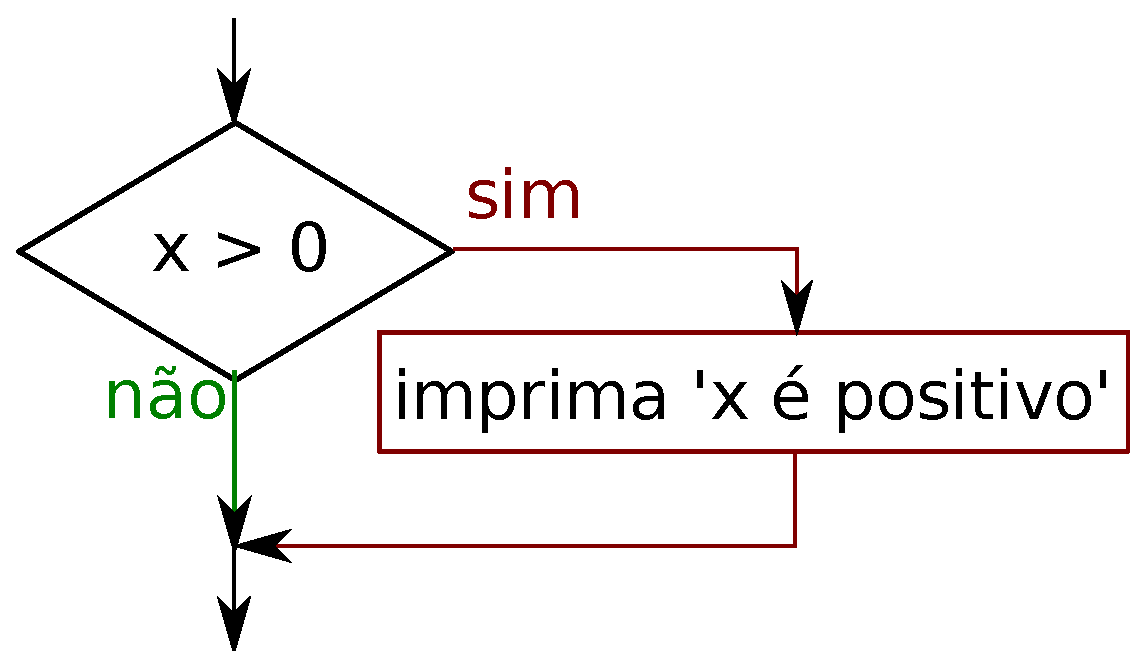
\includegraphics[height=1.75in]{figs2/if.eps}}
\afterfig

Se a condição lógica é verdadeira, então a instrução
identada é executada. Se a condição lógica é
falsa, a instrução identada é ignorada.

% If the logical condition is true, then the indented
% statement gets executed.  If the logical condition is 
% false, the indented statement is skipped.

\index{condição}
\index{declaração composta}
\index{declaração!composta}
% \index{condition}
% \index{compound statement}
% \index{statement!compound}

Instruções {\tt if} têm a mesma estrutura que as definições de funções
ou loops {\tt for} \footnote{Vamos aprender sobre as funções no Capítulo 4
e loops no Capítulo 5.}. A instrução é composta por uma linha de cabeçalho
que termina com o caractere dois pontos (:)
seguido por um bloco identado. Instruções como esta são
chamadas {\bf declarações compostas} porque elas são compostas
por mais de uma linha.

% {\tt if} statements have the same structure as function definitions
% or {\tt for} loops\footnote{We will learn about functions in Chapter 4
% and loops in Chapter 5.}.The statement consists of a header line
% that ends with the colon character (:) 
% followed by an indented block.  Statements like this are
% called {\bf compound statements} because they stretch 
% across more than one line.

Não há limite para o número de intruções que podem aparecer 
no corpo, mas deve haver pelo menos uma.
Às vezes, é util ter um corpo sem instruções (usualmente
como um corpo pacificador para o código que você não tenha escrito até o momento). Nesse
caso, você pode usar a instrução {\tt pass}, que não faz nada.

% There is no limit on the number of statements that can appear in
% the body, but there must be at least one.
% Occasionally, it is useful to have a body with no statements (usually
% as a placekeeper for code you haven't written yet).  In that
% case, you can use the {\tt pass} statement, which does nothing.

\index{instrução pass}
\index{instrução!pass}
%\index{pass statement}
%\index{statement!pass}

\beforeverb
\begin{verbatim}
if x < 0 :
    pass          # precisa lidar com valores negativos!
\end{verbatim}
%\begin{verbatim}
%if x < 0 :
%    pass          # need to handle negative values!
%\end{verbatim}
\afterverb
%
Se você digitar um {\tt if} no interpretador Python, o prompt vai se modificar
de três sinais >>> para três pontos ... para indicar que você está no meio de um bloco de
declarações, como mostrado abaixo:
% If you enter an {\tt if} statement in the Python interpreter, the prompt will change 
% from three chevrons to three dots to indicate you are in the middle of a block of
% statements, as shown below:

\beforeverb
\begin{verbatim}
>>> x = 3
>>> if x < 10:
...    print 'pequeno'
... 
Small
>>>
\end{verbatim}
%\begin{verbatim}
%>>> x = 3
%>>> if x < 10:
%...    print 'Small'
%... 
%Small
%>>>
%\end{verbatim}
\afterverb
%

\section{Execução alternativa}
\label{execucao alternativa}
%\section{Alternative execution}
%\label{alternative execution}

\index{execução alternativa}
\index{else keyword}
\index{keyword!else}
%\index{alternative execution}
%\index{else keyword}
%\index{keyword!else}

A segunda forma da instrução {\tt if} é a {\bf execução alternativa},
na qual há duas possibilidades e a condição determina
qual delas será executada. A sintaxe se parece com esta:

%A second form of the {\tt if} statement is {\bf alternative execution},
%in which there are two possibilities and the condition determines
%which one gets executed.  The syntax looks like this:

\beforeverb
\begin{verbatim}
if x%2 == 0 :
    print 'x ainda é'
else :
    print 'x é estranho'
\end{verbatim}
%\begin{verbatim}
%if x%2 == 0 :
%    print 'x is even'
%else :
%    print 'x is odd'
%\end{verbatim}
\afterverb
%

Se o resto da divisão de {\tt x} por 2 for 0, nós
sabemos que {\tt x} é divisível, e o programa exibe uma mensagem para esse
efeito. Se a condição for falsa, o segundo conjunto de instruções é
executado.

%If the remainder when {\tt x} is divided by 2 is 0, then we
%know that {\tt x} is even, and the program displays a message to that
%effect.  If the condition is false, the second set of statements is
%executed.  

\beforefig
\centerline{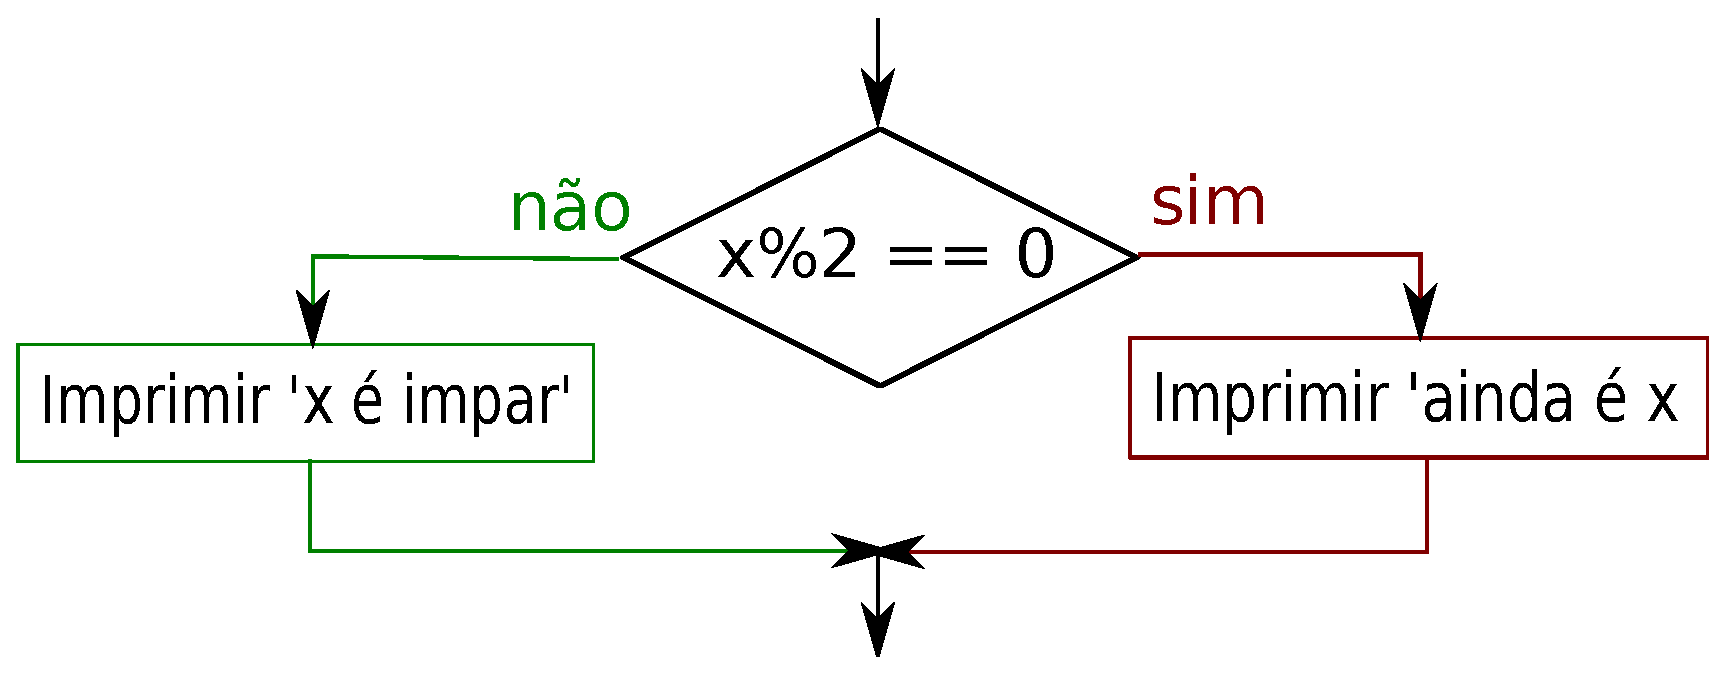
\includegraphics[height=1.75in]{figs2/if-else.eps}}
\afterfig

Uma vez que a condição deve ser verdadeira ou falsa, exatamente uma das
alternativas será executada. As alternativas são chamadas de
{\bf branches}, porque elas dividem o fluxo de execução.
%Since the condition must either be true or false, exactly one of
%the alternatives will be executed.  The alternatives are called
%{\bf branches}, because they are branches in the flow of execution.

\index{branch}

\section{Condicionais encadeadas}
%\section{Chained conditionals}
\index{chained conditional}
\index{conditional!chained}

Às vezes, há mais de duas possibilidades e precisamos de mais do que
duas condições. Uma maneira de expressar uma computação como essa é uma {\bf
condição encadeada}:
%Sometimes there are more than two possibilities and we need more than
%two branches.  One way to express a computation like that is a {\bf
%chained conditional}:

\beforeverb
\begin{verbatim}
if x < y:
    print 'x é menor que y'
elif x > y:
    print 'x é maior que y'
else:
    print 'x e y são iguais'
\end{verbatim}
\afterverb
%\begin{verbatim}
%if x < y:
%    print 'x is less than y'
%elif x > y:
%    print 'x is greater than y'
%else:
%    print 'x and y are equal'
%\end{verbatim}
\afterverb
%

{\tt elif} é uma abreviação de `` else if. '' Mais uma vez, exatamente uma
condição será executada.
%{\tt elif} is an abbreviation of ``else if.''  Again, exactly one
%branch will be executed.  

\beforefig
\centerline{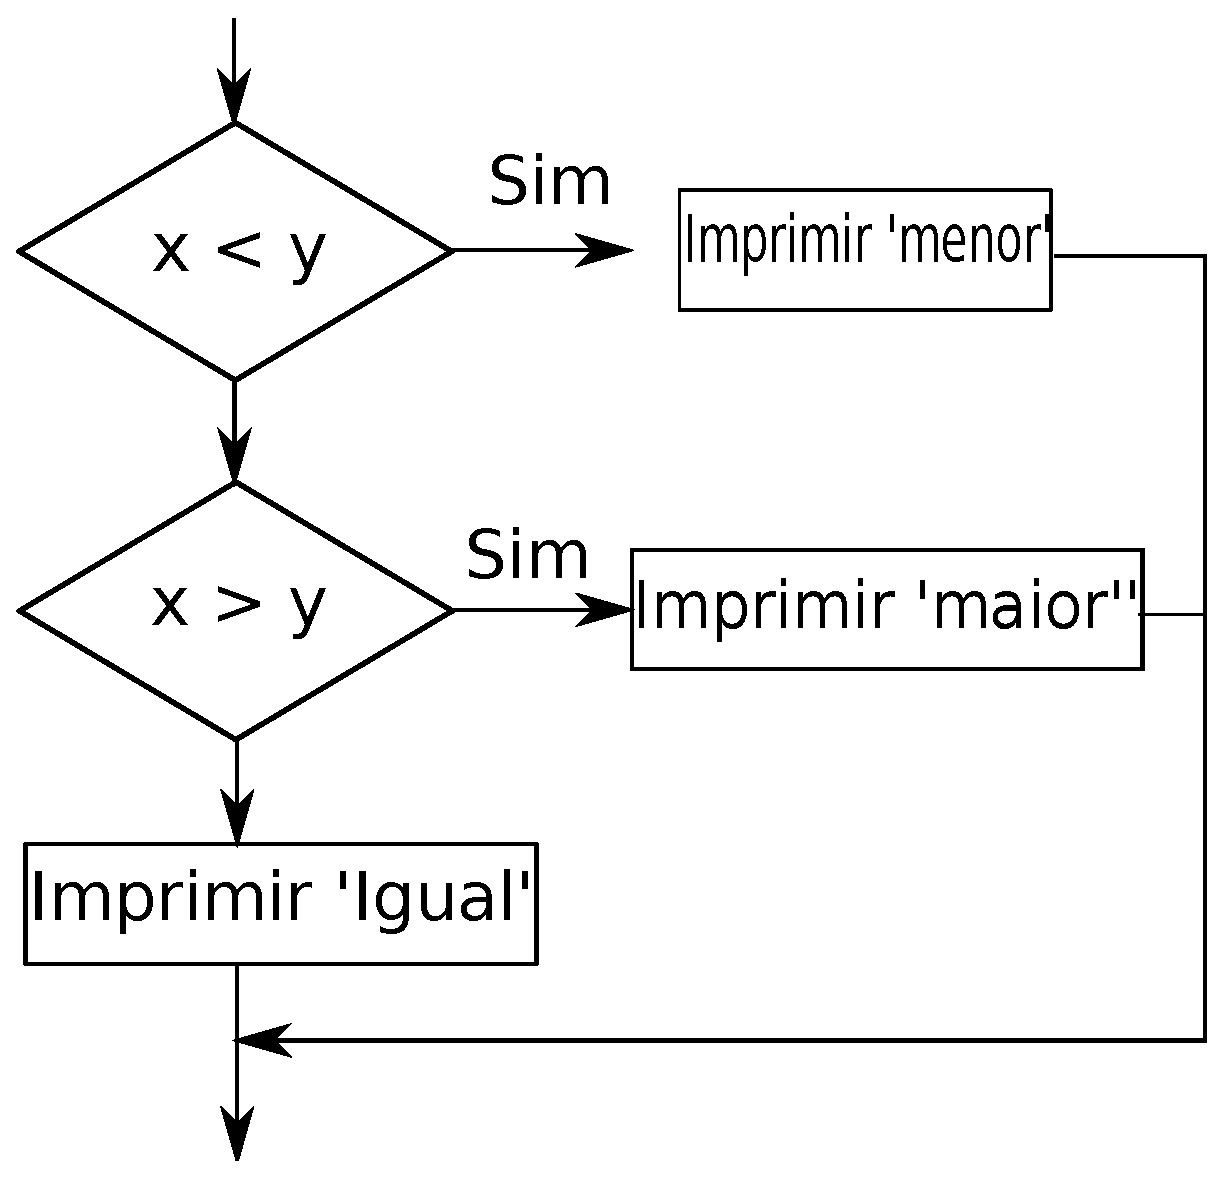
\includegraphics[height=3.00in]{figs2/elif.eps}}
\afterfig

Não há limite para o número de instruções {\tt
elif}. Se houver uma cláusula {\tt else}, ela deve estar no final,
mas só pode existir uma única instrução deste tipo.

%There is no limit on the number of {\tt
%elif} statements.  If there is an {\tt else} clause, it has to be
%at the end, but there doesn't have to be one.

\index{elif keyword}
\index{keyword!elif}
%\index{elif keyword}
%\index{keyword!elif}

\beforeverb
\begin{verbatim}
if choice == 'a':
    print 'Escolha ruim'
elif choice == 'b':
    print 'Boa escolha'
elif choice == 'c':
    print 'Perto, mas não correto'
\end{verbatim}
%\begin{verbatim}
%if choice == 'a':
%    print 'Bad guess'
%elif choice == 'b':
%    print 'Good guess'
%elif choice == 'c':
%    print 'Close, but not correct'
%\end{verbatim}
\afterverb
%

Cada condição é verificada em ordem. Se a primeira é falsa,
a próxima será avaliada, e assim por diante. Se um deles é
verdadeiro, o fluxo correspondente será executado, e a instrução
termina. Mesmo se mais do que uma condição for verdadeira, apenas o
primeiro fluxo verdadeiro é executado.

%Each condition is checked in order.  If the first is false,
%the next is checked, and so on.  If one of them is
%true, the corresponding branch executes, and the statement
%ends.  Even if more than one condition is true, only the
%first true branch executes.  


\section{Condicionais aninhados}
%\section{Nested conditionals}

\index{condicional aninhado}
\index{condicional!aninhado}
%\index{nested conditional}
%\index{conditional!nested}

Uma instrução condicional também pode ser aninhada dentro de outra. 
Nós poderíamos ter escrito o exemplo de três ramificações como a seguir:

%One conditional can also be nested within another.  We could have
%written the three-branch example like this:

\beforeverb
\begin{verbatim}
if x == y:
    print 'x e y são iguais'
else:
    if x < y:
        print 'x é menor que y'
    else:
        print 'x é maior que y'
\end{verbatim}
%\begin{verbatim}
%if x == y:
%    print 'x and y are equal'
%else:
%    if x < y:
%        print 'x is less than y'
%    else:
%        print 'x is greater than y'
%\end{verbatim}
\afterverb
%
A condicional externa contém duas ramificações. A
primeira ramificação contém uma instrução simples. A segunda ramificação
contém outra instrução {\tt if}, que contém duas ramificações
próprias. Aquelas duas ramificações são ambas instruções simples,
embora pudessem ter sido instruções condicionais também.

%The outer conditional contains two branches.  The
%first branch contains a simple statement.  The second branch
%contains another {\tt if} statement, which has two branches of its
%own.  Those two branches are both simple statements,
%although they could have been conditional statements as well.

\beforefig
\centerline{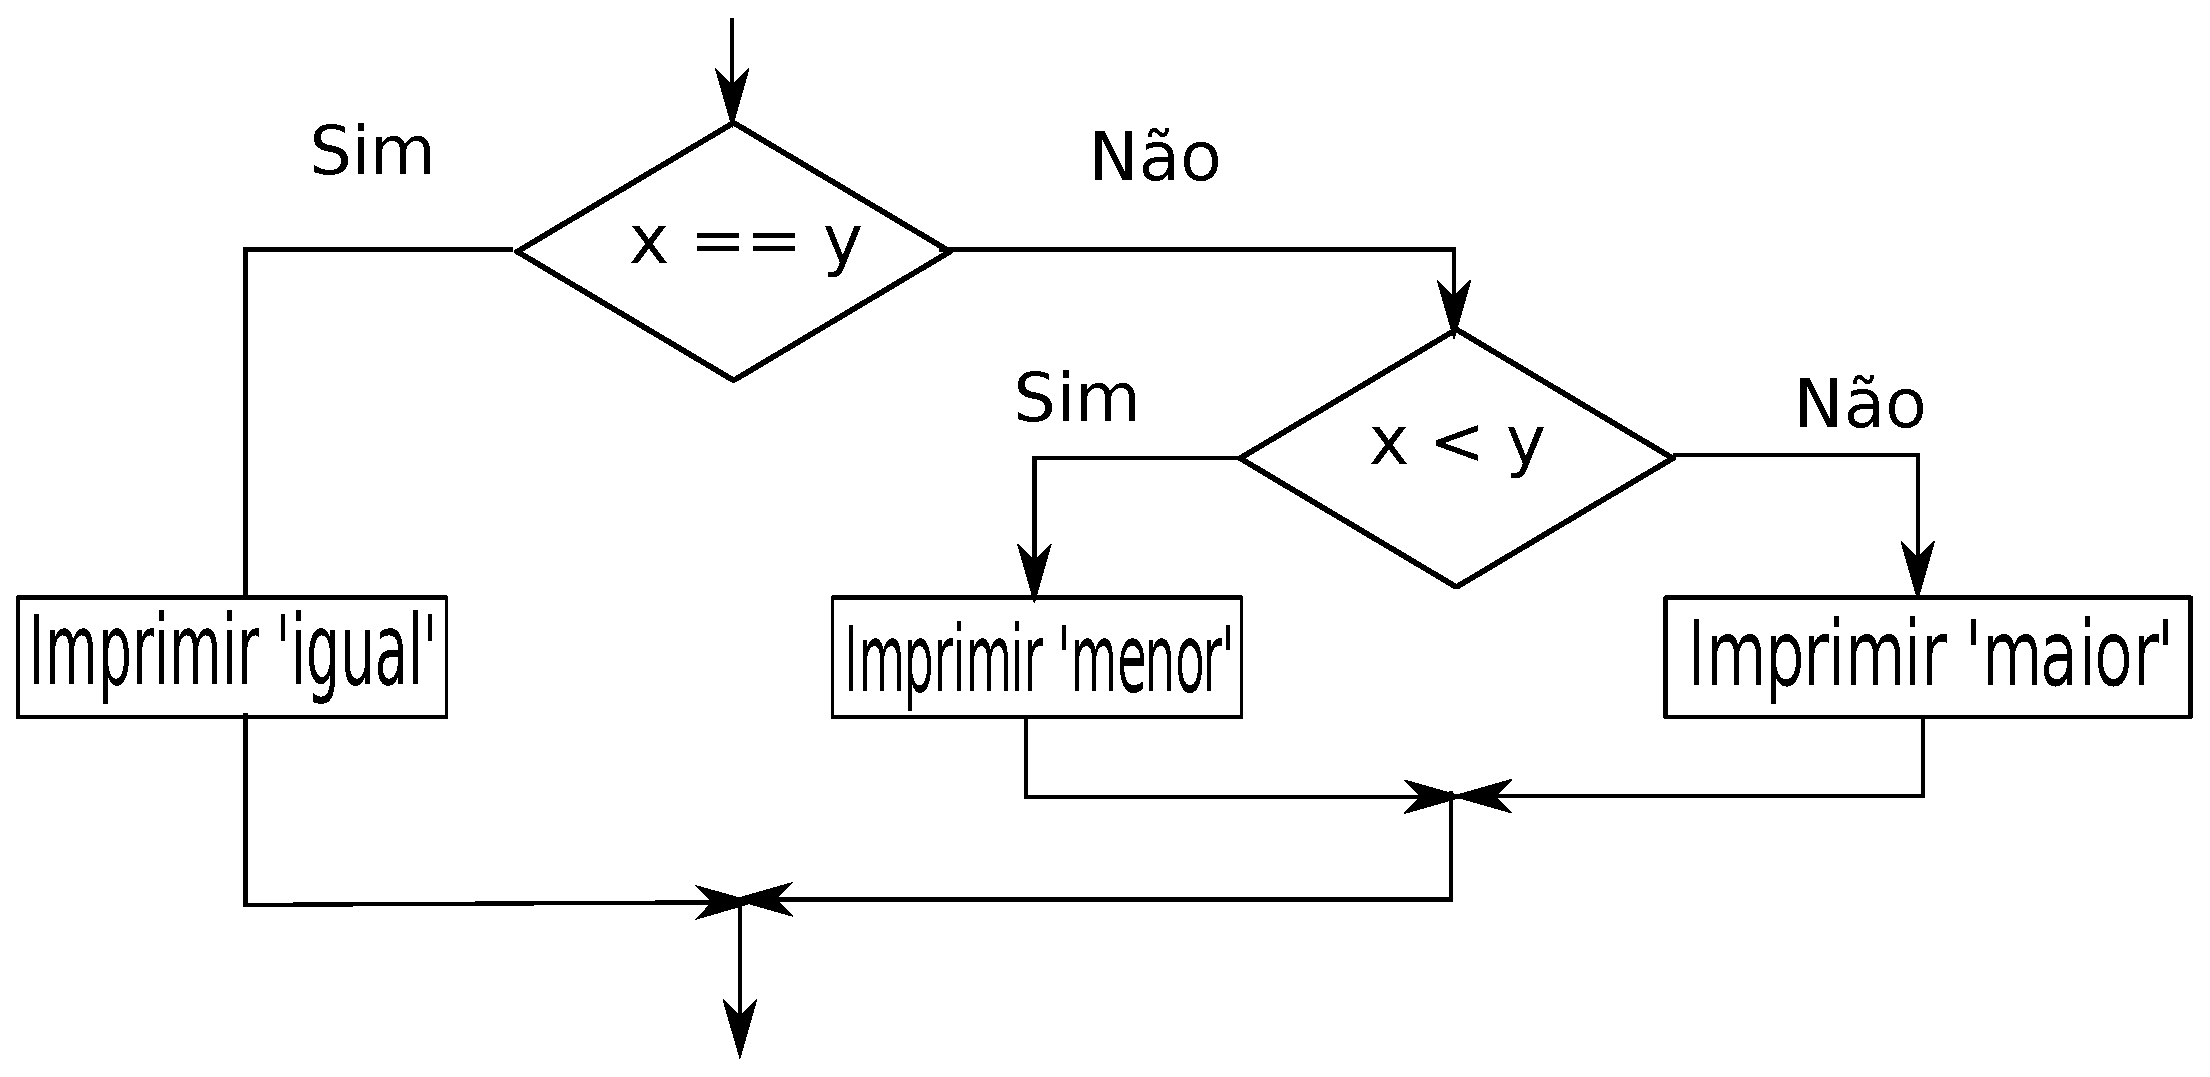
\includegraphics[height=2.50in]{figs2/nested.eps}}
\afterfig


Embora a identação das instruções torna a estrutura
visível, {\bf condicionais aninhadas} fica difícil de ler muito
rapidamente. Em geral, é uma boa idéia evitá-las sempre que possível.

%Although the indentation of the statements makes the structure
%apparent, {\bf nested conditionals} become difficult to read very
%quickly. In general, it is a good idea to avoid them when you can.


Os operadores lógicos muitas vezes fornecem uma maneira de simplificar as instruções
condicionais aninhadas. Por exemplo, podemos reescrever o código a seguir usando um
condicional simples:

%Logical operators often provide a way to simplify nested conditional
%statements.  For example, we can rewrite the following code using a
%single conditional:

\beforeverb
\begin{verbatim}
if 0 < x:
    if x < 10:
        print 'x é um número positivo de um dígito.'
\end{verbatim}
%\begin{verbatim}
%if 0 < x:
%    if x < 10:
%        print 'x is a positive single-digit number.'
%\end{verbatim}
%\afterverb
%
A instrução {\tt print} é executada somente se ambas as condições forem 
verdadeiras, para que possamos obter o mesmo efeito com o operador {\tt and}:

%The {\tt print} statement is executed only if we make it past both
%conditionals, so we can get the same effect with the {\tt and} operator:

\beforeverb
\begin{verbatim}
if 0 < x and x < 10:
    print 'x é um número positivo de um dígito.'
\end{verbatim}
%\begin{verbatim}
%if 0 < x and x < 10:
%    print 'x is a positive single-digit number.'
%\end{verbatim}
\afterverb

\section{Capturando exceções usando try e except}
%\section{Catching exceptions using try and except}
\label{catch1}

Anteriormente, vimos um segmento de código onde foram utilizadas as
funções \verb"raw_input" e {\tt int} para ler e validar um 
número inteiro informado pelo usuário. 
Também vimos como pode ser traiçoeiro utilizar isso:

%Earlier we saw a code segment where we used the \verb"raw_input" and
%{\tt int} functions to read and parse an integer number entered by
%the user.  We also saw how treacherous doing this could be:

\beforeverb
\begin{verbatim}
>>> speed = raw_input(prompt)
Qual é ... a velocidade aerodinâmica de uma andorinha sem carga?
Você quer saber, uma andorinha Africana ou Européia?
>>> int(speed)
ValueError: invalid literal for int()
>>>
\end{verbatim}
\afterverb
%\begin{verbatim}
%>>> speed = raw_input(prompt)
%What...is the airspeed velocity of an unladen swallow?
%What do you mean, an African or a European swallow?
%>>> int(speed)
%ValueError: invalid literal for int()
%>>>
%\end{verbatim}
%
Quando estamos executando estas instruções no interpretador Python,
temos um novo prompt do interpretador, acho que ``oops'', e move-se
para a próxima instrução.

%When we are executing these statements in the Python interpreter, 
%we get a new prompt from the interpreter, think ``oops'', and move 
%on to our next statement.  

No entanto, se você colocar esse código em um
script Python e este erro ocorrer, seu script para imediatamente
e nos retorna sua pilha de execução.
Não foi executada a seguinte instrução.

%However if you place this code in a 
%Python script and this error occurs, your script immediately 
%stops in its tracks with a traceback.  
%It does not execute the following statement. 
\index{traceback}


Aqui está um programa de exemplo para converter uma temperatura Fahrenheit
para uma temperatura em graus Celsius:

%Here is a sample program to convert a Fahrenheit temperature 
%to a Celsius temperature:
\index{fahrenheit}
\index{celsius}
\index{conversão de temperatura}

\beforeverb
\begin{verbatim}
inp = raw_input('Digite a Temperatura Fahrenheit:')
fahr = float(inp)
cel = (fahr - 32.0) * 5.0 / 9.0
print cel
\end{verbatim}
%\begin{verbatim}
%inp = raw_input('Enter Fahrenheit Temperature:')
%fahr = float(inp)
%cel = (fahr - 32.0) * 5.0 / 9.0
%print cel
%\end{verbatim}
\afterverb
%

Se nós executarmos este código e informarmos uma entrada inválida, ele simplesmente falha
com uma mensagem de erro não amigável:

%If we execute this code and give it invalid input, it simply fails
%with an unfriendly error message:

\beforeverb
\begin{verbatim}
python fahren.py 
Digite a Temperatura Fahrenheit:72
22.2222222222

python fahren.py 
Digite a Temperatura Fahrenheit:fred
Traceback (most recent call last):
  File "fahren.py", line 2, in <module>
    fahr = float(inp)
ValueError: invalid literal for float(): fred
\end{verbatim}
\afterverb
%\begin{verbatim}
%python fahren.py 
%Enter Fahrenheit Temperature:72
%22.2222222222

%python fahren.py 
%Enter Fahrenheit Temperature:fred
%Traceback (most recent call last):
%  File "fahren.py", line 2, in <module>
%    fahr = float(inp)
%ValueError: invalid literal for float(): fred
%\end{verbatim}
%

Existe uma estrutura de execução condicional do
Python para lidar com esses tipos esperados e inesperados de
erros chamados ``try / except''. A ideia de {\tt try}
e {\tt except} é a de que você saiba que alguma sequência
de instrução pode ter algum problema e você queira
adicionar algumas instruções para serem executadas, caso um erro ocorra.
Estas instruções adicionais (dentro do bloco except) são ignoradas
se não ocorrer um erro.

%There is a conditional execution structure built into 
%Python to handle these types of expected and unexpected
%errors called ``try / except''.  The idea of {\tt try}
%and {\tt except} is that you know that some sequence
%of instruction(s) may have a problem and you want to 
%add some statements to be executed if an error occurs.
%These extra statements (the except block) are ignored
%if there is no error.

Você pode associar os recursos {\tt try} e {\tt except}
do Python como sendo uma ``política segura'' em uma seqüência de
instruções.

%You can think of the {\tt try} and {\tt except} feature
%in Python as an ``insurance policy'' on a sequence of
%statements.

Podemos reescrever nosso conversor de temperaturas da seguinte forma:
%We can rewrite our temperature converter as follows:

\beforeverb
\begin{verbatim}
inp = raw_input('Digite a Temperatura Fahrenheit:')
try:
    fahr = float(inp)
    cel = (fahr - 32.0) * 5.0 / 9.0
    print cel
except:
    print 'Por favor, digite um numero'
\end{verbatim}
\afterverb
%

Python começa executando a
sequência de instruções dentro do
bloco {\tt try}. Se tudo correr
bem, ele ignora o bloco {\tt except} e prossegue. Se uma
exceção ocorre no bloco {\tt try},
o Python pula para fora do bloco {\tt try} e
executa a sequência de instruções do bloco {\tt except}.

%Python starts by executing the 
%sequence of statements in the 
%{\tt try} block.  If all goes
%well, it skips the {\tt except} block and proceeds.  If an
%exception occurs in the {\tt try} block, 
%Python jumps out of the {\tt try} block and
%xecutes the sequence of statements in the {\tt except} block.

\beforeverb
\begin{verbatim}
python fahren2.py 
Digite a Temperatura Fahrenheit:72
22.2222222222

python fahren2.py 
Digite a Temperatura Fahrenheit:fred
Por favor, digite um numero
\end{verbatim}
\afterverb
%

Tratar uma exceção com uma instrução {\tt try} é chamado de {\bf capturar} uma
exceção.
Neste exemplo, a cláusula {\tt except} imprime uma mensagem de erro. Em geral,
capturar uma exceção oferece a oportunidade de corrigir o problema, ou tentar
novamente, ou pelo menos terminar o programa elegantemente.

%Handling an exception with a {\tt try} statement is called {\bf
%catching} an exception.  In this example, the {\tt except} clause
%prints an error message.  In general,
%catching an exception gives you a chance to fix the problem, or try
%again, or at least end the program gracefully.

\section{Short-circuit avaliação de expressões lógicas}
%\section{Short-circuit evaluation of logical expressions}
\index{short circuit}


Quando o Python está processando uma expressão lógica, tal como
{\tt x >= 2 e (x / y) > 2}, ele avalia a expressão
da esquerda para a direita. Devido à definição do {\tt and},
se {\tt x} é inferior a 2, a expressão {\tt x >= 2} é
{\tt False} e assim toda a expressão é {\tt False} independentemente
de saber se {\tt (x / y) > 2} é avaliada como {\tt True} ou {\tt False}.

%When Python is processing a logical expression such as 
%{\tt x >= 2 and (x/y) > 2}, it evaluates the expression
%from left to right.  Because of the definition of {\tt and},
%if {\tt x} is less than 2, the expression {\tt x >= 2} is 
%{\tt False} and so the whole expression is {\tt False} regardless
%of whether {\tt (x/y) > 2} evaluates to {\tt True} or {\tt False}.

Quando o Python detecta que não existe nenhum ganho em se avaliar o 
resto de uma expressão lógica, ele para a sua avaliação e não 
faz os cálculos para o restante da expressão lógica.
Quando a avaliação de uma expressão lógica para porque o valor global já 
é conhecido, a avaliação é chamada de {\bf short-circuiting}.

%When Python detects that there is nothing to be gained by evaluating
%the rest of a logical expression, it stops its evaluation and does
%not do the computations in the rest of the logical expression.  
%When the evaluation of a logical expression stops because the overall
%value is already known, it is called {\bf short-circuiting} 
%the evaluation.

\index{guardian pattern}
\index{pattern!guardian}

Embora esta técnica pareça ter pouca importância, o comportamento de short-circuit
leva a uma técnica inteligente chamada {\bf guardian pattern}.
Considere a seguinte sequência de código no interpretador Python:
%While this may seem like a fine point, the short-circuit behavior
%leads to a clever technique called the {\bf guardian pattern}.  
%Consider the following code sequence in the Python interpreter:

\beforeverb
\begin{verbatim}
>>> x = 6 
>>> y = 2
>>> x >= 2 and (x/y) > 2
True
>>> x = 1 
>>> y = 0
>>> x >= 2 and (x/y) > 2
False
>>> x = 6
>>> y = 0
>>> x >= 2 and (x/y) > 2
Traceback (most recent call last):
  File "<stdin>", line 1, in <module>
ZeroDivisionError: integer division or modulo by zero
>>> 
\end{verbatim}
%\begin{verbatim}
%>>> x = 6 
%>>> y = 2
%>>> x >= 2 and (x/y) > 2
%True
%>>> x = 1 
%>>> y = 0
%>>> x >= 2 and (x/y) > 2
%False
%>>> x = 6
%>>> y = 0
%>>> x >= 2 and (x/y) > 2
%Traceback (most recent call last):
%  File "<stdin>", line 1, in <module>
%ZeroDivisionError: integer division or modulo by zero
%>>> 
%\end{verbatim}
\afterverb
%
O terceiro cálculo falhou porque o Python estava avaliando {\tt (x/y)}
e {\tt y} foi zero, o que causou um erro de execução. Mas o segundo exemplo
\emph{não} falhou porque a primeira parte da expressão {\tt x >= 2} foi
avaliada como {\tt False} então a expressão {\tt (x/y)} não foi executada
devido à regra {\bf short-circuit} e não houve erro.

%The third calculation failed because Python was evaluating {\tt (x/y)}
%and {\tt y} was zero, which causes a runtime error.  But the second example
%did \emph{not} fail because the first part of the expression {\tt x >= 2} 
%evaluated to {\tt False} so the {\tt (x/y)} was not ever executed 
%due to the {\bf short-circuit} rule and there was no error.


Podemos construir a expressão lógica para colocar estrategicamente uma avaliação 
do tipo {\bf guardian pattern} antes da avaliação que pode causar um erro, como segue:

%We can construct the logical expression to strategically place a {\bf guard}
%evaluation just before the evaluation that might cause an error as follows:

\beforeverb
\begin{verbatim}
>>> x = 1
>>> y = 0
>>> x >= 2 and y != 0 and (x/y) > 2
False
>>> x = 6 
>>> y = 0
>>> x >= 2 and y != 0 and (x/y) > 2
False
>>> x >= 2 and (x/y) > 2 and y != 0
Traceback (most recent call last):
  File "<stdin>", line 1, in <module>
ZeroDivisionError: integer division or modulo by zero
>>>
\end{verbatim}
%\begin{verbatim}
%>>> x = 1
%>>> y = 0
%>>> x >= 2 and y != 0 and (x/y) > 2
%False
%>>> x = 6 
%>>> y = 0
%>>> x >= 2 and y != 0 and (x/y) > 2
%False
%>>> x >= 2 and (x/y) > 2 and y != 0
%Traceback (most recent call last):
%  File "<stdin>", line 1, in <module>
%ZeroDivisionError: integer division or modulo by zero
%>>>
%\end{verbatim}
\afterverb
%

Na primeira expressão lógica, {\tt x >= 2} é {\tt False}, então a avaliação
para no {\tt and}. Na segunda expressão lógica, {\tt x >= 2} é {\tt True}
mas {\tt y != 0} é {\tt False} então nunca chegamos a avaliar a expressão {\tt (x/y)}.

%In the first logical expression, {\tt x >= 2} is {\tt False} so the evaluation
%stops at the {\tt and}.  In the second logical expression, {\tt x >= 2} is {\tt True}
%but {\tt y != 0} is {\tt False} so we never reach {\tt (x/y)}.


Na terceira expressão lógica, o {\tt y != 0} encontra-se \emph{depois} do cálculo
{\tt (x/y) } de modo que a expressão termina com um erro.

%In the third logical expression, the {\tt y != 0} is \emph{after} the 
%{\tt (x/y) } calculation so the expression fails with an error.


Na segunda expressão, dizemos que {\tt y != 0} atua como um {\bf guard}
para garantir que só executaremos {{\tt (x/y)} se {\tt y} for diferente de zero.

%In the second expression, we say that {\tt y != 0} acts as a {\bf guard}
%to insure that we only execute {\tt (x/y)} if {\tt y} is non-zero.

\section{Depuração}
%\section{Debugging}

\label{whitespace}

\index{debugging}
\index{traceback}

O Python traceback é exibido quando ocorre um erro, ele contém
diversas informações, mas pode ser um pouco confuso com tantos
dados. A maioria das informações úteis geralmente são:

%The traceback Python displays when an error occurs contains
%a lot of information, but it can be overwhelming.  The most
%useful parts are usually:

\begin{itemize}

\item Que tipo de erro ocorreu, e

\item Onde ocorreu.

\end{itemize}
%\begin{itemize}

%\item What kind of error it was, and

%\item Where it occurred.

%\end{itemize}

Erros de sintaxe geralmente são fáceis de encontrar, mas há algumas
pegadinhas. Erros por espaço em branco podem ser difíceis, porque os espaços e
tabs são invisíveis e geralmente os ignoramos.

%Syntax errors are usually easy to find, but there are a few
%gotchas.  Whitespace errors can be tricky because spaces and
%tabs are invisible and we are used to ignoring them.

\index{whitespace}

\beforeverb
\begin{verbatim}
>>> x = 5
>>>  y = 6
  File "<stdin>", line 1
    y = 6
    ^
SyntaxError: invalid syntax
\end{verbatim}
%\begin{verbatim}
%>>> x = 5
%>>>  y = 6
%  File "<stdin>", line 1
%    y = 6
%    ^
%SyntaxError: invalid syntax
%\end{verbatim}
\afterverb
%
Neste exemplo, o problema é que a segunda linha é indentada por
um espaço. Mas a mensagem de erro aponta para {\tt y}, que é
enganosa. Em geral, as mensagens de erro indicam onde o problema foi
descoberto, mas o erro real pode estar no início do código,
às vezes em uma linha anterior.

%In this example, the problem is that the second line is indented by
%one space.  But the error message points to {\tt y}, which is
%misleading.  In general, error messages indicate where the problem was
%discovered, but the actual error might be earlier in the code,
%sometimes on a previous line.

\index{erro!execução}
\index{erro de execução}

O mesmo ocorre para erros de execução. Suponha que você está tentando
calcular uma relação sinal-ruído em decibéis. A fórmula
é $SNR_{db} = 10 \log_{10} (P_{signal} / P_{noise})$. Em Python,
você pode escrever algo como isto:

%The same is true of runtime errors.  Suppose you are trying
%to compute a signal-to-noise ratio in decibels.  The formula
%is $SNR_{db} = 10 \log_{10} (P_{signal} / P_{noise})$.  In Python,
%you might write something like this:

\beforeverb
\begin{verbatim}
import math
signal_power = 9
noise_power = 10
ratio = signal_power / noise_power
decibels = 10 * math.log10(ratio)
print decibels
\end{verbatim}
\afterverb
%
Mas quando você executá-lo, você recebe uma mensagem de erro \footnote{Em Python 3.0,
   você não recebe uma mensagem de erro; o operador de divisão executa a
   divisão de ponto flutuante, mesmo com operandos do tipo inteiro.}:

%But when you run it, you get an error message\footnote{In Python 3.0,
%  you no longer get an error message; the division operator performs
%  floating-point division even with integer operands.}:

\index{exceção!OverflowError}
\index{OverflowError}

\beforeverb
\begin{verbatim}
Traceback (most recent call last):
  File "snr.py", line 5, in ?
    decibels = 10 * math.log10(ratio)
OverflowError: math range error
\end{verbatim}
%\begin{verbatim}
%Traceback (most recent call last):
%  File "snr.py", line 5, in ?
%    decibels = 10 * math.log10(ratio)
%OverflowError: math range error
%\end{verbatim}
\afterverb
%

A mensagem de erro indica a linha 5, mas não há nada
errado com essa linha. Para encontrar o verdadeiro erro, pode ser
útil imprimir o valor da variável {\tt ratio}, que daria 
0. O problema está na linha 4, porque dividir dois inteiros
causa ``floor division''''. A solução é representar a potência do sinal
e potência de ruído com valores de ponto flutuante.

%The error message indicates line 5, but there is nothing
%wrong with that line.  To find the real error, it might be
%useful to print the value of {\tt ratio}, which turns out to
%be 0.  The problem is in line 4, because dividing two integers
%does floor division.  The solution is to represent signal power
%and noise power with floating-point values.

\index{floor division}
\index{division!floor}

Em geral, mensagens de erro dizem onde o problema foi descoberto,
mas frequentemente não dizem onde ele foi causado.

%In general, error messages tell you where the problem was discovered, 
%but that is often not where it was caused.


\section{Glossário}
%\section{Glossary}

\begin{description}

\item[body:] Uma sequência de instruções dentro de uma instrução composta
%\item[body:] The sequence of statements within a compound statement.
\index{body}

\item[boolean expression:] Uma expressão cujo valor é
{\tt True} ou {\tt False}.
%\item[boolean expression:]  An expression whose value is either 
%{\tt True} or {\tt False}.
\index{boolean expression}
\index{expression!boolean}

\item[branch:] Uma das sequências alternativas de instruções em uma 
instrução condicional.
%\item[branch:] One of the alternative sequences of statements in
%a conditional statement.
\index{branch}

\item[condicional encadeada:]  Uma instrução condicional com uma série 
de ramificações alternativas.
%\item[chained conditional:]  A conditional statement with a series
%of alternative branches.
\index{condicional encadeada}
\index{condicional!encadeada}

\item[operador de comparação:] Um dos operadores que compara 
seus operandos: {\tt ==}, {\tt !=}, {\tt >}, {\tt <}, {\tt >=}, and {\tt <=}.
%\item[comparison operator:] One of the operators that compares
%its operands: {\tt ==}, {\tt !=}, {\tt >}, {\tt <}, {\tt >=}, and {\tt <=}.

\item[instrução condicional:] Uma declaração que controla o fluxo de 
execução dependendo de alguma condição
%\item[conditional statement:]  A statement that controls the flow of
%execution depending on some condition.
\index{instrução condicional}
\index{instrução!condicional}

\item[condição:] A expressão booleana em uma declaração condicional 
que determina qual a condição é executado.
%\item[condition:] The boolean expression in a conditional statement
%that determines which branch is executed.
\index{condição}

\item[instrução composta:] Uma declaração que consiste de um cabeçalho 
e um corpo. O cabeçalho termina com dois pontos (:). O corpo é identado em 
relação ao cabeçalho.
%\item[compound statement:]  A statement that consists of a header
%and a body.  The header ends with a colon (:).  The body is indented
%relative to the header.
\index{instrução composta}

\item[guardian pattern:] Onde nós construimos uma expressão lógica com 
comparações adicionais para aproveitar o comportamento de short-circuit.
%\item[guardian pattern:] Where we construct a logical expression 
%with additional
%comparisons to take advantage of the short-circuit behavior.
\index{guardian pattern}
\index{pattern!guardian}

\item[operador lógico:] Um dos operadores que combina expressões 
booleanas: {\tt and}, {\tt or}, e {\tt not}.
%\item[logical operator:] One of the operators that combines boolean
%expressions: {\tt and}, {\tt or}, and {\tt not}.

\item[condicional aninhada:] Uma instrução condicional que aparece em um dos 
ramos de uma outra instrução condicional.
%\item[nested conditional:]  A conditional statement that appears
%in one of the branches of another conditional statement.
\index{condicional aninhada}
\index{condicional!aninhada}

\item[traceback:] Uma lista das funções que estão em execução, 
impressa quando ocorre uma exceção.
%\item[traceback:]  A list of the functions that are executing,
%printed when an exception occurs.
\index{traceback}

\item[short circuit:] Quando o Python deixa de avaliar uma expressão 
lógica atéo final e para porque já sabe o valor final para a expressão
sem a necessidade de avaliar o resto da expressão.
%\item[short circuit:]  When Python is part-way through evaluating a 
%logical expression and stops the evaluation because Python 
%knows the final value for the expression 
%without needing to evaluate the rest of the expression.
\index{short circuit}

\end{description}

\section{Exercícios}
%\section{Exercises}

\begin{ex}
Reescrever o seu cálculo de pagamento para dar ao trabalhador 1.5
vezes o valor da hora para
horas trabalhadas acima de 40 horas.
%Rewrite your pay computation to give the employee 1.5 
%times the hourly rate for 
%hours worked above 40 hours.

\begin{verbatim}
Digite as Horas: 45
Digite a Taxa: 10
Pagamento: 475.0
\end{verbatim}
\end{ex}
%\begin{verbatim}
%Enter Hours: 45
%Enter Rate: 10
%Pay: 475.0
%\end{verbatim}
%\end{ex}

\begin{ex}
Reescrever seu programa de pagamento usando {\tt try} e {\tt except} 
para que o programa trate entradas não numérica amigavelmente
imprimindo uma mensagem e saindo do programa.
A seguir mostra duas execuções do programa:
%Rewrite your pay program using {\tt try} and {\tt except} 
%so that your program handles non-numeric input gracefully
%by printing a message and exiting the program.
%The following shows two executions of the program:

\begin{verbatim}
Digite as Horas: 20
Digite a Taxa: nove
Erro, por favor, informe entrada numérica

Digite as Horas: quarenta
Erro, por favor, informe entrada numérica
\end{verbatim}
\end{ex}
%\begin{verbatim}
%Enter Hours: 20
%Enter Rate: nine
%Error, please enter numeric input

%Enter Hours: forty
%Error, please enter numeric input
%\end{verbatim}
%\end{ex}

\begin{ex}
Escreva um programa para solicitar uma pontuação entre 0.0 e 1.0.
Se o resultado estiver fora da faixa, imprimir uma mensagem de erro. Se a pontuação
estiver entre 0.0 e 1.0, imprimir uma nota utilizando a seguinte tabela:
%Write a program to prompt for a score between 0.0 and 1.0.
%If the score is out of range, print an error message.  If the score
%is between 0.0 and 1.0, print a grade using the following 
%table:

\begin{verbatim}
Ponto   Nota
>= 0.9   A
>= 0.8   B
>= 0.7   C
>= 0.6   D
< 0.6    F

Digite a Pontuação: 0.95
A

Digite a Pontuação: perfeito
Pontuação incorreta

Digite a Pontuação: 10.0
Pontuação incorreta

Digite a Pontuação: 0.75
C

Digite a Pontuação: 0.5
F
\end{verbatim}
%\begin{verbatim}
%Score   Grade
%>= 0.9     A
%>= 0.8     B
%>= 0.7     C
%>= 0.6     D
%< 0.6    F

%Enter score: 0.95
%A

%Enter score: perfect
%Bad score

%Enter score: 10.0
%Bad score

%Enter score: 0.75
%C

%Enter score: 0.5
%F
%\end{verbatim}

Executar o programa repetidamente, como mostrado acima, para testar os 
diversos resultados para as diferentes entradas.
%Run the program repeatedly as shown above to test the 
%various different values for input.
\end{ex}
% TODO % LaTeX source for ``Python for Informatics: Exploring Information''
% Copyright (c)  2010-  Charles R. Severance, All Rights Reserved

%\chapter{Functions}
\chapter{Funções}
\label{funcchap}

%\section{Function calls}
\section{Chamadas de funções}
\label{functionchap}
\index{function call}

%In the context of programming, a {\bf function} is a named sequence of
%statements that performs a computation.  When you define a function,
%you specify the name and the sequence of statements.  Later, you can
%``call'' the function by name.  
%We have already seen one example of a {\bf function call}:

Em programação, uma {\bf função} é uma sequência de condições que executa uma
tarefa. Quando você define uma função, você especifica o nome e a sequência de
condições. Posteriormente, você pode ``chamar'' a função pelo nome. Nós já
vimos um exemplo de {\bf chamada de função}:

\beforeverb
\begin{verbatim}
>>> type(32)
<type 'int'>
\end{verbatim}
\afterverb
%
%The name of the function is {\tt type}.  The expression in parentheses
%is called the {\bf argument} of the function.  The argument is 
%a value or variable that we are passing into the function as input 
%to the function.  
%The result, for the {\tt type} function, is the type of the argument.
%
O nome da função é {\tt type}. A expressão em parênteses é chamada de
{\bf argumento} da função. O argumento é um valor ou variável que passamos
como entrada para a função. O resultado, para a função {\tt type}, é o tipo
do argumento.

\index{parentheses!argument in}

%It is common to say that a function ``takes'' an argument and ``returns''
%a result.  The result is called the {\bf return value}.

É comum dizer que uma função ``recebe'' um arqumento e ``retorna'' um resultado.
O resultado é chamado de {\bf valor de retorno}.


\index{argument}
\index{return value}

%\section{Built-in functions}
\section{Funções embutidas (``baterias inclusas'')}
%Python provides a number of important built-in functions that
%we can use without needing to provide the function definition.
%The creators of Python wrote a set of functions 
%to solve common problems and included them in Python for us to use.

O Python provê um grande número de funções embutidas importantes que podemos
utilizar sem a necessidade de definir como novas funções. Os criadores de
Python escreveram um conjunto de funções para a resoluções de problemas comuns
e incluiram-nas no Python para que as utilizássemos.

%The {\tt max} and {\tt min} functions give us the largest and 
%smallest values in a list, respectively:

As funções {\tt max} e {\tt min} nos dão o maior e o menor valor em uma lista,
respectivamente:

\beforeverb
\begin{verbatim}
>>> max('Hello world')
'w'
>>> min('Hello world')
' '
>>>
\end{verbatim}
\afterverb
%
%The {\tt max} function tells us the ``largest character'' in the 
%string (which turns out to be the letter ``w'') and the {\tt min}
%function shows us the smallest character (which turns out to be a 
%space).
%
A função {\tt max} retorna o ``maior caractere'' quando usado com {\it strings}
(que acaba sendo a letra ``w'') e função {\tt min} retorna o menor caractere
(que é o espaço).

%Another very common built-in function is the {\tt len} function
%which tells us how many items are in its argument. If the argument
%to {\tt len} is a string, it returns the number of characters 
%in the string.

Outra função muito comum é a função {\tt len} que nos diz quantos ítens tem
no seu argumento. Se o argumento do {\tt len} é uma {\it string}, ela vai
retornar o número de caracteres na {\it string}.

\beforeverb
\begin{verbatim}
>>> len('Hello world')
11
>>>
\end{verbatim}
\afterverb
%
%These functions are not limited to looking at strings. They can operate
%on any set of values, as we will see in later chapters.
%
Estas funções não estão limitadas ao uso com {\it strings}. Elas podem ser
utilizadas em qualquer conjunto de valores, como veremos nos próximos capítulos.

%You should treat the names of built-in functions as reserved words (i.e.,
%avoid using ``max'' as a variable name).

Você deve tratar os nomes das funções embutidas como palavras reservadas (i.e.,
evitando utilizar ``max'' como nome de variável).

%\section{Type conversion functions}
\section{Funções de conversões de tipos}
\index{conversion!type}
\index{type conversion}

% from Elkner:
% comment on whether these things are _really_ functions?
% use max as an example of a built-in?

% my reply:
% they are on the list of ``built-in functions'' so I am
% willing to call them functions.

%Python also provides built-in functions that convert values
%from one type to another.  The {\tt int} function takes any value and
%converts it to an integer, if it can, or complains otherwise:

Python também provê funções para converter valores de um tipo para outro. A
função {\tt int} pega um valor e converte para um inteiro, se ela conseguir,
caso contrário ela vai ``reclamar'':

\index{int function}
\index{function!int}

\beforeverb
\begin{verbatim}
>>> int('32')
32
>>> int('Hello')
ValueError: invalid literal for int(): Hello
\end{verbatim}
\afterverb
%
%{\tt int} can convert floating-point values to integers, but it
%doesn't round off; it chops off the fraction part:
%
A função {\tt int} pode converter um ponto-flutuante para um inteiro, mas ela
não arredonda; ela somente corta a parte fracionária:

\beforeverb
\begin{verbatim}
>>> int(3.99999)
3
>>> int(-2.3)
-2
\end{verbatim}
\afterverb
%
%{\tt float} converts integers and strings to floating-point
%numbers:
%
A função {\tt float} converte inteiros e {\it strings} para pontos-flutuantes:

\index{float function}
\index{function!float}

\beforeverb
\begin{verbatim}
>>> float(32)
32.0
>>> float('3.14159')
3.14159
\end{verbatim}
\afterverb
%
%Finally, {\tt str} converts its argument to a string:
%
E por fim, {\tt str} converte seu arqumento para uma {\it string}:

\index{str function}
\index{function!str}

\beforeverb
\begin{verbatim}
>>> str(32)
'32'
>>> str(3.14159)
'3.14159'
\end{verbatim}
\afterverb
%

%\section{Random numbers}
\section{Números aleatórios}

\index{random number}
\index{number, random}
\index{deterministic}
\index{pseudorandom}

%Given the same inputs, most computer programs generate the same
%outputs every time, so they are said to be {\bf deterministic}.
%Determinism is usually a good thing, since we expect the same
%calculation to yield the same result.  For some applications, though,
%we want the computer to be unpredictable.  Games are an obvious
%example, but there are more.

Dada a mesma entrada, a maioria dos programas de computadores geram sempre a
mesma saída, por isso são chamados de {\bf determinísticos}. Determinismo é
normalmente uma coisa boa, uma vez que esperamos que o mesmo cálculo retorne
o mesmo resultado. Para algumas aplicações, no entanto, nós desejamos que o
computador seja imprevisível. Os jogos são exemplos óbvios, mas existem outros.

%Making a program truly nondeterministic turns out to be not so easy,
%but there are ways to make it at least seem nondeterministic.  One of
%them is to use {\bf algorithms} that generate {\bf pseudorandom} numbers.
%Pseudorandom numbers are not truly random because they are generated
%by a deterministic computation, but just by looking at the numbers it
%is all but impossible to distinguish them from random.

Fazer um programa realmente não-determinístico não é uma coisa tão fácil, mas
existem formas de fazê-lo ao menos parecer não-determinístico. Umas das formas
é utilizar {\bf algoritmos} que geram números pseudoaleatórios. Números
pseudoaleatórios não são realmente aleatórios porque são gerados por uma
computação determinística, mas somente olhando para os números é quase
impossível distingui-los de números aleatórios.

\index{random module}
\index{module!random}

%The {\tt random} module provides functions that generate
%pseudorandom numbers (which I will simply call ``random'' from
%here on).

O módulo {\tt random} provê funções que geram números pseudoaleatórios (que
eu vou chamar simplesmente de ``aleatórios'' a partir de agora).

\index{random function}
\index{function!random}

%The function {\tt random} returns a random float
%between 0.0 and 1.0 (including 0.0 but not 1.0).  Each time you
%call {\tt random}, you get the next number in a long series.  To see a
%sample, run this loop:

A função {\tt random} retorna um {\it float} aleatório entre 0.0 e 1.0
(incluindo o 0.0, mas não o 1.0). Cada vez que a função {\tt random} é chamada
você obtém um número com uma grande série. Para ver um exemplo disto, execute
este laço:

\beforeverb
\begin{verbatim}
import random

for i in range(10):
    x = random.random()
    print x
\end{verbatim}
\afterverb
%
%This program produces the following list of 10 random numbers
%between 0.0 and up to but not including 1.0.
%
Este programa produziu a seguinte lista de 10 números aleatórios entre 0.0
e até, mas não incluindo, o 1.0.

\beforeverb
\begin{verbatim}
0.301927091705
0.513787075867
0.319470430881
0.285145917252
0.839069045123
0.322027080731
0.550722110248
0.366591677812
0.396981483964
0.838116437404
\end{verbatim}
\afterverb
%
\begin{ex}
%Run the program on your system and see what numbers you get.
%Run the program more than once and see what numbers you get.
Execute o programa em seu computador e veja quais números você obtém.
Execute o programa mais de uma vez no seu computador e veja quais números você obtém.
\end{ex}

%The {\tt random} function is only one of many 
%functions that handle random numbers.
%The function {\tt randint} takes the parameters {\tt low} and
%{\tt high}, and returns an integer between {\tt low} and
%{\tt high} (including both).

A função {\tt random} é uma de muitas funções que tratam números aleatórios.
A função {\tt randint} usa como parâmetros {\tt baixo} e {\tt alto}, e retorna
um inteiro entre estes números (incluindo ambos os números passados).

\index{randint function}
\index{function!randint}

\beforeverb
\begin{verbatim}
>>> random.randint(5, 10)
5
>>> random.randint(5, 10)
9
\end{verbatim}
\afterverb
%
%To choose an element from a sequence at random, you can use
%{\tt choice}:

Para escolher um elemento de uma sequência aleatória, você pode utilizar a
função {\tt choice}:

\index{choice function}
\index{function!choice}

\beforeverb
\begin{verbatim}
>>> t = [1, 2, 3]
>>> random.choice(t)
2
>>> random.choice(t)
3
\end{verbatim}
\afterverb
%
%The {\tt random} module also provides functions to generate
%random values from continuous distributions including
%Gaussian, exponential, gamma, and a few more.
%
O módulo {\tt random} também provê funções para geração de valores,
distribuições contínuas incluindo Gaussianas, exponenciais, gama e algumas
outras.

%\section{Math functions}
\section{Funções matemáticas}

\index{math function}
\index{function, math}
\index{module}
\index{module object}

%Python has a {\tt math} module that provides most of the familiar
%mathematical functions.  
%Before we can use the module, we have to import it:

Python tem o módulo {\tt math} que provê as funções matemáticas mais
conhecidas. Antes de utilizar o módulo, temos que importá-lo:

\beforeverb
\begin{verbatim}
>>> import math
\end{verbatim}
\afterverb
%
%This statement creates a {\bf module object} named math.  If
%you print the module object, you get some information about it:
%
Esta declaração cria um módulo objeto chamado math. Se você exibir o objeto
módulo, obterá algumas informações sobre ele:

\beforeverb
\begin{verbatim}
>>> print math
<module 'math' from '/usr/lib/python2.5/lib-dynload/math.so'>
\end{verbatim}
\afterverb
%
%The module object contains the functions and variables defined in the
%module.  To access one of the functions, you have to specify the name
%of the module and the name of the function, separated by a dot (also
%known as a period).  This format is called {\bf dot notation}.
%
O módulo contém funções e variáveis definidas. Para acessar umas destas
funções, tem que especificar o nome do módulo e o nome da função, separados
por um ponto (também conhecido como período). Este formato é conhecido como
{\bf notação de ponto}.

\index{dot notation}

\beforeverb
\begin{verbatim}
>>> ratio = signal_power / noise_power
>>> decibels = 10 * math.log10(ratio)

>>> radians = 0.7
>>> height = math.sin(radians)
\end{verbatim}
\afterverb
%
%The first example computes the logarithm base 10 of the
%signal-to-noise ratio.  The math module also provides a
%function called {\tt log} that computes logarithms base {\tt e}.
%
O primeiro exemplo calcula o logaritmo de base 10 da relação sinal-ruído. O
módulo {\tt math} também provê uma função chamada {\tt log} que calcula o
logaritmo de base {\tt e}.

\index{log function}
\index{function!log}
\index{sine function}
\index{radian}
\index{trigonometric function}
\index{function, trigonometric}

%The second example finds the sine of {\tt radians}.  The name of the
%variable is a hint that {\tt sin} and the other trigonometric
%functions ({\tt cos}, {\tt tan}, etc.)  take arguments in radians. To
%convert from degrees to radians, divide by 360 and multiply by $2
%\pi$:

O segundo exemplo descobre o seno de {\tt radianos}. O nome da variável é uma
dica para informar que o {\tt sin} e as outras funções trigonométricas
({\tt cos}, {\tt tan}, etc.) recebem como argumento valores em radianos. Para
converter de graus para radianos, divide-se o valor por 360 e multiplica-se
por $2 \pi$:


\beforeverb
\begin{verbatim}
>>> degrees = 45
>>> radians = degrees / 360.0 * 2 * math.pi
>>> math.sin(radians)
0.707106781187
\end{verbatim}
\afterverb
%
%The expression {\tt math.pi} gets the variable {\tt pi} from the math
%module.  The value of this variable is an approximation
%of $\pi$, accurate to about 15 digits.
%
A expressão {\tt math.pi} pega a variável {\tt pi} do módulo {\tt math}. O
valor desta variável é uma aproximação do $\pi$, em exatos 15 dígitos.

\index{pi}

%If you know
%your trigonometry, you can check the previous result by comparing it to
%the square root of two divided by two:

Se você conhece trigometria, você pode verificar o resultado anterior
comparando-o a raiz de 2 dividido por 2:

\index{sqrt function}
\index{function!sqrt}

\beforeverb
\begin{verbatim}
>>> math.sqrt(2) / 2.0
0.707106781187
\end{verbatim}
\afterverb
%


%\section{Adding new functions}
\section{Adicionando novas funções}

%So far, we have only been using the functions that come with Python,
%but it is also possible to add new functions.
%A {\bf function definition} specifies the name of a new function and
%the sequence of statements that execute when the function is called.
%Once we define a function, we can reuse the function over and over 
%throughout our program.

Até agora, utilizamos somente funções que já estão no Python, mas também é
possível adicionar novas funções. Uma definição de uma função especifica o
nome de uma nova função e a sequência das condições que serão executadas
quando a função é chamada. Uma vez definida a função, podemos reutilizá-la
diversas vezes em nosso programa.

\index{function}
\index{function definition}
\index{definition!function}

%Here is an example:

Aqui temos um exemplo:

\beforeverb
\begin{verbatim}
def print_lyrics():
    print "I'm a lumberjack, and I'm okay."
    print 'I sleep all night and I work all day.'
\end{verbatim}
\afterverb
%
%{\tt def} is a keyword that indicates that this is a function
%definition.  The name of the function is \verb"print_lyrics".  The
%rules for function names are the same as for variable names: letters,
%numbers and some punctuation marks are legal, but the first character
%can't be a number.  You can't use a keyword as the name of a function,
%and you should avoid having a variable and a function with the same
%name.

A palavra-chave {\tt def} indica o início de uma função. O nome da função
é \verb"print_lyrics". As regras para nomes de função são os mesmos das
variavéis: letras, números e alguns caracteres especiais, mas o primeiro
caractere não pode ser um número. Você não pode usar uma palavra-chave
para o nome de uma função, e deve evitar ter uma variável e uma função
com o mesmo nome.

\index{def keyword}
\index{keyword!def}
\index{argument}

%The empty parentheses after the name indicate that this function
%doesn't take any arguments.   Later we will build functions that 
%take arguments as their inputs.

\index{parentheses!empty}
\index{header}
\index{body}
\index{indentation}
\index{colon}

%The first line of the function definition is called the {\bf header};
%the rest is called the {\bf body}.  The header has to end with a colon
%and the body has to be indented.  By convention, the indentation is
%always four spaces.  The body can contain
%any number of statements.

A primeira linha em uma função é chamada de {\bf header} (cabeçalho); o
resto é chamado de {\bf body} (corpo). O cabeçalho tem que terminar com
o sinal de dois pontos {\bf :} e o corpo deve ser indentado. Por convenção,
a indentação são sempre 4 espaços. O corpo pode ter um número indefinido de
declarações.


%The strings in the print statements are enclosed in
%quotes.  Single quotes and double quotes do the same thing;
%most people use single quotes except in cases like this where
%a single quote (which is also an apostrophe) appears in the string.

A cadeia de caracteres na declaração {\it print} são delimitadas entre
aspas. Aspas simples e aspas duplas tem o mesmo resultado; a maioria das
pessoas utiliza aspas simples exceto nos casos onde uma aspas simples
(que também é um apóstrofe) aparece na cadeia de caracteres.

\index{ellipses}

%If you type a function definition in interactive mode, the interpreter
%prints ellipses (\emph{...}) to let you know that the definition
%isn't complete:

Se você for escrever uma função no modo interativo ({\it Python shell}), o
interpretador irá exibir pontos (\emph{...}) para que você perceba que a
definição da função está incompleta:

\beforeverb
\begin{verbatim}
>>> def print_lyrics():
...     print "I'm a lumberjack, and I'm okay."
...     print 'I sleep all night and I work all day.'
...
\end{verbatim}
\afterverb
%
%To end the function, you have to enter an empty line (this is
%not necessary in a script).

%
Para terminar uma função, você precisa inserir uma linha vazia (isto não é
necessário em um script).

%Defining a function creates a variable with the same name.

Ao definir uma função, se cria uma variável com o mesmo nome.

\beforeverb
\begin{verbatim}
>>> print print_lyrics
<function print_lyrics at 0xb7e99e9c>
>>> print type(print_lyrics)
<type 'function'>
\end{verbatim}
\afterverb
%
%The value of \verb"print_lyrics" is a {\bf function object}, which
%has type \verb"'function'".

%
O valor de \verb"print_lyrics" é uma {\bf função objeto}, que tem o tipo
\verb"'function'".

\index{function object}
\index{object!function}

%The syntax for calling the new function is the same as
%for built-in functions:

A sintaxe para chamar a nova função é a mesma para as funções
embutidas:

\beforeverb
\begin{verbatim}
>>> print_lyrics()
I'm a lumberjack, and I'm okay.
I sleep all night and I work all day.
\end{verbatim}
\afterverb
%
%Once you have defined a function, you can use it inside another
%function.  For example, to repeat the previous refrain, we could write
%a function called \verb"repeat_lyrics":

%
Uma vez definida uma função, você pode utilizá-la dentro de outra função.
Por exemplo, para repetir o refrão anterior, podemos escrever uma função
chamada \verb"repeat_lyrics":

\beforeverb
\begin{verbatim}
def repeat_lyrics():
    print_lyrics()
    print_lyrics()
\end{verbatim}
\afterverb

%And then call \verb"repeat_lyrics":
E então chamá-la \verb"repeat_lyrics":

\beforeverb
\begin{verbatim}
>>> repeat_lyrics()
I'm a lumberjack, and I'm okay.
I sleep all night and I work all day.
I'm a lumberjack, and I'm okay.
I sleep all night and I work all day.
\end{verbatim}
\afterverb
%
%But that's not really how the song goes.
Mas isto não é realmente como a música toca.

\section{Definitions and uses}
\section{Definições e usos}
\index{function definition}

%Pulling together the code fragments from the previous section, the
%whole program looks like this:

Colocando juntos as partes do código da seção anterior, o programa inteiro
se parece com isto:

\beforeverb
\begin{verbatim}
def print_lyrics():
    print "I'm a lumberjack, and I'm okay."
    print 'I sleep all night and I work all day.'

def repeat_lyrics():
    print_lyrics()
    print_lyrics()

repeat_lyrics()
\end{verbatim}
\afterverb
%
%This program contains two function definitions: \verb"print_lyrics" and
%\verb"repeat_lyrics".  Function definitions get executed just like other
%statements, but the effect is to create function objects.  The statements
%inside the function do not get executed until the function is called, and
%the function definition generates no output.

Este programa contém duas funções definidas: \verb"print_lyrics" e
\verb"repeat_lyrics". Funções definidas são executadas da mesma forma como
outras declarações, mas o efeito é a criação de funções objetos. As
declarações dentro de uma função não são executadas até que a função
seja chamada, e a definição de uma função não gera um resultado de saída.

\index{use before def}

%As you might expect, you have to create a function before you can
%execute it.  In other words, the function definition has to be
%executed before the first time it is called.

Como você deve imaginar, primeiro é necessário criar uma função antes de
executá-la. Em outras palavras, a definição de uma função tem que ser
realizada antes da primeira vez que esta função é chamada.

\begin{ex}
%Move the last line of this program
%to the top, so the function call appears before the definitions. Run 
%the program and see what error
%message you get.

Mova a última linha deste programa para o início, de forma que a chamada da
função esteja antes da definição da mesma. Execute o programa e veja a
mensagem de erro que aparecerá.
\end{ex}

\begin{ex}
%Move the function call back to the bottom
%and move the definition of \verb"print_lyrics" after the definition of
%\verb"repeat_lyrics".  What happens when you run this program?

Mova a chamada da função para a última linha e mova a definição da
função \verb"print_lyrics" para depois da definição da função
\verb"repeat_lyrics". O que acontece quando você executa o programa?
\end{ex}


%\section{Flow of execution}
\section{Fluxo de execução}
\index{flow of execution}

%In order to ensure that a function is defined before its first use,
%you have to know the order in which statements are executed, which is
%called the {\bf flow of execution}.

A fim de garantir que uma função seja definida antes do primeiro uso, você
tem que saber a ordem em que as declarações serão executadas, o que chamamos
de {\bf fluxo de execução}.

%Execution always begins at the first statement of the program.
%Statements are executed one at a time, in order from top to bottom.

A execução sempre começará na primeira declaração do programa.
Declarações são executadas uma por vez, em ordem do início ao fim.

%Function \emph{definitions} do not alter the flow of execution of the
%program, but remember that statements inside the function are not
%executed until the function is called.

\emph{Definições} de funções não alteram o fluxo de executação de um
programa, mas lembre-se que as declarações dentro de uma função não são
executadas até que a função seja chamada.

%A function call is like a detour in the flow of execution. Instead of
%going to the next statement, the flow jumps to the body of
%the function, executes all the statements there, and then comes back
%to pick up where it left off.

Uma chamada de função é como um desvio no fluxo de execução. Ao invés
de ir para a próxima declaração, o fluxo salta para o corpo da função,
executa todas as declarações que a função possuir, e então volta para
o lugar onde tinha parado.

%That sounds simple enough, until you remember that one function can
%call another.  While in the middle of one function, the program might
%have to execute the statements in another function. But while
%executing that new function, the program might have to execute yet
%another function!

Isto pode parecer simples o suficiente, até que você se lembra que uma
função pode chamar outra função. Enquanto estiver no meio de uma função,
o programa pode ter que executar declarações em outra função. Mas enquanto
executa esta nova função, o programa pode ter que executar ainda outra
função!

%Fortunately, Python is good at keeping track of where it is, so each
%time a function completes, the program picks up where it left off in
%the function that called it.  When it gets to the end of the program,
%it terminates.

Felizmente, Python é bom o suficiente para manter o rastro de onde está,
então cada vez que uma função termina, o programa volta para onde estava na
função que a chamou. Quando alcançar o final do programa, ele termina.

%What's the moral of this sordid tale?  When you read a program, you
%don't always want to read from top to bottom.  Sometimes it makes
%more sense if you follow the flow of execution.

Qual a moral deste conto sórdido? Quando você lê um programa, você nem
sempre quer fazê-lo do início até o final. Algumas vezes faz mais sentido
se você seguir o fluxo de executação.

%\section{Parameters and arguments}
\section{Parâmetros e argumentos}

%\label{parameters}
%\index{parameter}
%\index{function parameter}
%\index{argument}
%\index{function argument}

\label{parametros}
\index{parâmetro}
\index{parâmetro de função}
\index{argumento}
\index{argumento de função}

%Some of the built-in functions we have seen require arguments.  For
%example, when you call {\tt math.sin} you pass a number
%as an argument.  Some functions take more than one argument:
%{\tt math.pow} takes two, the base and the exponent.

Algumas das funções embutidas que vimos, requerem argumentos. Por exemplo,
quando chamamos a função {\tt math.sin} você passa um número como
argumento. Algumas funções tem mais de um argumento: {\tt math.pow},
precisa de dois, a base e o expoente.

%Inside the function, the arguments are assigned to
%variables called {\bf parameters}.  Here is an example of a
%user-defined function that takes an argument:

Dentro da função, os argumentos são atribuídos a variáveis chamadas de
{\bf parâmetros}. Aqui está um exemplo de uma função que tem um argumento:

\index{parentheses!parameters in}

\beforeverb
\begin{verbatim}
def print_twice(bruce):
    print bruce
    print bruce
\end{verbatim}
\afterverb
%
%This function assigns the argument to a parameter
%named {\tt bruce}.  When the function is called, it prints the value of
%the parameter (whatever it is) twice.

%
Esta função atribui o argumento ao parâmetro chamado {\tt bruce} Quando a
função é chamada, ela exibe o valor do parâmetro (independente de qual seja)
duas vezes.

%This function works with any value that can be printed.

Esta função funciona com qualquer valor que possa ser impresso.
\beforeverb
\begin{verbatim}
>>> print_twice('Spam')
Spam
Spam
>>> print_twice(17)
17
17
>>> print_twice(math.pi)
3.14159265359
3.14159265359
\end{verbatim}
\afterverb
%
%The same rules of composition that apply to built-in functions also
%apply to user-defined functions, so we can use any kind of expression
%as an argument for \verb"print_twice":

As mesmas regras de composição que se aplicam a funções embutidas são
aplicadas a funções definidas pelo usuário, então podemos utilizar
qualquer tipo de expressão como argumento para \verb"print_twice":

\index{composition}

\beforeverb
\begin{verbatim}
>>> print_twice('Spam '*4)
Spam Spam Spam Spam
Spam Spam Spam Spam
>>> print_twice(math.cos(math.pi))
-1.0
-1.0
\end{verbatim}
\afterverb
%
%The argument is evaluated before the function is called, so
%in the examples the expressions \verb"'Spam '*4" and
%{\tt math.cos(math.pi)} are only evaluated once.

O argumento é avaliado antes da função ser chamada, então no exemplo
a expressão \verb"'Spam '*4" e {\tt math.cos(math.pi)} são avaliadas
somente uma vez.

\index{argument}

%You can also use a variable as an argument:

Você também pode usar variáveis como argumento:

\beforeverb
\begin{verbatim}
>>> michael = 'Eric, the half a bee.'
>>> print_twice(michael)
Eric, the half a bee.
Eric, the half a bee.
\end{verbatim}
\afterverb
%
%The name of the variable we pass as an argument ({\tt michael}) has
%nothing to do with the name of the parameter ({\tt bruce}).  It
%doesn't matter what the value was called back home (in the caller);
%here in \verb"print_twice", we call everybody {\tt bruce}.

O nome da variável que passamos como argumento ({\tt michael}) não tem
relação com o nome do parâmetro ({\tt bruce}). Não importa qual valor foi
chamado (na chamada); aqui em \verb"print_twice", chamamos todos de {\tt bruce}

%\section{Fruitful functions and void functions}
% from Maykon:
% Não encontrei uma palavra mais adequada para Fruitful, acabou ficando fértil mesmo.
\section{Funções férteis e funções vazias}

\index{fruitful function}
\index{void function}
\index{function, fruitful}
\index{function, void} 

%Some of the functions we are using, such as the math functions, yield
%results; for lack of a better name, I call them {\bf fruitful
%functions}.  Other functions, like \verb"print_twice", perform an
%action but don't return a value.  They are called {\bf void
%functions}.

Algumas funções que utilizamos, como as funções {\tt math}, apresentam
resultados; pela falta de um nome melhor, vou chamá-las de
{\bf funções férteis}. Outras funções como \verb"print_twice", realizam
uma ação mas não retornam um valor. Elas são chamadas {\bf funções vazias}.

%When you call a fruitful function, you almost always
%want to do something with the result; for example, you might
%assign it to a variable or use it as part of an expression:

Quando você chama uma função fértil, você quase sempre quer fazer alguma
coisa com o resultado; por exemplo, você pode querer atribuir a uma variável
ou utilizar como parte de uma expressão:

\beforeverb
\begin{verbatim}
x = math.cos(radians)
golden = (math.sqrt(5) + 1) / 2
\end{verbatim}
\afterverb
%
%When you call a function in interactive mode, Python displays
%the result:

Quando você chama uma função no modo interativo, o Python apresenta o resultado:

\beforeverb
\begin{verbatim}
>>> math.sqrt(5)
2.2360679774997898
\end{verbatim}
\afterverb
%
%But in a script, if you call a fruitful function and do 
%not store the result of the function in a variable,
%the return value vanishes into the mist!

Mas em um script, se você chamar uma função fértil e não armazenar o
resultado da função em uma variável, o valor retornado desaparecerá
em meio a névoa!

\beforeverb
\begin{verbatim}
math.sqrt(5)
\end{verbatim}
\afterverb
%
%This script computes the square root of 5, but since it doesn't store
%the result in a variable or display the result, it is not very useful.

Este script calcula a raiz quadrada de 5, mas desde que não se armazene o
resultado em uma variável ou mostre o resultado, isto não é muito útil.

\index{interactive mode}
\index{script mode}

%Void functions might display something on the screen or have some
%other effect, but they don't have a return value.  If you try to
%assign the result to a variable, you get a special value called
%{\tt None}.

Funções vazias podem mostrar alguma coisa na tela ou ter algum outro efeito,
mas elas não tem valor de retorno. Se você tentar atribuir o retorno a uma
variável, você vai receber um valor especial chamado {\tt None}.

\index{None special value}
\index{special value!None}

\beforeverb
\begin{verbatim}
>>> result = print_twice('Bing')
Bing
Bing
>>> print result
None
\end{verbatim}
\afterverb
%
%The value {\tt None} is not the same as the string \verb"'None'". 
%It is a special value that has its own type:

%
O valor {\tt None} não é o mesmo de uma string \verb"'None'". É um valor
especial que tem seu próprio tipo:

\beforeverb
\begin{verbatim}
>>> print type(None)
<type 'NoneType'>
\end{verbatim}
\afterverb
%
%To return a result from a function, we use the {\tt return} statement 
%in our function.  For example, we could make a very 
%simple function called {\tt addtwo}
%that adds two numbers together and returns a result.

Para retornar um resultado de uma função, utilizamos a declaração
{\tt return} na nossa função. Por exemplo, podemos criar uma função bem
simples chamada, {\tt addtwo} que soma dois números e retorna o resultado.

\beforeverb
\begin{verbatim}
def addtwo(a, b):
    added = a + b
    return added

x = addtwo(3, 5)
print x
\end{verbatim}
\afterverb
%
%When this script executes, the {\tt print} statement will print out ``8''
%because the {\tt addtwo} function was called with 3 and 5 as arguments.
%Within the function, the parameters {\tt a} and {\tt b} were 3 and 5 
%respectively. The function computed the sum of the two numbers and placed
%it in the local function variable named {\tt added}. 
%Then it used the {\tt return} statement 
%to send the computed value back to the calling code 
%as the function result, which was assigned
%to the variable {\tt x} and printed out.

Quando este script executa, a declaração {\tt print} irá exibir o valor ``8''
porque a função {\tt addtwo} foi chamada com 3 e 5 como argumento. Dentro da
função, o parâmetro {\tt a} e {\tt b} são 3 e 5, respectivamente. A função
calcula a soma dos dois números e coloca isto em uma variável local da função
chamada {\tt added}. Depois é utilizada pela declaração {\tt return} para
enviar o resultado calculado de volta para o código como resultado da função, ao qual
foi atribuido a variável {\tt x} e exibido na tela.

%\section{Why functions?}
\section{Por que funções?}
\index{function, reasons for}

%It may not be clear why it is worth the trouble to divide
%a program into functions.  There are several reasons:

Pode não ficar claro por que vale a pena o trabalho de dividir um programa
em funções. Existem diversas razões:

\begin{itemize}

%\item Creating a new function gives you an opportunity to name a group
%of statements, which makes your program easier to read, understand, 
%and debug.

\item Criar uma nova função dá a você a oportunidade de nomear um grupo de
declarações, o que tornará seu programa mais fácil de ler, entender e
depurar

%\item Functions can make a program smaller by eliminating repetitive
%code.  Later, if you make a change, you only have
%to make it in one place.

\item Funções podem tornar seu programa menor, eliminando código repetido.
Posteriormente, se você fizer uma alteração, você só precisa fazer em um
lugar.

%\item Dividing a long program into functions allows you to debug the
%parts one at a time and then assemble them into a working whole.

\item Dividir um programa grande em funções, permite que você depure uma
parte por vez e depois junte esta parte ao programa inteiro.

%\item Well-designed functions are often useful for many programs.
%Once you write and debug one, you can reuse it.

\item Funções bem definidas serão úteis para muitos programas. Uma vez que
você tenha escrito e depurado uma destas funções, você pode reutilizá-la.
\end{itemize}

%Throughout the rest of the book, often we will use a function definition to 
%explain a concept.  Part of the skill of creating and using functions is
%to have a function properly capture an idea such as ``find the smallest
%value in a list of values''.  Later we will show you code that finds
%the smallest in a list of values and we will present it to you as a function
%named {\tt min} which takes a list of values as its argument and 
%returns the smallest value in the list.

Ao longo do resto do livro, normalmente utilizaremos uma função para explicar
um conceito. Parte das habilidades para criar e utilizar uma função é de ter
uma função que captura de forma apropriada uma ideia como ``encontrar o menor
valor em uma lista''. Depois mostraremos códigos que encontram os menores
valores em uma lista e apresentaremos a uma função chamada {\tt min} que
pega uma lista como argumento e retorna o menor valor desta lista.


%\section{Debugging}
\section{Depuração}
\label{editor}
\index{debugging}

%If you are using a text editor to write your scripts, you might
%run into problems with spaces and tabs.  The best way to avoid
%these problems is to use spaces exclusively (no tabs).  Most text
%editors that know about Python do this by default, but some
%don't.

Se você estiver utilizando um editor de texto para escrever seus scripts,
você pode ter problemas com espaços e tabs. A melhor forma de evitar estes
problemas é utilizar sempre espaços (não tabs). A maioria dos editores de
texto que conhecem Python, fazem isto por padrão, mas alguns não.

\index{whitespace}

%Tabs and spaces are usually invisible, which makes them
%hard to debug, so try to find an editor that manages indentation
%for you.

Tabs e espaços são usualmente invisíveis, o que torna difícil de depurar,
então tente encontrar um editor de texto que gerencie a indentação pra
você.

%Also, don't forget to save your program before you run it.  Some
%development environments do this automatically, but some don't.
%In that case, the program you are looking at in the text editor
%is not the same as the program you are running.

E também, não se esqueça de salvar seus programas antes de executá-los.
Alguns ambientes de desenvolvimento (IDE) fazem isto automaticamente, mas
alguns não. Nestes casos, o programa que você estará vendo no editor de texto
não é o mesmo que você estará executando.

%Debugging can take a long time if you keep running the same
%incorrect program over and over!

Depuração pode consumir uma grande quantidade de tempo, se você estiver
executando o mesmo programa errado diversas vezes!

%Make sure that the code you are looking at is the code you are running.
%If you're not sure, put something like \verb"print 'hello'" at the
%beginning of the program and run it again.  If you don't see
%\verb"hello", you're not running the right program!

Tenha certeza que o código que você está olhando é o mesmo que você está
executando. Se você não tiver certeza, coloque algo como um \verb"print 'hello'"
no começo do programa e execute novamente. Se você não ver o \verb"hello",
você não está executando o mesmo programa!


%\section{Glossary}
\section{Glossário}
\begin{description}

%\item[algorithm:]  A general process for solving a category of
%problems.
\item[algoritmo:] Um processo genérico para solução de problemas
\index{algorithm}

%\item[argument:]  A value provided to a function when the function is called.
%This value is assigned to the corresponding parameter in the function.
\item[argumento:] Um valor dado a uma função quando a função é chamada.
Este valor é atribuido a um parâmetro correspondente na função.
\index{argument}

%\item[body:] The sequence of statements inside a function definition.
\item[body (corpo):] Sequência de declarações dentro de uma função.
\index{body}

%\item[composition:] Using an expression as part of a larger expression,
%or a statement as part of a larger statement.
\item[composição:] Utilizando uma expressão como parte de uma expressão
maior ou uma declaração como parte de uma declaração maior.
\index{composition}

%\item[deterministic:] Pertaining to a program that does the same
%thing each time it runs, given the same inputs.
\item[deterministico:] Refere-se a um programa que faz as mesmas coisas cada
vez que é executado, dado os mesmos valores de entrada.
\index{deterministic}

%\item[dot notation:]  The syntax for calling a function in another
%module by specifying the module name followed by a dot (period) and
%the function name.
\item[notação de ponto:] Sintaxe para chamada de uma função em outro módulo
especificado pelo nome do módulo seguido de um ponto (.) e o nome da função.
\index{dot notation}

%\item[flow of execution:]  The order in which statements are executed during
%a program run.
\item[fluxo de execução:] A ordem em que cada declaração será executada
durante a execução do programa.
\index{flow of execution}

%\item[fruitful function:] A function that returns a value.
\item[função fértil:] Uma função que retorna um valor.
\index{fruitful function}

%\item[function:] A named sequence of statements that performs some
%useful operation.  Functions may or may not take arguments and may or
%may not produce a result.
\item[função:] Nome para uma sequência de declarações que executam alguma
operação. Funções podem ou não receber argumentos e podem ou não produzir um
resultado.
\index{function}

%\item[function call:] A statement that executes a function. It
%consists of the function name followed by an argument list.
\item[chamada de função:] Uma declaração que executa uma função. Consiste do
nome de uma função seguida por uma lista de argumento.
\index{function call}

%\item[function definition:]  A statement that creates a new function,
%specifying its name, parameters, and the statements it executes.
\item[definição de função:] Uma declaração que cria uma nova função,
especificando seu nome, parâmetros e as declarações que serão executadas.
\index{function definition}

%\item[function object:]  A value created by a function definition.
%The name of the function is a variable that refers to a function
%object.
\item[função objeto:] Um valor criado pela definição de uma função. O nome
da função é uma variável que se refere a função objeto.
\index{function definition}

%\item[header:] The first line of a function definition.
\item[header (cabeça):] A primeira linha de uma função.
\index{header}

%\item[import statement:] A statement that reads a module file and creates
%a module object.
\item[declaração {\it import}:] Uma declaração que lê um arquivo de módulo e
cria um módulo objeto.
\index{import statement}
\index{statement!import}

%\item[module object:] A value created by an {\tt import} statement
%that provides access to the data and code defined in a module.
\item[objeto módulo:] Um valor criado pela chamada de uma declaração {\tt import}
que provê acesso aos dados e códigos definidos em um módulo.
\index{module}

%\item[parameter:] A name used inside a function to refer to the value
%passed as an argument.
\item[parâmetro:] Um nome utilizado dentro de uma função para referenciar ao
valor passado por um argumento.
\index{parameter}

%\item[pseudorandom:] Pertaining to a sequence of numbers that appear
%to be random, but are generated by a deterministic program.
\item[pseudoaleatório:] Refere-se a uma sequência de número que parecem ser
aleatórios, mas são gerados por um programa determinístico.
\index{pseudorandom}

%\item[return value:]  The result of a function.  If a function call
%is used as an expression, the return value is the value of
%the expression.
\item[valor de retorno:] O resultado de uma função. Se uma função for utilizada
como uma expressão, o valor de retorno é o valor da expressão.
\index{return value}

%\item[void function:] A function that does not return a value.
\item[função vazia:] Uma função que não possui um valor de retorno.
\index{void function}


\end{description}


%\section{Exercises}
\section{Exercícios}

\begin{ex}
%What is the purpose of the "def" keyword in Python?
Qual o propósito da palavra-chave "def" em Python?

%a) It is slang that means "the following code is really cool"\\
%b) It indicates the start of a function\\
%c) It indicates that the following indented section of code is to be stored for later\\
%d) b and c are both true\\
%e) None of the above

a) É uma gíria que significa "Este código é muito maneiro"\\
b) Indica o início de uma função\\
c) Indica que a seção de código a seguir indentada deve ser guardada para depois\\
d) b e c são ambas verdadeiras\\
e) Nenhuma das questões acima.

\end{ex}

\begin{ex}
%What will the following Python program print out?
Qual será o resultado do programa abaixo?
\beforeverb
\begin{verbatim}
def fred():
   print "Zap"

def jane():
   print "ABC"

jane()
fred()
jane()
\end{verbatim}
\afterverb
%
a) Zap ABC jane fred jane\\
b) Zap ABC Zap\\
c) ABC Zap jane\\
d) ABC Zap ABC\\
e) Zap Zap Zap
\end{ex}

\begin{ex}
%Rewrite your pay computation with time-and-a-half for overtime
%and create a function called {\tt computepay} which takes
%two parameters ({\tt hours} and {\tt rate}).

Reescreva o cálculo de pagamento com a metade do tempo por hora extra e crie
uma função chamada {\tt computepay} que recebe dois parâmetros ({\tt hours} e 
{\tt rate}).
\begin{verbatim}
Enter Hours: 45
Enter Rate: 10
Pay: 475.0
\end{verbatim}
\end{ex}

\begin{ex}
%Rewrite the grade program from the previous chapter 
%using a function called {\tt computegrade} that takes
%a score as its parameter and returns a grade as a string.

Reescreva o programa de escala dos capítulos anteriores utilizando uma função
chamada {\tt computegrade} que recebe os pontos como parâmetros e retorna a
escala como uma cadeia de caracteres ({\it string}).
\begin{verbatim}
Score   Grade
> 0.9     A
> 0.8     B
> 0.7     C
> 0.6     D
<= 0.6    F

Execução do Programa:

Digite o score: 0.95
A

Digite o score: perfect
Score invalido

Digite o score: 10.0
Score invalido

Digite o score: 0.75
C

Digite o score: 0.5
F
\end{verbatim}

%Run the program repeatedly to test the various different values
%for input.
Execute o programa repetidas vezes para testar os diferentes valores de entrada.
\end{ex}
% TODO % LaTeX source for ``Python for Informatics: Exploring Information''
% Copyright (c)  2010-  Charles R. Severance, All Rights Reserved

%\chapter{Iteration}
%\index{iteration}
\chapter{Iteração}
\index{iteração}

%\section{Updating variables}
%\label{update}
\section{Atualizando variáveis}
\label{atualizar}

%\index{update}
%\index{variable!updating}
\index{atualizar}
\index{varivável!atualizando}

% common pattern in assignment statements is an assignment statement
%that updates a variable -- 
%where the new value of the variable depends on the old.

Um padrão comum nas instruções de atribuição é uma instrução de atribuição
que atualiza uma variável -- onde o novo valor da variável depende da antiga.

\beforeverb
\begin{verbatim}
x = x+1
\end{verbatim}
\afterverb
%
%This means ``get the current value of {\tt x}, add 1, and then
%update {\tt x} with the new value.''

%
Isto significa ``pega o valor atual de {\tt x}, adicione 1, e depois atualize
{\tt x} com o novo valor.''

%If you try to update a variable that doesn't exist, you get an
%error, because Python evaluates the right side before it assigns
%a value to {\tt x}:

Se você tentar atualizar uma variável que não existe, você receberá um erro,
porque Python avalia o lado direito antes de atribuir um valor a {\tt x}:

\beforeverb
\begin{verbatim}
>>> x = x+1
NameError: name 'x' is not defined
\end{verbatim}
\afterverb
%
%Before you can update a variable, you have to {\bf initialize}
%it, usually with a simple assignment:

Antes de você atualizar uma variável, é necessário {\bf inicializá-la},
usualmente com uma simples atribuição:

%\index{initialization (before update)}
\index{inicialização (antes de atualizar)}

\beforeverb
\begin{verbatim}
>>> x = 0
>>> x = x+1
\end{verbatim}
\afterverb
%
%Updating a variable by adding 1 is called an {\bf increment};
%subtracting 1 is called a {\bf decrement}.

%
Atualizando uma variável, adicionando 1, é o que chamamos {\bf incremento};
subtraindo 1 é o que chamamos de {\bf decremento}.

%\index{increment}
%\index{decrement}
\index{incremento}
\index{drecremento}

%\section{The {\tt while} statement}
\section{A instrução {\tt while}}

%\index{statement!while}
%\index{while loop}
%\index{loop!while}
%\index{iteration}

\index{instrução!while}
\index{laço while}
\index{laço!while}
\index{iteração}

%Computers are often used to automate repetitive tasks.  Repeating
%identical or similar tasks without making errors is something that
%computers do well and people do poorly.
%Because iteration is so common, Python provides several
%language features to make it easier.  

Computadores são normalmente utilizados para automatizar tarefas repetitivas.
A repetição de tarefas idênticas ou similares sem produzir erros é algo que
computadores fazem bem e as pessoas não muito. Pelo fato de iterações serem tão
comuns, Python disponibiliza muitas funcionalidades para tornar isto fácil.

%One form of iteration in Python is the {\tt while} statement.  Here is 
%a simple program that counts down from five and then says ``Blastoff!''.

Uma das formas de iterações em Python é a instrução {\tt while}. Aqui está
um programa simples que realiza uma contagem regressiva a partir de cinco e
depois diz ``Blastoff!''.

\beforeverb
\begin{verbatim}
n = 5
while n > 0:
    print n
    n = n-1
print 'Blastoff!'
\end{verbatim}
\afterverb
%
%You can almost read the {\tt while} statement as if it were English.
%It means, ``While {\tt n} is greater than 0,
%display the value of {\tt n} and then reduce the value of
%{\tt n} by 1.  When you get to 0, exit the {\tt while} statement and
%display the word {\tt Blastoff!}''

%
Você quase pode ler a instrução {\tt while} como se ela fosse escrita em
Português. Ou seja, ``Enquanto {\tt n} for maior que 0, mostre o valor de {\tt n}
e então subtraia o valor de {\tt n} em 1. Quando chegar ao 0, saia da
declaração do {\tt while} e mostre a palavra {\tt Blastoff!}''.

%\index{flow of execution}
\index{fluxo de execução}

%More formally, here is the flow of execution for a {\tt while} statement:
Formalmente, este é o fluxo de execução de uma declaração {\tt while}:

\begin{enumerate}

%\item Evaluate the condition, yielding {\tt True} or {\tt False}.
\item Avalia a condição, produzindo {\tt True} ou {\tt False}.

%\item If the condition is false, exit the {\tt while} statement
%and continue execution at the next statement.
\item Se a condição for falsa, sai da instrução {\tt while} e continua
	a execução para a próxima declaração.

%\item If the condition is true, execute the
%body and then go back to step 1.
\item Se a condição for verdadeira, executa o corpo do {\tt while} e depois
	volta para o passo 1.

\end{enumerate}

%This type of flow is called a {\bf loop} because the third step
%loops back around to the top.  We call each time we execute the body of 
%the loop an {\bf iteration}.  For the above loop, we 
%would say, ``It had five iterations'', which means that the body of
%the loop was executed five times.

Este tipo de fluxo é chamado de {\bf laço} ou ({\it loop}) devido ao terceiro
passo que retorna para o início da instrução. Chamamos cada vez que executamos
o corpo do laço da {\bf iteração}. Para o laço anterior, podemos dizer que,
``tem cinco iterações'', que significa que o corpo do laço será executado
cinco vezes.

%\index{condition}
%\index{loop}
%\index{body}
\index{condição}
\index{laço}
\index{corpo}

%The body of the loop should change the value of one or more variables
%so that eventually the condition becomes false and the loop
%terminates.  
%We call the variable that changes each time the loop
%executes and controls when the loop finishes the 
%{\bf iteration variable}.
%If there is no iteration variable, the loop will repeat forever, 
%resulting in an {\bf infinite loop}.  

O corpo do laço deve mudar o valor de uma ou mais variáveis para que a
condição eventualmente se torne false e o laço termine. Podemos chamar a
variável que muda a cada vez que o laço executa e controla quando ele irá
terminar de {\bf variável de iteração}. Se não houver variável de iteração,
o laço irá se repetir para sempre, resultando em um {\bf laço infinito}.

%\section{Infinite loops}
\section{Laços infinitos}

%An endless source of amusement for 
%programmers is the observation that the directions on shampoo,
%``Lather, rinse, repeat,'' are an infinite loop because 
%there is no {\bf iteration variable} telling you how many times
%to execute the loop.

Um recurso interminável de diversão para programadores é a observação do ato
de se ensaboar, ``ensaboe, enxague e repita'', é um laço infinito porque não
há variável de iteração dizendo quantas vezes o laço deve ser executado.

%\index{infinite loop}
%\index{loop!infinite}
\index{laço infinito}
\index{laço!infinito}

%In the case of {\tt countdown}, we can prove that the loop
%terminates because we know that the value of {\tt n} is finite, and we
%can see that the value of {\tt n} gets smaller each time through the
%loop, so eventually we have to get to 0.  Other times a loop is obviously
%infinite because it has no iteration variable at all.

No caso de {\tt contagem regressiva}, nós provamos que o laço terminou porque
sabemos que o valor de {\tt n} é finito, e podemos ver que o valor de {\tt n}
diminui cada vez que passa pelo laço, então eventualmente nós teremos 0. Em
outros casos, o laço é obviamente infinito porque não tem variável de iteração.

%\section{``Infinite loops'' and {\tt break}}
%\index{break statement}
%\index{statement!break}

\section{``Laços infinitos'' e {\tt break}}
\index{declaração break}
\index{declaração!break}

%Sometimes you don't know it's time to end a loop until you get half
%way through the body.  In that case you can write an infinite loop on purpose
%and then use the {\tt break} statement to jump out of the loop.

Algumas vezes você não sabe se é hora de acabar o laço até que você percorra
metade do corpo. Neste caso você pode escrever um laço infinito de propósito
e então usar a declaração {\tt break} para sair do laço.

%This loop is obviously an {\bf infinite loop} because the logical 
%expression on the
%{\tt while} statement is simply the logical constant {\tt True}:

Este laço é obviamente um {\bf laço infinito} porque a expressão lógica do
{\tt while} é a constante lógica {\tt True}

\beforeverb
\begin{verbatim}
n = 10
while True:
    print n, 
    n = n - 1
print 'Done!'
\end{verbatim}
\afterverb
%
%If you make the mistake and run this code, you will learn quickly how
%to stop a runaway Python process on your system or find where the power-off
%button is on your computer.  
%This program will 
%run forever or until your battery runs out 
%because the logical expression at the top of the loop 
%is always true by virtue of the fact that the expression is the 
%constant value {\tt True}.

%
Se você cometer o erro e executar este código, você aprenderá rapidamente como
parar um processo Python no seu sistema ou onde está o botão de desligar do
seu computador. Este programa executará eternamente ou até que sua bateria
acabe por que a expressão lógica no início do laço será sempre verdadeiro
em virtude do fato que a expressão é o valor constante {\tt True}.

%While this is a dysfunctional infinite loop, we can still use this pattern
%to build useful loops as long as we carefully add code to the 
%body of the loop to explicitly exit the loop using {\tt break} 
%when we have reached 
%the exit condition.

Enquanto este laço é um laço infinito disfuncional, nós continuamos utilizando
este padrão para construir laços úteis desde que adicionemos código de forma
cuidadosa no corpo do laço para explicitamente sair do laço utilizando 
{\tt break} quando alcançarmos a condição de saída.

%For example, suppose you want to take input from the user until they
%type {\tt done}.  You could write:

Por exemplo, suponha que você queira obter a entrar do usuário, até que ele
digite {\tt done}. Podemos escrever:

\beforeverb
\begin{verbatim}
while True:
    line = raw_input('> ')
    if line == 'done':
        break
    print line
print 'Done!'
\end{verbatim}
\afterverb
%
%The loop condition is {\tt True}, which is always true, so the
%loop runs repeatedly until it hits the break statement.

%
A condição do laço é {\tt True}, ou seja, é sempre verdade, então o laço
executará de forma repetida até que chegue a declaração do {\tt break}.

%Each time through, it prompts the user with an angle bracket.
%If the user types {\tt done}, the {\tt break} statement exits
%the loop.  Otherwise the program echoes whatever the user types
%and goes back to the top of the loop.  Here's a sample run:

A cada vez, pergunta-se ao usuário com um sinal de menor. Se o usuário
digitar {\tt done}, a declaração {\tt break} sai do laço. Caso contrário, o
programa irá imprimir qualquer coisa que o usuário digitar e retornar para o
início do laço. Veja um exemplo:

\beforeverb
\begin{verbatim}
> hello there
hello there
> finished
finished
> done
Done!
\end{verbatim}
\afterverb
%
%This way of writing {\tt while} loops is common because you
%can check the condition anywhere in the loop (not just at the
%top) and you can express the stop condition affirmatively
%(``stop when this happens'') rather than negatively (``keep going
%until that happens.'').

%
Esta forma de escrever um laço {\tt while} é muito comum, porque você pode
verificar a condição em qualquer lugar do laço (não somente no início) e
pode definir explicitamente a condição de parar (``pare quando isto acontecer'')
contrário de negativamente (``continue até que isto aconteça.'').

%\section{Finishing iterations with {\tt continue}}
%\index{continue statement}
%\index{statement!continue}

\section{Terminando as iterações com {\tt continue}}
\index{declaração continue}
\index{declaração!continue}

%Sometimes you are in an iteration of a loop and want to finish the
%current iteration and immediately jump to the next iteration.
%In that case you can use the {\tt continue}
%statement to skip to the next iteration without finishing the
%body of the loop for the current iteration.

Algumas vezes você está em uma iteração de um laço e quer acabar a iteração
atual e pular para a próxima iteração. Neste caso você pode utilizar a
declaração {\tt continue} para passar para a próxima iteração sem terminar o
corpo do laço da iteração atual.

%Here is an example of a loop that copies its input until the user
%types ``done'', but treats lines that start with the hash character
%as lines not to be printed (kind of like Python comments).

Aqui temos um exemplo de um laço que copia sua entrada até que o usuário
digite ``done'', mas trata a linha que inicia com um caractere cerquilha 
como linha para não ser impressa (como um comentário em Python).

\beforeverb
\begin{verbatim}
while True:
    line = raw_input('> ')
    if line[0] == '#' :
        continue
    if line == 'done':
        break
    print line
print 'Done!'
\end{verbatim}
\afterverb
%
%Here is a sample run of this new program with {\tt continue} added.
%
Aqui temos um exemplo deste novo programa com o uso do {\tt continue}.

\beforeverb
\begin{verbatim}
> hello there
hello there
> # don't print this
> print this!
print this!
> done
Done!
\end{verbatim}
\afterverb
%
%All the lines are printed except the one that starts with the hash
%sign because when the {\tt continue} is executed, it ends 
%the current iteration and jumps
%back to the {\tt while} statement to start the next iteration, thus 
%skipping the {\tt print} statement.

%
Todas as linhas serão impressas, exceto aquela que inicia com o sinal de
cerquilha porque quando o {\tt continue} é executado, ele termina a iteração
atual e pula de volta para a declaração {\tt while} para começar uma nova
iteração, mas passando a declaração {\tt print}.

%\section{Definite loops using {\tt for} }
%\index{for statement}
%\index{statement!for}
\section{Usando {\tt for} para laços}
\index{declaração for}
\index{declaração!for}

%Sometimes we want to loop through a {\bf set} of things such 
%as a list of words, the lines in a file, or a list of numbers.
%When we have a list of things to loop through, we can
%construct a \emph{definite} loop using a {\tt for} statement.
%We call the {\tt while} statement an \emph{indefinite} loop
%because it simply loops until some condition becomes {\tt False}, 
%whereas the {\tt for} loop is looping through a known
%set of items so it runs through as many iterations as there
%are items in the set.

Algumas vezes queremos que um laço passe por um {\bf conjunto} de coisas
como uma lista de palavras, as linhas de um arquivo, ou uma lista de números.
Quando temos uma lista de coisas para percorrer, construímos um laço
\emph{limitado} utilizando a declaração {\tt for}. Nós chamamos uma declaração
{\tt while} como um laço {\tt ilimitado} por que o laço executa até que alguma
condição se torne {\tt False}, enquanto o laço {\tt for} é executado em um
conjunto de itens conhecidos, então ele executa quantas iterações forem a
quantidade de itens do conjunto.

%The syntax of a {\tt for} loop is similar to the {\tt while} loop
%in that there is a {\tt for} statement and a loop body:

A sintaxe do laço {\tt for} é similar ao do {\tt while} em que há uma
declaração {\tt for} e um corpo para o laço percorrer:

\beforeverb
\begin{verbatim}
friends = ['Joseph', 'Glenn', 'Sally']
for friend in friends:
    print 'Happy New Year:', friend
print 'Done!'
\end{verbatim}
\afterverb
%
%In Python terms, 
%the variable {\tt friends} is a list\footnote{We will 
%examine lists in more detail in a later chapter.} 
%of three strings and the {\tt for}
%loop goes through the list and executes the body once
%for each of the three strings in the list resulting in this output:

%
Em Python, a variável {\tt friends} é uma lista\footnote{Nós analisaremos as
	listas em mais detalhes em um capítulo mais adiante.} de três strings e o
laço {\tt for} passa através da lista e executa o corpo uma vez para cada uma
das três strings na lista, resultando na saída:

\beforeverb
\begin{verbatim}
Happy New Year: Joseph
Happy New Year: Glenn
Happy New Year: Sally
Done!
\end{verbatim}
\afterverb
%

%Translating this {\tt for} loop to English is not as direct as the 
%{\tt while}, but if you think of friends as a {\bf set},
%it goes like this: ``Run the statements in the body of the 
%for loop once for each friend \emph{in} the set named friends.''

Traduzindo este laço {\tt for} para o Português, não é tão direto como o laço
{\tt while}, mas se você pensar em amigos como um {\bf conjunto}, fica
parecido com isto: ``Execute a declaração no corpo do laço for uma vez para
cada amigo \emph{nos} nomes dos amigos''.

%Looking at the {\tt for} loop, {\bf for} and {\bf in} are reserved
%Python keywords, and {\tt friend} and {\tt friends} are variables.

Olhando ao laço {\tt for}, {\bf for} e {\bf in} são palavras reservadas do
Python, e {\tt friend} e {\tt friends} são variáveis.

{\tt {\bf for} friend {\bf in} friends{\bf :}\\
	\verb"   "{\bf print} 'Happy New Year', friend }

%In particular, {\tt friend} is the {\bf iteration variable} for 
%the for loop.  The variable {\tt friend} changes for each iteration of
%the loop and controls when the {\tt for} loop completes.  The 
%{\bf iteration variable} steps successively through the 
%three strings stored in the {\tt friends} variable.

Em particular, {\tt friend} é a {\bf variável de iteração} do laço {\tt for}.
A variável {\tt friend} muda para cada iteração do laço e controla quando o
laço {\tt for} completa. A {\bf variável de iteração} passa sucessivamente
através das três strings armazenadas na variável {\tt friends}.

%\section{Loop patterns}
\section{Padrões de Laços}

%Often we use a {\tt for} or {\tt while} loop to go through a list of items
%or the contents of a file and we are looking for something such as
%the largest or smallest value of the data we scan through.

Normalmente, utilizamos os laços {\tt for} ou {\tt while} para percorrer
uma lista de itens ou o conteúdo de um arquivo procurando por alguma coisa
como o maior ou o menor valor do dado que estamos percorrendo.

%These loops are generally constructed by:

Estes laços são normalmente construídos da seguinte forma:

\begin{itemize}

%\item Initializing one or more variables before the loop starts
\item Inicializando uma ou mais variáveis antes de iniciar o laço

%\item Performing some computation on each item in the loop body, 
%possibly changing the variables in the body of the loop
\item Realizando alguma verificação em cada item no corpo do laço,
	possivelmente mudando as variáveis no corpo do laço

%\item Looking at the resulting variables when the loop completes
\item Olhando o resultado das variáveis quando o laço finaliza
\end{itemize}

%We will use a list of numbers to demonstrate the concepts and construction
%of these loop patterns.  

Utilizamos uma lista de números para demonstrar os conceitos e os padrões
para construção de laços.

%\subsection{Counting and summing loops}
\subsection{Contando e somando laços}

%For example, to count the number of items
%in a list, we would write the following {\tt for} loop:

Por exemplo, para contar o números de itens em uma lista, podemos escrever
o seguinte laço {\tt for}:

\beforeverb
\begin{verbatim}
count = 0
for itervar in [3, 41, 12, 9, 74, 15]:
    count = count + 1
print 'Count: ', count
\end{verbatim}
\afterverb
%
%We set the variable {\tt count} to zero before the loop starts,
%then we write a {\tt for} loop to run through the list of numbers.
%Our {\bf iteration} variable is named {\tt itervar} and while we do
%not use {\tt itervar} in the loop, it does control the loop and cause
%the loop body to be executed once for each of the values in the list.

%
Nós definimos a variável {\tt count} em zero antes do laço iniciar, então
escrevemos um laço {\tt for} para percorrer uma lista de números. Nossa
variável de iteração é chamada de {\tt itervar} e enquanto não usamos a
variável {\tt itervar} no laço, ele controla o laço que o será executado
somente uma vez para cada valor na lista.

%In the body of the loop, we add 1 to the current value of {\tt count}
%for each of the values in the list.  While the loop is executing, the 
%value of {\tt count} is the number of values we have seen ``so far''.

No corpo do laço, adicionamos 1 ao valor atual de {\tt count} para cada valor
da lista. Enquanto o laço é executado, o valor da variável {\tt count} é o
número de valores que nós vimos ``até agora''.

%Once the loop completes, the value of {\tt count} is the total number
%of items.   The total number ``falls in our lap'' at the end of the 
%loop.  We construct the loop so that we have what we want when the loop
%finishes.

Uma vez que o laço termina, o valor de {\tt count} é o total de itens. O
total de itens ``cai no seu colo'' no final do laço. Construímos o laço para
que tenhamos o que queremos quando o laço terminar.

%Another similar loop that computes the total of a set of numbers
%is as follows:

Outro laço similar que calcula o total de um conjunto de números pode ser
visto a seguir:

\beforeverb
\begin{verbatim}
total = 0
for itervar in [3, 41, 12, 9, 74, 15]:
    total = total + itervar
print 'Total: ', total
\end{verbatim}
\afterverb
%
%In this loop we \emph{do} use the {\bf iteration variable}.
%Instead of simply adding one to the {\tt count} as in the previous loop, 
%we add the actual number (3, 41, 12, etc.) to the running 
%total during each loop iteration.
%If you think about the variable {\tt total}, it contains the 
%``running total of the values so far''.  So before the loop
%starts {\tt total} is zero because we have not yet seen any values,
%during the loop {\tt total} is the running total, and at the end of 
%the loop {\tt total} is the overall total of all the values 
%in the list.

Neste laço, nós \emph{fazemos} uso da {\bf variável de iteração}. Ao invés de
simplesmente adicionar um a variável {\tt count}, como vimos no laço anterior,
nós adicionamos o número atual (3, 41, 12, etc.) ao total atual na iteração
de cada vez que o laço é executado. Se você pensar sobre a variável
{\tt total}, ela contém o ``o total dos valores até então''. Então, antes do
laço iniciar o {\tt total} é zero porque nós não vimos nenhum valor, e durante
o laço, o valor de {\tt total} é o total atual, e no final do laço, {\tt total}
é a soma total de todos os valores na lista.

%As the loop executes, {\tt total} accumulates the sum of the
%elements; a variable used this way is sometimes called an
%{\bf accumulator}.
%\index{accumulator!sum}

Enquanto o laço é executado, {\tt total} acumula a soma dos elementos; uma
variável utilizada desta maneira é chamada de {\bf acumulador}.
\index{acumulador!soma}

%Neither the counting loop nor the summing loop are particularly 
%useful in practice because there are built-in functions 
%{\tt len()} and {\tt sum()} that compute the number of 
%items in a list and the total of the items in the list
%respectively.

Nem o laço contador, nem o laço somador são particularmente úteis na prática
porque Python tem funções nativas {\tt len()} e {\tt sum()} que calcula o
número e o total de itens em uma lista, respectivamente.

%\subsection{Maximum and minimum loops}
\subsection{Laços de máximos e mínimos}

%\index{loop!maximum}
%\index{loop!minimum}
%\index{None special value}
%\index{special value!None}
%\label{maximumloop}
\index{laço!máximo}
\index{laço!mínio}
\index{Nenhum valor especial}
\index{Valor especial!nenhum}
\label{maximumloop}

%To find the largest value in a list or sequence, we construct the
%following loop:

Para encontrar o maior valor em uma lista ou sequência, construímos o seguinte
laço:

\beforeverb
\begin{verbatim}
largest = None
print 'Before:', largest
for itervar in [3, 41, 12, 9, 74, 15]:
    if largest is None or itervar > largest :
        largest = itervar
    print 'Loop:', itervar, largest
print 'Largest:', largest
\end{verbatim}
\afterverb
%
%When the program executes, the output is as follows:
%
Ao executar o programa, a saída é a seguinte:
\beforeverb
\begin{verbatim}
Before: None
Loop: 3 3
Loop: 41 41
Loop: 12 41
Loop: 9 41
Loop: 74 74
Loop: 15 74
Largest: 74
\end{verbatim}
\afterverb
%
%The variable {\tt largest} is best thought of as 
%the ``largest value we have seen so far''.
%Before the loop, we set {\tt largest} to the constant {\tt None}.  
%{\tt None} is a special constant value which we can 
%store in a variable to mark 
%the variable as ``empty''.  
%
A variável {\tt largest} é vista como o ``maior valor que temos''. Antes do
laço nós definimos {\tt largest} com a constante {\tt None}. {\tt None} é um
valor especial que podemos utilizar em uma variável para definir esta
variável como ``vazia''.

%Before the loop starts, the largest value we have seen so far 
%is {\tt None} since we have not yet seen any values.  While the 
%loop is executing, if {\tt largest} is {\tt None} then we take
%the first value we see as the largest so far.   You can see in 
%the first iteration when the value of {\tt itervar} is 3,
%since {\tt largest} is {\tt None}, we immediately set 
%{\tt largest} to be 3.

Antes que o laço inicia, o maior valor que temos até então é {\tt None}, uma
vez que nós ainda não temos valor nenhum. Enquanto o laço está executando, se
{\tt largest} é {\tt None} então, pegamos o primeiro valor que temos como
o maior. Você pode ver na primeira iteração quando o valor de {\tt itervar} é
3, uma vez que {\tt largest} é {\tt None}, nós imediatamente definimos a
variável {\tt largest} para 3.

%After the first iteration, {\tt largest} is no longer {\tt None},
%so the second part of the compound logical expression that checks
%{\tt itervar > largest} triggers only when we see a value that is
%larger than the ``largest so far''.  When we see a new ``even larger''
%value we take that new value for {\tt largest}.  You can see in the 
%program output that {\tt largest} progresses from 3 to 41 to 74.

Depois da primeira iteração, {\tt largest} não é mais {\tt None}, então a
segunda parte composta da expressão lógica que verifica o gatilho
{\tt itervar > largest} somente quando o valor é maior que o ``maior até agora''.
Quando temos um novo valor ``ainda maior'' nós pegamos este novo valor e
definimos como {\tt largest}. Você pode ver na saída do programa o
progresso do {\tt largest} de 3 para 41 para 74.

%At the end of the loop, we have scanned all of the values and
%the variable {\tt largest} now does contain the largest value
%in the list.

No final do laço, analisamos todos os valores e a variável {\tt largest}
agora contém o maior valor na lista.

%To compute the smallest number, the code is very similar with one
%small change:

Para calcular o menor número, o código é muito similar com pequenas
diferenças:

\beforeverb
\begin{verbatim}
smallest = None
print 'Before:', smallest
for itervar in [3, 41, 12, 9, 74, 15]:
    if smallest is None or itervar < smallest:
        smallest = itervar
    print 'Loop:', itervar, smallest
print 'Smallest:', smallest
\end{verbatim}
\afterverb
%
%Again, {\tt smallest} is the ``smallest so far'' before, during, and after the 
%loop executes.  When the loop has completed, {\tt smallest} contains the
%minimum value in the list.

Novamente, {\tt smallest} é o ``menor até agora'' antes, durante e depois do
laço ser executado. Quando o laço se completa, {\tt smallest} contém o mínimo
valor na lista.

%Again as in counting and summing, the built-in functions 
%{\tt max()} and {\tt min()} make writing these exact loops
%unnecessary.

De novo, assim como contagem e soma, as funções nativas {\tt max()} e
{\tt min()} tornam estes laços desnecessários.

%The following is a simple version of the Python built-in
%{\tt min()} function:

A seguir uma versão simples da função nativa {\tt min()} do Python:

\beforeverb
\begin{verbatim}
def min(values):
    smallest = None
    for value in values:
        if smallest is None or value < smallest:
            smallest = value
    return smallest
\end{verbatim}
\afterverb
%
%In the function version of the smallest code, we removed all of the 
%{\tt print} statements so as to be equivalent to the {\tt min} 
%function which is already built in to Python.

%
Nesta pequena versão da função, retiramos todos as declarações de {\tt print}
para que fosse equivalente a função {\tt min} que é nativa no Python.

%\section{Debugging}
\section{Depurando}

%As you start writing bigger programs, you might find yourself
%spending more time debugging.  More code means more chances to
%make an error and more places for bugs to hide.

Assim que você começar a escrever programas maiores, você se encontrará
gastando mais tempo depurando. Mais códigos significam mais chances de se fazer
mais erros e mais bugs para se esconder.

%\index{debugging!by bisection}
%\index{bisection, debugging by}
\index{depurando!por bisseção}
\index{bisseção, depuração por}

%One way to cut your debugging time is ``debugging by bisection.''
%For example, if there are 100 lines in your program and you
%check them one at a time, it would take 100 steps.

Uma forma de diminuir o tempo de depuração é ``depuração por bisseção''. Por
exemplo, se você tiver 100 linhas em seu programa e você verificá-la uma por
vez, isto levaria 100 passos.

%Instead, try to break the problem in half.  Look at the middle
%of the program, or near it, for an intermediate value you
%can check.  Add a {\tt print} statement (or something else
%that has a verifiable effect) and run the program.

Ao invés disto, tente quebrar o programa pela metade. Olhe para a metade do
programa, ou próximo dele, por um valor intermediário que você possa verificar.
Adicione a declaração de {\tt print} (ou alguma coisa que tenha um efeito
verificável) e execute o programa.

%If the mid-point check is incorrect, the problem must be in the
%first half of the program.  If it is correct, the problem is
%in the second half.

Se a verificação do ponto intermediário estiver incorreta, o problema pode
estar na primeira metade do programa. Se estiver correto, o problema está
na segunda parte.

%Every time you perform a check like this, you halve the number
%of lines you have to search.  After six steps (which is much
%less than 100), you would be down to one or two lines of code,
%at least in theory.

Toda vez que você executar uma verificação como esta, você reduzirá o número
de linha que você tem que procurar. Depois de seis passos (o que é muita menos
que 100), você poderia diminuir para uma ou duas linha de código, pelo menos
em teoria.

%In practice it is not always clear what
%the ``middle of the program'' is and not always possible to
%check it.  It doesn't make sense to count lines and find the
%exact midpoint.  Instead, think about places
%in the program where there might be errors and places where it
%is easy to put a check.  Then choose a spot where you
%think the chances are about the same that the bug is before
%or after the check.

Na prática, nem sempre está claro qual é a ``metade do programa'' e nem sempre
é possível verificar. Não faz sentido contar as linhas e achar exatamente o
meio do programa. Ao contrário, pense sobre lugares no programa onde podem
haver erros e lugares onde é fácil colocar uma verificação, (um {\tt print})
Então escolha um lugar onde você acha que pode ocorrer erros e faça uma
verificação antes e depois da análise.

%\section{Glossary}
\section{Glossário}

\begin{description}

%\item[accumulator:] A variable used in a loop to add up or
%accumulate a result.
%\index{accumulator}
\item[acumulador:] Uma variável utilizada em um laço para adicionar e
	acumular o resultado.
	\index{acumulador}

%\item[counter:] A variable used in a loop to count the number
%of times something happened.  We initialize a counter to 
%zero and then increment the counter each time we want to
%``count'' something.
%\index{counter}

\item[contador:] Uma variável utilizada em um laço para contar um número
	de vezes que uma coisa aconteça. Nós inicializamos o contador em zero e
	depois incrementamos o contador cada vez que quisermos ``contar'' alguma
	coisa.
	\index{contador}

%\item[decrement:] An update that decreases the value of a variable.
%\index{decrement}

\item[decremento:] Uma atualização que diminui o valor de uma variável.
	\index{decremento}

%\item[initialize:] An assignment that gives an initial value to
%a variable that will be updated.

\item[inicializador:] Uma atribuição que dá um valor inicial para a variável
	que será atualizada.

%\item[increment:] An update that increases the value of a variable
%(often by one).
%\index{increment}

\item[incremento:] Uma atualização que aumenta o valor de uma variável (muitas
vezes em um).
\index{incremento}

%\item[infinite loop:] A loop in which the terminating condition is
%never satisfied or for which there is no terminating condition.
%\index{infinite loop}

\item[laço infinito:] Um laço onde a condição terminal nunca é satisfeita ou
	para o qual não exista condição terminal.
	\index{laço infinito}

%\item[iteration:] Repeated execution of a set of statements using
%either a function that calls itself or a loop.
%\index{iteration}
\item[iteração:] Execução repetida de um conjunto de declarações utilizando
	uma função ou um laço que se executa.
	\index{iteração}

\end{description}


%\section{Exercises}
\section{Exercícios}

\begin{ex}
%Write a program which repeatedly reads numbers until the user
%enters ``done''.
%Once ``done'' is entered, print out the total, count, and average
%of the numbers.  If the user enters anything other than a number, 
%detect their mistake using {\tt try} and {\tt except} and 
%print an error message and skip to the next number.

Escreva um programa que repetidamente leia um número até que o usuário digite
``done''. Uma vez que ``done'' é digitada, imprima o total, soma e a média dos
números. Se o usuário digitar qualquer coisa diferente de um número, detecte
o engano utilizando {\tt try} e {\tt except} e imprima uma mensagem de erro e
passe para o próximo número.

\begin{verbatim}
Enter a number: 4
Enter a number: 5
Enter a number: bad data
Invalid input
Enter a number: 7
Enter a number: done
16 3 5.33333333333
\end{verbatim}
\end{ex}

\begin{ex}
%Write another program that prompts for a list of numbers as above
%and at the end prints out both the maximum and minimum of the numbers instead of the average.

Escreva outro programa que solicita uma lista de números, como acima, e no
final imprima o máximo e o mínimo dos números ao invés da média.
\end{ex}



% TODO % LaTeX source for ``Python for Informatics: Exploring Information''
% Copyright (c)  2010-  Charles R. Severance, All Rights Reserved

\chapter{Strings}
\label{strings}


%\section{A string is a sequence}
\section{Uma string é uma sequência}

%\index{sequence}
%\index{character}
%\index{bracket operator}
%\index{operator!bracket}
\index{sequência}
\index{caractere}
\index{operador colchete}
\index{operador!colchete}

%A string is a {\bf sequence} of characters.  
%You can access the characters one at a time with the
%bracket operator:
Uma string é uma {\bf sequência} de caracteres. Você pode acessar cada
caractere, um por vez com o operador colchete, como pode ser visto no código
a seguir:

\beforeverb
\begin{verbatim}
>>> fruit = 'banana'
>>> letter = fruit[1]
\end{verbatim}
\afterverb
%
%\index{index}
\index{indice}
%
%The second statement extracts the character at index position 1 from the 
%{\tt fruit} variable and assigns it to the {\tt letter} variable.  
%
A segunda declaração extrai o caractere no índice de posição 1 da variável
{\tt fruit} e atribui a variável {\tt letter}.

%The expression in brackets is called an {\bf index}.  
%The index indicates which character in the sequence you
%want (hence the name).

A expressão entre o colchetes é chamada de {\bf índice}. O índice indica
qual caractere na sequência você quer (daí o nome).

%But you might not get what you expect:
Mas você pode não ter o que espera:

\beforeverb
\begin{verbatim}
>>> print letter
a
\end{verbatim}
\afterverb
%
%For most people, the first letter of \verb"'banana'" is {\tt b}, not
%{\tt a}.  But in Python, the index is an offset from the
%beginning of the string, and the offset of the first letter is zero.
%
Para a maioria das pessoas, a primeira palavra de \verb"'banana'" é {\tt b},
não {\tt a}. Mas em Python, o índice é alinhado com o começo da {\it string}
e o alinhamento da primeira letra é a partir do zero.

\beforeverb
\begin{verbatim}
>>> letter = fruit[0]
>>> print letter
b
\end{verbatim}
\afterverb
%
%So {\tt b} is the 0th letter (``zero-eth'') of \verb"'banana'", {\tt a}
%is the 1th letter (``one-eth''), and {\tt n} is the 2th (``two-eth'')
%letter.
%
Então {\tt b} é a letra 0 (``posição zero'') de \verb"'banana'", {\tt a} é
letra 1 (``posição um''), e {\tt n} é letra 2 (``posição 2'') e assim por
diante até o fim da palavra.

\beforefig
\centerline{\includegraphics[height=0.50in]{figs2/string.eps}}
\afterfig

%\index{index!starting at zero}
\index{índice!iniciando no zero}
%\index{zero, index starting at}
\index{zero, índice do começo}

%You can use any expression, including variables and operators, as an
%index, but the value of the index has to be an integer.  Otherwise you
%get:

Você pode utilizar qualquer expressão, variável e operador, como um índice,
mas o valor do índice tem que ser um inteiro. Caso contrário você terá:

%\index{index}
\index{índice}
\index{exception!TypeError}
\index{TypeError}

\beforeverb
\begin{verbatim}
>>> letter = fruit[1.5]
TypeError: string indices must be integers
\end{verbatim}
\afterverb
%

%\section{Getting the length of a string using {\tt len}}
\section{Obtendo o tamanho de uma {\it string} usando {\tt len}}

%\index{len function}
%\index{function!len}
\index{função len}
\index{função!len}

{%\tt len} is a built-in function that returns the number of characters
%in a string:
A função {\tt len} nativa do Python, que retorna o número de caracteres de
uma {\it string}:

\beforeverb
\begin{verbatim}
>>> fruit = 'banana'
>>> len(fruit)
6
\end{verbatim}
\afterverb
%
%To get the last letter of a string, you might be tempted to try something
%like this:
%
Para obter a última letra da {\it string}, você pode tentar fazer algo como
isto:

%\index{exception!IndexError}
%\index{IndexError}
\index{excessão!IndexError}
\index{IndexError}

\beforeverb
\begin{verbatim}
>>> length = len(fruit)
>>> last = fruit[length]
IndexError: string index out of range
\end{verbatim}
\afterverb
%
%The reason for the {\tt IndexError} is that there is no letter in {\tt
%'banana'} with the index 6.  Since we started counting at zero, the
%six letters are numbered 0 to 5.  To get the last character, you have
%to subtract 1 from {\tt length}:
%
A razão para o {\tt IndexError} é que não existe letra em banana no índice 6.
Uma vez que começamos a contar a partir do zero, a seis letras são numeradas
de 0 até 5. Para mostrar o último caractere, você tem que subtrair 1 do 
tamanho ({\tt length}):

\beforeverb
\begin{verbatim}
>>> last = fruit[length-1]
>>> print last
a
\end{verbatim}
\afterverb
%
%Alternatively, you can use negative indices, which count backward from
%the end of the string.  The expression {\tt fruit[-1]} yields the last
%letter, {\tt fruit[-2]} yields the second to last, and so on.
%
Como alternativa, é possível utilizar índices negativos, que contam a string
de trás pra frente. A expressão {\tt fruit[-1]} mostra a última letra, 
{\tt fruit[-2]} mostra a segunda a partir do final, e assim por diante.

%\index{index!negative}
%\index{negative index}
\index{índice!negativo}
\index{índice negativo}

%\section{Traversal through a string with a loop}
\label{for}
\section{Percorrendo uma {\it string} com um {\it loop} }
%\index{traversal}
%\index{loop!traversal}
%\index{for loop}
%\index{loop!for}
%\index{statement!for}
\index{percorrer}
\index{laço!percorrer}
\index{laço for}
\index{laço!for}
\index{declaração!for}

%A lot of computations involve processing a string one character at a
%time.  Often they start at the beginning, select each character in
%turn, do something to it, and continue until the end.  This pattern of
%processing is called a {\bf traversal}.  One way to write a traversal
%is with a {\tt while} loop:

Processar uma string, um caractere por vez, envolve uma série de computação.
Normalmente, eles começam no começo da palavra, selecionam um caractere por
vez, fazem alguma coisa com ele, e continuam até o final. Este padrão de
processamento é chamado de {\bf percorrer}. Uma forma de percorrer uma 
{\it string}, por exemplo, é através de um loop com {\tt while}:

\beforeverb
\begin{verbatim}
index = 0
while index < len(fruit):
    letter = fruit[index]
    print letter
    index = index + 1
\end{verbatim}
\afterverb
%
%This loop traverses the string and displays each letter on a line by
%itself.  The loop condition is {\tt index < len(fruit)}, so
%when {\tt index} is equal to the length of the string, the
%condition is false, and the body of the loop is not executed.  The
%last character accessed is the one with the index {\tt len(fruit)-1},
%which is the last character in the string.
%
Este loop percorre a string e apresenta cada letra em uma linha própria. A
condição do loop é {\tt índice < len(fruit)}, assim quando o {\tt índice} for
igual ao tamanho da {\it string}, a condição se torna falsa, e o loop não é
executado. O último caractere acessado é o caractere com o índice
{\tt len(fruit)-1}, que é o último caractere na {\it string}.

\begin{ex}
%Write a {\tt while} loop that starts at the last character in the string
%and works its way backwards to the first character in the string, 
%printing each letter on a separate line, except backwards.

Escreva um loop {\tt while} que comece no último caractere da string e volte
de trás pra frente até o primeiro caractere da string, imprimindo cada letra
em uma linha separada.
\end{ex}

%Another way to write a traversal is with a {\tt for} loop:

Outra forma de percorrer uma string é com um loop {\tt for}:

\beforeverb
\begin{verbatim}
for char in fruit:
    print char
\end{verbatim}
\afterverb
%
%Each time through the loop, the next character in the string is assigned
%to the variable {\tt char}.  The loop continues until no characters are
%left.

Cada vez que percorrer o loop, o caractere na string é atribuido a variável
{\tt char}. O loop continua até que não haja mais caractere na string.


%\section{String slices}
\section{Fatiando {\it strings}}
%\label{slice}
\label{fatia}

%\index{slice operator}
%\index{operator!slice}
%\index{index!slice}
%\index{string!slice}
%\index{slice!string}
\index{operador fatiador}
\index{operador!fatia}
\index{índice!fatia}
\index{string!índice}
\index{fatia!string}

%A segment of a string is called a {\bf slice}.  Selecting a slice is
%similar to selecting a character:

Um segmento de uma string é chamado de {\bf fatia}. Selecionar uma fatia
é similar a selecionar um caractere:

\beforeverb
\begin{verbatim}
>>> s = 'Monty Python'
>>> print s[0:5]
Monty
>>> print s[6:12]
Python
\end{verbatim}
\afterverb
%
%The operator {\tt [n:m]} returns the part of the string from the 
%``n-eth'' character to the ``m-eth'' character, including the first but
%excluding the last.
%
O operador {\tt[n:m]} retorna a parte da string da posição ``n'' até a
posição ``m'', incluindo o primeiro, mas excluindo o último.

%If you omit the first index (before the colon), the slice starts at
%the beginning of the string.  If you omit the second index, the slice
%goes to the end of the string:

Se você omitir o primeiro índice (antes dos dois pontos), a fatia inicia no
começo da string. Se você omitir o segundo índice, a fatia irá até o fim da
string:

\beforeverb
\begin{verbatim}
>>> fruit = 'banana'
>>> fruit[:3]
'ban'
>>> fruit[3:]
'ana'
\end{verbatim}
\afterverb
%
%If the first index is greater than or equal to the second the result
%is an {\bf empty string}, represented by two quotation marks:

Se o primeiro índice for maior ou igual ao segundo, o resultado é uma
{\bf string vazia}, representado entre duas aspas.

%\index{quotation mark}
\index{aspa}

\beforeverb
\begin{verbatim}
>>> fruit = 'banana'
>>> fruit[3:3]
''
\end{verbatim}
\afterverb
%
%An empty string contains no characters and has length 0, but other
%than that, it is the same as any other string.
%
Uma string vazia não contém caracteres e tem tamanho 0 (zero), mas diferente
disto, isto é igual a qualquer outra string.

\begin{ex}
%Given that {\tt fruit} is a string, what does
%{\tt fruit[:]} mean?
Dada uma string, {\tt fruit}, o que significa a declaração {\tt fruit[:]}?
%\index{copy!slice}
%\index{slice!copy}
\index{cópia!fatia}
\index{fatia!copia}
\end{ex}

%\section{Strings are immutable}
\section{Strings são imutáveis}
%\index{mutability}
%\index{immutability}
%\index{string!immutable}
\index{mutabilidade}
\index{imutabilidade}
\index{string!imutabilidade}

%It is tempting to use the {\tt []} operator on the left side of an
%assignment, with the intention of changing a character in a string.
%For example:

É tentador utilizar o operador {\tt []} no lado esquerdo de uma atribuição,
com a intenção de mudar um caractere em uma string. Por exemplo:
\index{TypeError}
\index{exception!TypeError}

\beforeverb
\begin{verbatim}
>>> greeting = 'Hello, world!'
>>> greeting[0] = 'J'
TypeError: object does not support item assignment
\end{verbatim}
\afterverb
%
%The ``object'' in this case is the string and the ``item'' is
%the character you tried to assign.  For now, an {\bf object} is
%the same thing as a value, but we will refine that definition
%later.  An {\bf item} is one of the values in a sequence.
%
O ``objeto'' nesse caso é a string e o ``item'' é o caractere que você tentou
atribuir. Agora, um {\bf objeto} é a mesma coisa que um valor, mas vamos
refinar esta definição posteriormente. Um {\bf item} é um dos valores em uma
sequência.

%\index{object}
%\index{item assignment}
%\index{assignment!item}
%\index{immutability}
\index{objeto}
\index{ítem atribuido}
\index{atribuição!item}
\index{imutabilidade}

%The reason for the error is that
%strings are {\bf immutable}, which means you can't change an
%existing string.  The best you can do is create a new string
%that is a variation on the original:

A razão para o erro é que strings são {\bf imutáveis}, que significa que você
não pode mudar uma string já existente. O melhor que você pode fazer é criar
uma nova string que é uma variação da original:

\beforeverb
\begin{verbatim}
>>> greeting = 'Hello, world!'
>>> new_greeting = 'J' + greeting[1:]
>>> print new_greeting
Jello, world!
\end{verbatim}
\afterverb
%
%This example concatenates a new first letter onto
%a slice of {\tt greeting}.  It has no effect on
%the original string.
%
Neste exemplo, concatenamos uma nova letra em uma fatia de {\tt greeting}.
Isto não tem efeito na string original.

%\index{concatenation}
\index{concatenação}

%\section{Looping and counting}
\section{Looping e contabilização}
%\label{counter}
\label{contador}

%\index{counter}
\index{contador}

\index{counting and looping}
\index{looping and counting}
\index{looping!with strings}

\index{contando e rodando}
\index{rodando e contando}
\index{rodando!com string}

%The following program counts the number of times the letter {\tt a}
%appears in a string:

O programa a seguir conta o número de vezes que a letra {\tt a} aparece em
uma string:

\beforeverb
\begin{verbatim}
word = 'banana'
count = 0
for letter in word:
    if letter == 'a':
        count = count + 1
print count
\end{verbatim}
\afterverb
%
%This program demonstrates another pattern of computation called a {\bf
%counter}.  The variable {\tt count} is initialized to 0 and then
%incremented each time an {\tt a} is found.
%When the loop exits, {\tt count}
%contains the result---the total number of {\tt a}'s.
%
Este programa demonstra outro padrão de computação chamado {\bf contador}. A
variável {\tt count} é iniciada em 0 e depois incrementada cada vez que uma
letra {\tt a} é encontrada. Quando o laço existe, {\tt count} contém o
resultado---o número total de {\tt a}'s.

\begin{ex}
%\index{encapsulation}
\index{encapsulamento}

%Encapsulate this code in a function named {\tt
%count}, and generalize it so that it accepts the string and the
%letter as arguments.

Encapsule este código em uma função chamada {\tt count}, e generalize para
que aceite a string e a letra como argumento.
\end{ex}

%\section{The {\tt in} operator}
%\label{inboth}
\section{O operador {\tt in}}
\label{inboth}

%\index{in operator}
%\index{operator!in}
%\index{boolean operator}
%\index{operator!boolean}
\index{operador in}
\index{operador!in}
\index{operador booleano}
\index{operador!booleano}

%The word {\tt in} is a boolean operator that takes two strings and
%returns {\tt True} if the first appears as a substring in the second:

A palavra {\tt in} é um operador booleano que pega duas strings e retorna
{\tt True} se a primeira aparecer como substring na segunda:

\beforeverb
\begin{verbatim}
>>> 'a' in 'banana'
True
>>> 'seed' in 'banana'
False
\end{verbatim}
\afterverb
%

%\section{String comparison}
\section{Comparação de string}

%\index{string!comparison}
%\index{comparison!string}
\index{string!comparação}
\index{comparação!index}

%The comparison operators work on strings.  To see if two strings are equal:

O operador de comparação funciona com strings. Para verificar se duas strings
são iguais:

\beforeverb
\begin{verbatim}
if word == 'banana':
    print  'All right, bananas.'
\end{verbatim}
\afterverb
%
%Other comparison operations are useful for putting words in alphabetical
%order:
%
Outras operações de comparações são úteis para colocar as palavras em ordem
alfabética:

\beforeverb
\begin{verbatim}
if word < 'banana':
    print 'Your word,' + word + ', comes before banana.'
elif word > 'banana':
    print 'Your word,' + word + ', comes after banana.'
else:
    print 'All right, bananas.'
\end{verbatim}
\afterverb
%
%Python does not handle uppercase and lowercase letters the same way
%that people do.  All the uppercase letters come before all the
%lowercase letters, so:
%
Python não manipula letras em maiúscula ou minúscula da mesma forma que as
pessoas fazem. Todas as palavras em maiúsculas vem antes das minúsculas, então:

\beforeverb
\begin{verbatim}
%Your word, Pineapple, comes before banana.
Sua palavra, Abacaxi, vem antes de banana.
\end{verbatim}
\afterverb
%
%A common way to address this problem is to convert strings to a
%standard format, such as all lowercase, before performing the
%comparison.  Keep that in mind in case you have to defend yourself
%against a man armed with a Pineapple.
%
Uma maneira de tratar este problema é converter strings para um formato
padrão, todas como minúsculas, antes de realizar a comparação. Mantenha isto
em mente em caso de ter que se defender contra alguém armado com um abacaxi.

%\section{{\tt string} methods}
\section{Método {\tt string}}
%Strings are an example of Python {\bf objects}.  An object contains
%both data (the actual string itself) and {\bf methods}, which
%are effectively functions that are built into the object and 
%are available to any {\bf instance} of the object.

Strings são um exemplo de um {\bf objeto} em Python. Um objeto contém ambos
dado (a string atual) e os {\bf métodos}, que são efetivamente funções
construídas dentro do objeto e disponível para quaisquer instâncias do objeto.

%Python has a function called {\tt dir} which lists the methods available
%for an object.  The {\tt type} function shows the type of an object 
%and the {\tt dir} function shows the available methods.

Python tem uma função chamada {\tt dir} que lista os métodos disponíveis de
um objeto. A função {\tt type} mostra o tipo de um objeto e a função {\tt dir}
os métodos disponíveis.

\beforeverb
\begin{verbatim}
>>> stuff = 'Hello world'
>>> type(stuff)
<type 'str'>
>>> dir(stuff)
['capitalize', 'center', 'count', 'decode', 'encode',
'endswith', 'expandtabs', 'find', 'format', 'index',
'isalnum', 'isalpha', 'isdigit', 'islower', 'isspace',
'istitle', 'isupper', 'join', 'ljust', 'lower', 'lstrip',
'partition', 'replace', 'rfind', 'rindex', 'rjust',
'rpartition', 'rsplit', 'rstrip', 'split', 'splitlines',
'startswith', 'strip', 'swapcase', 'title', 'translate',
'upper', 'zfill']
>>> help(str.capitalize)
Help on method_descriptor:

capitalize(...)
    S.capitalize() -> string

    Return a copy of the string S with only its first character
    capitalized.
>>>
\end{verbatim}
\afterverb
%

%While the {\tt dir} function lists the methods, and you 
%can use {\tt help} to get some simple documentation on a method, 
%a better source of documentation for string methods would be
%\url{https://docs.python.org/2/library/stdtypes.html#string-methods}.

A função {\tt dir} lista os métodos, e você pode utilizar {\tt help}
para obter ajuda na documentação de um método, uma melhor fonte de
documentação para métodos de string pode ser vista através do endereço
\url{https://docs.python.org/2/library/stdtypes.html#string-methods}.

%Calling a {\bf method} is similar to calling a function---it 
%takes arguments and returns a value---but the syntax is different.
%We call a method by appending the method name to the variable name
%using the period as a delimiter.

Chamar um {\bf método} é similar a chamar uma função---recebe argumentos e
retorna um valor---mas a sintaxe é diferente. Nós chamamos um método anexando
o nome do método a variável utilizando um ponto como delimitador.

%For example, the
%method {\tt upper} takes a string and returns a new string with
%all uppercase letters:

Por exemplo, o método {\tt upper} transforma uma string, retornando uma nova
string com todas as letras em maiúsculo:

%\index{method}
%\index{string!method}
\index{método}
\index{string!método}

%Instead of the function syntax {\tt upper(word)}, it uses
%the method syntax {\tt word.upper()}.
Ao invés de usar a sintaxe de uma função {\tt upper(word)}, usa-se a sintaxe
de método {\tt word.upper()}.

%\index{dot notation}
\index{notação de ponto}

\beforeverb
\begin{verbatim}
>>> word = 'banana'
>>> new_word = word.upper()
>>> print new_word
BANANA
\end{verbatim}
\afterverb
%
%This form of dot notation specifies the name of the method, {\tt
%upper}, and the name of the string to apply the method to, {\tt
%word}.  The empty parentheses indicate that this method takes no
%argument.
%
Esta forma de notação de ponto especifica o nome do método, {\tt upper}, e
o nome da string para aplicar o método, {\tt word}. O parêntese vazio indica
que este método não recebe argumento.

%\index{parentheses!empty}
\index{parênteses!vazio}

%A method call is called an {\bf invocation}; in this case, we would
%say that we are invoking {\tt upper} on the {\tt word}.

Uma chamado de método é dito como uma {\bf invocação}; neste caso, podemos
dizer que estamos invocando {\tt upper} na palavra {\tt word}.

%\index{invocation}
\index{invocação}

%For example, there is a string method named {\tt find} that
%searches for the position of one string within another:

Por exemplo, existe um método de string chamado {\tt find} que procura pela
posição de uma string em outra:

\beforeverb
\begin{verbatim}
>>> word = 'banana'
>>> index = word.find('a')
>>> print index
1
\end{verbatim}
\afterverb
%
%In this example, we invoke {\tt find} on {\tt word} and pass
%the letter we are looking for as a parameter.
%
Neste exemplo, nós invocamos {\tt find} na palavra {\tt word} e passamos a
letra que estamos procurando como um parâmetro.

%The {\tt find} method can find substrings as well as characters:

O método {\tt find} consegue encontrar substrings, assim como caracteres:

\beforeverb
\begin{verbatim}
>>> word.find('na')
2
\end{verbatim}
\afterverb
%
%It can take as a second argument the index where it should start:
%
Pode receber como segundo argumento, o índice que indica onde deve começar:

%\index{optional argument}
%\index{argument!optional}
\index{argumento opcional}
\index{argumento!opcional}

\beforeverb
\begin{verbatim}
>>> word.find('na', 3)
4
\end{verbatim}
\afterverb
%
%One common task is to remove white space (spaces, tabs, or newlines) from
%the beginning and end of a string using the {\tt strip} method:
%
Uma tarefa comum é remover espaços em branco (espaços, tabs ou novas
linhas) do início e final de uma string é usado o método {\tt strip}:

\beforeverb
\begin{verbatim}
>>> line = '  Here we go  '
>>> line.strip()
'Here we go'
\end{verbatim}
\afterverb
%
%Some methods such as {\bf startswith} return boolean values.
%
Alguns métodos como o {\bf startswith} retorna valores booleanos.

\beforeverb
\begin{verbatim}
>>> line = 'Please have a nice day'
>>> line.startswith('Please')
True
>>> line.startswith('p')
False
\end{verbatim}
\afterverb
%
%You will note that {\tt startswith} requires case to match, so sometimes
%we take a line and map it all to lowercase before we do any checking
%using the {\tt lower} method.
%
Você perceberá que {\tt startswith} precisa ser case sensitive para funcionar, 
então algumas vezes nós pegamos uma linha e convertemos para minúscula antes 
de fazer qualquer verificação, utilizando o método {\tt lower}.

\beforeverb
\begin{verbatim}
>>> line = 'Please have a nice day'
>>> line.startswith('p')
False
>>> line.lower()
'please have a nice day'
>>> line.lower().startswith('p')
True
\end{verbatim}
\afterverb
%
%In the last example, the method {\tt lower} is called
%and then we use {\tt startswith}
%to see if the resulting lowercase string
%starts with the letter ``p''.  As long as we are careful
%with the order, we can make multiple method calls in a
%single expression.
%
No último exemplo, o método {\tt lower} é chamado e depois utilizamos
{\tt startswith} para verificar se a string resultante em minúsculo começa
com a letra ``p''. Contanto que nos preocupemos com a ordem, podemos realizar
múltiplas chamadas de métodos em uma única expressão.

\begin{ex}
%\index{count method}
%\index{method!count}
\index{método contador}
\index{método!contador}

%There is a string method called {\tt count} that is similar
%to the function in the previous exercise.  Read the documentation
%of this method at
%\url{https://docs.python.org/2/library/stdtypes.html#string-methods}
%and write an invocation that counts the number of times the 
%letter a  occurs
%in \verb"'banana'".

Existe um método de strings chamado {\tt count} que é similar a função do
exercício anterior. Leia a documentação deste método no endereço:
\url{https://docs.python.org/2/library/stdtypes.html#string-methods}
e escreva uma invocação que conte o número de vezes que a letra ``a'' ocorre
em \verb"'banana'".
\end{ex}

%\section{Parsing strings}
\section{Analisando strings}

%Often, we want to look into a string and find a substring.  For example
%if we were presented a series of lines formatted as follows:

Normalmente queremos olhar uma string e procurar uma substring. Por exemplo
se forem apresentadas uma série de linhas formatadas como a seguir:

\beforeverb
\begin{alltt}
From stephen.marquard@{\bf uct.ac.za} Sat Jan  5 09:14:16 2008
\end{alltt}
\afterverb

%and we wanted to pull out only the second half of the address (i.e.,
%{\tt uct.ac.za}) from each line, we can do this by using the {\tt find}
%method and string slicing.

e quisermos tirar somente a segunda metade do endereço (i.e., {\tt uct.ac.za})
de cada linha, nós podemos fazer isto utilizando o método {\tt find}, fatiando
a string.

%First, we will find the position of the at-sign in the string.  Then we will
%find the position of the first space \emph{after} the at-sign.  And then we
%will use string slicing to extract the portion of the string which we 
%are looking for.

Primeiro, nós encontraremos a posição do arroba (``@'') na string. Depois
acharemos a posição do primeiro espaço, \emph{depois} do arroba. E então usaremos
o fatiamento da string para extrair a porção da string que estamos procurando.

\beforeverb
\begin{verbatim}
>>> data = 'From stephen.marquard@uct.ac.za Sat Jan  5 09:14:16 2008'
>>> atpos = data.find('@')
>>> print atpos
21
>>> sppos = data.find(' ',atpos)
>>> print sppos
31
>>> host = data[atpos+1:sppos]
>>> print host
uct.ac.za
>>> 
\end{verbatim}
\afterverb
%
%We use a version of the {\tt find} method which allows us to specify
%a position in the string where we want {\tt find} to start looking.
%When we slice, we extract the characters 
%from ``one beyond the at-sign through up to \emph{but not including} the 
%space character''.  
%
Utilizamos uma versão do método {\tt find}, que nos permite especificar uma
posição na string, onde queremos começar a procura. Quando fatiamos, extraímos
os caracteres de ``um além do arroba até \emph{mas não incluindo} o caractere
espaço''.

%The documentation for the {\tt find} method is available at
%\url{https://docs.python.org/2/library/stdtypes.html#string-methods}.

A documentação para o método {\tt find} está disponível no endereço
\url{https://docs.python.org/2/library/stdtypes.html#string-methods}.

%\section{Format operator}
\section{Operador format}

%\index{format operator}
\index{operator!format}

%The {\bf format operator}, {\tt \%}
%allows us to construct strings, replacing parts of the strings
%with the data stored in variables.
%When applied to integers, {\tt \%} is the modulus operator.  But
%when the first operand is a string, {\tt \%} is the format operator.

O operador {\bf format}, {\tt \%} nos permite construir strings, substituindo
parte da string com dados armazenados em variáveis. Quando aplicados a
inteiros, o {\tt \%} é o operador módulo. Mas quando o primeiro operando é
uma string, o {\tt \%} é o operador {\tt format}.

%\index{format string}
\index{formatar string}

%The first operand is the {\bf format string}, which contains
%one or more {\bf format sequences} that specify how
%the second operand is formatted.  The result is a string.

O primeiro operando é o {\bf format} de string, que contém uma ou mais
{\bf sequências} que especifica como o segundo operador é formatado. O
resultado é uma string.

%\index{format sequence}
\index{sequência format}

%For example, the format sequence \verb"'%d'" means that
%the second operand should be formatted as an
%integer ({\tt d} stands for ``decimal''):

Por exemplo, a sequência de formatação \verb"'%d'" significa que o segundo
operando deve ser formatado como um inteiro ({\tt d} significa ``decimal''):

\beforeverb
\begin{verbatim}
>>> camels = 42
>>> '%d' % camels
'42'
\end{verbatim}
\afterverb
%
%The result is the string \verb"'42'", which is not to be confused
%with the integer value {\tt 42}.
%
O resultado é a string \verb"'42'", que não pode ser confundido com o valor
inteiro {\tt 42}.

%A format sequence can appear anywhere in the string,
%so you can embed a value in a sentence:

Um sequência de {\tt format} pode aparecer em qualquer lugar em uma string,
então você pode embutir um valor em uma sequência:

\beforeverb
\begin{verbatim}
>>> camels = 42
>>> 'I have spotted %d camels.' % camels
'I have spotted 42 camels.'
\end{verbatim}
\afterverb
%
%If there is more than one format sequence in the string,
%the second argument has to be a tuple\footnote{A tuple is a
%sequence of comma-separated values inside a pair of brackets.
%We will cover tuples in Chapter 10}.  Each format sequence is
%matched with an element of the tuple, in order.
%
Se houver mais de uma sequência de {\tt format} na string, o segundo argumento
tem que ser uma tupla\footnote{Um tupla é uma sequência de valores, separados
	por vírgula dentro de um par de colchetes. Vamos abordar tuplas no
	Capítulo 10}. Cada sequência de {\tt format} é combinada com um elemento
da tupla, em ordem.

%The following example uses \verb"'%d'" to format an integer,
%\verb"'%g'" to format
%a floating-point number (don't ask why), and \verb"'%s'" to format
%a string:

O seguinte exemplo utiliza \verb"'%d'" para formatar um inteiro, o
\verb"'%g'" para formatar um ponto-flutuante (não pergunte o por quê), e
\verb"'%s'" para formatar string:

\beforeverb
\begin{verbatim}
>>> 'In %d years I have spotted %g %s.' % (3, 0.1, 'camels')
'In 3 years I have spotted 0.1 camels.'
\end{verbatim}
\afterverb
%
%The number of elements in the tuple must match the number
%of format sequences in the string.  The types of the
%elements also must match the format sequences:
%
O número de elementos na tupla deve combinar com o número de sequência
para formatar em uma string. Os tipos de elementos também devem combinar
com a sequência a ser formatada:

\index{exception!TypeError}
\index{TypeError}

\beforeverb
\begin{verbatim}
>>> '%d %d %d' % (1, 2)
TypeError: not enough arguments for format string
>>> '%d' % 'dollars'
TypeError: illegal argument type for built-in operation
\end{verbatim}
\afterverb
%
%In the first example, there aren't enough elements; in the
%second, the element is the wrong type.
%
No primeiro exemplo, não existem elementos suficientes; no segundo o elemento
possui o tipo errado.

%The format operator is powerful, but it can be difficult to use.  You
%can read more about it at
%\url{https://docs.python.org/2/library/stdtypes.html#string-formatting}.

O operador {\tt format} é muito poderoso, mas pode ser difícil de ser
utilizado. Você pode ler mais sobre ele no endereço
\url{https://docs.python.org/2/library/stdtypes.html#string-formatting}.

% You can specify the number of digits as part of the format sequence.
% For example, the sequence \verb"'%8.2f'"
% formats a floating-point number to be 8 characters long, with
% 2 digits after the decimal point:

Você pode especificar o número de dígitos como parte do formato de uma sequência.
Por exemplo, a sequência \verb"'%8.2f'"
formata um número em ponto flutuante para ter 8 caracteres de comprimento, com
2 dígitos depois do ponto decimal:

\beforeverb
\begin{verbatim}
>>> '%8.2f' % 3.14159
'    3.14'
\end{verbatim}
\afterverb
%
%The result takes up eight spaces with two
%digits after the decimal point.  

O resultado ocupa oito casas com dois dígitos
depois do ponto decimal;

%\section{Debugging}
\section{Depurando}
%\index{debugging}
\index{depuração}

%A skill that you should cultivate as you program is always
%asking yourself, ``What could go wrong here?'' or alternatively,
%``What crazy thing might our user do to crash our (seemingly) 
%perfect program?''

Uma habilidade que você deve cultivar como programador é se perguntar sempre
``O que poderia dar errado?'' ou alternativamente, ``Que coisa louca nosso
usuário pode fazer para quebrar nosso programa (aparentemente) perfeito?''.

%For example, look at the program which we used to demonstrate
%the {\tt while} loop in the chapter on iteration:

Por exemplo, olhe para o programa que utilizamos para demonstrar o laço
{\tt while} no capítulo de iterações:

\beforeverb
\begin{verbatim}
while True:
    line = raw_input('> ')
    if line[0] == '#' :
        continue
    if line == 'done':
        break
    print line

print 'Done!'
\end{verbatim}
\afterverb
%
%Look what happens when the user enters an empty line of input:
%
Olhe o que acontece quando o usuário entrar com uma linha em branco no
{\tt input}:

\beforeverb
\begin{verbatim}
> hello there
hello there
> # don't print this
> print this!
print this!
>
Traceback (most recent call last):
  File "copytildone.py", line 3, in <module>
    if line[0] == '#' :
\end{verbatim}
\afterverb
%
%The code works fine until it is presented an empty line.  Then
%there is no zero-th character, so we get a traceback.  There are two
%solutions to this to make line three ``safe'' even if the line is 
%empty.
%

O código funciona, até que se use uma linha vazia. Então existe um caractere
não zero, e assim recebemos um {\tt traceback}. Existem duas soluções para isto
para tornar a linha três ``segura'' mesmo se a linha estiver vazia.

%One possibility is to simply use the {\tt startswith} method
%which returns {\tt False} if the string is empty.

Uma possibilidade é utilizando o método {\tt startswith} que retorna
{\tt False} se a string estiver vazia.

\beforeverb
\begin{verbatim}
    if line.startswith('#') :
\end{verbatim}
\afterverb
%
%\index{guardian pattern}
%\index{pattern!guardian}
\index{padrão de guarda}
\index{padrão!guarda}

%Another way is to safely write the {\tt if} statement using the {\bf guardian}
%pattern and make sure the second logical expression is evaluated 
%only where there is at least one character in the string.:

Outra forma é escrever de forma segura uma condição de {\tt if} utilizando o
padrão de {\bf guarda} e garantir que a segunda expressão lógica seja avaliada
somente onde existe pelo menos um caractere na string:

\beforeverb
\begin{verbatim}
    if len(line) > 0 and line[0] == '#' :
\end{verbatim}
\afterverb
%

%\section{Glossary}
\section{Glossário}

\begin{description}

%\item[counter:] A variable used to count something, usually initialized
%to zero and then incremented.
\item[contador:] Uma variável utilizada para contar alguma coisa, normalmente
	inicializada em zero e depois incrementada.
%\index{counter}
\index{contador}

%\item[empty string:] A string with no characters and length 0, represented
%by two quotation marks.
%\index{empty string}
\item[string vazia:] Uma string sem caracteres e tamanho 0, representado por
	duas aspas.
\index{string vazia}

%\item[format operator:] An operator, {\tt \%}, that takes a format
%string and a tuple and generates a string that includes
%the elements of the tuple formatted as specified by the format string.
\item[operador format:] Um operador, {\tt \%}, que pega uma string formatada
	e uma tupla gerando um string que inclui elementos da tupla formatada
	especificada pela string formatada.
%\index{format operator}
%\index{operator!format}
\index{operador format}
\index{operador!format}

%\item[format sequence:] A sequence of characters in a format string,
%like {\tt \%d}, that specifies how a value should be formatted.
\item[sequência formatada:] Uma sequência de caracteres em uma string formatada,
	como {\tt \%d}. que especifica como um valor deve ser formatado.
%\index{format sequence}
\index{sequência formatadas}

%\item[format string:] A string, used with the format operator, that
%contains format sequences.
%\index{format string}

\item[string formatada:] Uma string, utilizada com o operador {\tt format},
	que contém uma sequência formatada.

\index{string formatada}

%\item[flag:] A boolean variable used to indicate whether a condition
%is true.
\item[flag:] Uma variável booleana utilizada para indicar se uma condição é
	verdadeira.
\index{flag}

%\item[invocation:] A statement that calls a method.
%\index{invocation}
\item[invocação:] Uma condição que chama um método.
\index{invocação}

%\item[immutable:] The property of a sequence whose items cannot
%be assigned.
%\index{immutability}
\item[imutável:] Propriedades de uma sequência dos itens que não podem ser
	atribuídos.
\index{imutabilidade}

%\item[index:] An integer value used to select an item in
%a sequence, such as a character in a string.
%\index{index}
\item[índice:] Um valor inteiro usado para selecionar um item em uma sequência,
	como um caractere em uma string.
\index{índice}

%\item[item:] One of the values in a sequence.
%\index{item}

\item[item:] Um dos valores em uma sequência.
\index{item}

%\item[method:] A function that is associated with an object and called
%using dot notation.
%\index{method}
\item[método:] Uma função que é associada com um objeto e acessado utilizando
	a notação de ponto.
\index{método}

%\item[object:] Something a variable can refer to.  For now,
%you can use ``object'' and ``value'' interchangeably.
%\index{object}

\item[objeto:] Algum valor ao qual uma variável se refere. Desta forma você pode
	utilizar ``objeto'' e ``valor'' de forma intercambiável.
\index{objeto}

%\item[search:] A pattern of traversal that stops
%when it finds what it is looking for.
\item[procura:] Um padrão que percorre transversalmente e para quando 
  encontra o que está procurando.
%\index{search pattern}
%\index{pattern!search}
\index{padrão pesquisa}
\index{padrão!pesquisa}

%\item[sequence:] An ordered set; that is, a set of
%values where each value is identified by an integer index.
%\index{sequence}
\item[sequência:] Um conjunto ordenado; que é, um conjunto de valores onde
	cada valor é identificado por um índice inteiro.
\index{sequência}

%\item[slice:] A part of a string specified by a range of indices.

%\index{slice}
\item[fatia:] Uma parte da string especificada por uma
\index{fatia}

%\item[traverse:] To iterate through the items in a sequence,
%performing a similar operation on each.
\item[percorrer:] Percorrer através de itens em uma sequência, executando uma
	operação similar em cada um dos itens.

%\index{traversal}
\index{percorrer}

\end{description}


%\section{Exercises}
\section{Exercícios}
\begin{ex}
%Take the following Python code that stores a string:`

Use o código Python a seguir para armazenar a string:`

\beforeverb
\begin{alltt}
str = 'X-DSPAM-Confidence: {\bf 0.8475}'
\end{alltt}
\afterverb

%Use {\tt find} and string slicing to extract the portion
%of the string after the colon character and then use the 
%{\tt float} function to convert the extracted string 
%into a floating point number.

Use o {\tt find} e o fatiamento de strings para extrair a parte da string
depois da vírgula e então use a função {\tt float} para converter a string
extraída em um número de ponto flutuante.
\end{ex}


\begin{ex}
%\index{string method}
%\index{method!string}
\index{métodos string}
\index{método!string}

%Read the documentation of the string methods at
%\url{https://docs.python.org/2/library/stdtypes.html#string-methods}.
%You might want to experiment with some of them to make sure
%you understand how they work.  {\tt strip} and
%{\tt replace} are particularly useful.

Leia a documentação dos métodos de {\tt string} no endereço 
\url{https://docs.python.org/2/library/stdtypes.html#string-methods}.
Você pode querer experimentar alguns destes métodos para ter certeza que
entendeu como funcionam. Por exemplo, {\tt strip} e {\tt replace} são
particularmente úteis.

%The documentation uses a syntax that might be confusing.
%For example, in \verb"find(sub[, start[, end]])", the brackets
%indicate optional arguments.  So {\tt sub} is required, but
%{\tt start} is optional, and if you include {\tt start},
%then {\tt end} is optional.

A documentação utiliza uma sintaxe que pode parecer confusa. Por exemplo, no
\verb"find(sub[, start[, end]])", os colchetes indicam que o argumento é
opcional. Desta forma, {\tt sub} é obrigatório, mas {\tt start} é opcional, e
se você incluir o {\tt start}, então o {\tt end} é opcional.

\end{ex}
% TODO % LaTeX source for ``Python for Informatics: Exploring Information''
% Copyright (c)  2010-  Charles R. Severance, All Rights Reserved

\chapter{Arquivos}
%\chapter{Files}

\index{arquivo}
\index{tipo!arquivo}
%\index{file}
%\index{type!file}

\section{Persistência}
%\section{Persistence}

\index{persistência}
\index{memória secundária}
%\index{persistence}
%\index{secondary memory}

Até agora, aprendemos como escrever programas e comunicar nossas
intenções para a {\bf Unidade de Processamento Central} usando execução
condicional, funções e iterações. Aprendemos também como criar e usar 
estruturas de dados na {\bf Memória Principal}. A CPU e a memória é onde
nosso software executa. É o lugar onde todo ``o pensamento'' acontece.
%So far, we have learned how to write programs and communicate 
%our intentions to the {\bf Central Processing Unit} using conditional
%execution, functions, and iterations.  We have learned how to 
%create and use data structures in the {\bf Main Memory}.  The CPU 
%and memory are where our software works and runs.  It is where 
%all of the ``thinking'' happens.  

Mas se você se recordar das nossas discussões sobre arquitetura de hardware,
uma vez que a energia for desligada, tudo que estiver armazenado na CPU
ou na memória principal será apagado. Até agora, nossos
programas tem sido breves exercícios para aprender Python.
%But if you recall from our hardware architecture discussions,
%once the power is turned off, anything stored in either
%the CPU or main memory is erased.  So up to now, our
%programs have just been transient fun exercises to learn Python.

\beforefig
\centerline{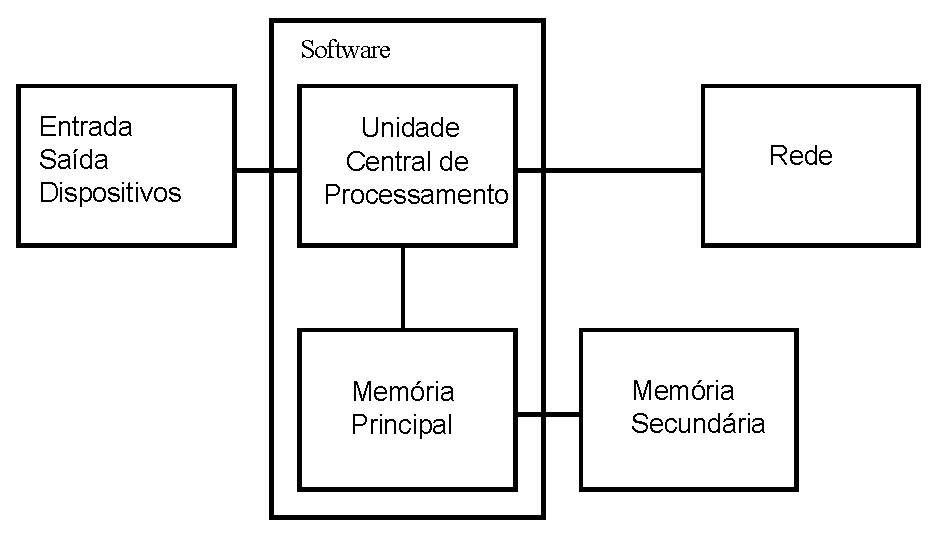
\includegraphics[height=2.50in]{figs2/arch3.eps}}
\afterfig
%\beforefig
%\centerline{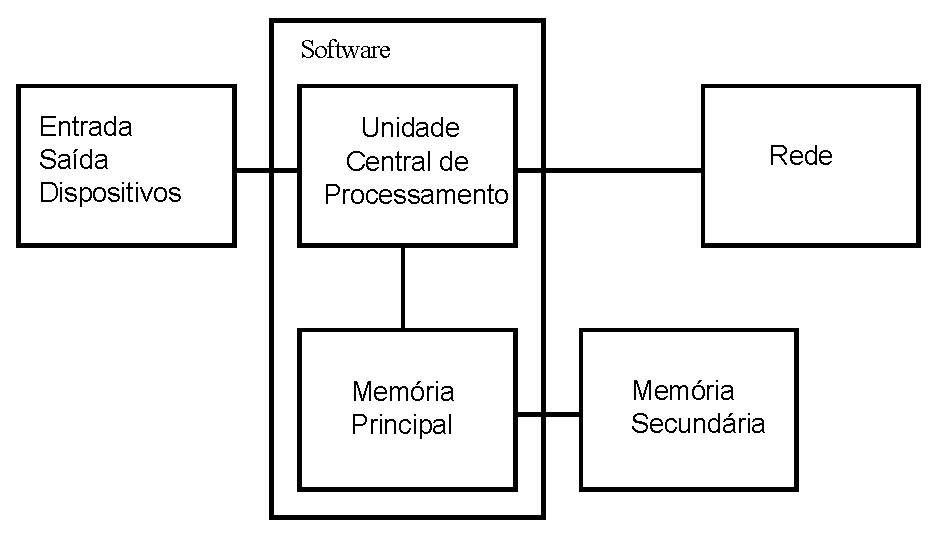
\includegraphics[height=2.50in]{figs2/arch3.eps}}
%\afterfig

Neste capítulo, começaremos a trabalhar com {\bf Memória Secundária}
(ou arquivos).
A memória secundária não é apagada quando a energia é desligada.
Ou no caso de um pen drive USB, o
dado que nós escrevemos a partir de nossos programas, pode ser
removido e transportado para outro sistema.
%In this chapter, we start to work with {\bf Secondary Memory} 
%(or files).
%Secondary memory is not erased even when the power is turned off.  
%Or in the case of a USB flash drive, the
%data we write from our programs can be removed from the 
%system and transported to another system.

Nós focaremos primeiramente na leitura e escrita de arquivos texto
tais como aqueles que criamos em um editor de texto. Depois iremos
trabalhar com arquivos de banco de dados que são arquivos binários,
especificamente desenhados para serem lidos e escritos através do nosso
software de banco de dados.
%We will primarily focus on reading and writing text files such as 
%those we create in a text editor.  Later we will see how to work
%with database files which are binary files, specifically designed to be read
%and written through database software.

\section{Lendo arquivos}
\index{arquivo!leitura}
\index{função open}
\index{função!open}
%\section{Opening files}
%\index{file!open}
%\index{open function}
%\index{function!open}

Quando queremos ler ou gravar um arquivo (nosso disco rígido, por exemplo),
devemos sempre abrir o arquivo primeiro através do comando {\bf open}. Abrir um
arquivo é uma comunicação com o seu sistema operacional, que sabe onde o dado
para cada arquivo é armazenado. Quando você abre um arquivo, você está pedindo
ao sistema operacional para encontrar o arquivo pelo nome e certificar-se de que
ele existe. Neste exemplo, abrimos o arquivo {\tt mbox.txt}, o qual deve ser armazenado
no mesmo diretório onde o seu programa Python está executando.
Você pode fazer o download deste arquivo a partir de:
\url{www.py4inf.com/code/mbox.txt}
%When we want to read or write a file (say on your hard drive), we first
%must {\bf open} the file.  Opening the file communicates with your operating
%system, which knows where the data for each file is stored.  When you open
%a file, you are asking the operating system to find the file by name
%and make sure the file exists.  In this example, we open the file 
%{\tt mbox.txt}, which should be stored in the same folder that you
%are in when you start Python.
%You can download this file from 
%\url{www.py4inf.com/code/mbox.txt}

\beforeverb
\begin{verbatim}
>>> fhand = open('mbox.txt')
>>> print fhand
<open file 'mbox.txt', mode 'r' at 0x1005088b0>
\end{verbatim}
\afterverb
%\beforeverb
%\begin{verbatim}
%>>> fhand = open('mbox.txt')
%>>> print fhand
%<open file 'mbox.txt', mode 'r' at 0x1005088b0>
%\end{verbatim}
%\afterverb
%

\index{manipulação de arquivo}
%\index{file handle}

Se o comando {\tt open} rodar com sucesso, o sistema operacional nos
retorna um {\bf manipulador de arquivo}. Este manipulador não contém
os dados do arquivo, mas apenas o ``ponteiro'' que nós podemos usar
para ler um dado. Você recebe um ponteiro se o arquivo requisitado
existir e se você tiver permissão para lê-lo.
%If the {\tt open} is successful, the operating system returns us a 
%{\bf file handle}.  The file handle is not the actual data contained
%in the file, but instead it is a ``handle'' that we can use to 
%read the data.   You are given a handle if the requested file
%exists and you have the proper permissions to read the file.

\beforefig
\centerline{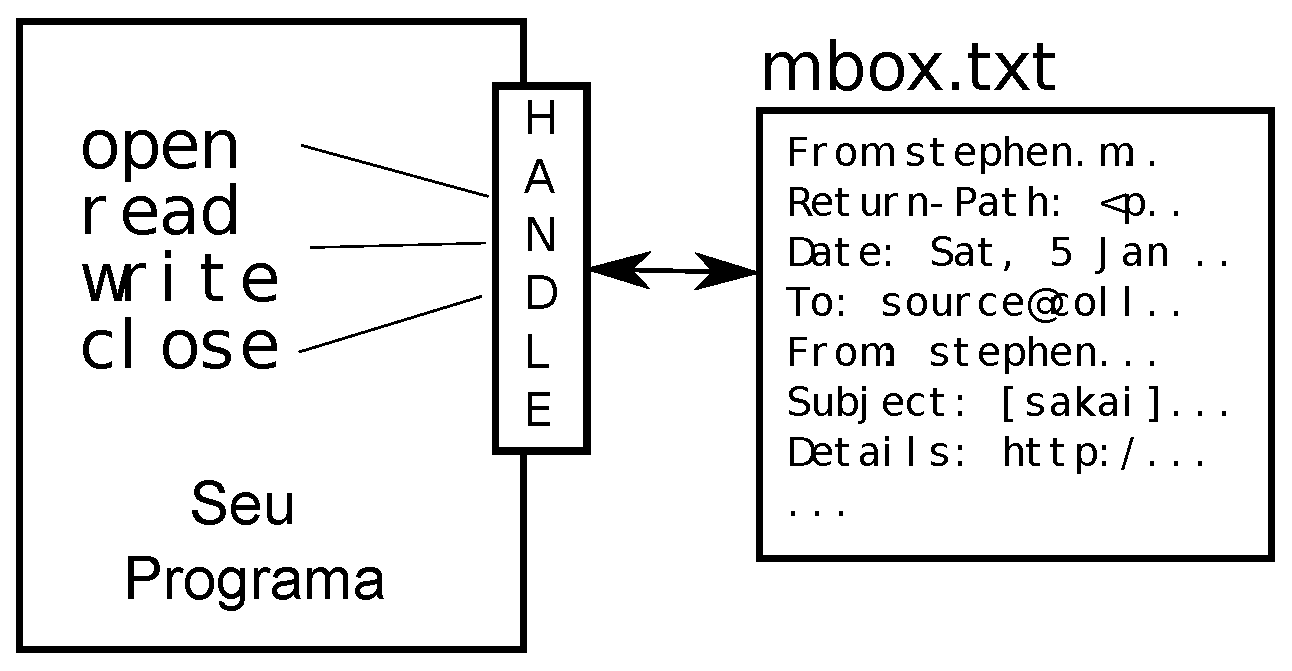
\includegraphics[height=1.75in]{figs2/handle.eps}}
\afterfig
%\beforefig
%\centerline{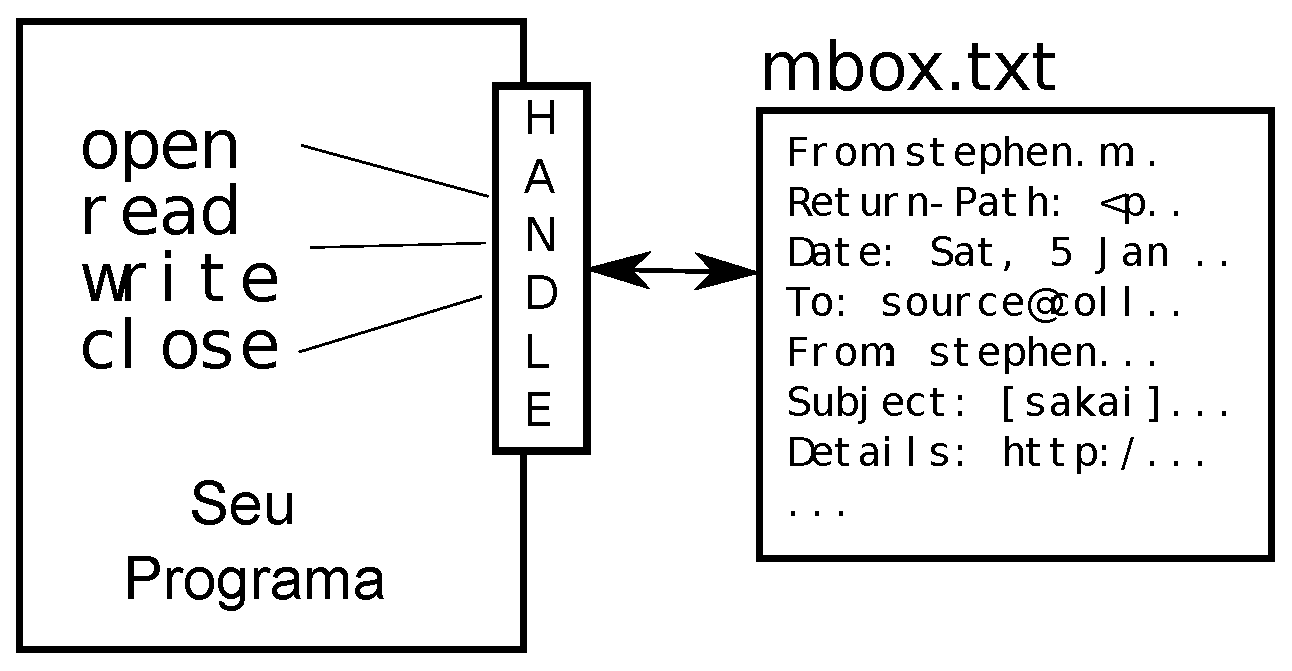
\includegraphics[height=1.75in]{figs2/handle.eps}}
%\afterfig

Se o arquivo não existir, {\tt open} ocorrerá um erro com a pilha de execução (traceback)
e você não conseguirá obter um ponteiro (handle) para acessar o conteúdo do arquivo: 
%If the file does not exist, {\tt open} will fail with a traceback and you 
%will not get a handle to access the contents of the file:

\beforeverb
\begin{verbatim}
>>> fhand = open('stuff.txt')
Traceback (most recent call last):
  File "<stdin>", line 1, in <module>
IOError: [Errno 2] No such file or directory: 'stuff.txt'
\end{verbatim}
\afterverb
%\beforeverb
%\begin{verbatim}
%>>> fhand = open('stuff.txt')
%Traceback (most recent call last):
%  File "<stdin>", line 1, in <module>
%IOError: [Errno 2] No such file or directory: 'stuff.txt'
%\end{verbatim}
%\afterverb

Mais tarde, vamos aprender a utilizar {\tt try} e {\tt except} para lidar 
com a situação onde tentamos abrir um arquivo que não existe.
%Later we will use {\tt try} and {\tt except} to deal more gracefully
%with the situation where we attempt to open a file that does 
%not exist.

\section{Arquivos texto e linhas}
%\section{Text files and lines}

Podemos imaginar um arquivo texto como um sequência de linhas, assim
como uma string em Python é uma sequência de caracteres. Por exemplo, esta
é um exemplo de um arquivo texto com registros de atividade de e-mail de várias
pessoas em um time de desenvolvimento em um projeto open source:
%A text file can be thought of as a sequence of lines, much like a Python
%string can be thought of as a sequence of characters.  For example, this
%is a sample of a text file which records mail activity from various
%individuals in an open source project development team:

\beforeverb
\begin{alltt}
From stephen.marquard@uct.ac.za Sat Jan  5 09:14:16 2008
Return-Path: <postmaster@collab.sakaiproject.org>
Date: Sat, 5 Jan 2008 09:12:18 -0500
To: source@collab.sakaiproject.org
From: stephen.marquard@uct.ac.za
Subject: [sakai] svn commit: r39772 - content/branches/
Details: http://source.sakaiproject.org/viewsvn/?view=rev\&rev=39772
...
\end{alltt}
\afterverb

O arquivo completo de iterações por e-mail está disponível em:
\url{www.py4inf.com/code/mbox.txt} 
e uma versão reduzida do arquivo está disponível em:
\url{www.py4inf.com/code/mbox-short.txt}.
Estes arquivos estão em um formato padrão de um arquivo contendo
múltiplas mensagens de e-mail. A expressão ``From '' separa as mensagens
e as linhas que começam com ``From:'' são parte da mensagem.
Para maiores informações sobre o formato mbox, veja:
\url{en.wikipedia.org/wiki/Mbox}. 
%The entire file of mail interactions is available from 
%\url{www.py4inf.com/code/mbox.txt} 
%and a shortened version of the file is available from
%\url{www.py4inf.com/code/mbox-short.txt}.
%These files are in a standard format for a file containing 
%multiple mail messages. The lines which start with 
%``From '' separate the messages and the lines which start 
%with ``From:'' are part of the messages. 
%For more information about the mbox format, see 
%\url{en.wikipedia.org/wiki/Mbox}. 

Para separar o arquivo em linhas, existe um caractere especial que
representa o ``fim da linha'' chamado de {\bf newline} caractere.
%To break the file into lines, there is a special character that 
%represents the ``end of the line'' called the {\bf newline} character.

\index{newline}
%\index{newline}

Em Python, representamos o caractere {\bf newline} como a string \textbackslash n,
uma constante string. Mesmo que essa expressão pareça ser dois caracteres, ela
é na verdade apenas um caractere simples. Quando imprimimos o valor da variável
``stuff'' no interpretador, ele nos mostra o \verb"\n" na string,
mas quando usamos {\tt print} para exibir, nós vemos uma string quebrada
em duas linhas pelo caractere newline.
%In Python, we represent the {\bf newline} character as a backslash-n in 
%string constants.  Even though this looks like two characters, it
%is actually a single character.  When we look at the variable by entering
%``stuff'' in the interpreter, it shows us the \verb"\n" in the string, 
%but when we use {\tt print} to show the string, we see the string broken
%into two lines by the newline character.

\beforeverb
\begin{verbatim}
>>> stuff = 'Hello\nWorld!'
>>> stuff
'Hello\nWorld!'
>>> print stuff
Hello
World!
>>> stuff = 'X\nY'
>>> print stuff
X
Y
>>> len(stuff)
3
\end{verbatim}
\afterverb

Você também pode ver que o tamanho da string \verb"'X\nY'" é \emph{três [three]}
caracteres porque o caractere newline é um único caractere simples.
%You can also see that the length of the string \verb"'X\nY'" is \emph{three}
%characters because the newline character is a single character.

Então, quando olhamos as linhas em um arquivo, nós precisamos \emph{imaginar}
que ele é uma espécie de caractere invisível que faz com que o fim de cada linha
seja de fato, o fim da linha.
%So when we look at the lines in a file, we need to \emph{imagine}
%that there is a special invisible character called the newline at
%the end of each line that marks the end of the line.  

 \beforeverb
 \begin{alltt}
 From stephen.marquard@uct.ac.za Sat Jan  5 09:14:16 2008\verb"\n"\\
 Return-Path: <postmaster@collab.sakaiproject.org>\verb"\n"\\
 Date: Sat, 5 Jan 2008 09:12:18 -0500\verb"\n"\\
 To: source@collab.sakaiproject.org\verb"\n"\\
 From: stephen.marquard@uct.ac.za\verb"\n"\\
 Subject: [sakai] svn commit: r39772 - content/branches/\verb"\n"\\
 Details: http://source.sakaiproject.org/viewsvn/?view=rev\&rev=39772\verb"\n"\\
 ...
 \end{alltt}
 \afterverb

Observe que o caractere newline separa os caracteres
no arquivo em linhas.
%So the newline character separates the characters 
%in the file into lines.

\section{Lendo arquivos}
%\section{Reading files}

\index{arquivo!leitura}
\index{contador}
%\index{file!reading}
%\index{counter}

O {\bf ponteiro para o arquivo} não contém o dado do arquivo,
é muito fácil construir um laço {\tt for} para ler o arquivo inteiro
e contar quantas linhas existem.
%While the {\bf file handle} does not contain the data for the file,
%it is quite easy to construct a {\tt for} loop to read through 
%and count each of the lines in a file:

\beforeverb
\begin{verbatim}
fhand = open('mbox.txt')
count = 0
for line in fhand:
    count = count + 1
print 'Line Count:', count

python open.py 
Line Count: 132045
\end{verbatim}
\afterverb

Nós podemos utilizar o ponteiro do arquivo como uma sequência no nosso
loop {\tt for}. Nosso loop {\tt for} conta o número de linhas no
arquivo e então imprime. Uma tradução grotesca do loop {\tt for} para
o português seria, ``para cada linha do arquivo representada pelo ponteiro
do arquivo, adicione um à variável {\tt count}.''
%We can use the file handle as the sequence in our {\tt for} loop.  
%Our {\tt for} loop simply counts the number of lines in the 
%file and prints them out.  The rough translation of the {\tt for}
%loop into English is, ``for each line in the file represented by the file
%handle, add one to the {\tt count} variable.''

A razão pela qual a função {\tt open} não lê o arquivo inteiro é que
o arquivo pode ser muito grande com vários gigabytes de dados.
A instrução {\tt open} recebe a mesma quantidade de tempo sem levar em
consideração o tamanho do arquivo.
%The reason that the {\tt open} function does not read the entire file
%is that the file might be quite large with many gigabytes of data.
%The {\tt open} statement takes the same amount of time regardless of the
%size of the file.  The {\tt for} loop actually causes the data to be 
%read from the file.

Quando um arquivo é lido usando um laço {\tt for} desta maneira, o Python
divide o dado do arquivo em linhas separadas pelo caractere newline.
O Python lê cada linha até encontrar o newline e então inclui o newline
como o último caractere da variável {\tt line} para cada iteração do 
laço {\tt for}. 
%When the file is read using a {\tt for} loop in this manner, Python
%takes care of splitting the data in the file into separate lines using
%the newline character.  Python reads each line through 
%the newline and includes
%the newline as the last character in the {\tt line} variable for each 
%iteration of the {\tt for} loop.

Pelo fato de o laço {\tt for} ler o dado uma linha de cada vez, ele
consegue eficientemente ler e contar as linhas em um arquivos grandes
sem estourar a memória do computador para armazenar os dados. O programa
acima pode contar as linhas em qualquer tamanho de arquivo usando pouca
quantidade de memória uma vez que cada linha é lida, contada e então
descartada. 
%Because the {\tt for} loop reads the data one line at a time, it can efficiently
%read and count the lines in very large files without running 
%out of main memory to store the data.  The above program can 
%count the lines in any size file using very little memory since 
%each line is read, counted, and then discarded.

Se você souber que o arquivo é relativamente pequeno comparado ao 
tamanho total da memória principal, você pode ler o arquivo inteiro
para uma única string usando o método {\tt read} no ponteiro do arquivo
{\tt handle}.
%If you know the file is relatively small compared to the size of 
%your main memory, you can read the whole file into one string
%using the {\tt read} method on the file handle.

\beforeverb
\begin{verbatim}
>>> fhand = open('mbox-short.txt')
>>> inp = fhand.read()
>>> print len(inp)
94626
>>> print inp[:20]
From stephen.marquar
\end{verbatim}
\afterverb

Neste exemplo, o conteúdo total (todos os 94.626 caracteres)
do arquivo {\tt mbox-short.txt} são lidos diretamente para a
variável {\tt inp}. Nós usamos o método de fatiar a string {\tt slice}
para imprimir os primeiros 20 caracteres dos dados armazenados na string
{\tt inp}.
%In this example, the entire contents (all 94,626 characters) 
%of the file {\tt mbox-short.txt} are read directly into the 
%variable {\tt inp}.  We use string slicing to print out the first
%20 characters of the string data stored in {\tt inp}.

Quando o arquivo é lido deste modo, todos os caracteres incluindo 
todas as linhas e caracteres newline são uma única e grande string
dentro da variável {\bf inp}.
Lembre que este modo de utilizar a função {\tt open} deve somente ser
usado se o tamanho do arquivo lido couber perfeitamente na memória 
principal do seu computador.
%When the file is read in this manner, all the characters including 
%all of the lines and newline characters are one big string 
%in the variable {\bf inp}.  
%Remember that this form of the {\tt open} function should only be used
%if the file data will fit comfortably in the main memory 
%of your computer.

Se o arquivo for muito grande para a memória principal, você deve
escrever seu programa para ler o arquivo em blocos, usando um laço 
{\tt for} ou {\tt while}.
%If the file is too large to fit in main memory, you should write
%your program to read the file in chunks using a {\tt for} or {\tt while}
%loop.

\section{Fazendo buscas em um arquivo}
%\section{Searching through a file}

Quando você estiver procurando algo dentro de um arquivo, esta
é uma forma comum de se percorrer todo o arquivo, ignorando a 
maioria das linhas e somente processando aquelas que atendam a uma
condição particular. Nós podemos combinar padrões para leitura em
um arquivo com os métodos da classe string para construir mecanismos 
simples de busca.
%When you are searching through data in a file, it
%is a very common pattern to read through a file, ignoring most
%of the lines and only processing lines which meet a particular condition.
%We can combine the pattern for reading a file with string methods
%to build simple search mechanisms.

\index{padrão de filtro}
\index{padrão!filtro}
%\index{filter pattern}
%\index{pattern!filter}

Por exemplo, se quisermos ler o arquivo, imprimindo apenas as linhas
que iniciarem com o prefixo ``From:'', podemos usar o método da classe 
string {\bf startswith} para selecionar apenas as linhas com o prefixo 
desejado:
%For example, if we wanted to read a file and only print out lines
%which started with the prefix ``From:'', we could use the 
%string method {\bf startswith} to select only those lines with
%the desired prefix:

\beforeverb
\begin{verbatim}
fhand = open('mbox-short.txt')
for line in fhand:
    if line.startswith('From:') :
        print line
\end{verbatim}
\afterverb

Quando este programa executa, obtemos a seguinte saída:
%When this program runs, we get the following output:

\beforeverb
\begin{verbatim}
From: stephen.marquard@uct.ac.za

From: louis@media.berkeley.edu

From: zqian@umich.edu

From: rjlowe@iupui.edu
...
\end{verbatim}
\afterverb

O programa funcionou, uma vez que a saída imprimiu apenas aquelas
linhas que iniciam com o prefixo ``From:''. Mas porque iríamos querer
as linhas em branco? Isto se deve ao caractere invisível {\bf newline}.
Cada uma das linhas terminam com um newline, então a instrução {\tt print}
imprime a string contida na variável {\bf line} o que inclui um newline
e então a instrução {\t print} adiciona \emph{outro} newline, resultando
no efeito de duplo espaço que pudemos visualizar.
%The output looks great since the only lines we are seeing are those 
%which start with ``From:'', but why are we seeing the extra blank
%lines?  This is due to that invisible {\bf newline} character.
%Each of the lines ends with a newline, so the {\tt print} 
%statement prints the string in the variable {\bf line} which includes
%a newline and then {\tt print} adds \emph{another} newline, resulting
%in the double spacing effect we see.

Nós podemos utilizar o método slicing para imprimir todos os caracteres
menos o último, mas um método mais interessante é utilizar o método 
{\bf strip} para remover o espaço em branco do lado direito da string,
como segue:
%We could use line slicing to print all but the last character, but 
%a simpler approach is to use the {\bf rstrip} method which strips
%whitespace from the right side of a string as follows:

\beforeverb
\begin{verbatim}
fhand = open('mbox-short.txt')
for line in fhand:
    line = line.rstrip()
    if line.startswith('From:') :
        print line
\end{verbatim}
\afterverb

Quando este programa executa, obtemos a seguinte saída:
%When this program runs, we get the following output:

\beforeverb
\begin{verbatim}
From: stephen.marquard@uct.ac.za
From: louis@media.berkeley.edu
From: zqian@umich.edu
From: rjlowe@iupui.edu
From: zqian@umich.edu
From: rjlowe@iupui.edu
From: cwen@iupui.edu
...
\end{verbatim}
\afterverb

Conforme seus programas de processamento de arquivo se tornam mais 
complicados, você pode estruturar seus laços com a instrução 
{\tt continue}. A ideia básica do laço de busca é que você procura
por linhas ``interessantes'' e efetivamente pula aquelas ``não interessantes''.
E então quando encontrarmos uma linha interessante, podemos fazer algo com ela.
%As your file processing programs get more complicated, you may want 
%to structure your search loops using {\tt continue}.  The basic idea 
%of the search loop is that you are looking for ``interesting'' lines
%and effectively skipping ``uninteresting'' lines.  And then when we
%find an interesting line, we do something with that line.

Podemos estruturar o laço para seguir o padrão de
pular linhas que não interessam, como segue:
%We can structure the loop to follow the
%pattern of skipping uninteresting lines as follows:

\beforeverb
\begin{verbatim}
fhand = open('mbox-short.txt')
for line in fhand:
    line = line.rstrip()
    # Skip 'uninteresting lines'
    if not line.startswith('From:') :
        continue
    # Process our 'interesting' line
    print line
\end{verbatim}
\afterverb

A saída do programa é a mesma. As linhas que não são
interessantes são aquelas que não começam com ``From:'',
as quais nós pulamos através da instrução {\tt continue}.
As linhas interessantes (i.e., aquelas que começam com ``From:'')
são processadas pelo nosso programa.
%The output of the program is the same.  In English, the 
%uninteresting lines are those which do not start 
%with ``From:'', which we skip using {\tt continue}.
%For the ``interesting'' lines (i.e., those that start with ``From:'')
%we perform the processing on those lines.

Podemos usar o método da classe string {\tt find}, para simular
uma busca de um editor de texto que procura por uma string em todas
as linhas de um arquivo onde ela aparecer, não importa a posição da
linha. A instrução {\tt find} procura pela ocorrência de uma string 
em outra, retornando o índice da posição encontrada ou -1 caso não 
encontre. Podemos escrever o seguinte laço para mostrar as linhas que
contém a string ``@uct.ac.za'' (i.e. originadas na Universidade de
Cape Town na África do Sul):
%We can use the {\tt find} string method to simulate a text editor
%search that finds lines where the search string is anywhere in the line.  
%Since {\tt find} looks for an occurrence of a string within another
%string and either returns the position of the string or -1 if the string
%was not found, we can write the following loop to show lines which
%contain the string ``@uct.ac.za'' (i.e., they come from the University 
%of Cape Town in South Africa):

\beforeverb
\begin{verbatim}
fhand = open('mbox-short.txt')
for line in fhand:
    line = line.rstrip()
    if line.find('@uct.ac.za') == -1 : 
        continue
    print line
\end{verbatim}
\afterverb

Que produz a seguinte saída:
%Which produces the following output:

\beforeverb
\begin{verbatim}
From stephen.marquard@uct.ac.za Sat Jan  5 09:14:16 2008
X-Authentication-Warning: set sender to stephen.marquard@uct.ac.za using -f
From: stephen.marquard@uct.ac.za
Author: stephen.marquard@uct.ac.za
From david.horwitz@uct.ac.za Fri Jan  4 07:02:32 2008
X-Authentication-Warning: set sender to david.horwitz@uct.ac.za using -f
From: david.horwitz@uct.ac.za
Author: david.horwitz@uct.ac.za
...
\end{verbatim}
\afterverb

\section{Deixando o usuário escolher o nome do arquivo}
%\section{Letting the user choose the file name}

Nós não queremos ter que editar nosso código Python toda vez
que tivermos que processar um arquivo diferente. É melhor
pedir que o usuário digite o nome do arquivo cada vez que
o programa executar, assim nosso programa pode ser utilizado
para executar diferentes arquivos sem ter que ficar alterando
o script Python.
%We really do not want to have to edit our Python code
%every time we want to process a different file.  It would 
%be more usable to ask the user to enter the file name string 
%each time the program runs so they can use our 
%program on different files without changing the Python code.

Isto é muito fácil de se fazer, basta utilizarmos a instrução
\verb"raw_input" como mostrado a seguir:
%This is quite simple to do by reading the file name from
%the user using \verb"raw_input" as follows:

\beforeverb
\begin{verbatim}
fname = raw_input('Enter the file name: ')
fhand = open(fname)
count = 0
for line in fhand:
    if line.startswith('Subject:') :
        count = count + 1
print 'There were', count, 'subject lines in', fname
\end{verbatim}
\afterverb

O nome do arquivo é lido através da entrada do usuário e armazenado
em uma variável chamada {\tt fname} e então o arquivo é aberto. Desta
forma podemos executar o programa diversas vezes na leitura de 
diferentes arquivos.
%We read the file name from the user and place it in a variable
%named {\tt fname} and open that file.  Now we can run the program 
%repeatedly on different files.

\beforeverb
\begin{verbatim}
python search6.py 
Enter the file name: mbox.txt
There were 1797 subject lines in mbox.txt

python search6.py 
Enter the file name: mbox-short.txt
There were 27 subject lines in mbox-short.txt
\end{verbatim}
\afterverb

Antes de espiar a próxima seção, dê uma olhada no programa acima
e pergunte a você mesmo, ``O que pode dar errado aqui?'' ou ``O que
será que o nosso amigo usuário pode querer fazer que vá fazer com que
o nosso pequeno programa terminar com um erro inesperado e um traceback,
fazendo com que olhemos de uma forma não tão bacana para os olhos dos
nossos queridos usuários?''
%Before peeking at the next section, take a look at the above program
%and ask yourself, ``What could go possibly wrong here?'' or ``What might our
%friendly user do that would cause our nice little program to 
%ungracefully exit with a traceback, making us look not-so-cool 
%in the eyes of our users?''

\section{Usando {\tt try, except,} e {\tt open}}
%\section{Using {\tt try, except,} and {\tt open}}

Eu disse para você não espiar. Esta é a sua última chance
%I told you not to peek.  This is your last chance.

O que aconteceria se o usuário digitasse qualquer outra coisa
que não fosse o nome de um arquivo?
%What if our user types something that is not a file name?

\beforeverb
\begin{verbatim}
python search6.py 
Enter the file name: missing.txt
Traceback (most recent call last):
  File "search6.py", line 2, in <module>
    fhand = open(fname)
IOError: [Errno 2] No such file or directory: 'missing.txt'

python search6.py 
Enter the file name: na na boo boo
Traceback (most recent call last):
  File "search6.py", line 2, in <module>
    fhand = open(fname)
IOError: [Errno 2] No such file or directory: 'na na boo boo'
\end{verbatim}
\afterverb

Não dê risada, os usuários tentarão de todas as formas fazer com que
o nosso programa dê erros---seja com um propósito ou com intenção
maliciosa. Na verdade, uma importante atividade de qualquer time de 
desenvolvimento de software é uma pessoa ou grupo chamado {Quality Assurance}
(ou QA), cuja principal responsabilidade é fazer as coisas mais loucas
possíveis na tentativa de quebrar o software que o programador criou.
%Do not laugh, users will eventually do every possible thing they can do 
%to break your programs---either on purpose or with malicious intent.
%As a matter of fact, an important part of any software development
%team is a person or group called {\bf Quality Assurance} (or QA for short)
%whose very job it is to do the craziest things possible in an attempt
%to break the software that the programmer has created.

\index{Quality Assurance}
\index{QA}
%\index{Quality Assurance}
%\index{QA}

O time de QA é responsável por encontrar falhas em programas antes que
ele seja entregue aos usuários finais que estão pagando o software
ou o salário dos programadores. Então, o time QA são os melhores amigos
dos desenvolvedores.
%The QA team is responsible for finding the flaws in programs before 
%we have delivered the program to the end users who may be purchasing the
%software or paying our salary to write the software.  So the QA team
%is the programmer's best friend.

\index{instrução try}
\index{instrução!try}
\index{função open}
\index{função!open}
\index{exceção!IOError}
\index{IOError}
%\index{try statement}
%\index{statement!try}
%\index{open function}
%\index{function!open}
%\index{exception!IOError}
%\index{IOError}

Então, agora que encontramos uma falha no programa, podemos consertá-lo
usando a estrutura {\tt try}/{\tt except}. Podemos assumir que a chamada 
{\tt open} pode falhar e adicionar um código de tratamento para quando
o {\tt open} falhar, como segue:
%So now that we see the flaw in the program, we can elegantly fix it using
%the {\tt try}/{\tt except} structure.  We need to assume that the {\tt open}
%call might fail and add recovery code when the {\tt open} fails
%as follows:

\beforeverb
\begin{verbatim}
fname = raw_input('Enter the file name: ')
try:
    fhand = open(fname)
except:
    print 'File cannot be opened:', fname
    exit()

count = 0
for line in fhand:
    if line.startswith('Subject:') : 
        count = count + 1
print 'There were', count, 'subject lines in', fname
\end{verbatim}
\afterverb

A função {\tt exit} faz que com o programa termine. Esta é uma
função que chamamos e que nunca retorna. Agora quando nosso usuário
(ou o time QA) digitar nomes bobos ou ruins para o nome do arquivo,
nós ``capturamos'' os erros e tratamos de uma forma adequada.
%The {\tt exit} function terminates the program.  It is a function
%that we call that never returns.  Now when our user (or 
%QA team) types in silliness or bad file names, 
%we ``catch'' them and recover gracefully:

\beforeverb
\begin{verbatim}
python search7.py
Enter the file name: mbox.txt
There were 1797 subject lines in mbox.txt

python search7.py
Enter the file name: na na boo boo
File cannot be opened: na na boo boo
\end{verbatim}
\afterverb

\index{Pythônico}
%\index{Pythonic}

Proteger a chamada da função {\tt open} é um bom
exemplo do uso correto da instrução {\tt try} e 
{\tt catch} em um programa Python. Utilizamos o termo
``Pythônico'' quando estamos fazendo do ``jeito Python''.
Podemos dizer que o exemplo acima é o jeito Pythônico
de se abrir um arquivo.
%Protecting the {\tt open} call is a good example 
%of the proper use of {\tt try}
%and {\tt except} in a Python program.  We use the term
%``Pythonic'' when we are doing something the ``Python
%way''.  We might say that the above example is 
%the Pythonic way to open a file.

Quando você se tornar mais qualificado em Python, pode
ajudar outros programadores Python a decidir qual de duas
soluções equivalentes para um determinado problema é
``mais Pythônica''. O objetivo de ser ``mais Pythônico''
remete à noção de que programação é parte da engenharia
e da arte. Não estamos interessados em apenas fazer algo
funcionar, queremos que a nossa solução seja elegante
e apreciada por nossos colegas.
%Once you become more skilled in Python, you can engage
%in repartee with other Python programmers to decide
%which of two equivalent solutions to a problem is 
%``more Pythonic''.  The goal to be ``more Pythonic'' 
%captures the notion that programming is part engineering
%and part art.  We are not always interested
%in just making something work, we also want
%our solution to be elegant and to be appreciated as 
%elegant by our peers.

\section{Escrevendo arquivos}
%\section{Writing files}

\index{arquivos!escrita}
%\index{file!writing}

Para escrever um arquivo, você deve abri-lo no
modo \verb"'w'" como segundo parâmetro.
%To write a file, you have to open it with mode
%\verb"'w'" as a second parameter:

\beforeverb
\begin{verbatim}
>>> fout = open('output.txt', 'w')
>>> print fout
<open file 'output.txt', mode 'w' at 0xb7eb2410>
\end{verbatim}
\afterverb

Se o arquivo já existir, abri-lo no modo escrita irá limpar o
conteúdo do arquivo e iniciar uma escrita limpa, então tenha 
cuidado! Se o arquivo não existir, um novo será criado.
%If the file already exists, opening it in write mode clears out
%the old data and starts fresh, so be careful!
%If the file doesn't exist, a new one is created.

O método {\tt write} de um objeto tratador ``(handle)'' de 
arquivo colocará dados dentro dele.
%The {\tt write} method of the file handle object 
%puts data into the file.

\beforeverb
\begin{verbatim}
>>> line1 = "This here's the wattle,\n"
>>> fout.write(line1)
\end{verbatim}
\afterverb

\index{newline}
%\index{newline}

Novamente, o objeto file mantém o endereço de onde o arquivo 
está, assim, se você chamar {\tt write} novamente, irá adicionar
dados ao final do arquivo.
%Again, the file object keeps track of where it is, so if
%you call {\tt write} again, it adds the new data to the end.

Devemos nos certificar de gerenciar o fim das linhas conforme
escrevemos em um arquivo, explicitamente inserindo o caractere
newline quando quisermos finalizar a linha. A instrução {\tt print}
adiciona automaticamente uma nova linha. A instrução {\tt print}
automaticamente adiciona uma nova linha, mas o método {\tt write}
não adiciona automaticamente uma nova linha.
%We must make sure to manage the ends of lines as we write
%to the file by explicitly inserting the newline character
%when we want to end a line.  The {\tt print} statement 
%automatically appends a newline, but the {\tt write} 
%method does not add the newline automatically.

\beforeverb
\begin{verbatim}
>>> line2 = 'the emblem of our land.\n'
>>> fout.write(line2)
\end{verbatim}
\afterverb

Quando você terminar de escrever, terá que fechar o arquivo
para se certificar de que o último bit de dados será escrito
fisicamente para o disco, assim a informação não será perdida
quando a energia desligar. 
%When you are done writing, you have to close the file
%to make sure that the last bit of data is physically written
%to the disk so it will not be lost if the power goes off.

\beforeverb
\begin{verbatim}
>>> fout.close()
\end{verbatim}
\afterverb

Podemos fechar os arquivos que abrirmos para leitura também,
mas podemos ser um pouco negligentes somente se estivermos
abrindo alguns poucos arquivos desde que o Python se certifique
de fechar todos os arquivos que foram abertos quando o programa
finalizar. Quando escrevermos arquivos, temos que fechar explicitamente
usando a instrução {\tt close} para não corromper o arquivo. 
%We could close the files which we open for read as well, 
%but we can be a little sloppy if we are only opening a few
%files since Python makes sure that all open files are 
%closed when the program ends.  When we are writing files, 
%we want to explicitly close the files so as to leave nothing
%to chance.

\index{método close}
\index{método!close}
%\index{close method}
%\index{method!close}

\section{Depurando ou ``Debugando''}
%\section{Debugging}

\index{debugando}
\index{espaço em branco}
%\index{debugging}
%\index{whitespace}

Quando você estiver lendo e escrevendo arquivos, você pode ter 
problemas com espaços em branco. Estes erros podem ser difíceis 
de se depurar porque espaços, tabs e novas linhas são normalmente
invisíveis:
%When you are reading and writing files, you might run into problems
%with whitespace.  These errors can be hard to debug because spaces,
%tabs, and newlines are normally invisible:

\beforeverb
\begin{verbatim}
>>> s = '1 2\t 3\n 4'
>>> print s
1 2	 3
 4
\end{verbatim}
\afterverb
 
\index{função repr}
\index{função!repr}
\index{representação de uma string}
%\index{repr function}
%\index{function!repr}
%\index{string representation}

A função padrão {\tt repr} pode ajudar. Recebe qualquer objeto como um
argumento e retorna a representação da string de um objeto. Para strings,
os espaços em branco são representados como caracteres com sequências
de \textbackslash n:
%The built-in function {\tt repr} can help.  It takes any object as an
%argument and returns a string representation of the object.  For
%strings, it represents whitespace
%characters with backslash sequences:

\beforeverb
\begin{verbatim}
>>> print repr(s)
'1 2\t 3\n 4'
\end{verbatim}
\afterverb

Isto pode ser muito interessante para depuração.
%This can be helpful for debugging.

Um outro problema que você pode ter é que diferentes sistemas
usam diferentes caracteres para indicar o fim da linha. Alguns
sistemas usam o newline, representado por \verb"\n". Outros usam
um caractere de retorno, representado por \verb"\r". Alguns usam os
dois. Se você mover-se entre estes diferentes sistemas, algumas 
inconsistências podem causar problemas.
%One other problem you might run into is that different systems
%use different characters to indicate the end of a line.  Some
%systems use a newline, represented \verb"\n".  Others use
%a return character, represented \verb"\r".  Some use both.
%If you move files between different systems, these inconsistencies
%might cause problems.

\index{caractere fim de linha}
%\index{end of line character}

Para a maioria dos sistemas, existem aplicativos para converter
de um formato para o outro. Você pode achá-los (e ler mais sobre
este assunto) em \url{wikipedia.org/wiki/Newline}. Ou, naturalmente,
você pode escrever o seu próprio aplicativo.
%For most systems, there are applications to convert from one
%format to another.  You can find them (and read more about this
%issue) at \url{wikipedia.org/wiki/Newline}.  Or, of course, you
%could write one yourself.

%% TBD - Doesn't Python take care of this for us????

\section{Glossário}
%\section{Glossary}

\begin{description}

\item[catch:] Para prevenir uma exceção de terminar um programa
usando as instruções {\tt try} e {\tt except}.
\index{catch}
%\item[catch:] To prevent an exception from terminating
%a program using the {\tt try} and {\tt except} statements.
%\index{catch}

\item[newline:] Um caractere especial utilizado em arquivos e strings
para indicar o fim de uma linha.
\index{newline}
%\item[newline:] A special character used in files and strings to indicate
%the end of a line.
%\index{newline}

\item[Pythonic:] Uma técnica que funciona elegantemente no Python.
``Usar try e except é um jeito \emph{Pythônico} de se recuperar de 
arquivos não existentes, por exemplo''.
\index{Pythonic}
%\item[Pythonic:] A technique that works elegantly in Python.
%``Using try and except is the \emph{Pythonic} way to recover from 
%missing files''.
%\index{Pythonic}

\item[Controle da Qualidade - QA:] Uma pessoa ou time focado em 
garantir todo o fluxo de qualidade de um produto de software. QA é
frequentemente envolvido nos testes de um produto afim de identificar
problemas antes que ele seja lançado.
\index{Controle de Qualidade - QA}
\index{QA}
%\item[Quality Assurance:] A person or team focused on insuring the 
%overall quality of a software product.  QA is often involved 
%in testing a product and identifying problems before the product 
%is released.
%\index{Quality Assurance}
%\index{QA}

\item[arquivo texto:] Uma sequência de caracteres armazenada em
um storage, como em um hard drive por exemplo.
storage like a hard drive.
\index{text file}
%\item[text file:] A sequence of characters stored in permanent
%storage like a hard drive.
%\index{text file}

\end{description}


\section{Exercícios}
%\section{Exercises}

\begin{ex}
Escreva um programa para ler um arquivo linha a linha e imprimir
o seu conteúdo inteiro em letra maiúscula. O resultado da execução
deve se parecer com o exemplo abaixo:
%\begin{ex}
%Write a program to read through a file and print the contents 
%of the file (line by line) all in upper case.  Executing the program 
%will look as follows:

\beforeverb
\begin{verbatim}
python shout.py
Enter a file name: mbox-short.txt
FROM STEPHEN.MARQUARD@UCT.AC.ZA SAT JAN  5 09:14:16 2008
RETURN-PATH: <POSTMASTER@COLLAB.SAKAIPROJECT.ORG>
RECEIVED: FROM MURDER (MAIL.UMICH.EDU [141.211.14.90])
	 BY FRANKENSTEIN.MAIL.UMICH.EDU (CYRUS V2.3.8) WITH LMTPA;
	 SAT, 05 JAN 2008 09:14:16 -0500
\end{verbatim}
\afterverb
%
You can download the file from
\url{www.py4inf.com/code/mbox-short.txt}
\end{ex}

\begin{ex}
Escreva um programa para perguntar o nome de um arquivo e então
ler suas linhas procurando por aquelas que se enquadram no seguinte
formato:
%\begin{ex}
%Write a program 
%to prompt for a file name, and then read through the file 
%and look for lines of the form:

\beforeverb
\begin{alltt}
X-DSPAM-Confidence: {\bf 0.8475}
\end{alltt}
\afterverb

Quando você encontrar uma linha que inicia com
``X-DSPAM-Confidence:'' destrinche a linha para extrair
o ponto flutuante dela. Conte as linhas e compute o total
de valores ``spam confidence'' que forem encontrados. Quando
você atingir o final do arquivo, imprima a porcentagem de 
``spam confidence'' encontrados.
%When you encounter a line that starts with 
%``X-DSPAM-Confidence:'' pull apart the line to extract the
%floating-point number on the line.  Count these lines and
%then compute the total of the spam confidence values from
%these lines. When you reach the end of the file, print out
%the average spam confidence.

\beforeverb
\begin{verbatim}
Digite o nome do arquivo: mbox.txt
Porcentagem de spam confidence: 0.894128046745

Digite o nome de um arquivo: mbox-short.txt
Porcentagem de spam confidence: 0.750718518519
\end{verbatim}
\afterverb
%\beforeverb
%\begin{verbatim}
%Enter the file name: mbox.txt
%Average spam confidence: 0.894128046745
%
%Enter the file name: mbox-short.txt
%Average spam confidence: 0.750718518519
%\end{verbatim}
%\afterverb

Teste seu programa utilizando os arquivos {\tt mbox.txt} e {\tt mbox-short.txt}.
\end{ex}
%Test your file on the {\tt mbox.txt} and {\tt mbox-short.txt} files.
%\end{ex}


\begin{ex}
Algumas vezes quando programadores se entediam ou querem ter um pouco
de diversão, eles adicionam um recurso escondido, que não faz mal, 
{\bf Easter Egg} aos seus programas 
(\url{en.wikipedia.org/wiki/Easter_egg_(media)}). Modifique o programa
que pergunta ao usuário pelo nome do arquivo e imprima uma mensagem
engraçada quando o usuário digitar exatamente a expressão: ``na na boo boo''.
O programa deve se comportar normalmente para todos os arquivos que existem
ou não existem. Aqui está um exemplo da execução do programa:
%\begin{ex}
%Sometimes when programmers get bored or want to have a bit of fun,
%they add a harmless {\bf Easter Egg} to their program 
%(\url{en.wikipedia.org/wiki/Easter_egg_(media)}). Modify the program
%that prompts the user for the file name so that it prints a funny
%message when the user types in the exact file name ``na na boo boo''. 
%The program should behave normally for all other files which exist
%and don't exist.  Here is a sample execution of the program:

\beforeverb
\begin{verbatim}
python egg.py 

Digite o nome do arquivo: mbox.txt
Existem 1797 linhas ``subject'' em mbox.txt

python egg.py 
Digite o nome do arquivo: missing.tyxt
File cannot be opened: missing.tyxt

python egg.py 
Digite o nome do arquivo: na na boo boo
NA NA BOO BOO PARA VOCE TAMBEM - Voceê caiu na pegadinha!
\end{verbatim}
\afterverb
%\beforeverb
%\begin{verbatim}
%python egg.py 
%Enter the file name: mbox.txt
%There were 1797 subject lines in mbox.txt

%python egg.py 
%Enter the file name: missing.tyxt
%File cannot be opened: missing.tyxt

%python egg.py 
%Enter the file name: na na boo boo
%NA NA BOO BOO TO YOU - You have been punk'd!
%\end{verbatim}
%\afterverb

Nós não estamos encorajando você a colocar Easter Eggs nos seus
programas---isto é apenas um exercício. 
%We are not encouraging you to put Easter Eggs in your 
%programs---this is just an exercise.

\end{ex}
%\end{ex}


% TODO % LaTeX source for ``Python for Informatics: Exploring Information''
% Copyright (c)  2010-  Charles R. Severance, All Rights Reserved

\chapter{Listas}
%\chapter{Lists}

\index{lista}
\index{type!lista}
%\index{list}
%\index{type!list}

\section{Uma lista é uma sequência}
%\section{A list is a sequence}

Assim como uma string, uma {\bf lista} é uma sequência de valores. Em
uma string, os valores são caracteres, já em uma lista, eles podem ser
de qualquer tipo. Os valores em uma lista são chamados de {\bf elementos}
e por vezes também chamados de {\bf itens}.

%Like a string, a {\bf list} is a sequence of values.  In a string, the
%values are characters; in a list, they can be any type.  The values in
%list are called {\bf elements} or sometimes {\bf items}.

\index{elemento}
\index{sequência}
\index{item}
%\index{element}
%\index{sequence}
%\index{item}

Existem diversas maneiras de se criar uma nova lista; a mais simples
é colocar os elementos dentro de colchetes (\verb"[" e \verb"]"):
 
%There are several ways to create a new list; the simplest is to
%enclose the elements in square brackets (\verb"[" and \verb"]"):

\beforeverb
\begin{verbatim}
[10, 20, 30, 40]
['crunchy frog', 'ram bladder', 'lark vomit']
\end{verbatim}
\afterverb
%\beforeverb
%\begin{verbatim}
%[10, 20, 30, 40]
%['crunchy frog', 'ram bladder', 'lark vomit']
%\end{verbatim}
%\afterverb
%

O primeiro exemplo é uma lista de quatro inteiros. A segunda é uma lista
de três strings. Os elementos de uma lista não precisam ter o mesmo tipo.
A lista a seguir contém uma string, um número flutuante, um inteiro e (lo!)
outra lista:
%The first example is a list of four integers.  The second is a list of
%three strings.  The elements of a list don't have to be the same type.
%The following list contains a string, a float, an integer, and
%(lo!) another list:

\beforeverb
\begin{verbatim}
['spam', 2.0, 5, [10, 20]]
\end{verbatim}
\afterverb

Uma lista dentro de outra lista é chamada de lista {\bf aninhada}.
%A list within another list is {\bf nested}.

\index{lista aninhada}
\index{lista!aninhada}
%\index{nested list}
%\index{list!nested}

Uma lista que não contenha elementos
é chamada de uma lista vazia; você pode criar uma com 
colchetes vazios, \verb"[]".
%A list that contains no elements is
%called an empty list; you can create one with empty
%brackets, \verb"[]".

\index{lista vazia}
\index{lista!vazia}
%\index{empty list}
%\index{list!empty}

Como você deve imaginar, você pode atribuir valores de uma lista para variáveis:
%As you might expect, you can assign list values to variables:

\beforeverb
\begin{verbatim}
>>> cheeses = ['Cheddar', 'Edam', 'Gouda']
>>> numbers = [17, 123]
>>> empty = []
>>> print cheeses, numbers, empty
['Cheddar', 'Edam', 'Gouda'] [17, 123] []
\end{verbatim}
\afterverb
%\beforeverb
%\begin{verbatim}
%>>> cheeses = ['Cheddar', 'Edam', 'Gouda']
%>>> numbers = [17, 123]
%>>> empty = []
%>>> print cheeses, numbers, empty
%['Cheddar', 'Edam', 'Gouda'] [17, 123] []
%\end{verbatim}
%\afterverb
%

\index{tarefa}
%\index{assignment}

\section{Listas são mutáveis}
%\section{Lists are mutable}

\index{lista!elemento}
\index{acesso}
\index{índice}
\index{operador colchetes}
\index{operador!colchetes}
%\index{list!element}
%\index{access}
%\index{index}
%\index{bracket operator}
%\index{operator!bracket}

A sintaxe para acessar os elementos de uma lista é a mesma utilizada
para acessar os caracteres de de uma string---o operador colchetes.
A expressão dentro dos colchetes especifica o índice. Lembre que os 
índices iniciam no 0:
%The syntax for accessing the elements of a list is the same as for
%accessing the characters of a string---the bracket operator.  The
%expression inside the brackets specifies the index.  Remember that the
%índices start at 0:

\beforeverb
\begin{verbatim}
>>> print cheeses[0]
Cheddar
\end{verbatim}
\afterverb
%
%\beforeverb
%\begin{verbatim}
%>>> print cheeses[0]
%Cheddar
%\end{verbatim}
%\afterverb

Diferente das strings, listas são mutáveis pois é possível modificar a 
ordem dos itens em uma lista ou reatribuir um item da lista.
Quando um operador colchete aparece ao lado esquerdo da atribuição, 
ele identifica o elemento da lista que será atribuído.
%Unlike strings, lists are mutable because you can change the order 
%of items in a list or reassign an item in a list.  
%When the bracket operator appears on the left side of an assignment, 
%it identifies the element of the list that will be assigned.
%

\index{mutabilidade}
%\index{mutability}

\beforeverb
\begin{verbatim}
>>> numbers = [17, 123]
>>> numbers[1] = 5
>>> print numbers
[17, 5]
\end{verbatim}
\afterverb
%\beforeverb
%\begin{verbatim}
%>>> numbers = [17, 123]
%>>> numbers[1] = 5
%>>> print numbers
%[17, 5]
%\end{verbatim}
%\afterverb
%

O element 1 de {\tt numbers}, que era 123, agora é 5.
%The one-eth element of {\tt numbers}, which
%used to be 123, is now 5.

\index{índice!inicia no zero}
\index{zero, índice inicia no}
%\index{index!starting at zero}
%\index{zero, index starting at}

Você pode pensar em uma lista como um relacionamento entre índices e
elementos. Este relacionamento é chamado de {\bf mapeamento}; cada
índice ``mapeia para'' um dos elementos.
%You can think of a list as a relationship between índices and
%elements.  This relationship is called a {\bf mapping}; each index
%``maps to'' one of the elements.  

\index{item atribuição}
\index{atribuição!item}
%\index{item assignment}
%\index{assignment!item}

índices de lista funcionam da mesma maneira que os índices de strings:
%List índices work the same way as string índices:

\begin{itemize}

\item Qualquer expressão de um inteiro pode ser usada como um índice.
%\item Any integer expression can be used as an index.

\item Se você tentar ler ou escrever um elemento que não existe, você
terá um {\tt IndexError}.
%\item If you try to read or write an element that does not exist, you
%get an {\tt IndexError}.

\index{exception!IndexError}
\index{IndexError}
%\index{exception!IndexError}
%\index{IndexError}

\item Caso um índice tenha um valor negativo, ele contará ao contrário,
do fim para o início da lista.
%\item If an index has a negative value, it counts backward from the
%end of the list.

\end{itemize}

\index{lista!índice}
%\index{list!index}

\index{lista!membros}
\index{membros!lista}
\index{operador in}
\index{operador!in}
%\index{list!membership}
%\index{membership!list}
%\index{in operator}
%\index{operator!in}

O operador {\tt in} também funciona em listas.
%The {\tt in} operator also works on lists.

\beforeverb
\begin{verbatim}
>>> cheeses = ['Cheddar', 'Edam', 'Gouda']
>>> 'Edam' in cheeses
True
>>> 'Brie' in cheeses
False
\end{verbatim}
\afterverb
%\beforeverb
%\begin{verbatim}
%>>> cheeses = ['Cheddar', 'Edam', 'Gouda']
%>>> 'Edam' in cheeses
%True
%>>> 'Brie' in cheeses
%False
%\end{verbatim}
%\afterverb

\section{Percorrendo uma lista}
\index{lista!percorrendo}
\index{percorrendo!lista}
\index{for laço}
\index{laço!for}
\index{instrução!for}
%\section{Traversing a list}
%\index{list!traversal}
%\index{traversal!list}
%\index{for loop}
%\index{loop!for}
%\index{statement!for}

A maneira mais comum de se percorrer os elementos de uma lista é
com um laço {\tt for}. A sintaxe é a mesma da utilizada para strings:
%The most common way to traverse the elements of a list is
%with a {\tt for} loop.  The syntax is the same as for strings:

\beforeverb
\begin{verbatim}
for cheese in cheeses:
    print cheese
\end{verbatim}
\afterverb
%\beforeverb
%\begin{verbatim}
%for cheese in cheeses:
%    print cheese
%\end{verbatim}
%\afterverb
%

Isto funciona se você precisa ler apenas os elementos da lista.
Porém, caso você precise escrever ou atualizar elementos, você
precisa de índices. Um forma comum de fazer isto é combinar as
funções {\tt range} e {\tt len}:
%This works well if you only need to read the elements of the
%list.  But if you want to write or update the elements, you
%need the índices.  A common way to do that is to combine
%the functions {\tt range} and {\tt len}:

\index{fazer laços!com índices}
\index{índice!fazer laços com}
%\index{looping!with índices}
%\index{index!looping with}

\beforeverb
\begin{verbatim}
for i in range(len(numbers)):
    numbers[i] = numbers[i] * 2
\end{verbatim}
\afterverb
%\beforeverb
%\begin{verbatim}
%for i in range(len(numbers)):
%    numbers[i] = numbers[i] * 2
%\end{verbatim}
%\afterverb
%

Este laço percorre a lista e atualiza cada elemento. {\tt len}
retorna o número de elementos na lista. {\tt range} retorna uma
lista de índices de 0 a $n-1$, onde $n$ é o tamanho da lista.
Cada vez que passa pelo laço, {\tt i} recebe o índice do próximo
elemento. A instrução de atribuição no corpo, 
utiliza {\tt i} para ler o valor antigo do elemento e atribuir ao novo valor.
%This loop traverses the list and updates each element.  {\tt len}
%returns the number of elements in the list.  {\tt range} returns
%a list of índices from 0 to $n-1$, where $n$ is the length of
%the list.  Each time through the loop, {\tt i} gets the index
%of the next element.  The assignment statement in the body uses
%{\tt i} to read the old value of the element and to assign the
%new value.

\index{atualizar item}
\index{atualizar!item}
%\index{item update}
%\index{update!item}

Um laço {\tt for} em uma lista vazia nunca executa as instruções dentro do laço:
%A {\tt for} loop over an empty list never executes the body:

\beforeverb
\begin{verbatim}
for x in empty:
    print 'Esta linha nunca será executada.'
\end{verbatim}
\afterverb
%\beforeverb
%\begin{verbatim}
%for x in empty:
%    print 'This never happens.'
%\end{verbatim}
%\afterverb
%

Embora uma lista possa conter outra lista, a lista aninhada ainda conta
como um único elemento. O tamanho dessa lista é quatro:
%Although a list can contain another list, the nested
%list still counts as a single element.  The length of this list is
%four:

\index{lista aninhada}
\index{aninhada!lista}
%\index{nested list}
%\index{list!nested}

\beforeverb
\begin{verbatim}
['spam', 1, ['Brie', 'Roquefort', 'Pol le Veq'], [1, 2, 3]]
\end{verbatim}
\afterverb
%\beforeverb
%\begin{verbatim}
%['spam', 1, ['Brie', 'Roquefort', 'Pol le Veq'], [1, 2, 3]]
%\end{verbatim}
%\afterverb

\section{Operações de Lista}
\index{lista!operações de}
%\section{List operations}
%\index{list!operation}

O operador {\tt +} concatena listas:
%The {\tt +} operator concatenates lists:

\index{lista!concatenação}
\index{concatenação!lista}
%\index{concatenation!list}
%\index{list!concatenation}

\beforeverb
\begin{verbatim}
>>> a = [1, 2, 3]
>>> b = [4, 5, 6]
>>> c = a + b
>>> print c
[1, 2, 3, 4, 5, 6]
\end{verbatim}
\afterverb
%\beforeverb
%\begin{verbatim}
%>>> a = [1, 2, 3]
%>>> b = [4, 5, 6]
%>>> c = a + b
%>>> print c
%[1, 2, 3, 4, 5, 6]
%\end{verbatim}
%\afterverb
%

De modo parecido, o operador {\tt *} repete uma lista pelo número de vezes informado:
%Similarly, the {\tt *} operator repeats a list a given number of times:

\index{lista!repetição}
\index{repetição!lista}
%\index{repetition!list}
%\index{list!repetition}

\beforeverb
\begin{verbatim}
>>> [0] * 4
[0, 0, 0, 0]
>>> [1, 2, 3] * 3
[1, 2, 3, 1, 2, 3, 1, 2, 3]
\end{verbatim}
\afterverb
%\beforeverb
%\begin{verbatim}
%>>> [0] * 4
%[0, 0, 0, 0]
%>>> [1, 2, 3] * 3
%[1, 2, 3, 1, 2, 3, 1, 2, 3]
%\end{verbatim}
%\afterverb
%

O primeiro exemplo repete {\tt [0]} quatro vezes. O segundo exemplo
repete a lista {\tt [1, 2, 3]} três vezes.
%The first example repeats {\tt [0]} four times.  The second example
%repeats the list {\tt [1, 2, 3]} three times.

\section{Fatiamento de Lista}
%\section{List slices}

\index{operador de fatiamento}
\index{operador de!fatiamento}
\index{índice!fatia}
\index{lista!fatia}
\index{fatia!lista}
%\index{slice operator}
%\index{operator!slice}
%\index{index!slice}
%\index{list!slice}
%\index{slice!list}

O operador de fatiamento também funciona em listas:
%The slice operator also works on lists:

\beforeverb
\begin{verbatim}
>>> t = ['a', 'b', 'c', 'd', 'e', 'f']
>>> t[1:3]
['b', 'c']
>>> t[:4]
['a', 'b', 'c', 'd']
>>> t[3:]
['d', 'e', 'f']
\end{verbatim}
\afterverb
%\beforeverb
%\begin{verbatim}
%>>> t = ['a', 'b', 'c', 'd', 'e', 'f']
%>>> t[1:3]
%['b', 'c']
%>>> t[:4]
%['a', 'b', 'c', 'd']
%>>> t[3:]
%['d', 'e', 'f']
%\end{verbatim}
%\afterverb
%

Se você omite o primeiro índice, o fatiamento é iniciado no começo da lista.
Se omitir o segundo, o fatiamento vai até fim. Então se ambos são omitidos,
a fatia é uma cópia da lista inteira.
%If you omit the first index, the slice starts at the beginning.
%If you omit the second, the slice goes to the end.  So if you
%omit both, the slice is a copy of the whole list.

\index{lista!cópia}
\index{fatia!cópia}
\index{cópia!fatia}
%\index{list!copy}
%\index{slice!copy}
%\index{copy!slice}

\beforeverb
\begin{verbatim}
>>> t[:]
['a', 'b', 'c', 'd', 'e', 'f']
\end{verbatim}
\afterverb
%\beforeverb
%\begin{verbatim}
%>>> t[:]
%['a', 'b', 'c', 'd', 'e', 'f']
%\end{verbatim}
%\afterverb
%

Uma vez que lista são mutáveis, com frequência é útil fazer uma cópia
antes de realizar operações que dobram, reviram ou mutilam listas.
%Since lists are mutable, it is often useful to make a copy
%before performing operations that fold, spindle, or mutilate
%lists.

\index{mutabilidade}
%\index{mutability}

Um operador de fatiamento do lado esquerdo de uma atribuição pode atualizar múltiplos elementos.
%A slice operator on the left side of an assignment
%can update multiple elements:

\index{fatia!atualização}
\index{atualização!fatia}
%\index{slice!update}
%\index{update!slice}

\beforeverb
\begin{verbatim}
>>> t = ['a', 'b', 'c', 'd', 'e', 'f']
>>> t[1:3] = ['x', 'y']
>>> print t
['a', 'x', 'y', 'd', 'e', 'f']
\end{verbatim}
\afterverb
%\beforeverb
%\begin{verbatim}
%>>> t = ['a', 'b', 'c', 'd', 'e', 'f']
%>>> t[1:3] = ['x', 'y']
%>>> print t
%['a', 'x', 'y', 'd', 'e', 'f']
%\end{verbatim}
%\afterverb
%

\section{Métodos de lista}
%\section{List methods}

\index{lista!método}
\index{método, lista}
%\index{list!method}
%\index{method, list}

O Python provê métodos que operam nas listas. Por exemplo,
{\tt append} adiciona um novo elemento ao fim da lista:
%Python provides methods that operate on lists.  For example,
%{\tt append} adds a new element to the end of a list:

\index{método append}
\index{método!append}
%\index{append method}
%\index{method!append}

\beforeverb
\begin{verbatim}
>>> t = ['a', 'b', 'c']
>>> t.append('d')
>>> print t
['a', 'b', 'c', 'd']
\end{verbatim}
\afterverb
%\beforeverb
%\begin{verbatim}
%>>> t = ['a', 'b', 'c']
%>>> t.append('d')
%>>> print t
%['a', 'b', 'c', 'd']
%\end{verbatim}
%\afterverb
%

{\tt extend} recebe uma lista como argumento e adiciona todos seus elementos.
%{\tt extend} takes a list as an argument and appends all of
%the elements:

\index{método extender}
\index{extender!método}
%\index{extend method}
%\index{method!extend}

\beforeverb
\begin{verbatim}
>>> t1 = ['a', 'b', 'c']
>>> t2 = ['d', 'e']
>>> t1.extend(t2)
>>> print t1
['a', 'b', 'c', 'd', 'e']
\end{verbatim}
\afterverb
%\beforeverb
%\begin{verbatim}
%>>> t1 = ['a', 'b', 'c']
%>>> t2 = ['d', 'e']
%>>> t1.extend(t2)
%>>> print t1
%['a', 'b', 'c', 'd', 'e']
%\end{verbatim}
%\afterverb
%

Este exemplo deixa {\tt t2} sem modificação.
%This example leaves {\tt t2} unmodified.

{\tt sort} organiza os elementos da lista do menor para o maior:
%{\tt sort} arranges the elements of the list from low to high:

\index{método sort}
\index{sort!método}
%\index{sort method}
%\index{method!sort}

\beforeverb
\begin{verbatim}
>>> t = ['d', 'c', 'e', 'b', 'a']
>>> t.sort()
>>> print t
['a', 'b', 'c', 'd', 'e']
\end{verbatim}
\afterverb
%\beforeverb
%\begin{verbatim}
%>>> t = ['d', 'c', 'e', 'b', 'a']
%>>> t.sort()
%>>> print t
%['a', 'b', 'c', 'd', 'e']
%\end{verbatim}
%\afterverb
%

A maior parte dos métodos de lista são vazios; eles modificam a lista e retornam {\tt None}.
Caso você acidentalmente escreva {\tt t = t.sort()}, ficará desapontado com o resultado.
%Most list methods are void; they modify the list and return {\tt None}.
%If you accidentally write {\tt t = t.sort()}, you will be disappointed
%with the result.

\index{método void}
\index{método!void}
\index{None valor especial}
\index{valor especial!None}
%\index{void method}
%\index{method!void}
%\index{None special value}
%\index{special value!None}

\section{Deletando elementos}
%\section{Deleting elements}

\index{deleção de elemento}
\index{deleção, elemento de uma lista}
%\index{element deletion}
%\index{deletion, element of list}

Existem diversas maneiras de se deletar elementos de uma lista. Se você
souber o índice do elemento que você quer, pode usar o {\tt pop}:
%There are several ways to delete elements from a list.  If you
%know the index of the element you want, you can use
%{\tt pop}:

\index{método pop}
\index{método!pop}
%\index{pop method}
%\index{method!pop}

\beforeverb
\begin{verbatim}
>>> t = ['a', 'b', 'c']
>>> x = t.pop(1)
>>> print t
['a', 'c']
>>> print x
b
\end{verbatim}
\afterverb
%\beforeverb
%\begin{verbatim}
%>>> t = ['a', 'b', 'c']
%>>> x = t.pop(1)
%>>> print t
%['a', 'c']
%>>> print x
%b
%\end{verbatim}
%\afterverb
%

{\tt pop} modifica a lista e retorna o elemento que foi removido.
Se você não informa um índice, ele deletará e retornará o último elemento da lista.
%{\tt pop} modifies the list and returns the element that was removed.
%If you don't provide an index, it deletes and returns the
%last element.

Se você não precisa do valor removido, poderá usar o operador {\tt del}:
%If you don't need the removed value, you can use the {\tt del}
%operator:

\index{operador del}
\index{operador!del}
%\index{del operator}
%\index{operator!del}

\beforeverb
\begin{verbatim}
>>> t = ['a', 'b', 'c']
>>> del t[1]
>>> print t
['a', 'c']
\end{verbatim}
\afterverb
%\beforeverb
%\begin{verbatim}
%>>> t = ['a', 'b', 'c']
%>>> del t[1]
%>>> print t
%['a', 'c']
%\end{verbatim}
%\afterverb
%

Se você sabe qual elemento você quer remover ( mas não sabe o índice ), você
pode usar o {\tt remove}:
%If you know the element you want to remove (but not the index), you
%can use {\tt remove}:

\index{método remove}
\index{método!remove}
%\index{remove method}
%\index{method!remove}

\beforeverb
\begin{verbatim}
>>> t = ['a', 'b', 'c']
>>> t.remove('b')
>>> print t
['a', 'c']
\end{verbatim}
\afterverb
%
O valor retornado de {\tt remove} é {\tt None}.
%The return value from {\tt remove} is {\tt None}.

\index{valor especial None}
\index{valor especial!None}

Para remover mais de um elemento, você pode usar {\tt del} com 
um índice de fatiamento:
%To remove more than one element, you can use {\tt del} with
%a slice index:

\beforeverb
\begin{verbatim}
>>> t = ['a', 'b', 'c', 'd', 'e', 'f']
>>> del t[1:5]
>>> print t
['a', 'f']
\end{verbatim}
\afterverb
%\beforeverb
%\begin{verbatim}
%>>> t = ['a', 'b', 'c']
%>>> t.remove('b')
%>>> print t
%['a', 'c']
%\end{verbatim}
%\afterverb
%

Como de costume, uma fatia seleciona todos os elementos até o segundo índice, porém sem incluí-lo.
%As usual, the slice selects all the elements up to, but not
%including, the second index.

\section{Listas e funções}
%\section{Lists and functions}

Existem várias funções built-in que podem ser usadas em listas,
permitindo que você tenha uma visão rápida da lista sem a necessidade de escrever 
o seu próprio laço:
%There are a number of built-in functions that can be used on lists
%that allow you to quickly look through a list without
%writing your own loops:

\beforeverb
\begin{verbatim}
>>> nums = [3, 41, 12, 9, 74, 15]
>>> print len(nums)
6
>>> print max(nums)
74
>>> print min(nums)
3
>>> print sum(nums)
154
>>> print sum(nums)/len(nums)
25
\end{verbatim}
\afterverb
%\beforeverb
%\begin{verbatim}
%>>> nums = [3, 41, 12, 9, 74, 15]
%>>> print len(nums)
%6
%>>> print max(nums)
%74
%>>> print min(nums)
%3
%>>> print sum(nums)
%154
%>>> print sum(nums)/len(nums)
%25
%\end{verbatim}
%\afterverb
%

A função {\tt sum()} funciona apenas quando os elementos da lista são números.
As outras funções ({\tt max()}, {\tt len()}, etc.) funcionam com listas de strings
e outros tipos que são comparáveis.
%The {\tt sum()} function only works when the list elements are numbers.
%The other functions ({\tt max()}, {\tt len()}, etc.) work with lists of
%strings and other types that can be comparable.

Nós podemos reescrever um programa anterior que computou a média de uma lista de 
números adicionados pelo usuário utilizando uma lista.
%We could rewrite an earlier program that computed the average of 
%a list of numbers entered by the user using a list.

Primeiramente, o programa para calcular uma média sem uma lista:
%First, the program to compute an average without a list:

\beforeverb
\begin{verbatim}
total = 0
count = 0
while ( True ) :
    inp = raw_input('Digite um número: ')
    if inp == 'done' : break
    value = float(inp)
    total = total + value
    count = count + 1

average = total / count
print 'Average:', average
\end{verbatim}
\afterverb
%\beforeverb
%\begin{verbatim}
%total = 0
%count = 0
%while ( True ) :
%    inp = raw_input('Enter a number: ')
%    if inp == 'done' : break
%    value = float(inp)
%    total = total + value
%    count = count + 1
%
%average = total / count
%print 'Average:', average
%\end{verbatim}
%\afterverb
%

Neste programa, temos as variáveis {\tt count} e {\tt total} para armazenar
a contagem e o total da soma dos número que o usuário digitou, enquanto pedimos 
mais números para o usuário.
% In this program, we have {\tt count} and {\tt total} variables to 
% keep the number and running total of the user's numbers as 
% we repeatedly prompt the user for a number.

Nós poderíamos simplesmente guardar cada número a medida que o usuário vai 
adicionando e usar funções built-in para calcular a soma e a contagem no final.
%We could simply remember each number as the user entered it 
%and use built-in functions to compute the sum and count at
%the end.

\beforeverb
\begin{verbatim}
numlist = list()
while ( True ) :
    inp = raw_input('Digite um número: ')
    if inp == 'done' : break
    value = float(inp)
    numlist.append(value)

average = sum(numlist) / len(numlist)
print 'Média:', average
\end{verbatim}
\afterverb
%\beforeverb
%\begin{verbatim}
%numlist = list()
%while ( True ) :
%    inp = raw_input('Enter a number: ')
%    if inp == 'done' : break
%    value = float(inp)
%    numlist.append(value)
%
%average = sum(numlist) / len(numlist)
%print 'Average:', average
%\end{verbatim}
%\afterverb
%

Nós criamos uma lista vazia antes do loop iniciar, e então sempre que tivermos
um número, este será adicionado na lista. Ao final do programa, calcularemos
a soma dos números da lista e dividiremos o total pela contagem de números na lista para chegar
a média.
% We make an empty list before the loop starts, and then each time we have 
% a number, we append it to the list.  At the end of
% the program, we simply compute the sum of the numbers in the 
% list and divide it by the count of the numbers in the
% list to come up with the average.

\section{Listas e strings}
%\section{Lists and strings}

\index{lista}
\index{string}
\index{sequência}
%\index{list}
%\index{string}
%\index{sequence}

Uma string é uma sequência de caracteres e uma lista é uma sequência de valores,
porém, uma lista de caracteres não é o mesmo que uma string. Para converter uma
string para lista de caracteres você pode usar {\tt list}:
% A string is a sequence of characters and a list is a sequence
% of values, but a list of characters is not the same as a
% string.  To convert from a string to a list of characters,
% you can use {\tt list}:

\index{list!function}
\index{function!list}
%\index{list!function}
%\index{function!list}

\beforeverb
\begin{verbatim}
>>> s = 'spam'
>>> t = list(s)
>>> print t
['s', 'p', 'a', 'm']
\end{verbatim}
\afterverb
%\beforeverb
%\begin{verbatim}
%>>> s = 'spam'
%>>> t = list(s)
%>>> print t
%['s', 'p', 'a', 'm']
%\end{verbatim}
%\afterverb
%

Em razão de {\tt list} ser o nome de uma função built-in, você deve evitar
usar isto como nome de variável. Eu também evito a letra {\tt l} pois se parece muito
com o número {\tt 1}. Por essa razão utilizo {\tt t}.
% Because {\tt list} is the name of a built-in function, you should
% avoid using it as a variable name.  I also avoid the letter {\tt l} because
% it looks too much like the number {\tt 1}.  So that's why I use {\tt t}.

A função {\tt list} quebra uma string em letras individuais. Se você deseja quebrar
uma string em palavras, você deve usar o método {\tt split}.
% The {\tt list} function breaks a string into individual letters.  If
% you want to break a string into words, you can use the {\tt split}
% method:

\index{método split}
\index{método!split}
%\index{split method}
%\index{method!split}

\beforeverb
\begin{verbatim}
>>> s = 'pining for the fjords'
>>> t = s.split()
>>> print t
['pining', 'for', 'the', 'fjords']
>>> print t[2]
the
\end{verbatim}
\afterverb
%\beforeverb
%\begin{verbatim}
%>>> s = 'pining for the fjords'
%>>> t = s.split()
%>>> print t
%['pining', 'for', 'the', 'fjords']
%>>> print t[2]
%the
%\end{verbatim}
%\afterverb
%

Uma vez que você usou {\tt split} para quebrar uma string em uma lista
de palavras, você pode usar o operador de índice (colochete) para ver
uma palavra em particular dentro da lista.
% Once you have used {\tt split} to break the string into 
% a list of words, you can use the index operator (square
% bracket) to look at a particular word in the list.

Você pode chamar {\tt split} com um argumento opcional chamado {\bf delimitador}
que especifica quais caracteres a serem usados como delimitadores de palavra.
O exemplo a seguir usa um hífen como delimitador:
% You can call {\tt split} with 
% an optional argument called a {\bf delimiter} that 
% specifies which characters to use as word boundaries.
% The following example uses a hyphen as a delimiter:

\index{argumento opcional}
\index{opcional!argumento}
\index{delimitador}
%\index{optional argument}
%\index{argument!optional}
%\index{delimiter}

\beforeverb
\begin{verbatim}
>>> s = 'spam-spam-spam'
>>> delimiter = '-'
>>> s.split(delimiter)
['spam', 'spam', 'spam']
\end{verbatim}
\afterverb
%\beforeverb
%\begin{verbatim}
%>>> s = 'spam-spam-spam'
%>>> delimiter = '-'
%>>> s.split(delimiter)
%['spam', 'spam', 'spam']
%\end{verbatim}
%\afterverb
%

{\tt join} é o inverso de {\tt split}. Ele recebe uma lista de strings e
concatena seus elementos. {\tt join} é um método da classe string, então você pode invocá-lo
no delimitador e passar a lista como parâmetro.
% {\tt join} is the inverse of {\tt split}.  It
% takes a list of strings and
% concatenates the elements.  {\tt join} is a string method,
% so you have to invoke it on the delimiter and pass the
% list as a parameter:

\index{metódo join}
\index{método!join}
\index{concatenação}
%\index{join method}
%\index{method!join}
%\index{concatenation}

\beforeverb
\begin{verbatim}
>>> t = ['pining', 'for', 'the', 'fjords']
>>> delimiter = ' '
>>> delimiter.join(t)
'pining for the fjords'
\end{verbatim}
\afterverb
%\beforeverb
%\begin{verbatim}
%>>> t = ['pining', 'for', 'the', 'fjords']
%>>> delimiter = ' '
%>>> delimiter.join(t)
%'pining for the fjords'
%\end{verbatim}
%\afterverb
%

Neste caso, o delimitador é um caractere espaço, então
{\tt join} coloca um espaço entre as palavras. Para concatenar
strings sem espaços você pode usar uma string vazia, \verb"''",
como delimitador.
% In this case the delimiter is a space character, so
% {\tt join} puts a space between words.  To concatenate
% strings without spaces, you can use the empty string,
% \verb"''", as a delimiter. 

\index{string vazia}
\index{vazia!string}
%\index{empty string}
%\index{string!empty}

\section{Analisando linhas de um texto}
%\section{Parsing lines}

Normalmente quando estamos lendo um arquivo,
queremos fazer algo com as linhas e não somente
imprimir a linha inteira. Frequentemente queremos 
encontrar as ``linhas interessantes'' e então {\bf analisar}
a linha para encontrar a \emph{parte} interessante da linha.
E se quiséssemos imprimir o dia da semana das linhas que começam com
``From ''?
% Usually when we are reading a file 
% we want to do something to the lines other than just 
% printing the whole line.  Often we want to find the ``interesting
% lines'' and then {\bf parse} the line to find some interesting
% \emph{part} of the line.  What if we wanted to print out the day of the 
% week from those lines that start with ``From ''?

\beforeverb
\begin{alltt}
From stephen.marquard@uct.ac.za {\bf Sat} Jan  5 09:14:16 2008
\end{alltt}
\afterverb

O método {\tt split} é muito efetivo quando temos este tipo de 
problema.
Podemos escrever um pequeno programa que procure por linhas onde
a linha inicia com ``From '', dividir essas linhas, e então imprimir
a terceira palavra da linha:
% The {\tt split} method is very effective when faced with this 
% kind of problem.
% We can write a small program that looks for lines where the 
% line starts with ``From '', {\tt split} those lines, 
% and then print out the third word in the line:

\beforeverb
\begin{verbatim}
fhand = open('mbox-short.txt')
for line in fhand:
    line = line.rstrip()
    if not line.startswith('From ') : continue
    words = line.split()
    print words[2]
\end{verbatim}
\afterverb
%\beforeverb
%\begin{verbatim}
%fhand = open('mbox-short.txt')
%for line in fhand:
%    line = line.rstrip()
%    if not line.startswith('From ') : continue
%    words = line.split()
%    print words[2]
%\end{verbatim}
%\afterverb
%

Aqui também utilizamos o {\tt if} de forma contraída
onde colocamos o {\tt continue } na mesma linha
do {\tt if}. A forma contraída do {\tt if} funciona
da mesma maneira que funcionaria se o {\tt continue}
estivesse na próxima linha e indentado.
% Here we also use the contracted form of the {\tt if}
% statement where we put the {\tt continue } on the
% same line as the {\tt if}.  This contracted form
% of the {\tt if} functions the same as if the
% {\tt continue} were on the next line and indented.

O programa produz a saída a seguir:
% The program produces the following output:

\beforeverb
\begin{verbatim}
Sat
Fri
Fri
Fri
    ...
\end{verbatim}
\afterverb
%

Futuramente, iremos aprender técnicas cada vez mais sofisticadas
para pegar as linhas e como separar essas linhas para encontrar a 
informação exata que estamos procurando.
% Later, we will learn increasingly sophisticated techniques for
% picking the lines to work on and how we pull those lines apart
% to find the exact bit of information we are looking for.

\section{Objetos e valores}
%\section{Objects and values}

\index{objeto}
\index{valor}
%\index{object}
%\index{value}

Se executarmos estas instruções de atribuição:
% If we execute these assignment statements:

\beforeverb
\begin{verbatim}
a = 'banana'
b = 'banana'
\end{verbatim}
\afterverb
%

Sabemos que ambos {\tt a} e {\tt b} se referem a 
uma string, mas não sabemos se eles se referem a \emph{mesma} string.
Aqui estão duas possibilidades:
% we know that {\tt a} and {\tt b} both refer to a
% string, but we don't know whether they refer to the
% \emph{same} string. There are two possible states:

\index{aliasing}
%\index{aliasing}

\beforefig
\centerline{\includegraphics{figs2/list1.eps}}
\afterfig

Em um caso, {\tt a} e {\tt b} se referem a dois objetos diferentes
que tem o mesmo valor. No segundo caso, eles se referem ao mesmo objeto.
% In one case, {\tt a} and {\tt b} refer to two different objects that
% have the same value.  In the second case, they refer to the same
% object.

\index{operador}
\index{is!operador}

Para checar se duas variáveis referem-se ao mesmo objeto, você pode
utilizar o operador {\tt is}.
% To check whether two variables refer to the same object, you can
% use the {\tt is} operator.

\beforeverb
\begin{verbatim}
>>> a = 'banana'
>>> b = 'banana'
>>> a is b
True
\end{verbatim}
\afterverb
%

Neste exemplo, o Python apenas criou um objeto string,
e ambos {\tt a} e {\tt b} referem-se a ele.
% In this example, Python only created one string object,
% and both {\tt a} and {\tt b} refer to it.

Porém, quando você cria duas listas, você tem dois objetos:
% But when you create two lists, you get two objects:

\beforeverb
\begin{verbatim}
>>> a = [1, 2, 3]
>>> b = [1, 2, 3]
>>> a is b
False
\end{verbatim}
\afterverb
%

Neste caso, diríamos que as duas listas são {\bf equivalentes},
pois possuem os mesmos elementos, mas não são {\bf idênticas}, já
que não são o mesmo objeto. Se dois objetos são idênticos, eles também
são equivalentes, porém se eles são equivalentes, não são necessariamente
idênticos.
% In this case we would say that the two lists are {\bf equivalent},
% because they have the same elements, but not {\bf identical}, because
% they are not the same object.  If two objects are identical, they are
% also equivalent, but if they are equivalent, they are not necessarily
% identical.

\index{equivalência}
\index{identidade}
%\index{equivalence}
%\index{identity}

HHHHHHHHHHHHHHHHHHHHHHHHHHHHHHHHHHHHHHHHHHHHHHHHHHHHHHHHHHHHHHHHHHHHHHHHHHHH

Até agora estivemos utilizando a nomenclatura ``objeto'' ou ``valor'', mas, é
mais preciso dizer que um objeto tem um valor. Se você executa 
{\tt a = [1,2,3]}, {\tt a} refere-se a um objeto lista do qual o
valor é uma sequência particular de elementos. Se outra lista tem os mesmos
elementos, diríamos que tem o mesmo valor.
% Until now, we have been using ``object'' and ``value''
% interchangeably, but it is more precise to say that an object has a
% value.  If you execute {\tt a = [1,2,3]}, {\tt a} refers to a list
% object whose value is a particular sequence of elements.  If another
% list has the same elements, we would say it has the same value.

\index{objeto}
\index{valor}


\section{Aliasing}

\index{aliasing}
\index{aliasing!referência}

Se {\tt a} refere-se a um objeto e você atribui {\tt b = a},
então ambas as varáveis referem-se ao mesmo objeto:

% If {\tt a} refers to an object and you assign {\tt b = a},
% then both variables refer to the same object:

\beforeverb
\begin{verbatim}
>>> a = [1, 2, 3]
>>> b = a
>>> b is a
True
\end{verbatim}
\afterverb
%

A associação de uma variável com um objeto é chamada
{\bf referência}. Neste exemplo existem duas referências para o
mesmo objeto.

% The association of a variable with an object is called a {\bf
% reference}.  In this example, there are two references to the same
% object.

\index{referência}

Um objeto com mais de uma referência tem mais de uma nome,
entâo dizemos que o objeto é {\bf aliased}.

% An object with more than one reference has more
% than one name, so we say that the object is {\bf aliased}.

\index{mutabilidade}


Se o objeto apelidade é mutável,
modificações feitas com um alias 
afetará as outras:

% If the aliased object is mutable, 
% changes made with one alias affect
% the other:

\beforeverb
\begin{verbatim}
>>> b[0] = 17
>>> print a
[17, 2, 3]
\end{verbatim}
\afterverb
%
Embora este comportamento possa ser útil, é passível de erro. De maneira
geral é mais seguro evitar aliasing quando você está trabalhando com objetos mutáveis.


%Although this behavior can be useful, it is error-prone.  In general,
%it is safer to avoid aliasing when you are working with mutable
%objects.

\index{imutabilidade}

Para objetos imutáveis como strings, aliasing não chega a ser um problema. 
Neste exemplo:


%For immutable objects like strings, aliasing is not as much of a
%problem.  In this example:

\beforeverb
\begin{verbatim}
a = 'banana'
b = 'banana'
\end{verbatim}
\afterverb
%
Isso quase nunca faz diferença se {\tt a} e {\tt b} fazem referência à mesma string ou não.


%it almost never makes a difference whether {\tt a} and {\tt b} refer
%to the same string or not.


\section{Argumentos de Lista}

\index{como argumento!lista}
\index{argumento}
\index{lista!argumento}
\index{referência}
\index{parâmetro}

%\section{List arguments}

%\index{list!as argument}
%\index{argument}
%\index{argument!list}
%\index{reference}
%\index{parameter}

Quando você passa uma lista para uma função, a função pega uma referência para a lista.
Se a função modifica a lista passada como argumento, o "caller" vê a mudança.
Por exemplo, \verb"delete_head" remove o primeiro elemento da lista:


%When you pass a list to a function, the function gets a reference
%to the list.
%If the function modifies a list parameter, the caller sees the change.
%For example, \verb"delete_head" removes the first element from a list:

\beforeverb
\begin{verbatim}
def delete_head(t):
    del t[0]
\end{verbatim}
\afterverb
%
Aqui está como isto é utilizado:

%Here's how it is used:

\beforeverb
\begin{verbatim}
>>> letters = ['a', 'b', 'c']
>>> delete_head(letters)
>>> print letters
['b', 'c']
\end{verbatim}
\afterverb
%
O parâmetro {\tt t} e a variável {\tt letters} são aliases para o mesmo objeto.

%The parameter {\tt t} and the variable {\tt letters} are
%aliases for the same object.

Isso é importante para distinguir entre operações que modificam listas e operações que criam novas listas.
Por exemplo, o método {\tt append} modifica uma lista, mas o operador {\tt +} cria uma nova lista:

%It is important to distinguish between operations that
%modify lists and operations that create new lists.  For
%example, the {\tt append} method modifies a list, but the
%{\tt +} operator creates a new list:

\index{método append}
\index{append!método}
\index{concatenada!lista}
\index{lista!concatenada}

%\index{append method}
%\index{method!append}
%\index{list!concatenation}
%\index{concatenation!list}


\beforeverb
\begin{verbatim}
>>> t1 = [1, 2]
>>> t2 = t1.append(3)
>>> print t1
[1, 2, 3]
>>> print t2
None

>>> t3 = t1 + [3]
>>> print t3
[1, 2, 3]
>>> t2 is t3
False
\end{verbatim}
\afterverb

Esta diferença é importante quando você escreve funções que supostamente devem modificar listas.
Por exemplo, a função \emph{does not} deleta o início de uma lista:

%This difference is important when you write functions that
%are supposed to modify lists.  For example, this function
%\emph{does not} delete the head of a list:

\beforeverb
\begin{verbatim}
def bad_delete_head(t):
    t = t[1:]              # ERRADO!
\end{verbatim}
\afterverb

O operador de fatiamento cria uma nova lista e a atribuição faz {\tt t} se referir a isto,
porém nada disso tem efeito na lista passada como argumento.



%The slice operator creates a new list and the assignment
%makes {\tt t} refer to it, but none of that has any effect
%on the list that was passed as an argument.

\index{operador de fatiamento}
\index{fatiamento!operador}


%\index{slice operator}
%\index{operator!slice}

Uma alternativa é escrever uma função que cria e retorna uma nova lista.
Por exemplo, {\tt tail} retorna tudo, menos o primeiro elemento de uma lista: 

%An alternative is to write a function that creates and
%returns a new list.  For
%example, {\tt tail} returns all but the first
%element of a list:

\beforeverb
\begin{verbatim}
def tail(t):
    return t[1:]
\end{verbatim}
\afterverb
%
Esta função deixa a lista original inalterada.
Aqui está como isto é utilizado:

%This function leaves the original list unmodified.
%Here's how it is used:

\beforeverb
\begin{verbatim}
>>> letters = ['a', 'b', 'c']
>>> rest = tail(letters)
>>> print rest
['b', 'c']
\end{verbatim}
\afterverb


\begin{ex}

Escreva uma função chamada {\tt chop} que recebe uma lista e a modifica,
removendo o primeiro e o último elementos e retorna {\tt None}.

Então escreva uma função chamada {\tt middle} que recebe uma lista e retorna
uma nova lista que contenha tudo menos o primeiro e o último elementos.

%Write a function called {\tt chop} that takes a list and modifies
%it, removing the first and last elements, and returns {\tt None}.

%Then write a function called {\tt middle} that takes a list and
%returns a new list that contains all but the first and last
%elements.

\end{ex}


\section{Debugging}
\index{debugging}

O uso descuidado de listas ( e outros objetos mutáveis) 
pode levar a longas horas de debugging. Aqui estão algumas das
armadilhas mais comuns e maneiras de evitá-las.


%Careless use of lists (and other mutable objects)
%can lead to long hours of debugging.  Here are some common
%pitfalls and ways to avoid them:

\begin{enumerate}

\item Não esqueça que a maioria dos métodos de lista modificam o argumento
  e retornam {\tt None}. Isto é o oposto dos métodos de string, os quais retornam
  uma nova string e deixam o original inalterado.

Se você está acostumado a escrever código para strings assim:


%\item Don't forget that most list methods modify the argument and
%  return {\tt None}.  This is the opposite of the string methods,
%  which return a new string and leave the original alone.

%If you are used to writing string code like this:

\beforeverb
\begin{verbatim}
word = word.strip()
\end{verbatim}
\afterverb

É tentador escrever código para lista assim:
%It is tempting to write list code like this:

\beforeverb
\begin{verbatim}
t = t.sort()           # ERRADO!
\end{verbatim}
\afterverb

\index{método sort}
\index{sort!método}

Por {\tt sort} retornar {\tt None}, a
próxima operação que você realizar com {\tt tt} provalmente falhará.

Antes de usar métodos e operadores de lista você deveria ler a documentação com
cuidado e então testá-los no modo interativo. Os métodos e operadores que as listas
compartilham com outras sequências ( como strings ) são documentados em
\url{https://docs.python.org/2/library/stdtypes.html#string-methods}.
Os métodos e operadores que se aplicam apenas a sequências mutáveis são documentados
em
\url{https://docs.python.org/2/library/stdtypes.html#mutable-sequence-types}.


%Because {\tt sort} returns {\tt None}, the
%next operation you perform with {\tt t} is likely to fail.

%Before using list methods and operators, you should read the
%documentation carefully and then test them in interactive mode.  The
%methods and operators that lists share with other sequences (like
%strings) are documented at
%\url{https://docs.python.org/2/library/stdtypes.html#string-methods}.
%The methods and operators that only apply to mutable sequences
%are documented at
%\url{https://docs.python.org/2/library/stdtypes.html#mutable-sequence-types}.

\item Pegue um idioma e fique como ele.
\index{idioma}

%\item Pick an idiom and stick with it.
%\index{idiom}

Parte do problema com listas é que existem muitas maneiras 
de fazer as coisas. Por exemplo, para remover um elemento
de uma lista, você pode usar {\tt pop}, {\tt remove}, {\tt del},
ou mesmo atribuição de um fatiamento ( slice ).

Para adicionar um elemento, você pode utilizar oe método {\tt append} 
ou o operador {\tt +}. Mas não esqueça que esses estão corretos:

%Part of the problem with lists is that there are too many
%ways to do things.  For example, to remove an element from
%a list, you can use {\tt pop}, {\tt remove}, {\tt del},
%or even a slice assignment.

%To add an element, you can use the {\tt append} method or
%the {\tt +} operator.  But don't forget that these are right: 

\beforeverb
\begin{verbatim}
t.append(x)
t = t + [x]
\end{verbatim}
\afterverb

E esses estão errados:
%And these are wrong:

\beforeverb
\begin{verbatim}
t.append([x])          # ERRADO!
t = t.append(x)        # ERRADO!
t + [x]                # ERRADO!
t = t + x              # ERRADO!
\end{verbatim}
\afterverb

Experimente cada um desses exemplos no modo interativo para ter
certeza que você entende o que eles fazem. Note que apenas o último
causa um erro de runtime; os outros três são legais, mas fazem a coisa
errada.

%Try out each of these examples in interactive mode to make sure
%you understand what they do.  Notice that only the last
%one causes a runtime error; the other three are legal, but they
%do the wrong thing.


\item Faça cópias para evitar aliasing.

\index{copiando para evitar! aliasing}
\index{copiar!para evitar aliasing}


%\item Make copies to avoid aliasing.

%\index{aliasing!copying to avoid}
%\index{copy!to avoid aliasing}

Se você quer usar um método como {\tt sort} que modifica
o argumento, mas você também precisa manter a lista original,
você pode fazer uma cópia.


%If you want to use a method like {\tt sort} that modifies
%the argument, but you need to keep the original list as
%well, you can make a copy.

\beforeverb
\begin{verbatim}
orig = t[:]
t.sort()
\end{verbatim}
\afterverb

Neste exemplo você também pode usar a função built-in {\tt sorted},
a qual retorna uma nova lista ordenada e deixa a original inalterda.
Mas, neste caso você deve evitar {\tt sorted} como um nome de variável!

%In this example you could also use the built-in function {\tt sorted},
%which returns a new, sorted list and leaves the original alone.
%But in that case you should avoid using {\tt sorted} as a variable
%name!

\item Listas, {\tt split}, e arquivos
%\item Lists, {\tt split}, and files

Quando lemos e analisamos arquivos, existem muitas oportunidades
para encontrar entrada que pode causar falha em nosso programa,
então é uma boa idéia revisitar o padrão {\bf protetor} quando
se trata de escrever programas que leiam de um arquivo e procurem
por uma ``agulha no palheiro''.

%When we read and parse files, there are many opportunities
%to encounter input that can crash our program so it is a good 
%idea to revisit the {\bf guardian} pattern when it comes
%writing programs that read through a file 
%and look for a ``needle in the haystack''.

Vamos revisitar nosso programa que procura pelo dia da semana
nas linhas do nosso arquivo:

%Let's revisit our program that is looking for the day of the
%week on the from lines of our file:

\beforeverb
\begin{alltt}
From stephen.marquard@uct.ac.za {\bf Sat} Jan  5 09:14:16 2008
\end{alltt}
\afterverb

Já que estamos quebrando esta linha em palavras, poderíamos distribuir
isso com o uso do {\tt startswith} e simplesmente olhar a primeira palavra
da linha para determinar se estamos interessados na linha. Podemos usar {\tt continue} 
para pular linhas que não possuem ``From'' como primeira palavra:


%Since we are breaking this line into words, we could dispense
%with the use of {\tt startswith} and simply look at the 
%first word of the line to determine if we are interested
%in the line at all.  We can use {\tt continue} to skip lines
%that don't have ``From'' as the first word as follows:

\beforeverb
\begin{verbatim}
fhand = open('mbox-short.txt')
for line in fhand:
    words = line.split()
    if words[0] != 'From' : continue
    print words[2]
\end{verbatim}
\afterverb
%
Isso parece muito mais simples e nós nem mesmo precisamos fazer o
{\tt rstrip} para remover o newline ao final do arquivo.
Mas, é melhor assim?
%This looks much simpler and we don't even need to do the 
%{\tt rstrip} to remove the newline at the end of the file.
%But is it better?

\beforeverb
\begin{verbatim}
python search8.py 
Sat
Traceback (most recent call last):
  File "search8.py", line 5, in <module>
    if words[0] != 'From' : continue
IndexError: list index out of range
\end{verbatim}
\afterverb
%
Funciona de certa maneira e vemos o dia da primeira
(Sat), mas então o programa falha com um erro traceback.
O que deu errado? Que dados bagunçado causaram a falha do
nosso elegante, inteligente e Pythonico programa?

%It kind of works and we see the day from the first line
%(Sat), but then the program fails with a traceback error.
%What went wrong?  What messed-up data caused our elegant, 
%clever, and very Pythonic program to fail?

Você pode ficar olhando por um longo tempo e tentar decifrá-lo ou
pedir ajuda para alguém, porém abordagem mais rápida e inteligente
é adicionar um {\tt print}. O melhor lugar para colocar um print é
logo antes da linha onde o programa falhou e imprimir os dados que 
parecem estar causando a falha.


%You could stare at it for a long time and puzzle through
%it or ask someone for help, but the quicker and smarter
%approach is to add a {\tt print} statement.  The best place
%to add the print statement is right before the line where
%the program failed and print out the data that seems to be causing
%the failure.

Essa abordagem deve gerar muitas linhas na saída do programa,
mas, ao menos você imediatamente terá alguma pista sobre o problema.
Então adicione um print da varável {\tt words} logo antes da linha cinco.
Nós até mesmo colocamos um prefixo: ``Debug:'' na linha, assim podemos 
manter nossa saída normal separada da saída de debug.

%Now this approach may generate a lot of lines of output, but
%at least you will immediately have some clue as to the 
%problem at hand.  So we add a print of the variable
%{\tt words} right before line five.  We even 
%add a prefix ``Debug:'' to the line so we can keep
%our regular output separate from our debug output.

\beforeverb
\begin{verbatim}
for line in fhand:
    words = line.split()
    print 'Debug:', words
    if words[0] != 'From' : continue
    print words[2]
\end{verbatim}
\afterverb
%
Quando executamos o programa, há muita saída passando pela tela,
mas ao fim vemos nossa saída de debug e um traceback, dessa forma
sabemos o que aconteceu antes do traceback.

%When we run the program, a lot of output scrolls off the screen
%but at the end, we see our debug output and the traceback so 
%we know what happened just before the traceback.

\beforeverb
\begin{verbatim}
Debug: ['X-DSPAM-Confidence:', '0.8475']
Debug: ['X-DSPAM-Probability:', '0.0000']
Debug: []
Traceback (most recent call last):
  File "search9.py", line 6, in <module>
    if words[0] != 'From' : continue
IndexError: list index out of range
\end{verbatim}
\afterverb
%
Cada linha de debug imprime uma lista de palavras que temos quando
quando dividimos {\tt split}  a linha em palavras. Quando o programa
falha, a lista de palavras está vazia \verb"[]". Se abrimos um arquivo
em um editor de texto e olharmos neste ponto, ele parecerá conforme a seguir:

%Each debug line is printing the list of words which we get
%when we {\tt split} the line into words.  When the program fails,
%the list of words is empty \verb"[]".  If we open the file in a
%text editor and look at the file, at that point it looks as follows:

\beforeverb
\begin{verbatim}
X-DSPAM-Result: Innocent
X-DSPAM-Processed: Sat Jan  5 09:14:16 2008
X-DSPAM-Confidence: 0.8475
X-DSPAM-Probability: 0.0000

Detalhes: http://source.sakaiproject.org/viewsvn/?view=rev&rev=39772
\end{verbatim}
\afterverb
%
O error ocorre quando nosso programa encontra uma linha em branco! Claro, uma linha em
branco tem ``zero palavras''. Porque não pensamos nisso quando estávamos escrevendo o código?
Quando o código procura pela primeira palavra (\verb"word[0]") para ver se encontra ``From'',
nós então temos um erro ``index out of range''.


%The error occurs when our program encounters a blank line! Of course there
%are ``zero words'' on a blank line.  Why didn't we think of that 
%when we were writing the code?  When the code looks for the first
%word (\verb"word[0]") to check to see if it matches ``From'', 
%we get an ``index out of range'' error.

Este é claro, o lugar perfeito para adicionar algum código {\bf protetor} para
evitar a checagem da primeira palavra caso ela não exista.
Existem muitas maneiras de proteger este código; escolheremos checar
o número de palavras que temos antes de olharmos a primeira palavras:


%This of course is the perfect place to add some {\bf guardian} code 
%to avoid checking the first word if the first word is not there.
%There are many ways to protect this code; we will choose to 
%check the number of words we have before we look at the first word:

\beforeverb
\begin{verbatim}
fhand = open('mbox-short.txt')
count = 0
for line in fhand:
    words = line.split()
    # print 'Debug:', words
    if len(words) == 0 : continue
    if words[0] != 'From' : continue
    print words[2]
\end{verbatim}
\afterverb
%
Primeiramente comentamos o print de debug ao invés de remove-lo,
para caso nossa modificação falhe e precisarmos investigar novamente.
Então adicionamos uma instrução protetora que verifica se temos zero palavras, caso positivo,
usamos {\tt continue} para pular para a próxima linha no arquivo.

%First we commented out the debug print statement instead of removing it, 
%in case our modification fails and we need to debug again.  Then we added
%a guardian statement that checks to see if we have zero words, and if so, 
%we use {\tt continue} to skip to the next line in the file.

Podemos pensar nas duas instruções {\tt continue} nos ajudando a refinar
o conjunto de linhas que são ``interessantes'' para nós e quais queremos
processar mais um pouco. Uma linha que não tenha palavras é ``não é interessante''
 para nós então, pulamos para a próxima linha. Uma linha que não tenha ``From''
 como a sua primeira palavra não é interessante para nós, então nós a pulamos.

%We can think of the two {\tt continue} statements as helping us refine
%the set of lines which are ``interesting'' to us and which we want 
%to process some more.  A line which has no words is ``uninteresting'' to 
%us so we skip to the next line.  A line which does not have ``From''
%as its first word is uninteresting to us so we skip it.

O programado jeito que foi modificado agora executa com sucesso, então talvez está correto.
Nossa instrução protetora assegurará que {\tt words[0]} nuncá falhará,
mas talvez isso não seja o suficiente. Quando estamos programando, devemos sempre estar pensando,
``O que pode dar errado?''

%The program as modified runs successfully, so perhaps it is correct.  Our
%guardian statement does make sure that the {\tt words[0]} will never fail, 
%but perhaps it is not enough.  When we are programming, we must always be 
%thinking, ``What might go wrong?''

\begin{ex}
Descubra qual a linha do programa acima ainda não está corretamente protegida.
Veja se você pode construir uma arquivo de texto que causará falha no programa e
então modifique o programa para que então a linha esteja corretamente protegida e
teste para ter certeza de que o programa processará o novo arquivo de texto.
\end{ex}

\begin{ex}
Reescreva o código protetor no exemplo acima sem as duas instruções {\tt if}. Ao invés
disso, use uma expressão lógica combinada com o operador lógico {\tt and} com apenas uma
instrução {\tt of}.
\end{ex}

\end{enumerate}
%\begin{ex}
%Figure out which line of the above program is still not properly guarded.
%See if you can construct a text file which causes the program to fail
%and then modify the program so that the line is properly guarded and 
%test it to make sure it handles your new text file.
%\end{ex}

%\begin{ex}
%Rewrite the guardian code in the above example without two
%{\tt if} statements.  Instead, use a compound logical expression using the
%{\tt and} logical operator with a single {\tt if} statement.
%\end{ex}




\section{Glossário}

%\section{Glossary}

\begin{description}

\item[aliasing:] Uma circunstância onde duas ou mais varáveis se referem ao mesmo objeto.
\index{aliasing}

\item[delimitador:] Um caracter ou string usado para indicar onde uma string deve ser dividida.
\index{delimitador}

\item[elemento:] Um dos valores em uma lista (ou outra sequência);
também chamado de ítens.
\index{elemento}

\item[equivalente:] Ter os mesmos valores.
\index{equivalente}

\item[index:] Um valor inteiro que indica um elemento em uma lista.
\index{index}

\item[idêntico:] É o mesmo objeto (o que indica equivalência).
\index{idêntico}

\item[lista:] Uma sequência de valores.
\index{lista}

\item[percorrer lista:] Acesso sequencial a cada elemento de uma lista.
\index{lista!percorrer}

\item[lista aninhada:] Uma lista que é um elemento de outra lista.
\index{lista aninhada}

\item[objeto:] Algo a que uma variável pode se referir. Uma objeto tem um tipo e valor.
\index{objeto}

\item[referência:] Uma associação entre uma varável e seu valor.
\index{referência}

%\item[aliasing:] A circumstance where two or more variables refer to the same
%object.
%\index{aliasing}

%\item[delimiter:] A character or string used to indicate where a
%string should be split.
%\index{delimiter}

%\item[element:] One of the values in a list (or other sequence);
%also called items.
%\index{element}

%\item[equivalent:] Having the same value.
%\index{equivalent}

%\item[index:] An integer value that indicates an element in a list.
%\index{index}

%\item[identical:] Being the same object (which implies equivalence).
%\index{identical}

%\item[list:] A sequence of values.
%\index{list}

%\item[list traversal:] The sequential accessing of each element in a list.
%\index{list!traversal}

%\item[nested list:] A list that is an element of another list.
%\index{nested list}

%\item[object:] Something a variable can refer to.  An object
%has a type and a value.
%\index{object}

%\item[reference:] The association between a variable and its value.
%\index{reference}

\end{description}


\section{Exercises}

\begin{ex}
Faça download de uma cópia do arquivo em
%Download a copy of the file from 
\url{www.py4inf.com/code/romeo.txt}
\index{Romeo and Juliet}

Escreva um programa para abrir o arquivo {\tt romeo.txt}
e ler linha por linha. Para cada linha divida a linha em uma lista
de palavras usando a função {\tt split}.
%Write a program to open the file {\tt romeo.txt} and read it
%line by line.  For each line, split the line into  a list of 
%words using the {\tt split} function.

Para cada palavra verifique se a palavra já está em uma lista.
Se a palavra não está na lista, adicione à lista.
%For each word, check to see if the word is already in a list.  
%If the word is not in the list, add it to the list.  

Quando o programa completar, ordene e imprima as palavras resultantes
em ordem alfabética.
%When the program completes, sort and print the resulting words
%in alphabetical order.

\begin{verbatim}
Enter file: romeo.txt
['Arise', 'But', 'It', 'Juliet', 'Who', 'already', 
'and', 'breaks', 'east', 'envious', 'fair', 'grief', 
'is', 'kill', 'light', 'moon', 'pale', 'sick', 'soft', 
'sun', 'the', 'through', 'what', 'window', 
'with', 'yonder']
\end{verbatim}
\end{ex}

\begin{ex}
Escreva um programa para ler os dados do mail box e quando você achar
uma linha que inicie com ``From'', você dividirá a linha em palavras 
usando a função {\tt split}. Estamos interessados em quem enviou a mensagem,
que é a segunda palavra na linha do From.
%Write a program to read through the mail box data and when you find 
%line that starts with ``From'', you will split the line into 
%words using the {\tt split} function. We are interested in 
%who sent the message, which is the second word on the From line.

{\tt From stephen.marquard@uct.ac.za Sat Jan  5 09:14:16 2008 }

Você irá analisar a linha do From a imprimir a segunda palavra
para cada linha com From, então você também contará o número de 
linhas com From ( e não From:) e imprimirá e calculará ao final.

Este é um bom exemplo de saída com algumas linhas removidas:

%You will parse the From line and print out the second word for 
%each From line, then you will also count the number of 
%From (not From:) lines and print out a count at the end.

%This is a good sample output with a few lines removed:
\beforeverb
\begin{verbatim}
python fromcount.py 
Enter a file name: mbox-short.txt
stephen.marquard@uct.ac.za
louis@media.berkeley.edu
zqian@umich.edu

[...Parte da saída removida...]

ray@media.berkeley.edu
cwen@iupui.edu
cwen@iupui.edu
cwen@iupui.edu
Existiam 27 linhas no arquivos onde From era a primeira palavra
%There were 27 lines in the file with From as the first word
\end{verbatim}
\afterverb
%
\end{ex}

\begin{ex}
Reescreva o programa que leva o usuário para uma lista de 
números e imprime o máximo e o mínimo para os números no fim 
quando o usuário digita ``done''. Escreva um programa para armazenar
em uma lista os números que o usuário digitar e use as funções
{\tt max()} e {\tt min()} para calcular o máximo e o mínimo ao fim
do loop.


%Rewrite the program that prompts the user for a list of 
%numbers and prints out the maximum and minimum of the
%numbers at the end when the user enters ``done''.  Write
%the program to store the numbers the user enters in a list
%and use the {\tt max()} and {\tt min()} functions to 
%compute the maximum and minimum numbers after the 
%loop completes.

\beforeverb
\begin{verbatim}
Digite um número: 6
Digite um número: 2
Digite um número: 9
Digite um número: 3
Digite um número: 5
Digite um número: done
Maximum: 9.0
Minimum: 2.0
\end{verbatim}
\afterverb
%

\end{ex}


% TODO % LaTeX source for ``Python for Informatics: Exploring Information''
% Copyright (c)  2010-  Charles R. Severance, All Rights Reserved

\chapter{Dicionários}
%\chapter{Dictionaries}
\index{dicionário}
% \index{dictionary}

\index{dicionário}
% \index{dictionary}
\index{tipo!dict}
% \index{type!dict}
\index{chave}
% \index{key}
\index{par chave-valor}
% \index{key-value pair}
\index{índice}
% \index{index}


Um {\bf dicionário} é como uma lista, porém mais abrangente. Em uma lista,
os índices devem ser valores inteiros; em um dicionário,
os índices podem ser de qualquer tipo (praticamente).
% A {\bf dictionary} is like a list, but more general.  In a list,
% the index positions have to be integers; in a dictionary,
% the indices can be (almost) any type.

Pode-se considerar um dicionário como um mapeamento entre um conjunto de
índices (chamados de {\bf chaves}) e um conjunto de valores. Cada chave é
mapeada a um valor. A associação entre uma chave e um valor é chamada de
{\bf par chave-valor} ou também como um {\bf item}.
% You can think of a dictionary as a mapping between a set of indices
% (which are called {\bf keys}) and a set of values.  Each key maps to a
% value.  The association of a key and a value is called a {\bf
%   key-value pair} or sometimes an {\bf item}.

Como exemplo, construiremos um dicionário que mapeia palavras inglesas para
palavras em espanhol, portanto chaves e valores são strings.
% As an example, we'll build a dictionary that maps from English
% to Spanish words, so the keys and the values are all strings.

A função {\tt dict} cria um novo dicionário sem itens. Pelo fato de {\tt dict} ser o
nome de uma função padrão da linguagem, esse termo não pode ser usado como nome de variável.
% The function {\tt dict} creates a new dictionary with no items.
% Because {\tt dict} is the name of a built-in function, you
% should avoid using it as a variable name.

\index{funcão dict}
% \index{dict function}
\index{função!dict}
% \index{function!dict}

\beforeverb
\begin{verbatim}
>>> eng2ptbr = dict()
>>> print eng2ptbr
{}
\end{verbatim}
\afterverb
%

Os caracteres chaves, \verb"{}", representam um dicionário vazio.
Colchetes podem ser utilizados para adicionar itens ao dicionário:
% The curly brackets, \verb"{}", represent an empty dictionary.
% To add items to the dictionary, you can use square brackets:

\index{caractere chave}
% \index{squiggly bracket}
\index{caractere!chave}
% \index{bracket!squiggly}

\beforeverb
\begin{verbatim}
>>> eng2ptbr['one'] = 'um'
\end{verbatim}
\afterverb
%

Esta linha cria um item que mapeia da chave {\tt 'one'}
para o valor \verb"'um'". Se exibirmos o dicionário novamente, veremos
um par chave-valor com o caractere dois-pontos entre a chave e o valor:
% This line creates an item that maps from the key
% {\tt 'one'} to the value \verb"'um'".  If we print the
% dictionary again, we see a key-value pair with a colon
% between the key and value:

\beforeverb
\begin{verbatim}
>>> print eng2ptbr
{'one': 'um'}
\end{verbatim}
\afterverb
%

Esse formato de saída também é um formato de entrada. Por exemplo,
pode-se criar um novo dicionário com três itens:
% This output format is also an input format.  For example,
% you can create a new dictionary with three items:

\beforeverb
\begin{verbatim}
>>> eng2ptbr = {'one': 'um', 'two': 'dois', 'three': 'tres'}
\end{verbatim}
\afterverb
%

Mas se exibirmos {\tt eng2ptbr}, podemos nos surpreender:
% But if you print {\tt eng2ptbr}, you might be surprised:

\beforeverb
\begin{verbatim}
>>> print eng2ptbr
{'one': 'um', 'three': 'tres', 'two': 'dois'}
\end{verbatim}
\afterverb
%

A ordem dos pares chave-valor não é a mesma. De fato, se esse mesmo
exemplo for executado em outro computador, um resultado diferente pode
ser obtido. Em linhas gerais, a ordem dos elementos em um dicionário
é imprevisível.
% The order of the key-value pairs is not the same.  In fact, if
% you type the same example on your computer, you might get a
% different result.  In general, the order of items in
% a dictionary is unpredictable.

Entretanto, isso não é um problema, uma vez que os elementos de um dicionário
nunca são indexados por índices inteiros. Ao invés disso, usa-se as chaves para
se buscar os valores correspondentes:
% But that's not a problem because
% the elements of a dictionary are never indexed with integer indices.
% Instead, you use the keys to look up the corresponding values:

\beforeverb
\begin{verbatim}
>>> print eng2ptbr['two']
'dois'
\end{verbatim}
\afterverb
%

A ordem dos itens não importa, já que a chave {\tt 'two'} sempre é mapeada ao valor \verb"'dois'".
% The key {\tt 'two'} always maps to the value \verb"'dois'" so the order
% of the items doesn't matter.

Se a chave não está no dicionário, uma exceção é levantada:
% If the key isn't in the dictionary, you get an exception:

\index{exceção!KeyError}
% \index{exception!KeyError}
\index{KeyError}

\beforeverb
\begin{verbatim}
>>> print eng2ptbr['four']
KeyError: 'four'
\end{verbatim}
\afterverb
%

A função {\tt len} também pode ser usada em dicionários; ela devolve
o número de pares chave-valor:
% The {\tt len} function works on dictionaries; it returns the
% number of key-value pairs:

\index{função len}
% \index{len function}
\index{função!len}
% \index{function!len}

\beforeverb
\begin{verbatim}
>>> len(eng2ptbr)
3
\end{verbatim}
\afterverb
%

Pode-se utilizar o operador {\tt in} para se verificar se algo está representado
como uma \emph{chave} no dicionário (não serve para verificar diretamente
a presença de um valor).
% The {\tt in} operator works on dictionaries; it tells you whether
% something appears as a \emph{key} in the dictionary (appearing
% as a value is not good enough).

\index{membro!dictionário}
% \index{membership!dictionary}
\index{operador in}
% \index{in operator}
\index{operador!in}
% \index{operator!in}

\beforeverb
\begin{verbatim}
>>> 'one' in eng2ptbr
True
>>> 'um' in eng2ptbr
False
\end{verbatim}
\afterverb
%

Para verificar se algo está representado como um valor no dicionário, pode-se usar o método {\tt values}, o qual devolve os valores como uma lista e, desse
modo, o operador {\tt in} pode ser usado:
% To see whether something appears as a value in a dictionary, you
% can use the method {\tt values}, which returns the values as
% a list, and then use the {\tt in} operator:

\index{método values}
% \index{values method}
\index{método!values}
% \index{method!values}

\beforeverb
\begin{verbatim}
>>> vals = eng2ptbr.values()
>>> 'um' in vals
True
\end{verbatim}
\afterverb
%

O operador {\tt in} usa algoritmos diferentes para listas e dicionários. Para
listas é usado um algoritmo de busca linear. Conforme o tamanho da lista aumenta, o tempo de busca aumenta de maneira diretamente proporcional ao tamanho da lista.
Para dicionários, Python usa um algoritmo chamado {\bf tabela de hash}, a qual possui uma propriedade notável---o operador {\tt in} consume a mesma quantidade de tempo para se realizar a busca independente do número de itens existente no dicionário. Aqui não será explicado o porquê das funções de hash serem tão mágicas, mas informações adicionais sobre esse assunto podem ser lidas em \url{pt.wikipedia.org/wiki/Tabela_de_dispersão}.
% The {\tt in} operator uses different algorithms for lists and
% dictionaries.  For lists, it uses a linear search algorithm.
% As the list gets longer, the search time gets
% longer in direct proportion to the length of the list.
% For dictionaries, Python uses an
% algorithm called a {\bf hash table} that has a remarkable property---the
% {\tt in} operator takes about the same amount of time no matter how
% many items there are in a dictionary.  I won't explain
% why hash functions are so magical,
% but you can read more about it at
% \url{wikipedia.org/wiki/Hash_table}.

\index{tabela hash}
% \index{hash table}

\begin{ex}
\label{wordlist2}

\index{definir membro}
% \index{set membership}
\index{membro!definir}
% \index{membership!set}

Escreva um programa que leia as palavras do arquivo {\tt words.txt} e armazene-as como chaves em um dicionário. Os valores não importam. Então, use o operador {\tt in} como uma maneira rápida de verificar se uma string está no dicionário.
% Write a program that reads the words in {\tt words.txt} and
% stores them as keys in a dictionary.  It doesn't matter what the
% values are.  Then you can use the {\tt in} operator
% as a fast way to check whether a string is in
% the dictionary.

\end{ex}

\section{Dicionário como um conjunto de contagens}
%\section{Dictionary as a set of counters}
\label{histogram}

\index{contador}
% \index{counter}

Suponha que dada uma string deseja-se saber quantas vezes aparece cada letra. Há várias maneiras para que isso seja feito:
% Suppose you are given a string and you want to count how many
% times each letter appears.  There are several ways you could do it:

\begin{enumerate}

\item Poderiam ser criadas 26 variáveis, cada uma contendo uma letra do alfabeto. Então, a string poderia ser travessada e, para cada caractere, seria incrementado o contador correspondente, provavelmente utilizando-se operadores condicionais encadeado.
% \item You could create 26 variables, one for each letter of the
% alphabet.  Then you could traverse the string and, for each
% character, increment the corresponding counter, probably using
% a chained conditional.

\item Poderia ser criada uma lista com 26 elementos. Assim, cada caractere poderia ser convertido em um número (usando a função embutida {\tt ord}), o qual seria usado como um índice na lista, e se incrementaria o contador apropriado.
% \item You could create a list with 26 elements.  Then you could
% convert each character to a number (using the built-in function
% {\tt ord}), use the number as an index into the list, and increment
% the appropriate counter.

\item Poderia ser criado um dicionário, onde os caracteres são as chaves e os valores são as contagens correspondentes. Ao se encontrar um caractere pela primeira vez, um item é adicionado ao dicionário. Em seguida, o valor de um dado item seria incrementado.
% \item You could create a dictionary with characters as keys
% and counters as the corresponding values.  The first time you
% see a character, you would add an item to the dictionary.  After
% that you would increment the value of an existing item.

\end{enumerate}

Essas opções realizam a mesma computação, porém cada uma a implementa de um modo diferente.
% Each of these options performs the same computation, but each
% of them implements that computation in a different way.

\index{implementação}
% \index{implementation}

Uma {\bf implementação} é um modo de se executar uma computação; algumas implementações são melhores do que outras. Por exemplo, uma das vantagens de se utilizar a implementação com dicionário é que não há a necessidade de se saber de antemão quais letras aparecem na string, sendo que as letras serão adicionadas ao dicionário conforme for demandado.
% An {\bf implementation} is a way of performing a computation;
% some implementations are better than others.  For example,
% an advantage of the dictionary implementation is that we don't
% have to know ahead of time which letters appear in the string
% and we only have to make room for the letters that do appear.

Eis como o código ficaria:
%Here is what the code might look like:

\beforeverb
\begin{verbatim}
word = 'brontosaurus'
d = dict()
for c in word:
    if c not in d:
        d[c] = 1
    else:
        d[c] = d[c] + 1
print d
\end{verbatim}
\afterverb
%

De fato está sendo construído um {\bf histograma}, que é um termo estatístico para um conjunto de contagens (ou frequências).
% We are effectively computing a {\bf histogram}, which is a statistical
% term for a set of counters (or frequencies).

\index{histograma}
% \index{histogram}
\index{frequência}
% \index{frequency}
\index{travessia}
% \index{traversal}

O laço {\tt for} caminha por toda a string. Em cada iteração, se o caractere {\tt c} não está no dicionário, cria-se um novo item com chave {\tt c} e valor inicial 1 (já que essa letra foi encontrada um vez). Se {\tt c} já está no dicionário, o valor {\tt d[c]} é incrementado.
% The {\tt for} loop traverses
% the string.  Each time through the loop, if the character {\tt c} is
% not in the dictionary, we create a new item with key {\tt c} and the
% initial value 1 (since we have seen this letter once).  If {\tt c} is
% already in the dictionary we increment {\tt d[c]}.

\index{histograma}
% \index{histogram}

Eis a saída do programa:
%Here's the output of the program:

\beforeverb
\begin{verbatim}
{'a': 1, 'b': 1, 'o': 2, 'n': 1, 's': 2, 'r': 2, 'u': 2, 't': 1}
\end{verbatim}
\afterverb
%

O histograma indica que as letras {\tt 'a'} e \verb"'b'" aparecem uma vez; \verb"'o'" aparece duas vezes, e assim por diante.
% The histogram indicates that the letters {\tt 'a'} and \verb"'b'"
% appear once; \verb"'o'" appears twice, and so on.

\index{método get}
% \index{get method}
\index{método!get}
% \index{method!get}

Dicionários têm um método chamado {\tt get}, que recebe como argumento uma chave e um valor padrão. Se a chave se encontra no dicionário, {\tt get} devolve o valor correspondente; caso contrário, devolve o valor padrão. Por exemplo:
% Dictionaries have a method called {\tt get} that takes a key
% and a default value.  If the key appears in the dictionary,
% {\tt get} returns the corresponding value; otherwise it returns
% the default value.  For example:

\beforeverb
\begin{verbatim}
>>> counts = { 'chuck' : 1 , 'annie' : 42, 'jan': 100}
>>> print counts.get('jan', 0)
100
>>> print counts.get('tim', 0)
0
\end{verbatim}
\afterverb
%

O método {\tt get} pode ser usado para escrever o histograma de maneira mais concisa.
Pelo fato de {\tt get} automaticamente lidar com a ausência de uma chave no dicionário, quatro linhas de código podem ser reduzidas para uma e o bloco {\tt if} pode ser removido.
% We can use {\tt get} to write our histogram loop more concisely.
% Because the {\tt get} method automatically handles the case where a key
% is not in a dictionary, we can reduce four lines down to one
% and eliminate the {\tt if} statement.

\beforeverb
\begin{verbatim}
word = 'brontosaurus'
d = dict()
for c in word:
    d[c] = d.get(c,0) + 1
print d
\end{verbatim}
\afterverb
%

O uso do método {\tt get} para simplificar esse laço de contagem é um ``idiomatismo'' comum em Python e será usado diversas vezes no decorrer do livro. Desse modo, vale a pena dedicar um tempo e comparar o laço usando {\tt if} e o operador {\tt in} com o laço usando o método {\tt get}. Eles fazem exatamente a mesma coisa, mas o segundo é mais sucinto.
% The use of the {\tt get} method to simplify this counting loop
% ends up being a very commonly used ``idiom'' in Python and
% we will use it many times in the rest of the book.   So you should
% take a moment and compare the loop using the {\tt if} statement
% and {\tt in} operator with the loop using the {\tt get} method.
% They do exactly the same thing, but one is more succinct.
\index{idiomatismo}
% \index{idiom}

\section{Dicionários e arquivos}
%\section{Dictionaries and files}

Um dos usos comuns de dicionários é na contagem da ocorrência de palavras em arquivos de texto.
Comecemos com um arquivo muito simples contendo palavras extraídas de \emph{Romeu e Julieta}.
% One of the common uses of a dictionary is to count the occurrence
% of words in a file with some written text.
% Let's start with a very simple file of
% words taken from the text of \emph{Romeo and Juliet}.

Para os primeiros exemplos, usaremos uma versão mais curta e simplificada do texto, sem pontuações. Em seguida, trabalharemos com o texto da cena com as pontuações incluídas.
% For the first set of examples, we will use a shortened and simplified version
% of the text with no punctuation.  Later we will work with the text of the
% scene with punctuation included.

\beforeverb
\begin{verbatim}
But soft what light through yonder window breaks
It is the east and Juliet is the sun
Arise fair sun and kill the envious moon
Who is already sick and pale with grief
\end{verbatim}
\afterverb
%
Escreveremos um programa em Python, que lerá as linhas do arquivo, transformará cada linha em uma lista de palavras e, então, iterará sobre cada palavra na linha contando-a usando um dicionário.
% We will write a Python program to read through the lines of the file,
% break each line into a list of words, and then loop through each
% of the words in the line and count each word using a dictionary.

\index{laços aninhados}
% \index{nested loops}
\index{laço!aninhado}
% \index{loop!nested}
Veremos que temos dois laços {\tt for}. O laço externo lê as linhas do arquivo e o interno percorre cada palavra de uma linha em particular. Este é um exemplo de um padrão chamado {\bf laços aninhados} porque um dos laços é \emph{externo} e o outro é \emph{interno}.
% You will see that we have two {\tt for} loops.  The outer loop is reading the
% lines of the file and the inner loop is iterating through each
% of the words on that particular line.  This is an example
% of a pattern called {\bf nested loops} because one of the loops
% is the \emph{outer} loop and the other loop is the \emph{inner}
% loop.

Pelo fato do laço interno executar todas suas iterações para cada uma que o laço externo faz, diz-se que o laço interno itera ``mais rapidamente'' ao passo que o externo itera mais lentamente.
% Because the inner loop executes all of its iterations each time
% the outer loop makes a single iteration, we think of the inner
% loop as iterating ``more quickly'' and the outer loop as iterating
% more slowly.

\index{Romeu e Julieta}
% \index{Romeo and Juliet}
A combinação dos laços aninhados garante que contaremos todas as palavra de todas as linhas do arquivo de entrada.
% The combination of the two nested loops ensures that we will count
% every word on every line of the input file.

\beforeverb
\begin{verbatim}
fname = raw_input('Digite o nome do arquivo: ')
try:
    fhand = open(fname)
except:
    print 'Arquivo nao pode ser aberto:', fname
    exit()

counts = dict()
for line in fhand:
    words = line.split()
    for word in words:
        if word not in counts:
            counts[word] = 1
        else:
            counts[word] += 1

print counts
\end{verbatim}
\afterverb
%
Quando rodamos o programa, vemos o resultado bruto das contagens de modo não sorteado.
(o arquivo {\tt romeo.txt} está disponível em \url{www.py4inf.com/code/romeo.txt})
% When we run the program, we see a raw dump of all of the counts in unsorted
% hash order.
% (the {\tt romeo.txt} file is available at
% \url{www.py4inf.com/code/romeo.txt})

\beforeverb
\begin{verbatim}
python count1.py
Digite o nome do arquivo: romeo.txt
{'and': 3, 'envious': 1, 'already': 1, 'fair': 1,
'is': 3, 'through': 1, 'pale': 1, 'yonder': 1,
'what': 1, 'sun': 2, 'Who': 1, 'But': 1, 'moon': 1,
'window': 1, 'sick': 1, 'east': 1, 'breaks': 1,
'grief': 1, 'with': 1, 'light': 1, 'It': 1, 'Arise': 1,
'kill': 1, 'the': 3, 'soft': 1, 'Juliet': 1}
\end{verbatim}
\afterverb
%
É um tanto quanto inconveniente procurar visualmente em um dicionário por palavras mais comuns e suas contagens. Desse modo, precisamos adicionar mais código Python para obter um resultado que seja mais útil.
% It is a bit inconvenient to look through the dictionary to find the
% most common words and their counts, so we need to add some more
% Python code to get us the output that will be more helpful.

\section{Laços de repetição e dicionário}

\index{dicionário!laço de repetição com}
% \index{dictionary!looping with}
\index{laço de repetição!com dicionários}
% \index{looping!with dictionaries}
\index{travessia}
% \index{traversal}

Se um dicionário for usado como a sequência em um bloco {\tt for}, esse iterará sobre as chaves do dicionário. Este laço exibe cada chave e o valor correspondente:
% If you use a dictionary as the sequence
% in a {\tt for} statement, it traverses
% the keys of the dictionary.  This loop
% prints each key and the corresponding value:

\beforeverb
\begin{verbatim}
counts = { 'chuck' : 1 , 'annie' : 42, 'jan': 100}
for key in counts:
    print key, counts[key]
\end{verbatim}
\afterverb
%
Que resulta em:
% Here's what the output looks like:

\beforeverb
\begin{verbatim}
jan 100
chuck 1
annie 42
\end{verbatim}
\afterverb
%
Mais uma vez, as chaves não respeitam nenhum tipo de ordenamento.
% Again, the keys are in no particular order.

\index{estilo}
% \index{idiom}
Podemos usar este padrão para implementar os diferentes estilos de laço que foram descritos anteriormente. Por exemplo, se quiséssemos encontrar todas as entradas em um dicionário com valor acima de dez, poderíamos escrever o seguinte código:
% We can use this pattern to implement the various loop idioms
% that we have described earlier.  For example if we wanted
% to find all the entries in a dictionary with a value
% above ten, we could write the following code:

\beforeverb
\begin{verbatim}
counts = { 'chuck' : 1 , 'annie' : 42, 'jan': 100}
for key in counts:
    if counts[key] > 10 :
        print key, counts[key]
\end{verbatim}
\afterverb
%
O laço {\tt for} itera pelas {\em chaves} do dicionário, então devemos usar o operador de índice para obter o {\em valor} correspondente para cada chave.
Eis o resultado da execução:
% The {\tt for} loop iterates through the
% {\em keys} of the dictionary, so we must
% use the index operator to retrieve the
% corresponding {\em value}
% for each key.
% Here's what the output looks like:

\beforeverb
\begin{verbatim}
jan 100
annie 42
\end{verbatim}
\afterverb
%
Vemos apenas as entradas com valor acima de dez.
% We see only the entries with a value above 10.

\index{método keys}
% \index{keys method}
\index{método!keys}
% \index{method!keys}

Para exibir as chaves em ordem alfabética, deve-se gerar uma lista das chaves do dicionário por meio do método {\tt keys}, disponível em objetos dicionário, e então ordenar essa lista. Em seguida, itera-se pela lista ordenada, procurando cada chave e exibindo os pares chave-valor de modo ordenado, como em:
% If you want to print the keys in alphabetical order, you first
% make a list of the keys in the dictionary using the
% {\tt keys} method available in dictionary objects,
% and then sort that list
% and loop through the sorted list, looking up each
% key and printing out key-value pairs in sorted order
% as follows:

\beforeverb
\begin{verbatim}
counts = { 'chuck' : 1 , 'annie' : 42, 'jan': 100}
lst = counts.keys()
print lst
lst.sort()
for key in lst:
    print key, counts[key]
\end{verbatim}
\afterverb
%
O que gera a seguinte saída:
% Here's what the output looks like:

\beforeverb
\begin{verbatim}
['jan', 'chuck', 'annie']
annie 42
chuck 1
jan 100
\end{verbatim}
\afterverb
%
Primeiramente, pode-se ver a lista não ordenada das chaves, obtida pelo método {\tt keys}. Em seguida, vemos os pares chave-valor gerados no laço {\tt for}.
% First you see the list of keys in unsorted order that
% we get from the {\tt keys} method.  Then we see the key-value
% pairs in order from the {\tt for} loop.

\section{Processamento avançado de texto}
%\section{Advanced text parsing}

\index{Romeu e Julieta}
%\index{Romeo and Juliet}

No exemplo acima, no qual usamos o arquivo {\tt romeo.txt}, todas as pontuações foram removidas para tornar o texto o mais simples possível. O texto original possui muitas pontuações, como mostrado abaixo.
% In the above example using the file {\tt romeo.txt},
% we made the file as simple as possible by removing
% all punctuation by hand.  The actual text
% has lots of punctuation, as shown below.

\beforeverb
\begin{verbatim}
But, soft! what light through yonder window breaks?
It is the east, and Juliet is the sun.
Arise, fair sun, and kill the envious moon,
Who is already sick and pale with grief,
\end{verbatim}
\afterverb
%
Uma vez que a função do Python {\tt split} procura por espaços e trata palavras como tokens separados por espaços, as palavras ``soft!'' e ``soft'' seriam tratadas como \emph{diferentes} e seriam criadas entradas separadas no dicionário para cada uma delas.
% Since the Python {\tt split} function looks for spaces and
% treats words as tokens separated by spaces, we would treat the
% words ``soft!'' and ``soft'' as \emph{different} words and create
% a separate dictionary entry for each word.

Além disso, como o arquivos possui letras capitalizadas, as palavras ``who'' e ``Who'' seriam tratadas como diferentes e teriam contagens diferentes.
% Also since the file has capitalization, we would treat
% ``who'' and ``Who'' as different words with different
% counts.

Podemos solucionar ambos os problemas usando os métodos de string {\tt lower}, {\tt punctuation} e {\tt translate}. Dentre esses três o método {\tt translate} é o mais complexo. Eis a documentação para {\tt translate}:
% We can solve both these problems by using the string
% methods {\tt lower}, {\tt punctuation}, and {\tt translate}.  The
% {\tt translate} is the most subtle of the methods.
% Here is the documentation for {\tt translate}:

\verb"string.translate(s, table[, deletechars])"

\emph{Deleta todos os caracteres de s que estão em deletechars (se presente) e traduz os caracteres usando table, que deve ser uma string com o comprimento de 256 caracteres fornecendo a tradução para cada valor de caractere, indexado pelo sua posição. Se table é None, então apenas a deleção de caracteres é realizada.}
% \emph{Delete all characters from s that are in deletechars (if present),
% and then translate the characters using table, which must
% be a 256-character string giving the translation for each
% character value, indexed by its ordinal. If table is None,
% then only the character deletion step is performed.}

Não iremos especificar o parâmetro {\tt table}, mas iremos usar {\tt deletechars} para deletar todas as pontuações. Iremos utilizar a lista de caracteres que o próprio Python considera como ``pontuação'':
% We will not specify the {\tt table} but we will use
% the {\tt deletechars} parameter to delete all of the punctuation.
% We will even let Python tell us the list of characters
% that it considers ``punctuation'':

\beforeverb
\begin{verbatim}
>>> import string
>>> string.punctuation
'!"#$%&\'()*+,-./:;<=>?@[\\]^_`{|}~'
\end{verbatim}
\afterverb
%
Faremos a seguinte modificação em nosso programa:
% We make the following modifications to our program:

\beforeverb
\begin{verbatim}
import string                                          # New Code

fname = raw_input('Digite o nome do arquivo: ')
try:
    fhand = open(fname)
except:
    print 'Arquivo nao pode ser aberto:', fname
    exit()

counts = dict()
for line in fhand:
    line = line.translate(None, string.punctuation)    # New Code
    line = line.lower()                                # New Code
    words = line.split()
    for word in words:
        if word not in counts:
            counts[word] = 1
        else:
            counts[word] += 1

print counts
\end{verbatim}
\afterverb
%
O programa se manteve praticamente o mesmo,com a exceção de que usamos {\tt translate} para remover todas as pontuações e {\tt lower} para tornar a linha em caixa baixa.
Note que para Python 2.5 e versões anteriores, {\tt translate} não aceita {\tt None} como primeiro parâmetro. Então, use este código para chamar translate:
% We use {\tt translate} to remove all punctuation and {\tt lower} to
% force the line to lowercase.  Otherwise the program is unchanged.
% Note that for Python 2.5 and earlier, {\tt translate} does not
% accept {\tt None} as the first parameter so use this code instead
% for the translate call:

% OBSERVAÇÂO: Na versão original falta fechar o parênteses após 'punctuation'
\beforeverb
\begin{verbatim}
print a.translate(string.maketrans(' ',' '), string.punctuation)
\end{verbatim}
\afterverb
% \beforeverb
% \begin{verbatim}
% print a.translate(string.maketrans(' ',' '), string.punctuation
% \end{verbatim}
% \afterverb
%
Parte de aprender a ``Arte do Python'' ou ``Pensar pythonicamente'' está em
perceber que Python geralmente tem capacidades embutidas para analisar muitos
dados de problemas comuns. No decorrer do tempo, vê-se exemplos de código e
documentação suficientes para se saber onde procurar para ver se alguém já escreveu alguma coisa que faça seu trabalho mais fácil.
% Part of learning the ``Art of Python'' or ``Thinking Pythonically''
% is realizing that Python
% often has built-in capabilities for many common data analysis
% problems.  Over time, you will see enough example code and read
% enough of the documentation to know where to look to see if someone
% has already written something that makes your job much easier.

A seguir esté um versão abreviada da saída:
% The following is an abbreviated version of the output:

\beforeverb
\begin{verbatim}
Digite o nome do arquivo: romeo-full.txt
{'swearst': 1, 'all': 6, 'afeard': 1, 'leave': 2, 'these': 2,
'kinsmen': 2, 'what': 11, 'thinkst': 1, 'love': 24, 'cloak': 1,
a': 24, 'orchard': 2, 'light': 5, 'lovers': 2, 'romeo': 40,
'maiden': 1, 'whiteupturned': 1, 'juliet': 32, 'gentleman': 1,
'it': 22, 'leans': 1, 'canst': 1, 'having': 1, ...}
\end{verbatim}
\afterverb
%
Buscar informações nessa saída ainda é difícil e podemos usar Python para nos fornecer exatamente o que estamos procurando; contudo, para tanto, precisamos aprender sobre as {\bf tuplas} do Python. Retornaremos a esse exemplo uma vez que aprendermos sobre tuplas.
% Looking through this output is still unwieldy and we can use
% Python to give us exactly what we are looking for, but to do
% so, we need to learn about Python {\bf tuples}.  We
% will pick up this example once we learn about tuples.

\section{Depuração}
% \section{Debugging}
\index{depuração}
% \index{debugging}

Conforme se trabalha com conjuntos de dados maiores, pode ser difícil de depurá-los por exibição e checagem à mão. Eis algumas sugestões para depuração de conjuntos de dados grandes:
% As you work with bigger datasets it can become unwieldy to
% debug by printing and checking data by hand.  Here are some
% suggestions for debugging large datasets:

\begin{description}

\item[Reduza a entrada:] Se possível, reduza o tamanho do conjunto de dados.
Por exemplo, se o programa lê um arquivo de texto, comece com apenas 10 linhas,
ou com o menor exemplo que pode ser construído. Pode-se ainda editar os próprios arquivos, ou (melhor) modificar o programa de tal modo a ler apenas as {\tt n} linhas.
% \item[Scale down the input:] If possible, reduce the size of the
% dataset.  For example if the program reads a text file, start with
% just the first 10 lines, or with the smallest example you can find.
% You can either edit the files themselves, or (better) modify the
% program so it reads only the first {\tt n} lines.

Se houver um erro, pode-se reduzir {\tt n} até o menor valor que manifesta o erro, e, então, aumentá-lo gradualmente conforme se encontra e se corrige os erros.
% If there is an error, you can reduce {\tt n} to the smallest
% value that manifests the error, and then increase it gradually
% as you find and correct errors.

\item[Verificar sumários e tipos:] Ao invés de exibir e verificar o conjunto de dados por completo, considera-se exibir sumarizações dos dados: por exemplo, o número de itens em um dicionário ou o total de uma lista de números.
% \item[Check summaries and types:] Instead of printing and checking the
% entire dataset, consider printing summaries of the data: for example,
% the number of items in a dictionary or the total of a list of numbers.

Valores que não são do tipo correto são uma causa comum de erros de execução.
Para depurar esse tipo de erro, geralmente basta exibir o tipo dos valores em questão.
% A common cause of runtime errors is a value that is not the right
% type.  For debugging this kind of error, it is often enough to print
% the type of a value.

\item[Escreva auto-verificações:] Há momentos em que se pode escrever código para verificar erros automaticamente. Por exemplo, se está calculando-se a média de uma lista de números, pode-se verificar se o resultado não é maior que o maior valor na lista nem menor que o menor valor. Isso é chamado de ``verificação de sanidade'' porque ele detecta resultados que sejam ``completamente ilógicos''.
% \item[Write self-checks:]  Sometimes you can write code to check
% for errors automatically.  For example, if you are computing the
% average of a list of numbers, you could check that the result is
% not greater than the largest element in the list or less than
% the smallest.  This is called a ``sanity check'' because it detects
% results that are ``completely illogical''.

\index{verificação de sanidade}
% \index{sanity check}
\index{verificação de consistência}
% \index{consistency check}

Há outro tipo de teste que compara resultados de duas computações diferentes para ver se esses são consistentes. Tal verificação é chamada de ``verificação de consistência''
% Another kind of check compares the results of two different
% computations to see if they are consistent.  This is called a
% ``consistency check''.

\item[Exiba saídas de maneira aprazível:] Formatar a saída da depuração pode fazer com que seja mais fácil de se detectar erros.
% \item[Pretty print the output:] Formatting debugging output
% can make it easier to spot an error.

\end{description}

Novamente, tempo gasto construindo arcabouços pode reduzir o tempo gasto com depuração.
% Again, time you spend building scaffolding can reduce
% the time you spend debugging.

\index{arcabouço}
% \index{scaffolding}

% Observação: A ordem dos itens na sessão a seguir foi mudada para que se mantivesse a ordenação alfabética após a tradução do inglês para o português
\section{Glossário}
% \section{Glossary}

\begin{description}

  \item[busca:] Uma operação de dicionário que encontra um valor a partir de uma dada chave.
  % \item[lookup:] A dictionary operation that takes a key and finds
  % the corresponding value.
  \index{busca}
  % \index{lookup}

  \item[chave:] Um objeto que aparece em um dicionário como a primeira parte de um par chave-valor.
  % \item[key:] An object that appears in a dictionary as the
  % first part of a key-value pair.
  \index{chave}
  % \index{key}

\item[dicionário:] Um mapeamento entre um conjunto de chaves e seus valores correspondentes.
% \item[dictionary:] A mapping from a set of keys to their
% corresponding values.
\index{dicionário}
% \index{dictionary}

\item[função de hash:] A função usada por uma tabela de hash para calcular a posição de uma chave.
% \item[hash function:] A function used by a hashtable to compute the
% location for a key.
\index{função de hash}
% \index{hash function}

\item[histograma:] Um conjunto de contagens.
% \item[histogram:] A set of counters.
\index{histograma}
% \index{histogram}

\item[implementação:] Uma maneira de se realizar uma computação.
% \item[implementation:] A way of performing a computation.
\index{implementação}
% \index{implementation}

\item[item:] Outro nome para um par chave-valor.
% \item[item:] Another name for a key-value pair.
\index{item!dicionário}
% \index{item!dictionary}

\item[laços aninhados:] Quando há um ou mais laços ``dentro'' de outro laço. O laço interno é executado completamente para cada execução do laço externo.
% \item[nested loops:] When there are one or more loops ``inside'' of
% another loop.  The inner loop runs to completion each time the outer
% loop runs once.
\index{laços aninhados}
% \index{nested loops}
\index{laço!aninhado}
% \index{loop!nested}

\item[par chave-valor:] A representação de um mapeamento de uma chave a um valor.
% \item[key-value pair:] The representation of the mapping from
% a key to a value.
\index{par chave-valor}
% \index{key-value pair}

\item[tabela de hash:] O algoritmo usado para implementar os dicionários de Python.
% \item[hashtable:] The algorithm used to implement Python
% dictionaries.
\index{tabela de hash}
% \index{hashtable}

\item[valor:] Um objeto que aparece em um dicionário como a segunda parte em um par chave-valor. Esse é mais específico do que nosso uso anterior da palavra ``valor''.
% \item[value:] An object that appears in a dictionary as the
% second part of a key-value pair.  This is more specific than
% our previous use of the word ``value''.
\index{valor}
% \index{value}

\end{description}

\section{Exercícios}
% \section{Exercises}

\begin{ex}

Escreva um programa que categorize cada mensagem de e-mail pelo dia da semana que o commit (\url{https://pt.wikipedia.org/wiki/Commit}) foi feito. Para tanto, procure por linhas que comecem com ``From'', então busque pela terceira palavra e mantenha um procedimento de contagem para cada dia da semana. Ao final do programa, exiba o conteúdo do dicionário (ordem não importa).
% Write a program that categorizes each mail message by which
% day of the week the commit was done. To do this look for
% lines that start with ``From'', then look for the
% third word and keep a running count of each of the
% days of the week. At the end of the program print out the
% contents of your dictionary (order does not matter).

\beforeverb
\begin{verbatim}

Amostra de linha:
From stephen.marquard@uct.ac.za Sat Jan  5 09:14:16 2008

Amostra de execução:
python dow.py
Enter a file name: mbox-short.txt
{'Fri': 20, 'Thu': 6, 'Sat': 1}
\end{verbatim}
\afterverb
% \beforeverb
% \begin{verbatim}
%
% Sample Line:
% From stephen.marquard@uct.ac.za Sat Jan  5 09:14:16 2008
%
% Sample Execution:
% python dow.py
% Enter a file name: mbox-short.txt
% {'Fri': 20, 'Thu': 6, 'Sat': 1}
% \end{verbatim}
% \afterverb
\end{ex}

\begin{ex}
Escreva um programa que leia um log (\url{https://pt.wikipedia.org/wiki/Log_de_dados}) de correio eletrônico, escreva um histograma usando um dicionário para contar quantas mensagens vieram de cada endereço de e-mail e, por fim, exiba o dicionário.
% Write a program to read through a mail log,
% build a histogram using a dictionary to count how many
% messages have come from each email address,
% and print the dictionary.

\beforeverb
\begin{verbatim}
Enter file name: mbox-short.txt
{'gopal.ramasammycook@gmail.com': 1, 'louis@media.berkeley.edu': 3,
'cwen@iupui.edu': 5, 'antranig@caret.cam.ac.uk': 1,
'rjlowe@iupui.edu': 2, 'gsilver@umich.edu': 3,
'david.horwitz@uct.ac.za': 4, 'wagnermr@iupui.edu': 1,
'zqian@umich.edu': 4, 'stephen.marquard@uct.ac.za': 2,
'ray@media.berkeley.edu': 1}
\end{verbatim}
\afterverb
\end{ex}

\begin{ex}
Insira código no programa acima para descobrir quem tem mais mensagens no arquivo.
% Add code to the above program to figure out who has the
% most messages in the file.

Após todos os dados terem sido lidos e o dicionário criado, percorra o dicionário usando um laço de máximo (veja Sessão~\ref{maximumloop}) para encontrar quem tem mais mensagens e exiba quantas mensagens existem para essa pessoa.
% After all the data has been read and the dictionary has been
% created, look through the dictionary using a maximum loop
%  (see Section~\ref{maximumloop})
% to find who has the most
% messages and print how many messages the person has.

\beforeverb
\begin{verbatim}
Enter a file name: mbox-short.txt
cwen@iupui.edu 5

Enter a file name: mbox.txt
zqian@umich.edu 195
\end{verbatim}
\afterverb
\end{ex}

\begin{ex}
Este programa leva em consideração o nome do domínio (ao invés do endereço) de onde a mensagem foi mandada e não de quem essa veio (isto é, o endereço de e-mail inteiro). Ao final do programa, exiba o conteúdo do dicionário.
% This program records the domain name (instead of the address)
% where the message was sent from instead of who the mail
% came from (i.e., the whole email address). At the end
% of the program, print out the contents of your dictionary.

\beforeverb
\begin{verbatim}
python schoolcount.py
Enter a file name: mbox-short.txt
{'media.berkeley.edu': 4, 'uct.ac.za': 6, 'umich.edu': 7,
'gmail.com': 1, 'caret.cam.ac.uk': 1, 'iupui.edu': 8}
\end{verbatim}
\afterverb
\end{ex}

% TODO \input{10-tuples.tex}
% TODO % The contents of this file is 
% Copyright (c) 2009-  Charles R. Severance, All Righs Reserved

\chapter{Expressões regulares}
%\chapter{Regular expressions}

Até agora, temos percorrido os arquivos procurando por padrões e extraindo pedaços de linhas
que achamos interessantes. Temos usado métodos string como {\tt split} e {\tt find} e usamos
listas e fatiamento de strings para extrair partes das linhas.
%So far we have been reading through files, looking for patterns and extracting various
%bits of lines that we find interesting.  We have been using string methods like {\tt split}
%and {\tt find} and using lists and string slicing to extract portions of the lines.

\index{expressões regulares}
\index{regex}
\index{módulo re}
%\index{regular expressions}
%\index{regex}
%\index{re module}

Esta tarefa de busca e extração é tão comum que Python tem uma biblioteca muito poderosa
chamada {\bf expressões regulares} que lida com muitas destas tarefas de forma muito elegante.
O motivo de não introduzirmos expressões regulares antes no livro é que enquanto elas são muito 
poderosas, também são um pouco complicadas e leva algum tempo para se acostumar com sua sintaxe.
%This task of searching and extracting is so common that Python has a very powerful library
%called {\bf regular expressions} that handles many of these tasks quite elegantly.  The
%reason we have not introduced regular expressions earlier in the book is because while they
%are very powerful, they are a little complicated and their syntax takes some getting used to. 

Expressões regulares são quase uma própria pequena linguagem de programação para pesquisa e 
análise de strings. Na verdade, livros inteiros foram escritos sobre o tema expressões regulares. 
Neste capítulo, cobriremos apenas noções básicas do assunto. 
Para mais detalhes sobre regulares expressões, veja:

%Regular expressions are almost their own little programming language for searching and parsing
%strings.  As a matter of fact, entire books have been written on the topic of regular expressions.
%In this chapter, we will only cover the basics of regular expressions.  For more detail on regular
%expressions, see:

\url{http://en.wikipedia.org/wiki/Regular_expression}

\url{https://docs.python.org/2/library/re.html}

A biblioteca expressão regular {\tt re} deve ser importada para o seu programa antes que você 
possa usá-la. O uso mais simples da biblioteca de expressão regular é a função {\tt search()}. 
O programa a seguir demonstra um uso trivial da função search.
%The regular expression library {\tt re} must be imported into your program before you can use it.
%The simplest use of the regular expression library is the {\tt search()} function.  The following
%program demonstrates a trivial use of the search function.

\index{regex!search}
%\index{regex!search}

\beforeverb
\begin{verbatim}
import re
hand = open('mbox-short.txt')
for line in hand:
    line = line.rstrip()
    if re.search('From:', line) :
        print line
\end{verbatim}
\afterverb
%

Abrimos o arquivo, iteramos linha por linha, e usamos a expressão regular {\tt search()} para
imprimir apenas as linhas que contém a string ``From:''. Este programa não usa o real poder 
das expressões regulares, uma vez que poderíamos simplesmente usar {\tt line.find()} para
obter o mesmo resultado.

%We open the file, loop through each line, and use the regular expression {\tt search()} to
%only print out lines that contain the string ``From:''.   This program does not use the real
%power of regular expressions, since we could have just as easily used {\tt line.find()} to
%accomplish the same result.

\index{string!find}
%\index{string!find}

O poder das expressões regulares surge quando adicionamos caracteres especiais à string de busca, 
isso nos permite controlar com mais precisão quais as linhas que casam com a string. 
Adicionar estes caracteres especiais em nossa expressão regular nos permite um casamento e 
extração sofisticada com pouco código.
%The power of the regular expressions comes when we add special characters to the search string
%that allow us to more precisely control which lines match the string.  Adding these special
%characters to our regular expression allow us to do sophisticated matching and extraction while
%writing very little code.

Por exemplo, o acento circunflexo é usado em expressões 
regulares para identificar ``o início'' de uma linha.
Nós poderíamos mudar nosso programa para casar apenas
linhas em que ``From:'' estivesse no início como a seguir:
%For example, the caret character is used in regular 
%expressions to match ``the beginning'' of a line.
%We could change our program to only match 
%lines where ``From:'' was at the beginning of the line as follows:

\beforeverb
\begin{verbatim}
import re
hand = open('mbox-short.txt')
for line in hand:
    line = line.rstrip()
    if re.search('^From:', line) :
        print line
\end{verbatim}
\afterverb
%

Agora vamos casar apenas as linhas que {\em começam com} a string ``From:''. Esse é um exemplo 
simples no qual poderíamos ter feito equivalente com o método {\tt startswith()} da biblioteca 
string. Mas serve para introduzir a noção de que expressões regulares contém caracteres de ação 
especiais que nos dão mais controle sobre o que irá casar com a expressão regular.
%Now we will only match lines that {\em start with} the string ``From:''.  This is still a very
%simple example that we could have done equivalently with the {\tt startswith()} method from
%the string library.  But it serves to introduce the notion that regular expressions contain
%special action characters that give us more control as to what will match the regular expression.
\index{string!startswith}
%\index{string!startswith}

\section{Casamento de caractere em expressões regulares}
%\section{Character matching in regular expressions}

Existe um grande número de caracteres especiais que nos permitem escrever expressões regulares
ainda mais poderosas. O caractere especial mais utilizado é o ponto, que casa com qualquer caracter.
%There are a number of other special characters that let us build even more powerful regular
%expressions.  The most commonly used special character is the period or full stop, which matches
%any character.

\index{curinga}
\index{regex!curinga}
%\index{wild card}
%\index{regex!wild card}

No exemplo a seguir, a expressão regular ``F..m:'' casaria com qualquer uma das strings
``From:'', ``Fxxm:'', ``F12m:'', ou ``F!@m:'' porque o caractere ponto casa com qualquer
caractere em um expressão regular.
%In the following example, the regular expression ``F..m:'' would match any of the strings
%``From:'', ``Fxxm:'', ``F12m:'', or ``F!@m:'' since the period characters in the regular
%expression match any character.

\beforeverb
\begin{verbatim}
import re
hand = open('mbox-short.txt')
for line in hand:
    line = line.rstrip()
    if re.search('^F..m:', line) :
        print line
\end{verbatim}
\afterverb
%

Isso é particularmente poderoso quando combinado à habilidade de indicar que um caractere pode
ser repetido algumas vezes utilizando os caracteres ``*'' ou ``+'' em suas expressões regulares.
Esses caracteres especiais significam que ao invés de casar com um único caractere na string de
busca, eles casam com zero-ou-mais caracteres (no caso do asterisco) ou um-ou-mais caracteres 
(no caso do sinal de adição).
%This is particularly powerful when combined with the ability to indicate that a character can
%be repeated any number of times using the ``*'' or ``+'' characters in your regular expression.
%These special characters mean that instead of matching a single character in the search string,
%they match zero-or-more characters (in the case of the asterisk) or one-or-more of the characters
%(in the case of the plus sign).

Podemos ainda diminuir as linhas que casam utilizando um caractere repetido {\bf curinga} no 
exemplo seguinte: 
%We can further narrow down the lines that we match using a repeated {\bf wild card} character in
%the following example:

\beforeverb
\begin{verbatim}
import re
hand = open('mbox-short.txt')
for line in hand:
    line = line.rstrip()
    if re.search('^From:.+@', line) :
        print line
\end{verbatim}
\afterverb
%

A string de busca ``\verb"^"From:.+@'' casará com sucesso as linhas que comecem com ``From:'',
seguidas por um ou mais caracteres (``.+''), seguidas por uma arroba. Então casará a seguinte
linha:
%The search string ``\verb"^"From:.+@'' will successfully match lines that start with ``From:'',
%followed by one or more characters (``.+''), followed by an at-sign.  So this will match the
%following line:

\beforeverb
\begin{alltt}
{\bf From:}\underline{ stephen.marquard}{\bf @}uct.ac.za
\end{alltt}
\afterverb

Você pode pensar no curinga ``.+'' como uma expansão para casar todos os caracteres entre os 
dois pontos e o arroba. 
%You can think of the ``.+'' wildcard as expanding to match all the characters between the 
%colon character and the at-sign.  

\beforeverb
\begin{alltt}
{\bf From:}\underline{.+}{\bf @}
\end{alltt}
\afterverb

É bom pensar no sinal de adição e no asterisco como ``insistentes''. Por exemplo, a string a seguir
casaria o último arroba na string com o ``.+'', como mostrado abaixo:
%It is good to think of the plus and asterisk characters as ``pushy''.  For example, the following
%string would match the last at-sign in the string as the ``.+'' pushes outwards, as shown below:

\beforeverb
\begin{alltt}
{\bf From:}\underline{ stephen.marquard@uct.ac.za, csev@umich.edu, and cwen}{\bf @}iupui.edu
\end{alltt}
\afterverb

É possível dizer ao asterisco ou ao sinal de adição para não serem tão ``gananciosos'' 
adicionando outro caracter. Veja a documentação detalhada para mais informações sobre 
como desligar o comportamento ganancioso.
%It is possible to tell an asterisk or plus sign not to be so ``greedy'' by adding 
%another character. See the detailed documentation for information on turning off the 
%greedy behavior.

\index{ganancioso}
%\index{greedy}

\section{Extraindo dados com expressões regulares}
%\section{Extracting data using regular expressions}

Se quisermos extrair dados de uma string em Python podemos usar o método {\tt findall()} para extrair
tudo das substrings que casam com a expressão regular. Vamos usar o exemplo de querer extrair qualquer 
coisa que se pareça com um endereço de email a partir de qualquer linha, independentemente do formato.
Por exemplo, queremos pegar os endereços de email de cada uma das seguintes linhas: 
%If we want to extract data from a string in Python we can use the {\tt findall()} method to extract
%all of the substrings which match a regular expression.  Let's use the example of wanting to extract
%anything that looks like an email address from any line regardless of format.  For example, we want
%to pull the email addresses from each of the following lines:

\beforeverb
\begin{verbatim}
From stephen.marquard@uct.ac.za Sat Jan  5 09:14:16 2008
Return-Path: <postmaster@collab.sakaiproject.org>
          for <source@collab.sakaiproject.org>;
Received: (from apache@localhost)
Author: stephen.marquard@uct.ac.za
\end{verbatim}
\afterverb
%

Não queremos escrever código para cada tipo de linha, dividindo e fatiando diferentemente cada linha.
O programa seguinte usa {\tt findall()} para encontrar as linhas com endereço de e-mail e extrair um 
ou mais endereços de cada uma dessas linhas.
%We don't want to write code for each of the types of lines, splitting and slicing differently for each
%line. This following program uses {\tt findall()} to find the lines with email addresses in them and
%extract one or more addresses from each of those lines.
\index{findall}
\index{regex!findall}

\beforeverb
\begin{verbatim}
import re
s = 'Hello from csev@umich.edu to cwen@iupui.edu about the meeting @2PM'
lst = re.findall('\S+@\S+', s)
print lst
\end{verbatim}
\afterverb
%

O método {\tt findall()} procura a string no segundo argumento e retorna uma lista de todas
as strings que se parecem com um endereço de e-mail. Estamos usando uma sequência de dois 
caracteres que casam com um caractere sem espaço em branco ({\textbackslash}S).
%The {\tt findall()} method searches the string in the second argument and returns a list of
%all of the strings that look like email addresses.   We are using a two-character sequence 
%that matches a non-whitespace character ({\textbackslash}S). 

A saída do programa seria:
%The output of the program would be:

\beforeverb
\begin{verbatim}
['csev@umich.edu', 'cwen@iupui.edu']
\end{verbatim}
\afterverb
%

Traduzindo a expressão regular, estamos procurando por substrings que tenham ao menos um caractere 
sem espaço em branco, seguido de um arroba, seguido de ao menos mais um caractere sem espaço em 
branco. A instrução ``{\textbackslash}S+'' casa com o máximo de caracteres sem espaço em branco 
possíveis. 
%Translating the regular expression, we are looking for substrings that have at least one
%non-whitespace character, followed by an at-sign, followed by at least one more non-whitespace
%character.  The ``{\textbackslash}S+'' matches as many non-whitespace characters as possible.

A expressão regular casaria duas vezes (csev@umich.edu e cwen@iupui.edu), mas não casaria com a
string ``@2PM'' porque não há caracteres sem espaço em branco {\em antes} do arroba.
Podemos usar essa expressão regular em um programa para ler todas as linhas de um arquivo e 
imprimir qualquer coisa que se pareça com um endereço de email como a seguir: 
%The regular expression would match twice (csev@umich.edu and cwen@iupui.edu), but it would not
%match the string ``@2PM'' because there are no non-blank characters {\em before} the at-sign.  
%We can use this regular expression in a program to read all the lines in a file and print out
%anything that looks like an email address as follows:

\beforeverb
\begin{verbatim}
import re
hand = open('mbox-short.txt')
for line in hand:
    line = line.rstrip()
    x = re.findall('\S+@\S+', line)
    if len(x) > 0 :
        print x
\end{verbatim}
\afterverb
%

Nós lemos cada linha e então extraímos todas as substrings que casam com nossa expressão regular.
Uma vez que {\tt findall()} retorna uma lista, nós simplesmente checamos se o número de elementos
na lista retornada é maior que zero para imprimir apenas as linhas onde encontramos ao menos uma 
substring que se pareça com um endereço de email.
%We read each line and then extract all the substrings that match our regular expression.
%Since {\tt findall()} returns a list, we simply check if the number of elements in our returned
%list is more than zero to print only lines where we found at least one substring that looks
%like an email address.

Se rodarmos o programa em {\tt findall()} teremos a seguinte saída:
%If we run the program on {\tt findall()}we get the following output:

\beforeverb
\begin{verbatim}
['wagnermr@iupui.edu']
['cwen@iupui.edu']
['<postmaster@collab.sakaiproject.org>']
['<200801032122.m03LMFo4005148@nakamura.uits.iupui.edu>']
['<source@collab.sakaiproject.org>;']
['<source@collab.sakaiproject.org>;']
['<source@collab.sakaiproject.org>;']
['apache@localhost)']
['source@collab.sakaiproject.org;']
\end{verbatim}
\afterverb
%

Alguns de nossos endereços de email tem caracteres incorretos como ``\verb"<"'' ou ``;'' no 
começo ou no fim. Vamos declarar que estamos interessados apenas no pedaço da string que começa e
termina com uma letra ou um número.  
%Some of our email addresses have incorrect characters like ``\verb"<"'' or ``;'' at the beginning
%or end.   Let's declare that we are only interested in the portion of the string that starts and
%ends with a letter or a number.

Para fazer isso, nós usamos outra funcionalidade das expressões regulares. Colchetes são usados para
indicar um conjunto de vários caracteres aceitáveis que estamos dispostos a considerar. Num certo 
sentido, o ``{\textbackslash}S'' está pedindo para casar o conjunto de caracteres sem espaço em branco.
Agora seremos um pouco mais explícitos em termos de caracteres que vamos casar.
%To do this, we use another feature of regular expressions.  Square brackets are used to indicate a
%set of multiple acceptable characters we are willing to consider matching.  In a sense, the
%``{\textbackslash}S'' is asking to match the set of ``non-whitespace characters''.  Now we will be
%a little more explicit in terms of the characters we will match.

Aqui está nossa nova expressão regular:
%Here is our new regular expression:

\beforeverb
\begin{verbatim}
[a-zA-Z0-9]\S*@\S*[a-zA-Z]
\end{verbatim}
\afterverb
%

Isso está ficando um pouco complicado e você pode começar a ver por que expressão regular é uma 
pequena linguagem em si mesma. Traduzindo esta expressão regular, estamos procurando por substrings 
que começam com uma {\em única} letra minúscula, letra maiúscula, ou número ``[a-zA-Z0-9]'', seguida 
por zero ou mais caracteres sem espaço em branco (``{\textbackslash}S*''), seguida por um arroba, seguida 
por zero ou mais caracteres sem espaço em branco (``{\textbackslash}S*''), seguida por uma letra maiúscula 
ou minúscula. Note que mudamos de ``+'' para ``*'' para indicar zero ou mais caracteres sem espaço em branco 
uma vez que ``[a-zA-Z0-9]'' já é um caractere sem espaço em branco. Lembre-se que o ``*'' ou ``+'' se aplica 
ao caractere imediatamente à esquerda do sinal de adição ou do asterisco.
%This is getting a little complicated and you can begin to see why regular expressions are their own
%little language unto themselves.  Translating this regular expression, we are looking for substrings
%that start with a {\em single} lowercase letter, uppercase letter, or number ``[a-zA-Z0-9]'', followed
%by zero or more non-blank characters (``{\textbackslash}S*''), followed by an at-sign, followed by zero
%or more non-blank characters (``{\textbackslash}S*''), followed by an uppercase or lowercase letter.
%Note that we switched from ``+'' to ``*'' to indicate zero or more non-blank characters since ``[a-zA-Z0-9]''
%is already one non-blank character.   Remember that the ``*'' or ``+'' applies to the single character
%immediately to the left of the plus or asterisk.

\index{regex!character sets(brackets)}
%\index{regex!character sets(brackets)}

Se usarmos essa expressão em nosso programa, nossos dados serão muito mais limpos:
%If we use this expression in our program, our data is much cleaner:

\beforeverb
\begin{verbatim}
import re
hand = open('mbox-short.txt')
for line in hand:
    line = line.rstrip()
    x = re.findall('[a-zA-Z0-9]\S*@\S*[a-zA-Z]', line)
    if len(x) > 0 :
        print x
\end{verbatim}
\afterverb
%

\beforeverb
\begin{verbatim}
...
['wagnermr@iupui.edu']
['cwen@iupui.edu']
['postmaster@collab.sakaiproject.org']
['200801032122.m03LMFo4005148@nakamura.uits.iupui.edu']
['source@collab.sakaiproject.org']
['source@collab.sakaiproject.org']
['source@collab.sakaiproject.org']
['apache@localhost']
\end{verbatim}
\afterverb
%

Observe que na linha ``source@collab.sakaiproject.org'', nossa expressão regular eliminou 
duas letras no fim da string (``\verb">";''). Isso ocorre porque quando nós adicionamos 
``[a-zA-Z]'' ao final de nossa expressão regular, nós estamos demandando que qualquer 
string que o analisador de expressão regular encontre precisa terminar com uma letra. 
Assim quando se vê ``\verb">"'' depois de ``sakaiproject.org\verb">";'' ele simplesmente 
para na última letra que encontrou e casou. (i.e., o ``g'' foi o último que casou).
%Notice that on the ``source@collab.sakaiproject.org'' lines, our regular expression
%eliminated two letters at the end of the string (``\verb">";'').  This is because when we
%append ``[a-zA-Z]'' to the end of our regular expression, we are demanding that whatever
%string the regular expression parser finds must end with a letter.   So when it sees the
%``\verb">"'' after ``sakaiproject.org\verb">";'' it simply stops at the last ``matching''
%letter it found (i.e., the ``g'' was the last good match).

Note também que a saída do programa é uma lista do Python que tem uma string como único 
elemento da lista.
%Also note that the output of the program is a Python list that has a string as the single
%element in the list.

\section{Combinando busca e extração}
%\section{Combining searching and extracting}

Se quisermos encontrar números em linhas que comecem com a string ``X-'' como:
%If we want to find numbers on lines that start with the string ``X-'' such as:

\beforeverb
\begin{verbatim}
X-DSPAM-Confidence: 0.8475
X-DSPAM-Probability: 0.0000  
\end{verbatim}
\afterverb
%

Nós não queremos simplesmente os números de ponto flutuante de quaisquer linhas. 
Nós queremos apenas extrair números de linhas que tenham a sintaxe acima.
%we don't just want any floating-point numbers from any lines.  We only want to extract
%numbers from lines that have the above syntax.

Nós podemos construir a seguinte expressão regular para selecionar as linhas:
%We can construct the following regular expression to select the lines:

\beforeverb
\begin{verbatim}
^X-.*: [0-9.]+
\end{verbatim}
\afterverb
%

Traduzindo isso, estamos dizendo que queremos linhas que comecem com ``X-'', seguido de
zero ou mais caracteres (``.*''), seguido de dois pontos (``:'') e, em seguida, um espaço. 
Depois do espaço, estamos buscando por um ou mais caracteres que são ou um dígito (0-9) ou um 
ponto ``[0-9.]+''. Repare que dentro dos colchetes, o ponto corresponde a um ponto real (i.e., 
não é um curinga dentro dos colchetes).
%Translating this, we are saying, we want lines that start with ``X-'', followed by zero or
%more characters (``.*''), followed by a colon (``:'') and then a space.  After the space we are
%looking for one or more characters that are either a digit (0-9) or a period ``[0-9.]+''.
%Note that inside the square brackets, the period matches an actual period (i.e., it is not a
%wildcard between the square brackets).

Essa é uma expressão regular muito justa que casará apenas as linhas em que estamos interessados
como a seguir:
%This is a very tight expression that will pretty much match only the lines we are interested
%in as follows:

\beforeverb
\begin{verbatim}
import re
hand = open('mbox-short.txt')
for line in hand:
    line = line.rstrip()
    if re.search('^X\S*: [0-9.]+', line) :
        print line
\end{verbatim}
\afterverb
%

Quando rodamos o programa, vemos os dados muito bem filtrados exibindo 
apenas as linhas que estamos buscando. 
%When we run the program, we see the data nicely filtered to show 
%only the lines we are looking for.

\beforeverb
\begin{verbatim}
X-DSPAM-Confidence: 0.8475
X-DSPAM-Probability: 0.0000
X-DSPAM-Confidence: 0.6178
X-DSPAM-Probability: 0.0000
\end{verbatim}
\afterverb
%

Mas agora temos que resolver o problema da extração de números. Enquanto isso seria simples o 
suficiente usando {\tt split}, nós podemos usar outra funcionalidade de expressões regulares 
tanto para buscar quanto para analisar as linhas ao mesmo tempo.
%But now we have to solve the problem of extracting the numbers.  While it would be simple
%enough to use {\tt split}, we can use another feature of regular expressions to both search
%and parse the line at the same time.

\index{string!split}
%\index{string!split}

Parênteses são outro caractere especial em expressões regulares. Quando você adiciona parênteses 
a uma expressão regular, eles são ignorados quando encontram a string. Mas quando você está 
usando {\tt findall()}, os parênteses indicam que enquanto você quer que a expressão inteira 
case, você apenas está interessado em extrair o pedaço da substring que case com a expressão 
regular.
%Parentheses are another special character in regular expressions.  When you add parentheses
%to a regular expression, they are ignored when matching the string. But when you are using
%{\tt findall()}, parentheses indicate that while you want the whole expression to match,
%you only are interested in extracting a portion of the substring that matches the regular
%expression.  

\index{regex!parentheses}
\index{parentheses!regular expression}
%\index{regex!parentheses}
%\index{parentheses!regular expression}

Então, faremos a seguinte alteração em nosso programa:
%So we make the following change to our program:

\beforeverb
\begin{verbatim}
import re
hand = open('mbox-short.txt')
for line in hand:
    line = line.rstrip()
    x = re.findall('^X\S*: ([0-9.]+)', line)
    if len(x) > 0 :
        print x
\end{verbatim}
\afterverb
%

Em vez de chamar {\tt search()}, podemos adicionar parênteses ao redor da parte da expressão 
regular que representa o número de ponto flutuante para indicar que só desejamos que 
{\tt findall()} nos devolva o pedaço de número de ponto flutuante da string correspondente.
%Instead of calling {\tt search()}, we add parentheses around the part of the regular expression
%that represents the floating-point number to indicate we only want {\tt findall()} to give us
%back the floating-point number portion of the matching string.

A saída desse programa é a seguinte:
%The output from this program is as follows:

\beforeverb
\begin{verbatim}
['0.8475']
['0.0000']
['0.6178']
['0.0000']
['0.6961']
['0.0000']
..
\end{verbatim}
\afterverb
%

Os números ainda estão em uma lista e precisam ser convertidos de strings para ponto flutuante, 
mas temos usado o poder das expressões regulares tanto para buscar quanto para extrair as 
informações interessantes que encontramos.
%The numbers are still in a list and need to be converted from strings to floating point, but we
%have used the power of regular expressions to both search and extract the information we found
%interesting.

Como outro exemplo dessa técnica, se você olhar para o arquivo há uma série de linhas da seguinte 
forma:
%As another example of this technique, if you look at the file there are a number of lines
%of the form:

\beforeverb
\begin{verbatim}
Details: http://source.sakaiproject.org/viewsvn/?view=rev&rev=39772
\end{verbatim}
\afterverb
%

Se quisermos extrair todos os números de revisão (o número inteiro no fim destas linhas)
utilizando a mesma técnica vista acima, podemos escrever o programa seguinte:
%If we wanted to extract all of the revision numbers (the integer number at the end of these lines)
%using the same technique as above, we could write the following program:

\beforeverb
\begin{verbatim}
import re
hand = open('mbox-short.txt')
for line in hand:
    line = line.rstrip()
    x = re.findall('^Details:.*rev=([0-9]+)', line)
    if len(x) > 0:
        print x
\end{verbatim}
\afterverb
%

Traduzindo nossa expressão regular, estamos a procura de linhas que comecem com ``Details:'',
seguido por algum número de caracteres (``.*''), seguido por ``rev='', e então por um ou mais 
dígitos. Queremos encontrar linhas que casem com a expressão regular inteira, mas queremos 
extrair apenas o número inteiro no fim da linha, então colocamos o ``[0-9]+'' entre parênteses.
%Translating our regular expression, we are looking for lines that start with ``Details:'',
%followed by any number of characters (``.*''), followed by ``rev='', and then by one or
%more digits.   We want to find lines that match the entire expression but we only want to
%extract the integer number at the end of the line, so we surround ``[0-9]+'' with parentheses.  

Quando rodamos o programa, obtemos a seguinte saída:
%When we run the program, we get the following output:

\beforeverb
\begin{verbatim}
['39772']
['39771']
['39770']
['39769']
...
\end{verbatim}
\afterverb
%

Lembre-se que o ``[0-9]+'' é ``ganancioso'' e tenta criar uma string de dígitos tão grande quanto 
possível antes de extrair esses dígitos. Esse comportamento ``ganancioso'' é por que pegamos todos 
os cinco dígitos de cada número. A biblioteca de expressão regular se expande em ambos os sentidos 
até encontrar um não-dígito, ou no início ou no fim de uma linha.
%Remember that the ``[0-9]+'' is ``greedy'' and it tries to make as large a string of digits as
%possible before extracting those digits.  This ``greedy'' behavior is why we get all five digits
%for each number.  The regular expression library expands in both directions until it encounters a
%non-digit, or the beginning or the end of a line.

Agora podemos utilizar expressões regulares para refazer um exercício do início do livro no qual 
estávamos interessados na hora do dia em que uma mensagem foi enviada. Olhamos as linhas da 
seguinte forma: 
%Now we can use regular expressions to redo an exercise from earlier in the book where we were
%interested in the time of day of each mail message.   We looked for lines of the form:

\beforeverb
\begin{verbatim}
From stephen.marquard@uct.ac.za Sat Jan  5 09:14:16 2008
\end{verbatim}
\afterverb
%

e queremos extrair a hora do dia para cada linha. Anteriormente fizemos isso com duas chamadas de
{\tt split}. Primeiro a linha foi dividida em palavras e, depois, tiramos a quinta palavra e dividimos 
novamente nos dois pontos para retirar os dois caracteres em que estavamos interessados.
%and wanted to extract the hour of the day for each line. Previously we did this with two calls
%to {\tt split}.  First the line was split into words and then we pulled out the fifth word and split
%it again on the colon character to pull out the two characters we were interested in.

% Adicionar uma seção sobre noções de código frágil
% Add a section on the notion of brittle code

Embora tenha funcionado, o código é realmente muito frágil, pois assume que as linhas serão bem 
formatadas. Se você acrescentasse uma checagem de erros suficiente (ou um grande bloco try/except) 
para garantir que seu programa nunca falhará quando receber linhas formatadas incorretamente, o programa 
aumentaria para 10-15 linhas de código, o que seria muito difícil de ler.
%While this worked, it actually results in pretty brittle code that is assuming the lines are nicely
%formatted.  If you were to add enough error checking (or a big try/except block) to insure that your
%program never failed when presented with incorrectly formatted lines, the code would balloon to 
%10-15 lines of code that was pretty hard to read.

Podemos fazer isso de um modo muito mais simples com a expressão regular a seguir:
%We can do this in a far simpler way with the following regular expression:

\beforeverb
\begin{verbatim}
^From .* [0-9][0-9]:
\end{verbatim}
\afterverb
%

A tradução dessa expressão regular é que estamos procurando por linhas que comecem com ``From ''
(note o espaço), seguido por algum número de caracteres (``.*''), seguido por um espaço, seguido por 
dois dígitos ``[0-9][0-9]'', seguido por dois pontos. Essa é a definição do tipo de linhas que estamos 
procurando.
%The translation of this regular expression is that we are looking for lines that start with ``From ''
%(note the space), followed by any number of characters (``.*''), followed by a space, followed by two
%digits ``[0-9][0-9]'', followed by a colon character.  This is the definition of the kinds of lines
%we are looking for.  

A fim de retirar somente a hora utilizando {\tt findall()}, colocamos os dois dígitos entre parênteses 
como segue:
%In order to pull out only the hour using {\tt findall()}, we add parentheses around the two digits
%as follows:

\beforeverb
\begin{verbatim}
^From .* ([0-9][0-9]):
\end{verbatim}
\afterverb
%

Isso resulta no seguinte programa:
%This results in the following program:

\beforeverb
\begin{verbatim}
import re
hand = open('mbox-short.txt')
for line in hand:
    line = line.rstrip()
    x = re.findall('^From .* ([0-9][0-9]):', line)
    if len(x) > 0 : print x
\end{verbatim}
\afterverb
%

Quando o programa roda, produz a seguinte saída:
%When the program runs, it produces the following output:

\beforeverb
\begin{verbatim}
['09']
['18']
['16']
['15']
...
\end{verbatim}
\afterverb
%

\section{Caractere de escape}
%\section{Escape character}

Uma vez que usamos caracteres especiais em expressões regulares para casar o começo ou o fim 
de uma linha ou especificar curingas, precisamos de uma maneira de indicar que esses caracteres 
são ``normais'' e queremos casar o caractere real como um sinal de dólar ou acento circunflexo.
%Since we use special characters in regular expressions to match the beginning or end of 
%a line or specify wild cards, we need a way to indicate that these characters are ``normal'' 
%and we want to match the actual character such as a dollar sign or caret.

Podemos indicar que queremos simplesmente casar um caractere prefixando o caractere 
com uma barra invertida. Por exemplo, podemos encontrar quantidades de dinheiro com 
a seguinte expressão regular.
%We can indicate that we want to simply match a character by prefixing that character 
%with a backslash.  For example, we can find money amounts with the following regular
%expression.

\beforeverb
\begin{verbatim}
import re
x = 'We just received $10.00 for cookies.'
y = re.findall('\$[0-9.]+',x)
\end{verbatim}
\afterverb
%

Já que prefixamos o caractere dólar com uma barra invertida, ele realmente casará com o dólar 
na string de entrada ao invés de casar com o ``fim da linha'', e o resto da expressão 
regular casa um ou mais dígitos ou o caractere ponto. {\em Note:} Dentro de colchetes, 
caracteres não são ``especiais''. Então quando dizemos ``[0-9.]'', realmente significa 
dígitos ou um ponto. Fora dos colchetes, um ponto é o caractere ``curinga'' para casar 
qualquer caractere. Dentro dos colchetes, o ponto é um ponto.
%Since we prefix the dollar sign with a backslash, it actually matches the dollar sign
%in the input string instead of matching the ``end of line'', and the rest of the regular
%expression matches one or more digits or the period character.  {\em Note:} Inside 
%square brackets, characters are not ``special''.   So when we say ``[0-9.]'', it really 
%means digits or a period.    Outside of square brackets, a period is the ``wild-card'' 
%character and matches any character.  Inside square brackets, the period is a period.

\section{Resumo}
%\section{Summary}

Embora isso tenha sido apenas uma visão superficial de expressões regulares, conseguimos 
aprender um pouco sobre a linguagem de expressões regulares. Elas são strings de busca com 
caracteres especiais que informam o que você quer ao sistema de expressão regular, que por 
sua vez define o ``casamento'' e o que é extraído das strings que casaram. Aqui temos alguns 
desses caracteres especiais e sequências de caracteres:
%While this only scratched the surface of regular expressions, we have learned a bit about
%the language of regular expressions.  They are search strings with special characters in them
%that communicate your wishes to the regular expression system as to what defines ``matching''
%and what is extracted from the matched strings.  Here are some of those special characters
%and character sequences:

\verb"^" \newline
Corresponde ao início da linha.
%Matches the beginning of the line.

\$ \newline
Corresponde ao final da linha.
%Matches the end of the line.

. \newline
Corresponde a qualquer caractere (um curinga).
%Matches any character (a wildcard).

{\textbackslash}s \newline
Corresponde a um espaço em branco.
%Matches a whitespace character.

{\textbackslash}S \newline
Corresponde a um caractere sem espaço em branco (oposto do {\textbackslash}s).
%Matches a non-whitespace character (opposite of {\textbackslash}s).

* \newline
Aplica-se ao caractere imediatamente anterior e corresponde a zero ou mais do(s) caractere(s)
anterior(es).
%Applies to the immediately preceding character and indicates to match zero or more of the
%preceding character(s).

*? \newline
Aplica-se ao caractere imediatamente anterior e corresponde a zero ou mais do(s) caractere(s) 
anterior(es) em ``modo não ganancioso''.
%Applies to the immediately preceding character and indicates to match zero or more of the
%preceding character(s) in ``non-greedy mode''.

+ \newline
Aplica-se ao caractere imediatamente anterior e corresponde a um ou mais do(s) caractere(s) 
anterior(es).
%Applies to the immediately preceding character and indicates to match one or more of the 
%preceding character(s).

+? \newline
Aplica-se ao caractere imediatamente anterior e corresponde a um ou mais do(s) caractere(s)
anterior(es) em ``modo não ganancioso''.
%Applies to the immediately preceding character and indicates to match one or more of the 
%preceding character(s) in ``non-greedy mode''.

[aeiou] \newline
Corresponde a um único caractere contanto que esteja no conjunto especificado. Nesse exemplo, 
corresponderia a  ``a'', ``e'', ``i'', ``o'', ou ``u'', mas a nenhum outro caractere.
%Matches a single character as long as that character is in the specified set.  In this example,
%it would match ``a'', ``e'', ``i'', ``o'', or ``u'', but no other characters.

[a-z0-9] \newline
Você pode especificar intervalos de caracteres usando o sinal de subtração. Esse exemplo é um 
único caractere que deve ser uma letra minúscula ou um dígito.
%You can specify ranges of characters using the minus sign.  This example is a single character
%that must be a lowercase letter or a digit.

[\verb"^"A-Za-z] \newline
Quando o primeiro caractere é um acento circunflexo, ele inverte a lógica. Esse exemplo, 
corresponde um único caractere que é qualquer coisa {\em exceto} uma letra maiúscula ou minúscula.
%When the first character in the set notation is a caret, it inverts the logic.  This example
%matches a single character that is anything {\em other than} an uppercase or lowercase letter.

( ) \newline
Quando adicionamos parênteses a uma expressão regular, eles são ignorados para efeito de 
correspondência, mas permite extrair um subconjunto específico da string correspondente ao invés 
de toda string quando usamos {\tt findall()}.
%When parentheses are added to a regular expression, they are ignored for the purpose of matching,
%but allow you to extract a particular subset of the matched string rather than the whole string
%when using {\tt findall()}.

{\textbackslash}b \newline
Corresponde a uma string vazia, mas somente no começo ou no final de uma palavra.
%Matches the empty string, but only at the start or end of a word.

{\textbackslash}B \newline
Corresponde a uma string vazia, mas não no começo ou no final de uma palavra.
%Matches the empty string, but not at the start or end of a word.

{\textbackslash}d \newline
Corresponde a qualquer dígito decimal; equivalente ao conjunto [0-9].
%Matches any decimal digit; equivalent to the set [0-9].

{\textbackslash}D \newline
Corresponde a qualquer caractere não-dígito; equivalente ao conjunto [\verb"^"0-9].
%Matches any non-digit character; equivalent to the set [\verb"^"0-9].

\section{Seção bônus para usuários de Unix}
%\section{Bonus section for Unix users}

O suporte para pesquisar arquivos utilizando expressões regulares está presente no sistema 
operacional Unix desde 1960 e está disponível em quase todas as linguagens de programação de 
uma forma ou de outra.
%Support for searching files using regular expressions was built into the Unix operating system 
%since the 1960s and it is available in nearly all programming languages in one form or another.

\index{grep}
Na realidade, é um programa de linha de comando integrado ao Unix chamado {\bf grep} 
(Generalized Regular Expression Parser - Analisador generalizado de expressões regulares)
que faz o mesmo que os exemplos {\tt search()} nesse capítulo. Então, se você tem um sistema
Macintosh ou Linux pode tentar os seguintes comandos em sua janela de linha de comando. 
%As a matter of fact, there is a command-line program built into Unix 
%called {\bf grep} (Generalized Regular Expression Parser) that does pretty much 
%the same as the {\tt search()} examples in this chapter.  So if you have a 
%Macintosh or Linux system, you can try the following commands in your command-line window.

\beforeverb
\begin{verbatim}
$ grep '^From:' mbox-short.txt
From: stephen.marquard@uct.ac.za
From: louis@media.berkeley.edu
From: zqian@umich.edu
From: rjlowe@iupui.edu
\end{verbatim}
\afterverb
%

Isso diz ao {\tt grep} para mostrar as linhas que comecem com a string ``From:'' no arquivo
{\tt mbox-short.txt}. Se você experimentar um pouco o comando {\tt grep} e ler sua documentação 
encontrará algumas pequenas diferenças entre as expressões regulares suportadas em Python e as 
expressões regulares suportadas pelo {\tt grep}. Por exemplo, {\tt grep} não suporta o 
caractere sem espaço em branco ``{\textbackslash}S'' então você precisará usar uma notação um 
pouco mais complexa ``[\verb"^" ]'', que simplesmente significa que corresponde a um caractere 
que é qualquer coisa a não ser um espaço.
%This tells {\tt grep} to show you lines that start with the string ``From:'' in the file
%{\tt mbox-short.txt}.   If you experiment with the {\tt grep} command a bit and read the
%documentation for {\tt grep}, you will find some subtle differences between the regular
%expression support in Python and the regular expression support in {\tt grep}.  As an example,
%{\tt grep} does not support the non-blank character ``{\textbackslash}S'' so you will need to
%use the slightly more complex set notation ``[\verb"^" ]'', which simply means match a 
%character that is anything other than a space.

\section{Depuração}
%\section{Debugging}

Python possui uma documentação embutida simples e rudimentar que pode ser bastante útil se
você precisar de uma ajuda para se lembrar do nome exato de um método em particular.
Essa documentação pode ser vista em seu interpretador Python no modo interativo. 
%Python has some simple and rudimentary built-in documentation that can be quite helpful if
%you need a quick refresher to trigger your memory about the exact name of a particular method.
%This documentation can be viewed in the Python interpreter in interactive mode.

Você pode acionar um sistema de ajuda interativa usando {\tt help()}.
%You can bring up an interactive help system using {\tt help()}.

\beforeverb
\begin{verbatim}
>>> help()

Welcome to Python 2.6!  This is the online help utility.

If this is your first time using Python, you should definitely check out
the tutorial on the Internet at http://docs.python.org/tutorial/.

Enter the name of any module, keyword, or topic to get help on writing
Python programs and using Python modules.  To quit this help utility and
return to the interpreter, just type "quit".

To get a list of available modules, keywords, or topics, type "modules",
"keywords", or "topics".  Each module also comes with a one-line summary
of what it does; to list the modules whose summaries contain a given word
such as "spam", type "modules spam".

help> modules
\end{verbatim}
\afterverb
%

Se você sabe que módulo deseja usar, pode usar o comando {\tt dir()} para encontrar os métodos 
no módulo da seguinte forma:
%If you know what module you want to use, you can use the {\tt dir()} command to find the methods 
%in the module as follows:

\beforeverb
\begin{verbatim}
>>> import re
>>> dir(re)
[.. 'compile', 'copy_reg', 'error', 'escape', 'findall', 
'finditer', 'match', 'purge', 'search', 'split', 'sre_compile', 
'sre_parse', 'sub', 'subn', 'sys', 'template']
\end{verbatim}
\afterverb
%
Você também pode pegar um pequeno pedaço de documentação de um método usando o comando dir.
%You can also get a small amount of documentation on a particular method using the dir command.

\beforeverb
\begin{verbatim}
>>> help (re.search)
Help on function search in module re:

search(pattern, string, flags=0)
    Scan through string looking for a match to the pattern, returning
    a match object, or None if no match was found.
>>> 
\end{verbatim}
\afterverb
%
A documentação embutida não é muito extensa, mas pode ser muito útil quando você está com pressa 
e não tem acesso a um navegador web ou um site de buscas.
%The built-in documentation is not very extensive, but it can be helpful when you are in a hurry
%or don't have access to a web browser or search engine.

\section{Glossário}
%\section{Glossary}

\begin{description}

\item[código frágil:]
Código que funciona quando a entrada de dados está em um formato específico mas é 
propenso a quebrar se houver algum desvio em relação ao formato correto. Chamamos isso
de ``código frágil'' porque é fácil de quebrar.
%\item[brittle code:]
%Code that works when the input data is in a particular format but is prone to breakage
%if there is some deviation from the correct format.  We call this ``brittle code'' 
%because it is easily broken.

\item[casamento ganancioso:]
A ideia de que os caracteres ``+'' and ``*'' em uma expressão regular se expandem 
para casar a maior string possível.
\index{ganaciooso}
\index{casamento ganancioso}
%\item[greedy matching:]
%The notion that the ``+'' and ``*'' characters in a regular expression expand outward to
%match the largest possible string.
%\index{greedy}
%\index{greedy matching}

\item[grep:]
Um comando disponível na maioria dos sistemas Unix que busca através de arquivos de texto à 
procura de linhas que casam com expressões regulares. O nome do comando significa "Generalized 
Regular Expression Parser" (Analisador Generalizado de Expressões Regulares).
\index{grep}
%\item[grep:]
%A command available in most Unix systems that searches through text files looking for lines
%that match regular expressions. The command name stands for "Generalized Regular Expression Parser".
%\index{grep}

\item[expressão regular:]
Uma linguagem para expressar strings de pesquisa mais complexas. Uma expressão regular pode
conter caracteres especiais que indicam que a busca somente corresponderá no início ou no final 
de uma linha ou muitas outras capacidades semelhantes.
%\item[regular expression:]
%A language for expressing more complex search strings.  A regular expression may contain
%special characters that indicate that a search only matches at the beginning or end of a line
%or many other similar capabilities.

\item[curinga:]
Um caractere especial que busca por qualquer caractere. Em expressões regulares, o 
caractere wildcard é o ``ponto''
\index{curinga}
%\item[wild card:]
%A special character that matches any character.  In regular expressions the wild-card
%character is the period.
%\index{wild card}


\end{description}

\section{Exercícios}
%\section{Exercises}

\begin{ex}
Escreva um programa simples para simular a operação do comando {\tt grep} 
no Unix. Peça para o usuário entrar com uma expressão regular e conte o 
número de linhas que casam com a expressão regular:
%Write a simple program to simulate the operation of the {\tt grep} command 
%on Unix.  Ask the user to enter a regular expression and count the number
%of lines that matched the regular expression:

\beforeverb
\begin{verbatim}
$ python grep.py
Enter a regular expression: ^Author
mbox.txt had 1798 lines that matched ^Author

$ python grep.py
Enter a regular expression: ^X-
mbox.txt had 14368 lines that matched ^X-

$ python grep.py
Enter a regular expression: java$
mbox.txt had 4218 lines that matched java$
\end{verbatim}
\afterverb
%
\end{ex}

\begin{ex}
Escreva um programa que procure as linhas do formulário
%Write a program to look for lines of the form

\verb"Nova Revisão: 39772"
%\verb"New Revision: 39772"

e extraia o número de cada uma das linhas usando expressão regular e o 
método {\tt findall()}. Calcule e exiba a média dos números.
%and extract the number from each of the lines using a regular expression
%and the {\tt findall()} method.  Compute the average of the numbers and 
%print out the average.

\beforeverb
\begin{verbatim}
Enter file:mbox.txt 
38549.7949721

Enter file:mbox-short.txt
39756.9259259
\end{verbatim}
\afterverb
%

\end{ex}
% TODO % The contents of this file is 
% Copyright (c) 2009-  Charles R. Severance, All Righs Reserved

\chapter{Programas conectados por uma rede}

Enquanto que muitos dos exemplos usados neste livro tem focado na leitura
de arquivos e a procura por dados nesses arquivos, existem muitas fontes
de informação diferentes quando se leva em conta a Internet.

Nesse capítulo nós iremos fingir ser um navegador web e obter páginas
web usando o HyperText Transport Protocol (HTTP), em português Protocolo
de Transferência de Hipertexto.  Feito isso, nós iremos fazer uma leitura
pelos dados da página web e analisá-los.

\section{Protocolo de Transferência de Hipertexto - HTTP na sigla em inglês}

O protocolo de rede que impulsiona a web é, na verdade, bem simples e 
existe um suporte embutido no Python chamado {\tt sockets} que faz com seja
muito fácil estabelecer conexões de rede e obter dados através desses
sockets com um programa Python.

Um {\bf socket} é bem parecido com um arquivo, exceto que um único socket 
provê uma conexão de duas vias entre dois programas.  Você pode tanto ler
quanto escrever pelo mesmo socket.  Se você escrever alguma coisa em um
socket, a escrita é enviada para a aplicação na outra ponta do socket.
Se você ler a partir de um socket, você está recebendo os dados que a outra
aplicação está enviando.

Mas se você tentar ler um socket enquanto que o programa na outra ponta do
socket não envia nenhum dado---você tem que sentar e esperar.  Se os
programas de ambos os lados do socket simplesmente esperarem por dados sem
enviarem nada, eles irão esperar por muito tempo.

Então, uma parte importante de programas que se comunicam através da Internet
é ter algum tipo de protocolo.  Um protocolo é um conjunto de regras precisas
que determinam quem inicia, como é o relacionamento, e então quais são as
respostas para a mensagem enviada, e quem envia a próxima. E assim por diante.
Em certo sentido, como duas aplicações, cada uma em uma ponta do socket, vão
dançar e garantir que uma não vair pisar no pé da outra.

Existem muitos documentos que descrevem esses protocolos de rede.  O Protocolo
de Transferência de Hipertexto descrito no seguinte documento:

\url{http://www.w3.org/Protocols/rfc2616/rfc2616.txt}

Este é um longo e complexo documento de 176 páginas, com muitos detalhes.  Se
você achar ele interessante, fique à vontade para lê-lo na integra.  Mas se
você der uma olhada pela página 36 do RFC2616, você irá encontrar a sintaxe
para a requisição GET.  Para requerer um documento de um servidor web, nós
fazemos uma conexão com o servidor {\tt www.py4inf.com} na porta 80, e então
enviamos uma linha com formato

{\tt GET http://www.py4inf.com/code/romeo.txt HTTP/1.0 }

onde o segundo parâmetro é a página web que nós estamos solicitando, e então
nós também enviamos uma linha em branco.  O servidor web irá responder com
alguma informação de cabeçalho sobre o documento e uma linha em branco seguida
do conteúdo do documento.

\section{O Navegador Web Mais Simples do Mundo}

Talvez, a maneira mais simples de mostrar como o protocolo HTTP funciona é
escrever um programa Python bem simples que faz a conexão com um servidor web
e segue as regras do protocolo HTTP para solicitar um documento e exibir o
que o servidor envia de volta.

\beforeverb
\begin{verbatim}
import socket

mysock = socket.socket(socket.AF_INET, socket.SOCK_STREAM)
mysock.connect(('www.py4inf.com', 80))
mysock.send('GET http://www.py4inf.com/code/romeo.txt HTTP/1.0\n\n')

while True:
    data = mysock.recv(512)
    if ( len(data) < 1 ) :
        break
    print data

mysock.close()
\end{verbatim}
\afterverb
%
Primeiro o programa estabelece a conexão na porta 80 no 
servidor \url{www.py4inf.com}.
Como nosso programa faz o papel de um ``navegador web'', o protocolo HTTP
informa que nós temos que enviar um comando GET seguido de uma linha em branco.

\beforefig
\centerline{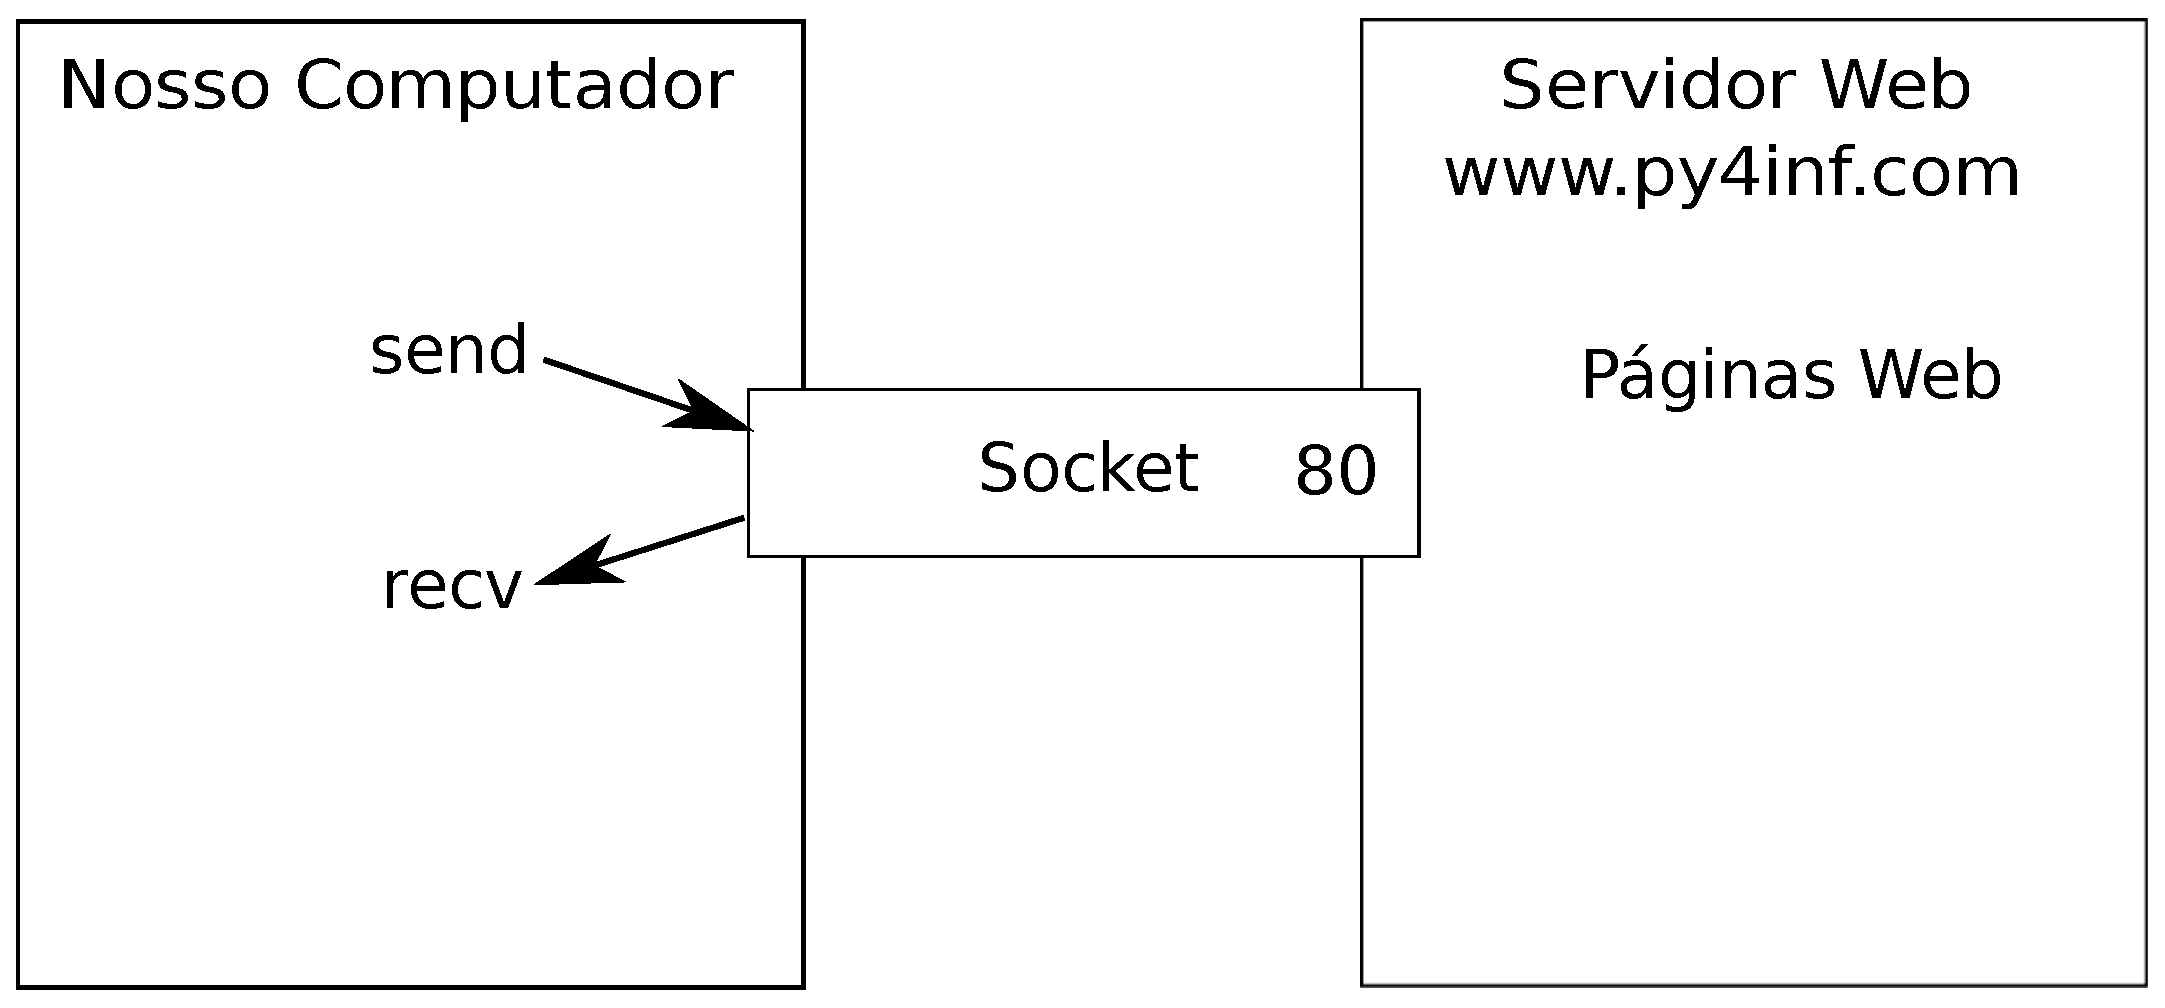
\includegraphics[height=1.50in]{figs2/socket.eps}}
\afterfig

Uma vez enviada a linha em branco, nós escrevemos um loop que recebe do
socket dados em pedaços de 512 caracteres e imprime os dados até que não
exista mais dados para ler (por exemplo, a recv() retorna uma string vazia).

O programa produz a seguinte saída:

\beforeverb
\begin{verbatim}
HTTP/1.1 200 OK
Date: Sun, 14 Mar 2010 23:52:41 GMT
Server: Apache
Last-Modified: Tue, 29 Dec 2009 01:31:22 GMT
ETag: "143c1b33-a7-4b395bea"
Accept-Ranges: bytes
Content-Length: 167
Connection: close
Content-Type: text/plain

But soft what light through yonder window breaks
It is the east and Juliet is the sun
Arise fair sun and kill the envious moon
Who is already sick and pale with grief
\end{verbatim}
\afterverb
%
A saída começa com os cabeçalhos que o servidor web envia
para descrever o documento.
Por exemplo, o cabeçalho {\tt Content-Type} indica que
o documento é um documento em texto plano ({\tt text/plain}).

Depois que o servidor nos enviar os cabeçalhos, ele adiciona uma
linha em branco para indicar o final dos cabeçalhos, e então, envia
realmente os dados do arquivo {\tt romeo.txt}.

Esse exemplo mostra como fazer uma conexão de rede de baixo nível
com sockets.   Sockets podem ser usados para se comunicar com um
servidor web ou com um servidor de email ou muitos outros tipos
de servidores. Tudo que é preciso é encontrar o documento que
descreve o protocolo e escrever o código para enviar e receber os 
dados de acordo com o protocolo.

Contudo, como o protocolo que nós mais comumente usamos é
o protocolo web HTTP, o Python tem uma biblioteca especificamente
desenvolvida para ter suporte ao protocolo HTTP. E assim, obter 
documentos e dados através da web.

\section{Obtendo uma imagem através do HTTP}

\index{urllib!image}
\index{image!jpg}
\index{jpg}
No exemplo acima, nós pegamos um arquivo em texto plano 
que tinha nova linhas dentro do arquivo e nós simplesmente
copiamos os dados para a tela a medida que o programa era
executado.   Nós podemos usar um programa similar para
obter uma imagem através da web usando o HTTP.   Ao invés de
copiar os dados para a tela, a medida que o programa é
executado, nós acumulamos os dados em uma string, retiramos
os cabeçalhos, e então salvamos os dados da imagem em um
arquivo. Como a seguir:

\beforeverb
\begin{verbatim}
import socket
import time

mysock = socket.socket(socket.AF_INET, socket.SOCK_STREAM)
mysock.connect(('www.py4inf.com', 80))
mysock.send('GET http://www.py4inf.com/cover.jpg HTTP/1.0\n\n')


count = 0
picture = "";
while True:
    data = mysock.recv(5120)
    if ( len(data) < 1 ) : break
    # time.sleep(0.25)
    count = count + len(data)
    print len(data),count
    picture = picture + data

mysock.close()

# Look for the end of the header (2 CRLF)
pos = picture.find("\r\n\r\n");
print 'Header length',pos
print picture[:pos]

# Skip past the header and save the picture data
picture = picture[pos+4:]
fhand = open("stuff.jpg","wb")
fhand.write(picture);
fhand.close()
\end{verbatim}
\afterverb
%
Quando o programa é executado, ele produz a seguinte saída:

\beforeverb
\begin{verbatim}
$ python urljpeg.py 
2920 2920
1460 4380
1460 5840
1460 7300
...
1460 62780
1460 64240
2920 67160
1460 68620
1681 70301
Header length 240
HTTP/1.1 200 OK
Date: Sat, 02 Nov 2013 02:15:07 GMT
Server: Apache
Last-Modified: Sat, 02 Nov 2013 02:01:26 GMT
ETag: "19c141-111a9-4ea280f8354b8"
Accept-Ranges: bytes
Content-Length: 70057
Connection: close
Content-Type: image/jpeg
\end{verbatim}
\afterverb
%
Você pode ver que nesse caso, o cabeçalho 
{\tt Content-Type} indica que o corpo do
documento é uma imagem ({\tt image/jpeg}).
Uma vez terminado o programa, você pode ver os dados da imagem
abrindo o arquivo {\tt stuff.jpg} com um visualizador
de imagems.

Durante a execução do programa, você pode ver que nós não temos
5120 caracteres para cada vez que nós chamamos o método
{\tt recv()}. Nós pegamos tantos caracteres quantos foram
transferidos através da rede, do servidor web para nós, no momemto que
nós chamamos {\tt recv()}.  Neste exemplo, nós pegamos 1460 ou 2920 
caracteres cada vez que nós o solicitamos até chegar a 5120 caracteres
de dados.

Os seus resultados podem ser diferentes, dependendo da velocidade de
sua rede.  Note também que na última chamada de {\tt recv()}, nós pegamos
1681 bytes, que é o final do fluxo (stream), e na chamada seguinte da
{\tt recv()} nós recebemos uma string vazia (zero-length). Que nos informa
que o servidor chamou {\tt close()} no seu final de socket e não existe mais
dados para enviar.

\index{time}
\index{time.sleep}
Nós podemos reduzir nossas sucessivas chamada a {\tt recv()}  descomentando
( tirar o '#') a chamada de {\tt time.sleep()}.  Desta forma, nós esperamos
um quarto de segundo depois de cada chamada, e assim, o servidor pode
``se anteceder'' à nós e enviar mais dados antes de nós chamarmos
{\tt recv()} novamente.  Com esse "atraso", o programa é executado
como a seguir:
\beforeverb
\begin{verbatim}
$ python urljpeg.py 
1460 1460
5120 6580
5120 11700
...
5120 62900
5120 68020
2281 70301
Header length 240
HTTP/1.1 200 OK
Date: Sat, 02 Nov 2013 02:22:04 GMT
Server: Apache
Last-Modified: Sat, 02 Nov 2013 02:01:26 GMT
ETag: "19c141-111a9-4ea280f8354b8"
Accept-Ranges: bytes
Content-Length: 70057
Connection: close
Content-Type: image/jpeg
\end{verbatim}
\afterverb
%
Agora, ao invéz de uma primeira e última chamada a {\tt recv()}, nós agora
pegamos 5120 caracteres cada vez que nós pedimos por novos dados.  

Existe um buffer entre o servidor fazendo solicitações {\tt send()} 
e nossa aplicação fazendo solicitações {\tt recv()}.  Quando nós
executamos o programa com o "atraso" estando ativo, em algum momento
o servidor preenche o buffer no socket e é forçado a fazer uma pausa
até que nosso programa comece a esvaziar o buffer.  A pausa, tanto do
envio quanto do recebimento da aplicação, é chamada ``flow control''
(controle de fluxo).
\index{flow control}

\section{Obtendo páginas web com {\tt urllib}}

Embora nós possamos manualmente enviar e receber dados pelo HTTP 
usando a biblioteca socket, existe uma maneira muito mais simples
de realizar essa tarefa comum em Python pelo uso da biblioteca
{\tt urllib}.

Usando a {\tt urllib}, você pode tratar uma página web
de maneira muito parecida a um arquivo.   Você simplesmente
indica qual página web você gostaria de obter e a
{\tt urllib} lida com todo o protocolo HTTP e detalhes sobre
cabeçalhos.

O código equivalente para ler o arquivo {\tt romeo.txt} a partir
da web usando a {\tt urllib} é como o seguinte:

\beforeverb
\begin{verbatim}
import urllib

fhand = urllib.urlopen('http://www.py4inf.com/code/romeo.txt')
for line in fhand:
   print line.strip()
\end{verbatim}
\afterverb
%
Uma vez que a página web tenha sido aberta com 
{\tt urllib.urlopen}, nós podemos tratá-la
como um arquivo e fazer a leitura usando um loop
{\tt for}.   

Quando o programa é executado, nós apenas vemos na
saída o conteúdo do arquvio.   Os cabeçalhos
continuam sendo enviados, mas o código da {\tt urllib}
consome os cabeçalhos e apenas retorna os dados para
nós.

\beforeverb
\begin{verbatim}
But soft what light through yonder window breaks
It is the east and Juliet is the sun
Arise fair sun and kill the envious moon
Who is already sick and pale with grief
\end{verbatim}
\afterverb
%

Como um exemplo, nós podemos escrever 
um programa para obter os dados de
{\tt romeo.txt} e calcular a frequencia
de cada palavra existente dentro do arquivo como a seguir:

\beforeverb
\begin{verbatim}
import urllib

counts = dict()
fhand = urllib.urlopen('http://www.py4inf.com/code/romeo.txt')
for line in fhand:
    words = line.split()
    for word in words:
        counts[word] = counts.get(word,0) + 1   
print counts
\end{verbatim}
\afterverb
%
Novamente, uma vez que nós abrimos a página web, 
nós podemos fazer a leitura como um arquivo local.

\section{Analizando o HTML e varrendo a web}
\index{web!scraping}
\index{parsing HTML}

Um dos usos comuns da capacidade da {\tt urllib} em Python é 
{\bf varrer} a web.   Varrer a web é quando nós escrevemos um programa
que finge ser um navegador web e obtêm páginas, e então examina os dados
nessas páginas a procura de padrões.

Como um exemplo, um mecanismo de busca como o Google irá olhar os fontes
de uma página web e extrair os links para outras páginas e obter
essas páginas, extrair os links para outras páginas e obter essas
páginas, extrair links e assim por diante.   Usando essa técnica,
o Google {\bf mapeia} seu caminho através de quase todas as páginas
na web.   

O Google também usa a frequencia de links das páginas que ele encontra
para uma página em particular de maneira a medir o quão ``importante'' 
uma página é e em que altura a página de aparecer em seus resultados de
pesquisa.

\section{Analisando o HTML através do uso de expressões regulares}

Uma maneira simples de analisar o HTML é usar expressões regulares, para
repetidamente, buscar por e extrair substrings que coincidam com um
padrão em particular.

Aqui está uma página web simples:

\beforeverb
\begin{verbatim}
<h1>The First Page</h1>
<p>
If you like, you can switch to the
<a href="http://www.dr-chuck.com/page2.htm">
Second Page</a>.
</p>
\end{verbatim}
\afterverb
%
Nós podemos construír um expressão regular bem formada para
identificar e extrair os valores dos links do texto abaixo,
como a seguir:

\beforeverb
\begin{verbatim}
href="http://.+?"
\end{verbatim}
\afterverb
%
Nossa expressão regular procura por strings que iniciam com
``href="http://'', seguida de um ou mais caracteres
(``.+?''), seguida por outra aspas.  O ponto de interrogação 
adicionado ao ``.+?'' indica que a expressão é para coincidir
com um padrão de forma ``não gananciosa'', ao invéz de uma
maneira ``gananciosa''. Um padrão não ganancioso tenta encontrar
a {\em menor} string correspondnte possível e a ganaciosa tenta
encontrar a {\em maior} string correspondente possível.
\index{greedy}
\index{non-greedy}

Nós adicionamos parênteses a nossa expressão regular para indicar
qual parte de nossa string correspondente nós gostariamos de extrair, e
foi produzido o seguinte programa:
\index{regex!parentheses}
\index{parentheses!regular expression}

\beforeverb
\begin{verbatim}
import urllib
import re

url = raw_input('Enter - ')
html = urllib.urlopen(url).read()
links = re.findall('href="(http://.*?)"', html)
for link in links:
    print link
\end{verbatim}
\afterverb
%
O mêtodo de expressão regular {\tt findall} irá retornar para nós uma
lista de todas as strings que coincidem com nossa expressão regular,
retornando apenas o texto do link entre as aspas duplas.

Quando nós executamos o programa, nós temos a seguinte saída:

\beforeverb
\begin{verbatim}
python urlregex.py 
Enter - http://www.dr-chuck.com/page1.htm
http://www.dr-chuck.com/page2.htm

python urlregex.py 
Enter - http://www.py4inf.com/book.htm
http://www.greenteapress.com/thinkpython/thinkpython.html
http://allendowney.com/
http://www.py4inf.com/code
http://www.lib.umich.edu/espresso-book-machine
http://www.py4inf.com/py4inf-slides.zip
\end{verbatim}
\afterverb
%
As expressões regulares funcionam muito bem quando o seu HTML está bem
formatado e previsível.  Mas como existem muitas páginas HTML ``quebradas''
por aí, a solução usando expressões regulares pode tanto perder alguns
links válidos qunato terminar com dados ruins.

Isso pode ser resolvido pelo uso de uma robusta biblioteca de análise
de HTML.

\section{Analisando o HTML com o uso da BeautifulSoup}
\index{BeautifulSoup}

Existem várias bibliotecas Python que podem ajudar você a analisar
o HTML e extrair dados das páginas.  Cada uma das bibliotecas
tem suas vantagens e desvantagens e você pode escolher uma com base
em suas necessidades.

Como um exemplo, nós iremos simmplesmente analisar alguma entrada HTML 
e extrair os links usando a biblioteca {\bf BeautifulSoup}.   
Você pode baixar e instalar o código BeautifulSoup de:

\url{http://www.crummy.com/software/}

Você pode baixar e fazer o ``install'' de BeautifulSoup ou você 
pode simplesmente colocar o arquivo {\tt BeautifulSoup.py} no mesmo
diretório que está sua aplicação.

Ainda que o HTML pareça com XML\footnote{O formato XML format é
descrito no próximo capítulo.} e algumas páginas são cuidadosamente 
construidas para ser um XML, a maioria do HTML é, geralmente, quebrado.
O que faz com que um analisador XML rejeite toda a página HTML por
concluir que ela está impropriamente formada.  A BeautifulSoup tolera
muitas imperfeições HTML e ainda consegue que você extraia facilmente
os dados que você precisa.

Nós iremos usar a {\tt urllib} para ler a página e então usar a
{\tt BeautifulSoup} para extrair os atributos {\tt href} das tags
de ancoragem ({\tt a}).
\index{BeautifulSoup}
\index{HTML}
\index{parsing!HTML}

\beforeverb
\begin{verbatim}
import urllib
from BeautifulSoup import *

url = raw_input('Enter - ')
html = urllib.urlopen(url).read()
soup = BeautifulSoup(html)

# Retrieve all of the anchor tags
tags = soup('a')
for tag in tags:
   print tag.get('href', None)
\end{verbatim}
\afterverb
%
O programa pede um endereço web, e então abre a página web,
lê os dados e passa os dados para o analizador BeautifulSoup, 
e então obtêm todas as tags de ancoragem e imprime o atributo
{\tt href} de cada tag.

Quando o programa é executado, ele se parece como a seguir:

\beforeverb
\begin{verbatim}
python urllinks.py 
Enter - http://www.dr-chuck.com/page1.htm
http://www.dr-chuck.com/page2.htm

python urllinks.py 
Enter - http://www.py4inf.com/book.htm
http://www.greenteapress.com/thinkpython/thinkpython.html
http://allendowney.com/
http://www.si502.com/
http://www.lib.umich.edu/espresso-book-machine
http://www.py4inf.com/code
http://www.pythonlearn.com/
\end{verbatim}
\afterverb
%
Você pode usar a BeautifulSoup para buscar várias partes de cada 
tag como a seguir:

\beforeverb
\begin{verbatim}
import urllib
from BeautifulSoup import *

url = raw_input('Enter - ')
html = urllib.urlopen(url).read()
soup = BeautifulSoup(html)

# Retrieve all of the anchor tags
tags = soup('a')
for tag in tags:
   # Look at the parts of a tag
   print 'TAG:',tag
   print 'URL:',tag.get('href', None)
   print 'Content:',tag.contents[0]
   print 'Attrs:',tag.attrs
\end{verbatim}
\afterverb
%
Isso produz a seguinte saída:

\beforeverb
\begin{verbatim}
python urllink2.py 
Enter - http://www.dr-chuck.com/page1.htm
TAG: <a href="http://www.dr-chuck.com/page2.htm">
Second Page</a>
URL: http://www.dr-chuck.com/page2.htm
Content: [u'\nSecond Page']
Attrs: [(u'href', u'http://www.dr-chuck.com/page2.htm')]
\end{verbatim}
\afterverb
%
Esses exemplos apenas começam a mostrar o poder da BeautifulSoup,
quando se refere a análise de HTML.  Veja a documentação e exemplos
em
\url{http://www.crummy.com/software/BeautifulSoup/} para mais detalhes.

\section{Lendo arquivos binários usando a urllib}

Algumas vezes, você quer obter um arquivo não texto (ou binário), como
um arquivo de imagem ou vídeo. Os dados nesses arquivos geralmente não
são úteis para serem impressos, mas você pode facilmente fazer uma cópia
da URL para um arquivo local em seu disco rígido usando a {\tt urllib}.
\index{binary file}

O padrão é abrir a URL e usar {\tt read} para baixar o conteúdo completo
do documento para dentro de uma variável string ({\tt img}), e então
escrever essa informação em um arquivo local, como a seguir:

\beforeverb
\begin{verbatim}
img = urllib.urlopen('http://www.py4inf.com/cover.jpg').read()
fhand = open('cover.jpg', 'w')
fhand.write(img)
fhand.close()
\end{verbatim}
\afterverb
%
Esse programa lê todos os dados, de uma vez, através da rede e 
os armazena dentro da variável {\tt img}, na principal memória de seu,
computaor. Então abre o arquivo {\tt cover.jpg} e escreve os dados para
o seu disco.  Isso irá funcionar se o tamanho do arquivo for menor que
o tamanho da memória de seu computador.

Contudo, se ele for um arquivo de áudio ou vídeo grande, esse programa
pode falhar ou pelo memos rodar de forma extremamente vagarosa quando seu
computador ficar sem memória.  Para evitar ficar sem memória, nós podemos
obter os dados em blocos (ou buffers) e então escrever cada bloco no disco
antes de obter o próximo bloco.  Desta forma o programa pode ler um arquivo
de qualquer tamanho sem usar toda a memória que você tem em seu computador.

\beforeverb
\begin{verbatim}
import urllib

img = urllib.urlopen('http://www.py4inf.com/cover.jpg')
fhand = open('cover.jpg', 'w')
size = 0
while True:
    info = img.read(100000)
    if len(info) < 1 : break
    size = size + len(info)
    fhand.write(info)

print size,'characters copied.'
fhand.close()
\end{verbatim}
\afterverb
%
Neste exemplo, nós lemos apenas 100,000 caracteres por vez e então 
escrevemos esses caracteres no arquivo {\tt cover.jpg} antes de obter
os próximos 100,000 caracteres de dados a partir da web.

Esse programa é executado como a seguir:

\beforeverb
\begin{verbatim}
python curl2.py 
568248 characters copied.
\end{verbatim}
\afterverb
%

Se você tem um computador Unix ou Macintosh, você provavelmente tem um
comando em seu sistema operacional que executa essa operação,
como a seguir:
\index{curl}

\beforeverb
\begin{verbatim}
curl -O http://www.py4inf.com/cover.jpg
\end{verbatim}
\afterverb
%
O comando {\tt curl} é a abreviação para ``copy URL'', então esses dois 
exemplos são, inteligentemente, chamados de {\tt curl1.py} e {\tt curl2.py} em 
\url{www.py4inf.com/code}, já que eles implementam uma funcionalidade similar
ao comando {\tt curl}.  Existe também um programa exemplo {\tt curl3.py} que
realiza essa tarefa de maneira um pouco mais efetiva, no caso de você
realmente quiser usar esse padrão em um programa que você estiver escrevendo.

\section{Glolossário}

\begin{description}

\item[BeautifulSoup:] Uma biblioteca Python para análise de documentos HTML
e extração de dados desses documentos HTML que faz compensações nas
maiorias das imperfeições em um HTML que os navegadores geralmente ignoram.
Você pode baixar o código da BeautifulSoup em 
\url{www.crummy.com}.
\index{BeautifulSoup}

\item[port:] Um número que geralmente indica qual aplicação 
você está contactando quando você faz uma conexão por socket com um servidor.
Como um exemplo, o tráfego web, usualmente, usa a porta 80, enquanto o
tráfego de email usa a porta 25.
\index{port}

\item[scrape:] Quando um programa finge ser um navegador web,
obtêm uma página web, e então olha o conteúdo da página web. 
Geralmente os programas estão seguindo os links de uma página para
encontrar a próxima página. Para que eles possam atravessar uma rede de páginas
ou uma rede social.
\index{socket}

\item[socket:] Uma conexão de rede entre duas aplicações. Onde as
aplicações podem enviar e receber dados em ambas as direções.
\index{socket}

\item[spider:] O ato de um mecanismo de busca pela web obtendo uma
página e então todas as páginas com ligações a partir dessa página e
assim por diante até ele ter praticamente todas as páginas na Internet que
ele usará para construir sua indexação de busca.
\index{spider}

\end{description}

\section{Exercícios}

\begin{ex}
Altere o programa socket {\tt socket1.py} para pedir ao usuário a 
URL, e assim, ele possa ler qualquer página web.  
Você pode usar {\tt split('/')} para quebrar a URL em partes de componentes
para que você possa extrair o nome da máquina para a chamada {\tt connect}.
Adicionar uma checagem de erro usando {\tt try} e {\tt except} para lidar
com a conexão, caso o usuário digite um formato de URL impróprio ou
não existente.  
\end{ex}

\begin{ex}
Altere seu programa socket para que ele conte o número de caracteres que ele
tenha recebido e interrompa a exibição de qualquer texto após ele ter mostrado
3000 caracteres.  O programa deve obter o documento por inteiroi, contar o
número total de caracteres e exibir a contagem do número de caracteres no
final do documento.
\end{ex}

\begin{ex}
Use a {\tt urllib} para replicar o exercíco prévio de (1) obtenção de um
documento a partir de uma URL, (2) exibindo até 3000 caracteres, e (3) 
desfazendo a contagem do total de caracteres no documento.  Não se preocupe
com os cabeçalhos neste exercíco, apenas mostre os primeiros 3000 caracteres
do conteúdo do documento.
\end{ex}

\begin{ex}
Altere o programa {\tt urllinks.py} para que ele extraia e conte 
as tags parágrafo (p) de um documento HTML obtido e exiba a contagem
de parágrafos como saída de seu programa.  
Não exiba o texto de parágrafo, apenas faça a contagem.
Teste seu programa em várias páginas web pequenas. E também em algumas
páginas web grandes.
\end{ex}

\begin{ex}
(Avançado) Altere o programa socket para que ele apenas mostre os dados
após os cabeçalhos e uma linha em branco tiverem sido recebidos.  Lembre 
que o {\tt recv} está recebendo caracteres (nova linha e outros mais),
não linhas.
\end{ex}



% TODO % The contents of this file is 
% Copyright (c) 2009-  Charles R. Severance, All Righs Reserved

\chapter{Usando Web Services}
%\chapter{Using Web Services}

Agora que se tornou mais facil retornar e analizar documentos
HTTP utilizando programas, não levará muito tempo para desenvolver
um sistema onde nós podemos começar à produzir documentos que serão
especificamente desenhados para serem utilizados por outros
programas (i.e., nenhum HTML para ser mostrado no navegador)
%Once it became easy to retrieve documents and parse documents 
%over HTTP using programs, it did not take long to develop 
%an approach where we started producing documents that were specifically
%designed to be consumed by other 
%programs (i.e., not HTML to be displayed in a browser).

Existem dois formatos comuns que nós usamos quando trocamos dados através da web.
O ``eXtensible Markup Language'' ou XML é utilizado à muito tempo
e é melhor desenhado para troca de document-style-data. Quando programas somente
querem trocar dicionarios, listas, ou outra informaçao interterna entre eles, 
eles usam JavaScript Object Notation ou JSON (sobre \url{www.json.org}).
Nós vamos ver os dois formatos.
%There are two common formats that we use when exchanging data across the web.
%The ``eXtensible Markup Language'' or XML has been in use for a very long time 
%and is best suited for exchanging document-style data.   When programs just want 
%to exchange dictionaries, lists, or other internal information with each other,
%they use JavaScript Object Notation or JSON (see \url{www.json.org}).  
%We will look at both formats.

\section{eXtensible Markup Language - XML}
%\section{eXtensible Markup Language - XML}

O XML é bem parecido com o HTML, porem o XML é melhor estruturado
que o HTML. Aqui está um exemplo de um documento XML:
%XML looks very similar to HTML, but XML is more structured 
%than HTML.  Here is a sample of an XML document:

\beforeverb
\begin{verbatim}
<person>
  <name>Chuck</name>
  <phone type="intl">
     +1 734 303 4456
   </phone>
   <email hide="yes"/>
</person>
\end{verbatim}
\afterverb
%
É mais facil pensar em um documento XML como uma estrutura em arvore
onde tem uma tag no topo {\tt person} e outras tags como {\tt phone}
são escritas como \emph{filhos} dos pais deles. 
%Often it is helpful to think of an XML document as a tree structure
%where there is a top tag {\tt person} and other tags such as {\tt phone}
%are drawn as \emph{children} of their parent nodes.

\beforefig
\centerline{\includegraphics[height=1.50in]{figs2/xml-tree.eps}}
\afterfig

\section{Analizando o XML}
%\section{Parsing XML}

\index{ElementTree}
\index{ElementTree!fromstring}
\index{ElementTree!find}

Aqui está uma simples aplicação que analiza algum XML
e extrai alguns elementos do XML:
%Here is a simple application that parses some XML
%and extracts some data elements from the XML:

\beforeverb
\begin{verbatim}
import xml.etree.ElementTree as ET

data = '''
<person>
  <name>Chuck</name>
  <phone type="intl">
     +1 734 303 4456
   </phone>
   <email hide="yes"/>
</person>'''

tree = ET.fromstring(data)
print 'Name:',tree.find('name').text
print 'Attr:',tree.find('email').get('hide')
\end{verbatim}
\afterverb
%
Ao chamar {\tt fromstring} é feita a conversão da string que 
representa o XML em uma ``arvore'' de conecções XML. Quando o
XML esta em uma arvore, nós temos uma serie de metodos que nós
podemos chamar para exrair informações do XML.
%Calling {\tt fromstring} converts the string representation
%of the XML into a ``tree'' of XML nodes.  When the
%XML is in a tree, we have a series of methods we can call to 
%extract portions of data from the XML.  

A função {\tt find} varre a arvore do XML
e retorna um {\bf nó} que corresponde à aquela tag especifica.
Cada nó pode conter algum texto, alguns atributos (como hide), e
algum nó ``filho''. Cada nó pode ser o inicio de uma arvore de nós.
%The {\tt find} function searches through the 
%XML tree and retrieves a {\bf node} that matches the specified tag.
%Each node can have some text, some attributes (like hide), and
%some ``child'' nodes.   Each node can be the top of a tree of nodes.

\beforeverb
\begin{verbatim}
Name: Chuck
Attr: yes
\end{verbatim}
\afterverb
%
Utilizar um analizador de XML como o {\tt ElementTree} teremos a
vantagem que, enquanto o XML deste exemplo é bastante simples, 
teremos muitas regras em relação à XML validos e usar o 
{\tt ElementTree} nos permitirá extrair informações do XML sem
se preoculpar com as regras de sintaxe do XML.
%Using an XML parser such as {\tt ElementTree} has the advantage
%that while the XML in this example is quite simple, it turns
%out there are many rules regarding valid XML and using 
%{\tt ElementTree} allows us to extract data from XML without 
%worrying about the rules of XML syntax.

\section{Percorrendo os nós}
%\section{Looping through nodes}

\index{ElementTree!findall}
\index{ElementTree!get}
Frequentemente o XML terá multiplos nós que nós podemos percorrer
para processar todos os nós. No programa a seguir,
nós percorremos por todos os nós do {\tt user}:
%Often the XML has multiple nodes and we need to write a loop
%to process all of the nodes.  In the following program, 
%we loop through all of the {\tt user} nodes:

\beforeverb
\begin{verbatim}
import xml.etree.ElementTree as ET

input = '''
<stuff>
    <users>
        <user x="2">
            <id>001</id>
            <name>Chuck</name>
        </user>
        <user x="7">
            <id>009</id>
            <name>Brent</name>
        </user>
    </users>
</stuff>'''

stuff = ET.fromstring(input)
lst = stuff.findall('users/user')
print 'User count:', len(lst)

for item in lst:
    print 'Name', item.find('name').text
    print 'Id', item.find('id').text
    print 'Attribute', item.get('x')
\end{verbatim}
\afterverb
%
O metodo {\tt findall} retorna uma lista do Python com sub-árvores
que representam a estrutura {\tt user} da árvore do XML. Então nós 
podemos escrever um loop {\tt for} que procura em cada nó do user,
e imprime os elementos {\tt name} e {\tt id} assim como o 
atributo {\tt x} do nó {\tt user}.
%The {\tt findall} method retrieves a Python list of subtrees that
%represent the {\tt user} structures in the XML tree.  Then we can 
%write a {\tt for} loop that looks at each of the user nodes, and 
%prints the {\tt name} and {\tt id} text elements as well as the 
%{\tt x} attribute from the {\tt user} node.

\beforeverb
\begin{verbatim}
User count: 2
Name Chuck
Id 001
Attribute 2
Name Brent
Id 009
Attribute 7
\end{verbatim}
\afterverb
%

\section{JavaScript Object Notation - JSON}
%\section{JavaScript Object Notation - JSON}
\index{JSON}
\index{JavaScript Object Notation}

O formato JSON foi inspirado no formato do objeto array utilizado na linguagem JavaScript.
Mas como o Python foi inventado antes do JavaScript, a sintaxe que o Python utiliza
para dicionarios e listas influenciaram na sintaxe do JSON. Então o formato JSON é
bem parecido com a combinação de listas e dicionarios do Python.
%The JSON format was inspired by the object and array format used in the JavaScript
%language.  But since Python was invented before JavaScript, Python's syntax
%for dictionaries and lists influenced the syntax of JSON.  So the format of JSON
%is nearly identical to a combination of Python lists and dictionaries.

Aqui está uma codificação JSON que é quase equivalente ao simples XML abaixo:
%Here is a JSON encoding that is roughly equivalent to the simple XML from above:

\beforeverb
\begin{verbatim}
{
  "name" : "Chuck",
  "phone" : {
    "type" : "intl",
    "number" : "+1 734 303 4456"
   },
   "email" : {
     "hide" : "yes"
   }
}
\end{verbatim}
\afterverb
%
Você pode notar algumas diferenças. Primeira, no XML, nós podemos adicionar
atributos como ``intl'' à tag ``phone''. No JSON, nós simplesmente temos chaves de
valores pares. Além de que a tag ``person'' não existe mais, que substituida por
um conjunto de chaves externas.
%You will notice some differences.  First, in XML, we can add attributes like
%``intl'' to the ``phone'' tag.  In JSON, we simply have key-value pairs.  Also
%the XML ``person'' tag is gone, replaced by a set of outer curly braces.  

No geral, a estrutura JSON é mais simples que a do XML por conta do JSON ter menos
utilidades que o XML. Mas o JSON tem a vantagem de mapear {\em directly} para alguma
combinação de dicionarios e listas. E como quase todas as linguagens de programação 
tem algo equivalente aos dicionarios e listas do Python, JSON é um formato natural 
para fazer dois programas cooperarem e trocarem dados.
%In general, JSON structures are simpler than XML because JSON has fewer capabilities
%than XML.  But JSON has the advantage that it maps {\em directly} to some combination
%of dictionaries and lists.   And since nearly all programming languages 
%have something equivalent to Python's dictionaries and lists, JSON is a very
%natural format to have two cooperating programs exchange data.

JSON está facilmente se tornando o formato escolhido para realizar troca de dados
entre aplicações por conta de sua simplicidade se comparado ao XML.
%JSON is quickly becoming the format of choice for nearly all data exchange between 
%applications because of its relative simplicity compared to XML.

\section{Analizando JSON}
%\section{Parsing JSON}

Nós podemos contruir nosso JSON utilizando dicionarios (objetos) e listas conforme
o necessario. Neste exemplo, n´os vamos representar uma lista de usuarios onde cada
usuario é um valor de chave (i.e., um dicionario). Então nós temos uma lista de
dicionarios.
%We construct our JSON by nesting dictionaries (objects) and lists as needed.  In 
%this example, we represent a list of users where each user is a set of 
%key-value pairs (i.e., a dictionary).  So we have a list of dictionaries.

No programa a seguir, nós usamos o biblioteca contrutora {\bf json} para analizar
o JSON e ler as informações. Compare ele de perto com a informação equivalente em XML
abaixo. O JSON tem menos detalhes, então nós devemos previamente saber que nós
estamos pegando uma lista e essa lista são usuarios e cada usuario é uma valor de 
chave. O JSON é mais sucinto (uma vantagem) mas também é menos auto-explicativo 
(uma desvantagem).
%In the following program, we use the built-in {\bf json} library to parse 
%the JSON and read through the data.   Compare this closely to the equivalent
%XML data and code above.  The JSON has less detail, so we must know in advance 
%that we are getting a list and that the list is of users and each user is a
%set of key-value pairs.  The JSON is more succinct (an advantage) but also is 
%less self-describing (a disadvantage).

\beforeverb
\begin{verbatim}
import json

input = '''
[
  { "id" : "001",
    "x" : "2",
    "name" : "Chuck"
  } ,
  { "id" : "009",
    "x" : "7",
    "name" : "Brent"
  } 
]'''

info = json.loads(input)
print 'User count:', len(info)

for item in info:
    print 'Name', item['name']
    print 'Id', item['id']
    print 'Attribute', item['x']
\end{verbatim}
\afterverb
%

Se você comparar o codigo para extrarir a informação do JSON e XML analizados,
você vera que oque nós pegamos do {\bf json.loads()} é uma lista Python
que nós percorremos com um {\tt for} loop, e cada item dentro desta lista
é um dicionario Python. Uma vez que o JSON foi analizado, nós podemos usar o
operador de indice do Python para extrair varias informações de cada usuario.
Nós não precisamos usar a biblioteca JSON para percorrer o JSON analizado, 
pois ela retornará uma informação já é uma estrutura do proprio Python.
%If you compare the code to extract data from the parsed JSON and XML
%you will see that what we get from {\bf json.loads()} is a Python list
%which we traverse with a {\tt for} loop, and each item within that list
%is a Python dictionary.  Once the JSON has been parsed, we can use the Python
%index operator to extract the various bits of data for each user.  We don't
%have to use the JSON library to dig through the parsed JSON, since the returned
%data is simply native Python structures.

A saida deste programa é exatamente a mesma que a versão em XML abaixo.
%The output of this program is exactly the same as the XML version above.

\beforeverb
\begin{verbatim}
User count: 2
Name Chuck
Id 001
Attribute 2
Name Brent
Id 009
Attribute 7
\end{verbatim}
\afterverb
%
Em geral, existem uma tendencia da industria utilizar cada vez mais o JSON
do que o XML em serviços web. Por conta do JSON ser mais simples e mais
direcionado para estruturas nativas que já existem nas linguagens de
programação, a analize e extração de dados é usualmente simples e mais direto
utilizando JSON. Mas o XML é mais auto-explicativo que o JSON então terá
algumas aplicações em que o XML detem a vantagem. Por exemplo, a maioria de 
processadores de palavras guardam documentos internamente utilizando XML
em vez de JSON.
%In general, there is an industry trend away from XML and towards JSON for 
%web services.  Because the JSON is simpler and more directly maps to native 
%data structures we already have in programming languages, the parsing 
%and data extraction code is usually simpler and more direct when using JSON.
%But XML is more self-descriptive than JSON and so there are 
%some applications where XML retains an advantage.  For example, most word 
%processors store documents internally using XML rather than JSON.

\section{Application Programming Interfaces}

We now have the ability to exchange data between applications using HyperText
Transport Protocol (HTTP) and a way to represent complex data that we are 
sending back and forth between these applications using eXtensible 
Markup Language (XML) or JavaScript Object Notation (JSON).

The next step is to begin to define and document ``contracts'' between 
applications using these techniques. The general name for these 
application-to-application contracts is {\bf Application Program 
Interfaces} or APIs.  When we use an API, generally one program
makes a set of {\bf services} available for use by other applications
and publishes the APIs (i.e., the ``rules'') that must be followed to 
access the services provided by the program.

When we begin to build our programs where the functionality of
our program includes access to services provided by other programs, 
we call the approach a {\bf Service-Oriented Architecture} or SOA.
A SOA approach is one where our overall application makes use of 
the services of other applications.  A non-SOA approach is where the
application is a single standalone application which contains all of the
code necessary to implement the application.

We see many examples of SOA when we use the web.  We can go to a single 
web site and book air travel, hotels, and automobiles all from a 
single site.  The data for hotels is not stored on the airline computers. 
Instead, the airline computers contact the services on the hotel computers
and retrieve the hotel data and present it to the user.  When the user
agrees to make a hotel reservation using the airline site, the airline site uses
another web service on the hotel systems to actually make the reservation.
And when it comes time to charge your credit card for the whole transaction, 
still other computers become involved in the process.

\beforefig
\centerline{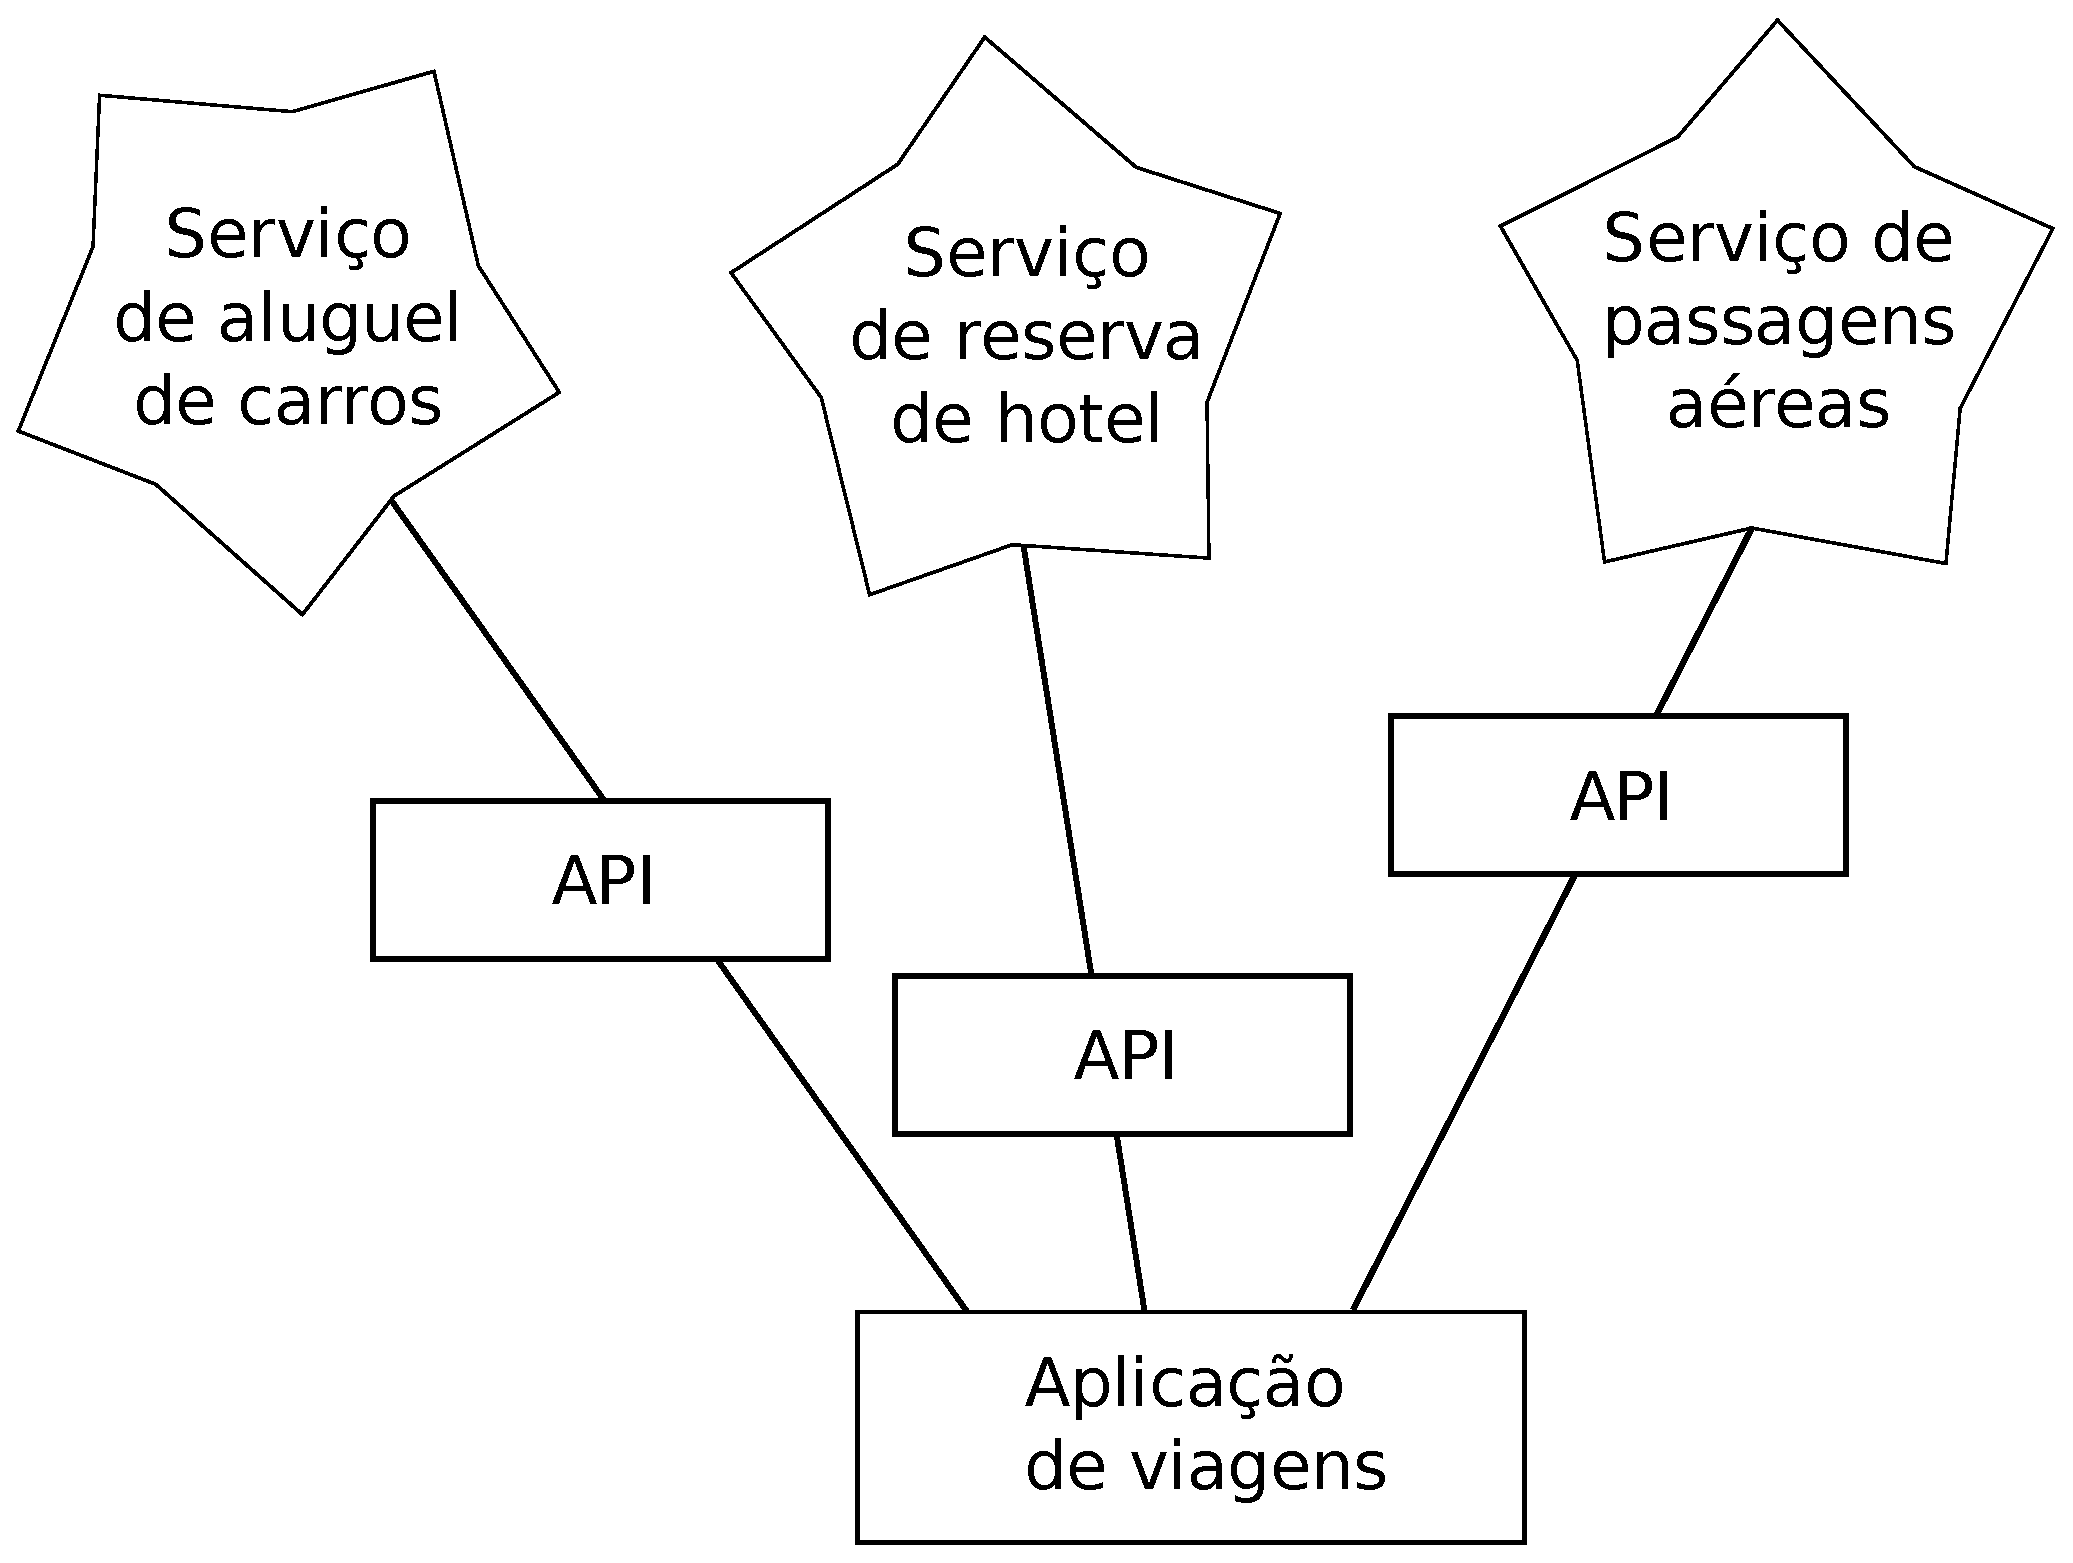
\includegraphics[height=2.50in]{figs2/soa.eps}}
\afterfig

A Service-Oriented Architecture has many advantages including: (1) we 
always maintain only one copy of data (this is particularly important
for things like hotel reservations where we do not want to over-commit)
and (2) the owners of the data can set the rules about the use of their 
data.   With these advantages, an SOA system must be carefully designed
to have good performance and meet the user's needs.

When an application makes a set of services in its API available over the web, 
we call these {\bf web services}. 

\section{Google geocoding web service}
\index{Google}
\index{geocoding}
\index{web service}

Google has an excellent web service that allows us to make use of their 
large database of geographic information.   We can submit a geographical
search string like ``Ann Arbor, MI'' to their geocoding API and have Google 
return its best guess as to where on a map we might find our search string and
tell us about the landmarks nearby.

The geocoding service is free but rate limited so you cannot make unlimited
use of the API in a commercial application.   But if you have some survey data
where an end user has entered a location in a free-format input box, you can use
this API to clean up your data quite nicely.  

{\em When you are using a free API like Google's geocoding API, you need
to be respectful in your use of these resources.  If too many people abuse the
service, Google might drop or significantly curtail its free service.}
\index{rate limiting}

You can read the online documentation for this service, but it is quite simple
and you can even test it using a browser by typing the following URL into your 
browser:

\url{http://maps.googleapis.com/maps/api/geocode/json?sensor=false &address=Ann+Arbor%2C+MI}

Make sure to unwrap the URL and remove any spaces from the URL before pasting
it into your browser.

The following is a simple application to prompt the user for a search string,
call the Google geocoding API, and extract information from the returned JSON.

\beforeverb
\begin{verbatim}
import urllib
import json

serviceurl = 'http://maps.googleapis.com/maps/api/geocode/json?'

while True:
    address = raw_input('Enter location: ')
    if len(address) < 1 : break

    url = serviceurl + urllib.urlencode({'sensor':'false', 
          'address': address})
    print 'Retrieving', url
    uh = urllib.urlopen(url)
    data = uh.read()
    print 'Retrieved',len(data),'characters'

    try: js = json.loads(str(data))
    except: js = None
    if 'status' not in js or js['status'] != 'OK':
        print '==== Failure To Retrieve ===='
        print data
        continue

    print json.dumps(js, indent=4)

    lat = js["results"][0]["geometry"]["location"]["lat"]
    lng = js["results"][0]["geometry"]["location"]["lng"]
    print 'lat',lat,'lng',lng
    location = js['results'][0]['formatted_address']
    print location
\end{verbatim}
\afterverb
%
The program takes the search string and constructs a URL with the
search string as a properly encoded parameter and then uses
{\bf urllib} to retrieve the text from the Google geocoding API.
Unlike a fixed web page, the data we get depends on the parameters
we send and the geographical data stored in Google's servers.

Once we retrieve the JSON data, we parse it with the {\bf json}
library and do a few checks to make sure that we received good data, 
then extract the information that we are looking for.

The output of the program is as follows (some of the returned
JSON has been removed):

\beforeverb
\begin{verbatim}
$ python geojson.py
Enter location: Ann Arbor, MI
Retrieving http://maps.googleapis.com/maps/api/
  geocode/json?sensor=false&address=Ann+Arbor%2C+MI
Retrieved 1669 characters
{
    "status": "OK", 
    "results": [
        {
            "geometry": {
                "location_type": "APPROXIMATE", 
                "location": {
                    "lat": 42.2808256, 
                    "lng": -83.7430378
                }
            }, 
            "address_components": [
                {
                    "long_name": "Ann Arbor", 
                    "types": [
                        "locality", 
                        "political"
                    ], 
                    "short_name": "Ann Arbor"
                } 
            ], 
            "formatted_address": "Ann Arbor, MI, USA", 
            "types": [
                "locality", 
                "political"
            ]
        }
    ]
}
lat 42.2808256 lng -83.7430378
Ann Arbor, MI, USA
Enter location:
\end{verbatim}
\afterverb
%
You can download 
\url{www.py4inf.com/code/geojson.py} and 
\url{www.py4inf.com/code/geoxml.py} to explore the JSON
and XML variants of the Google geocoding API. 

\section{Security and API usage}
\index{OAuth}
\index{API!key}

It is quite common that you need some kind of 
``API key'' to make use of a vendor's API.  The
general idea is that they want to know who is using 
their services and how much each user is using.  
Perhaps they have free and pay tiers of their services
or have a policy that limits the number of requests 
that a single individual can make during a particular 
time period.

Sometimes once you get your API key, you simply include
the key as part of POST data or perhaps as a parameter
on the URL when calling the API.

Other times, the vendor wants increased assurance of
the source of the requests and so they add expect you 
to send cryptographically signed messages using shared
keys and secrets.   A very common technology that is used 
to sign requests over the Internet is called {\bf OAuth}.
You can read more about the OAuth protocol at
\url{http://www.oauth.net}.

As the Twitter API became increasingly valuable, Twitter
went from an open and public API to an API that required
the use of OAuth signatures on each API request. Thankfully
there are still a number of convenient and free OAuth libraries
so you can avoid writing an OAuth implementation from scratch
by reading the specification.  These libraries are of 
varying complexity and have varying degrees of
richness.  The OAuth web site has information about various 
OAuth libraries.

For this next sample program we will download the files 
{\bf twurl.py}, {\bf hidden.py}, 
{\bf oauth.py}, 
and
{\bf twitter1.py} from 
\url{www.py4inf.com/code} and put them all in a folder
on your computer.

To make use of these programs you will need to have a Twitter
account, and authorize your Python code as an application,
set up a key, secret, token and token secret.  You will edit
the file {\bf hidden.py} and put these four strings into the
appropriate variables in the file:

\beforeverb
\begin{verbatim}
    def auth() :
        return { "consumer_key" : "h7L...GNg",
            "consumer_secret" : "dNK...7Q",
            "token_key" : "101...GI",
            "token_secret" : "H0yM...Bo" }
\end{verbatim}
\afterverb
%
The Twitter web service are accessed using a URL like this:

\url{https://api.twitter.com/1.1/statuses/user_timeline.json}

But once all of the security information has been added, the URL
will look more like:

\beforeverb
\begin{verbatim}
https://api.twitter.com/1.1/statuses/user_timeline.json?count=2
&oauth_version=1.0&oauth_token=101...SGI&screen_name=drchuck
&oauth_nonce=09239679&oauth_timestamp=1380395644
&oauth_signature=rLK...BoD&oauth_consumer_key=h7Lu...GNg
&oauth_signature_method=HMAC-SHA1
\end{verbatim}
\afterverb
%
You can read the OAuth specification if you want to
know more about the meaning of the various parameters that
are added to meet the security requirements of OAuth.  

For the programs we run with Twitter, we hide all the 
complexity in the files {\bf oauth.py} and {\bf twurl.py}.
We simply set the secrets in {\bf hidden.py} and then 
send the desired URL to the {\bf twurl.augment()} 
function and the library code adds all the necessary 
parameters to the URL for us.

This program ({\bf twitter1.py}) retrieves the timeline
for a particular Twitter user and returns it to us in JSON
format in a string.  We simply print the first 250 characters
of the string:

\beforeverb
\begin{verbatim}
import urllib
import twurl

TWITTER_URL='https://api.twitter.com/1.1/statuses/user_timeline.json'

while True:
    print ''
    acct = raw_input('Enter Twitter Account:')
    if ( len(acct) < 1 ) : break
    url = twurl.augment(TWITTER_URL,
        {'screen_name': acct, 'count': '2'} )
    print 'Retrieving', url
    connection = urllib.urlopen(url)
    data = connection.read()
    print data[:250]
    headers = connection.info().dict
    # print headers
    print 'Remaining', headers['x-rate-limit-remaining']
\end{verbatim}
\afterverb
%
When the program runs it produces the following output: 
 
\beforeverb
\begin{verbatim}
Enter Twitter Account:drchuck
Retrieving https://api.twitter.com/1.1/ ...
[{"created_at":"Sat Sep 28 17:30:25 +0000 2013","
id":384007200990982144,"id_str":"384007200990982144",
"text":"RT @fixpert: See how the Dutch handle traffic 
intersections: http:\/\/t.co\/tIiVWtEhj4\n#brilliant",
"source":"web","truncated":false,"in_rep
Remaining 178

Enter Twitter Account:fixpert
Retrieving https://api.twitter.com/1.1/ ...
[{"created_at":"Sat Sep 28 18:03:56 +0000 2013",
"id":384015634108919808,"id_str":"384015634108919808",
"text":"3 months after my freak bocce ball accident, 
my wedding ring fits again! :)\n\nhttps:\/\/t.co\/2XmHPx7kgX",
"source":"web","truncated":false,
Remaining 177

Enter Twitter Account:
\end{verbatim}
\afterverb
%
Along with the returned timeline data, Twitter also returns
metadata about the request in the HTTP response headers. 
One header in particular, {\bf x-rate-limit-remaining}, informs
us how many more requests we can make before we will be shut 
off for a short time period.  You can see that our remaining 
retrievals drop by one each time we make a request to the 
API.

In the following example, we retrieve a user's Twitter friends,
parse the returned JSON, and extract some of the information
about the friends.  We also dump the JSON after parsing and
``pretty-print'' it with an indent of four characters to allow
us to pore through the data when we want to extract more fields.

\beforeverb
\begin{verbatim}
import urllib
import twurl
import json

TWITTER_URL = 'https://api.twitter.com/1.1/friends/list.json'

while True:
    print ''
    acct = raw_input('Enter Twitter Account:')
    if ( len(acct) < 1 ) : break
    url = twurl.augment(TWITTER_URL,
        {'screen_name': acct, 'count': '5'} )
    print 'Retrieving', url
    connection = urllib.urlopen(url)
    data = connection.read()
    headers = connection.info().dict
    print 'Remaining', headers['x-rate-limit-remaining']
    js = json.loads(data)
    print json.dumps(js, indent=4)

    for u in js['users'] :
        print u['screen_name']
        s = u['status']['text']
        print '  ',s[:50]
\end{verbatim}
\afterverb
%
Since the JSON becomes a set of nested Python lists and dictionaries,
we can use a combination of the index operation and {\tt for} loops to 
wander through the returned data structures with very little 
Python code.

The output of the program looks as follows (some of the data items 
are shortened to fit on the page):

\beforeverb
\begin{verbatim}
Enter Twitter Account:drchuck
Retrieving https://api.twitter.com/1.1/friends ...
Remaining 14
{
    "next_cursor": 1444171224491980205, 
    "users": [
        {
            "id": 662433, 
            "followers_count": 28725, 
            "status": {
                "text": "@jazzychad I just bought one .__.", 
                "created_at": "Fri Sep 20 08:36:34 +0000 2013", 
                "retweeted": false, 
            }, 
            "location": "San Francisco, California", 
            "screen_name": "leahculver", 
            "name": "Leah Culver", 
        }, 
        {
            "id": 40426722, 
            "followers_count": 2635, 
            "status": {
                "text": "RT @WSJ: Big employers like Google ...", 
                "created_at": "Sat Sep 28 19:36:37 +0000 2013", 
            }, 
            "location": "Victoria Canada", 
            "screen_name": "_valeriei", 
            "name": "Valerie Irvine", 
    ], 
    "next_cursor_str": "1444171224491980205"
}
leahculver
   @jazzychad I just bought one .__.
_valeriei
   RT @WSJ: Big employers like Google, AT&amp;T are h
ericbollens
   RT @lukew: sneak peek: my LONG take on the good &a
halherzog
   Learning Objects is 10. We had a cake with the LO,
scweeker
   @DeviceLabDC love it! Now where so I get that "etc

Enter Twitter Account:
\end{verbatim}
\afterverb
%
The last bit of the output is where we see the for loop reading the
five most recent ``friends'' of the {\bf drchuck} Twitter account 
and printing the most recent status for each friend. There is a 
great deal more data available in the returned JSON.  If you look
in the output of the program, you can also see that the ``find the friends''
of a particular account has a different rate limitation than 
the number of timeline queries we are allowed to run per time period.

These secure API keys allow Twitter to have solid confidence that they 
know who is using their API and data and at what level.   The 
rate-limiting approach allows us to do simple, personal data retrievals but
does not allow us to build a product that pulls data from their API 
millions of times per day.

\section{Glossary}

\begin{description}

\item[API:] Application Program Interface - A contract between
applications that defines the patterns of interaction between 
two application components.
\index{API}

\item[ElementTree:] A built-in Python library used to parse XML data.
\index{ElementTree}

\item[JSON:] JavaScript Object Notation. A format that allows for 
the markup of structured data based on the syntax of JavaScript
Objects.
\index{JSON}
\index{JavaScript Object Notation}

\item[SOA:] Service-Oriented Architecture. When an application is 
made of components connected across a network.
\index{SOA}
\index{Service Oriented Architecture}

\item[XML:] eXtensible Markup Language. A format that allows for 
the markup of structured data.
\index{XML}
\index{eXtensible Markup Language}

\end{description}

\section{Exercises}

\begin{ex}
Change either the 
\url{www.py4inf.com/code/geojson.py} or
\url{www.py4inf.com/code/geoxml.py} to print out the 
two-character country code from the retrieved data.
Add error checking so your program does not traceback
if the country code is not there.  Once you have it 
working, search for ``Atlantic Ocean'' and make sure
it can handle locations that are not in any country.
\end{ex}


% TODO % The contents of this file is 
% Copyright (c) 2009-  Charles R. Severance, All Righs Reserved

%\chapter{Using databases and Structured Query Language (SQL)}
\chapter{Utilizando Banco de Datos e Structured Query Language (SQL)}

%\section{What is a database?}
\section{O que é um banco de dados?}
\index{database}

%A {\bf database} is a file that is organized for storing data.
%Most databases are organized like a dictionary in the sense
%that they map from keys to values.  The biggest difference
%is that the database is on disk (or other permanent storage),
%so it persists after the program ends.  Because a database is
%stored on permanent storage, it can store far more data than
%a dictionary, which is limited to the size of the memory 
%in the computer.

Um {\bf banco de dados} é um tipo de arquivo organizado para armazenamento de
dados. A maioria dos bancos de dados são orgazanizados como um dicionário, no
sentido de que eles realizam o mapeamento por chaves e valores. A grande
diferença é que os bancos de dados estão em disco (ou outros dispositivos de
armazenamentos permanentes), então eles continuam armazenando os dados mesmo
depois que o programa termina. Porque um banco de dados é armazenado de forma
permanente, isto permite armazenar muito mais dados que um dicionário, que é
limitado ao tamanho da memória no computador.

\index{database!indexes}
%Like a dictionary, database software is designed to keep 
%the inserting and accessing of data very fast, even for large
%amounts of data.   Database software maintains its performance by 
%building {\bf indexes} as data is added to the database
%to allow the computer to jump quickly to a particular
%entry.

Como um dicionário, um banco de dados é um software desenvolvido para manter a
inserção e acesso aos dados de forma muito rápida, até para grandes volumes de
dados. O banco de dados mantém sua performance através da construção de
{\bf indices} assim que o dado é adicionado, isto permite ao computador acessar
rapidamente uma entrada em particular.

%There are many different database systems which are used for a wide
%variety of purposes including: Oracle, MySQL, Microsoft SQL Server, 
%PostgreSQL, and SQLite.  We focus on SQLite in this book because
%it is a very common database and is already built into Python.  
%SQLite is designed to be \emph{embedded} into other applications
%to provide database support within the application.  For example,
%the Firefox browser also uses the SQLite database internally as do 
%many other products.

Existem diferentes tipos de sistemas de bancos de dados que são utilizados 
para diferentes propósitos, alguns destes são: Oracle, MySQL, Microsoft SQL
Server, PostgreSQL, e SQLite. Focaremos no uso do SQLite neste livro pois é
um banco de dados comum e já está integrado ao Python. O SQLite foi
desenvolvido com o propósito de ser \emph{embarcado} em outras aplicações para
prover suporte a banco de dados junto à aplicação. Por exemplo, o navegador
Firefox utiliza o SQLite internamente, assim como muitos outros produtos.

\url{http://sqlite.org/}

%SQLite is well suited to some of the data manipulation problems that we 
%see in Informatics such as the Twitter spidering application that we 
%describe in this chapter.

SQLite é adequado para alguns problemas de manipulação de dados que podemos
ver na informática como a aplicação de indexação do Twitter que descrevemos
neste capítulo.

%\section{Database concepts}
\section{Conceitos de bancos de dados}

%When you first look at a database it looks like a 
%spreadsheet with multiple sheets.   The primary data structures 
%in a database are:
%{\bf tables}, {\bf rows}, and {\bf columns}.

Quando você olha para um banco de dados pela primeira vez, parece uma planilha
(como uma planilha de cálculo do LibreOffice) com múltiplas folhas. A
estrutura de dados básica que compõem um banco de dados são:
{\bf tabelas}, {\bf linhas}, e {\bf colunas}.

\beforefig
\centerline{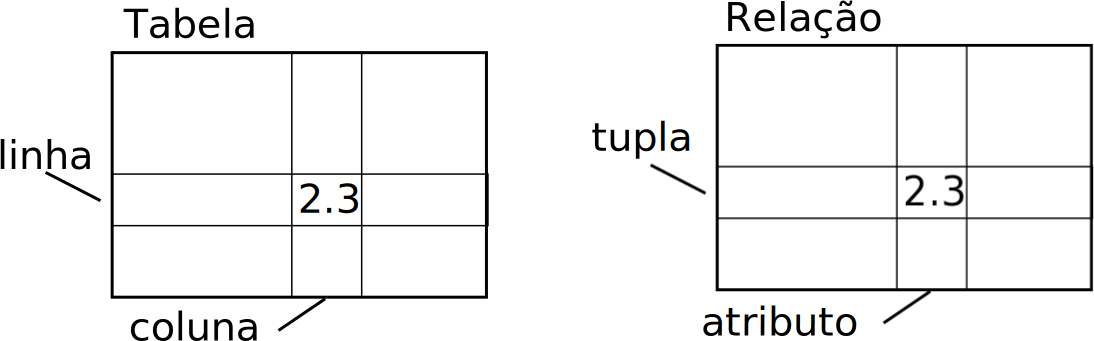
\includegraphics[height=1.50in]{figs2/relational.eps}}
\afterfig

%In technical descriptions of relational databases the concepts of 
%table, row, and column are more formally referred
%to as {\bf relation}, {\bf tuple}, and {\bf attribute}, respectively.
%We will use the less formal terms in this chapter.

Na descrição técnica de um banco de dados relacional o conceito de
tabela, linha e coluna são referências formais para {\bf relação},
{\bf tupla}, e {\bf atributo}, respectivamente.
Usaremos os termos menos formais neste capítulo.

%\section{SQLite manager Firefox add-on}
\section{Plugin do Firefox de Gerencia SQLite}
%While this chapter will focus on using Python to work with data 
%in SQLite database files, many operations can be done more
%conveniently using a Firefox add-on called the {\bf SQLite
%  Database Manager} which is freely available from:

O foco deste capítulo é o uso do Python para trabalhar com dados
com o SQLite, muitas operações podem ser feitas de forma mais
conveniente utilizando um {\it plugin} do Firefox, o {\bf SQLite
  Database Manager} que está disponível gratuitamente através do {\it link}:

\url{https://addons.mozilla.org/en-us/firefox/addon/sqlite-manager/}

%Using the browser you can easily create tables, insert data, edit data, 
%or run simple SQL queries on the data in the database.

Utilizando o navegador você pode facilmente criar tabelas, inserir, editar ou
executar consultas SQL nos dados da base de dados.

%In a sense, the database manager is similar to a text editor
%when working with text files.   When you want to do one or
%very few operations on a text file, you can just open it
%in a text editor and make the changes you want.   When you have 
%many changes that you need to do to a text file, often you 
%will write a simple Python program.  You will find the same 
%pattern when working with databases.  You will do simple
%operations in the database manager and more complex operations
%will be most conveniently done in Python.

De certa forma, o gerenciador de banco de dados é similar a um editor de texto
quando utilizado arquivos de texto. Quando você quer fazer uma ou mais
operações com um arquivo de texto, você pode simplesmente abrir o arquivo em
um editor de texto e fazer as alterações que desejar. Quando você tem que fazer
muitas alterações para fazer, normalmente você pode escrever um programa em
Python simples para executar esta tarefa. Você encontrará os mesmos padrões
quando for trabalhar com banco de dados. Você fará operações em um gerenciador
de banco de dados e as operações mais complexas serão mais convenientes se
forem feitas com Python.

%\section{Creating a database table}
\section{Criado uma tabela em um banco de dados}

%Databases require more defined structure than Python lists 
%or dictionaries\footnote{SQLite actually does allow some 
%flexibility in the type of data stored in a column,
%but we will keep our data types strict in this chapter
%so the concepts apply equally to other database systems 
%such as MySQL.}.

Bancos de dados precisam de estruturas mais bem definidas do quê listas ou
dicionários em Python\footnote{Atualmente o SQLite permite uma maior
  flexibilidade em relação aos tipos de dados que são armazenados em uma
  coluna, mas vamos manter os tipos de dados restritos neste capítulo, assim
  os mesmos conceitos aprendidos aqui podem ser aplicados a outros sistemas
  de banco de dados como MySQL.}.

%When we create a database {\bf table} we
%must tell the database in advance the names of each of the
%{\bf columns} in the table and the type of data which we are 
%planning to store in each {\bf column}.   When the database software
%knows the type of data in each column, it can choose the most 
%efficient way to store and look up the data based on the type of
%data.

Quando criamos uma {\bf tabela} em um banco de dados, precisamos informar ao
banco de dados previamente o nome de cada {\bf coluna} na tabela e o tipo de
dados que planejamos armazenar em cada {\bf coluna}. Quando o sistema de
banco de dados conhece o tipo de dado em cada coluna, ele pode definir a
forma mais eficiente de armazenar e consultar o dado baseado no tipo do dado.

%You can look at the various data types supported by SQLite
%at the following url:

Você pode visualizar os diversos tipos de dados que são suportados pelo SQLite
através do seguinte endereço:

\url{http://www.sqlite.org/datatypes.html}


%Defining structure for your data up front may seem inconvenient
%at the beginning, but the payoff is fast access to your data 
%even when the database contains a large amount of data.

Definir a estrutura dos seus tipos de dados pode parecer inconveniente no
começo, mas a recompensa é o acesso rápido aos dados mesmo quando o banco
de dados contém um grande número de informações.

%The code to create a database file and a table 
%named {\tt Tracks} with two columns in the 
%database is as follows:

O seguinte código cria um arquivo de banco de dados com uma tabela, chamada
{\tt Tracks} e com duas colunas:

\index{sqlite3 module}
\index{module!sqlite3}
\beforeverb
\begin{verbatim}
import sqlite3

conn = sqlite3.connect('music.sqlite3')
cur = conn.cursor()

cur.execute('DROP TABLE IF EXISTS Tracks ')
cur.execute('CREATE TABLE Tracks (title TEXT, plays INTEGER)')

conn.close()
\end{verbatim}
\afterverb
%
\index{connect function}
\index{function!connect}
\index{cursor function}
\index{function!cursor}
%The {\tt connect} operation makes a ``connection'' to the database 
%stored in the file {\tt music.sqlite3} in the current directory.   If
%the file does not exist, it will be created.  The reason this
%is called a ``connection'' is that sometimes the database is stored
%on a separate ``database server'' from the server on which we 
%are running our application.  In our simple examples 
%the database will just be a local file in the same directory
%as the Python code we are running.

A operação {\tt connect} cria uma ``conexão'' com o banco de dados armazenado
no arquivo {\tt music.sqlite3} no diretório corrente. Se o arquivo não
existir, este será criado. O motivo para isto ser chamado de ``conexão'' é
que algumas vezes o banco de dados está  em um ``servidor de banco de dados'' 
separado da aplicação propriamente dita. Em nossos exemplos o banco de dados
está armazenado localmente em um arquivo no mesmo diretório que o código
Python está sendo executado.


%A {\bf cursor} is like a file handle that we can use to perform
%operations on the data stored in the database.  Calling 
%{\tt cursor()} is very similar conceptually to calling
%{\tt open()} when dealing with text files.

Um {\bf cursos} é como um identificador de arquivo que podemos utilizar para
realizar operações sobre as informações armazenadas em um banco de dados. Ao
chamar a função {\tt cursor()}, conceitualmente, é similar ao chamar a função
{\tt open()} quando estamos trabalhando com arquivos de texto.

\beforefig
\centerline{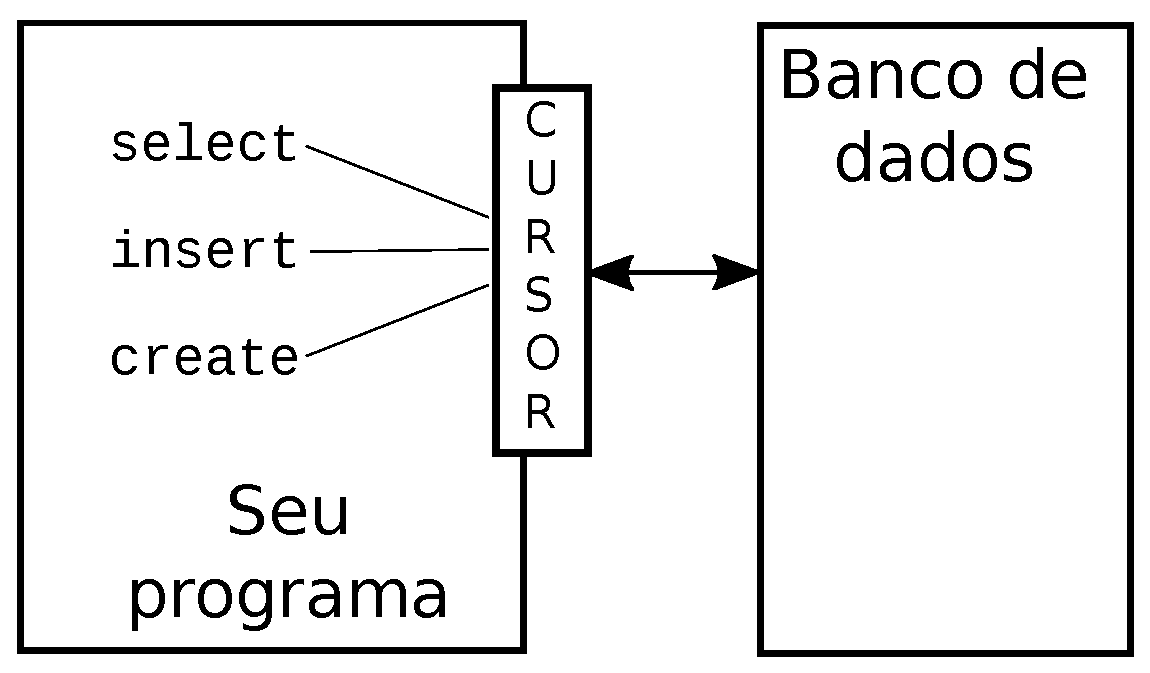
\includegraphics[height=1.50in]{figs2/cursor.eps}}
\afterfig

%Once we have the cursor, we can begin to execute 
%commands on the contents of the database using the {\tt execute()}
%method.

Uma vez que temos o cursos, podemos começar a executar comandos no conteúdo
armazenado no banco de dados utilizando o método {\tt execute()}.

%Database commands are expressed in a special language that has 
%been standardized across many different database vendors 
%to allow us to learn a single database language.   The database
%language is called {\bf Structured Query Language} or {\bf SQL}
%for short.

Os comandos de um banco de dados são expressos em uma linguagem especial que
foi padronizada por diferentes fornecedores de bancos de dados, que nos
permite aprender uma única linguagem. A linguagem dos bancos de dados é
chamada de {\bf Structured Query Language}\footnote{Em Português, pode ser
  chamada de Linguagem de Consulta Estruturada} ou referenciada pelo acrônimo
{\bf SQL}
\url{http://en.wikipedia.org/wiki/SQL}

%In our example, we are executing two SQL commands in our database.
%As a convention, we will show the SQL keywords in uppercase 
%and the parts of the command that we are adding (such as the
%table and column names) will be shown in lowercase.

Em nossos exemplos, estamos executando dois comandos SQL no banco de dados que
criamos. Convencionaremos que os comandos SQL serão mostrados em maiúsculas e
as partes que não são palavras reservadas do SQL (como os nomes das tabelas e
colunas) serão mostrados em minúsculas.

%The first SQL command removes the {\tt Tracks} table from the 
%database if it exists.  This pattern is simply to allow us to 
%run the same program to create the {\tt Tracks} table over 
%and over again without causing an error.  Note that the
%{\tt DROP TABLE} command deletes the table and all of its contents
%from the database (i.e., there is no ``undo'').

O primeiro comando SQL remove a tabela {\tt Tracks} do banco de dados se ela
existir. Este padrão nos permite executar o mesmo programa para criar a tabela
{\tt Tracks} repetidas vezes sem que cause erro. Perceba que o comando {\tt DROP
  TABLE} remove a tabela e todo o seu conteúdo do banco de dados (i.e., não é
possível desfazer esta operação)

\beforeverb
\begin{verbatim}
cur.execute('DROP TABLE IF EXISTS Tracks ')
\end{verbatim}
\afterverb
%
%The second command creates a table named
%{\tt Tracks} with a text column named {\tt title}
%and an integer column named {\tt plays}.
%
O segundo comando cria a tabela {\tt Tracks} com uma coluna chamada {\tt title}
com o tipo texto e uma coluna chamada {\tt plays} com o tipo inteiro.

\beforeverb
\begin{verbatim}
cur.execute('CREATE TABLE Tracks (title TEXT, plays INTEGER)')
\end{verbatim}
\afterverb
%
%Now that we have created a table named {\tt Tracks}, we can put some data
%into that table using the SQL {\tt INSERT} operation.   Again, we begin
%by making a connection to the database and obtaining the {\tt cursor}.
%We can then execute SQL commands using the cursor.
%
Agora que criamos a tabela {\tt Tracks}, podemos inserir algum dado dentro
dela utilizando a operação SQL {\tt INSERT}. Novamente, estamos
estabelecendo uma conexão com o banco de dados e obtendo o {\tt cursos}.
E então executamos o comando SQL utilizando o cursor.

%The SQL {\tt INSERT} command indicates which table we are using 
%and then defines a new row by listing the fields we want to 
%include {\tt (title, plays)} followed by the {\tt VALUES} we want
%placed in the new row.  We specify the values as question marks
%{\tt (?, ?)} to indicate that the actual values are passed in as a
%tuple {\tt ( 'My Way', 15 ) } as the second parameter to the
%{\tt execute()} call.

O comando SQL {\tt INSERT} indica qual tabela estamos utilizando, e em seguida, 
cria uma nova linha listando quais campos utilizaremos para incluir {\tt (title,
  plays)} seguido pelo comando {\tt VALUES} com os valores que desejamos
adicionar na nova linha. Especificamos os valores utilizando pontos de
interrogação {\tt (?, ?)} para indicar que os valores serão passados como
tuplas {\tt ( 'My Way', 15) } como um segundo parâmetro da chamada
{\tt execute()}.

\beforeverb
\begin{verbatim}
import sqlite3

conn = sqlite3.connect('music.sqlite3')
cur = conn.cursor()

cur.execute('INSERT INTO Tracks (title, plays) VALUES ( ?, ? )', 
    ( 'Thunderstruck', 20 ) )
cur.execute('INSERT INTO Tracks (title, plays) VALUES ( ?, ? )', 
    ( 'My Way', 15 ) )
conn.commit()

print 'Tracks:'
cur.execute('SELECT title, plays FROM Tracks')
for row in cur :
   print row

cur.execute('DELETE FROM Tracks WHERE plays < 100')
conn.commit()

cur.close()
\end{verbatim}
\afterverb
%
%First we {\tt INSERT} two rows into our table and use {\tt commit()} 
%to force the data to be written to the database file.

Primeiro nós adicionamos com {\tt INSERT} duas linha na nossa tabela e
usamos {\tt commit()} para forçar a escrita da informação no arquivo do banco
de dados.

\beforefig
\centerline{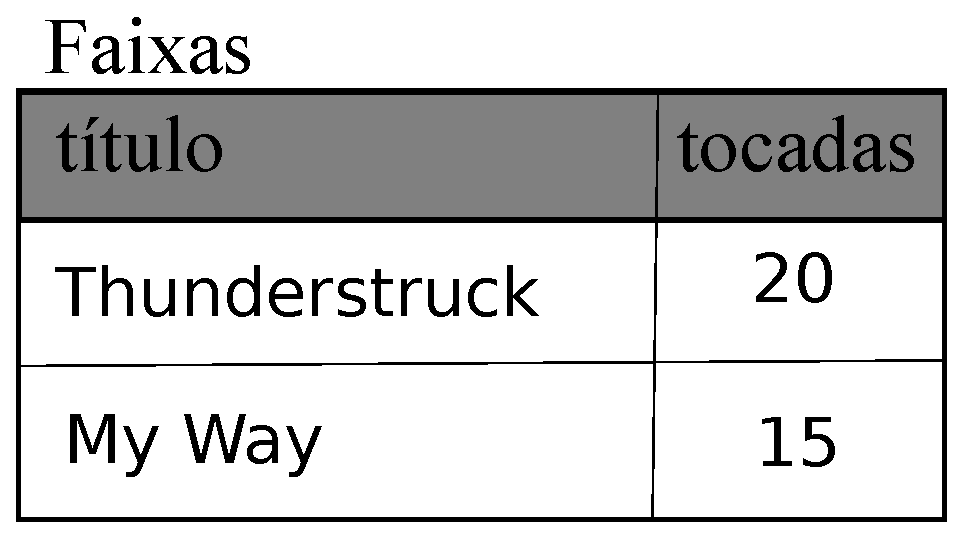
\includegraphics[height=1.00in]{figs2/tracks.eps}}
\afterfig

%Then we use the {\tt SELECT} command
%to retrieve the rows we just inserted from the table.  
%On the 
%{\tt SELECT} command, we indicate which columns we would like {\tt (title, plays)}
%and indicate which table we want to retrieve the data from.  After we 
%execute the {\tt SELECT} statement, the cursor is something we can loop through
%in a {\tt for} statement.   For efficiency,
%the cursor does not read all of the data from the
%database when we execute the {\tt SELECT} statement.  
%Instead, the data is read on demand
%as we loop through the rows in the {\tt for} statement.

Depois usamos o comando {\tt SELECT} para buscar a linha que acabamos de
inserir na tabela. Com o comando {\tt SELECT}, indicamos que coluna gostaríamos
{\tt (title, plays)} e de qual tabela queremos buscar a informação. Depois
de confirmar a executação do comando {\tt SELECT}, o cursor pode ser utilizado
como repetição através de um comando {\tt for}. Por questões de eficiência, o
cursor não lê toda a informação da base de dados quando executamos o comando
{\tt SELECT}. Ao invés disto, a informação é lida sob demanda enquanto
iteramos através da linha com o comando {\tt for}.

%The output of the program is as follows:

A saída do programa fica da seguinte forma:

\beforeverb
\begin{verbatim}
Tracks:
(u'Thunderstruck', 20)
(u'My Way', 15)
\end{verbatim}
\afterverb
%
\index{Unicode}
%Our {\tt for} loop finds two rows, and each row is a Python tuple with the
%first value as the {\tt title} and the second value as the number of {\tt plays}.
%Do not be concerned that the title strings are shown starting with 
%{\tt u'}.  This is an indication that the strings are {\bf Unicode} strings
%that are capable of storing non-Latin character sets.

A iteração do {\tt for} encontrou duas linhas, e cada linha é uma tupla em
Python com o primeiro valor como {\tt title} e o segundo como o número de
{\tt plays}. Não se preocupe com o fato de a {\it strings} são mostrados com
o caractere {\tt u'} no começo. Isto é uma indicação que a {\it string} estão
em {\bf Unicode}, o que indica que são capazes de armazenar um conjunto de
caractere não-Latin.

%At the very end of the program, we execute an SQL command to {\tt DELETE} 
%the rows we have just created so we can run the program over and over.
%The {\tt DELETE} command shows the use of a {\tt WHERE} clause that
%allows us to express a selection criterion so that we can ask the database
%to apply the command to only the rows that match the criterion.  In this example
%the criterion happens to apply to all the rows so we empty the table
%out so we can run the program repeatedly.  After the {\tt DELETE} is performed,
%we also call {\tt commit()} to force the data to be removed from the database.

No final do programa, executamos o comando SQL {\tt DELETE} para remover as
linhas que acabamos de criar, assim podemos executar o programa repetidas
vezes. O {\tt DELETE} pode ser utilizado com a condição {\tt WHERE} que permite
selecionar através de uma expressão o critério permitindo pesquisar no banco
de dados somente as linhas que correspondem com a expressão utilizada. Neste
exemplo a expressão construida se aplica em todas as linhas, para que possamos
executar o programa outras vezes. Depois de executar o {\tt DELETE} chamamos o
{\tt commit()} para forçar que o dado seja removido do banco de dados.

%\section{Structured Query Language summary}
\section{Resumo de Structured Query Language (SQL)}

%So far, we have been using the Structured Query Language in our Python
%examples and have covered many of the basics of the SQL commands.
%In this section, we look at the SQL language in particular
%and give an overview of SQL syntax.

Estamos utilizando SQL junto com os exemplos de Python e até agora cobrimos
muitos comandos SQL básicos. Nesta seção, vamos olhar a linguagem SQL com
mais atenção e apresentaremos uma visão geral da sintaxe do SQL.

%Since there are so many different database vendors, the Structured Query
%Language (SQL) was standardized so we could communicate in a portable
%manner to database systems from multiple vendors.

Existem diferentes fornecedores de bancos de dados, a linguagem SQL foi
padronizada, desta forma podemos nos comunicar de maneira portável entre os
diferentes sistemas de banco de dados dos diferentes fornecedores.

%A relational database is made up of tables, rows, and columns.  The columns
%generally have a type such as text, numeric, or date data.  When we create
%a table, we indicate the names and types of the columns:

Basicamente um banco de dados relacional é composto por tabelas, linhas e
colunas. As colunas geralmente possuem tipos, como textos, números ou
informação de data. Quando criamos uma tabela, indicamos os nomes e tipos das
colunas:

\beforeverb
\begin{verbatim}
CREATE TABLE Tracks (title TEXT, plays INTEGER)
\end{verbatim}
\afterverb
%
%To insert a row into a table, we use the SQL {\tt INSERT} command:
%
Para inserir uma linha em uma tabela, utilizamos o comando SQL {\tt INSERT}:

\beforeverb
\begin{verbatim}
INSERT INTO Tracks (title, plays) VALUES ('My Way', 15)
\end{verbatim}
\afterverb
%
%The {\tt INSERT} statement specifies the table name, then a list of
%the fields/columns that you would like to set in the new row, and then 
%the keyword {\tt VALUES} and a list of corresponding values 
%for each of the fields.
%
A declaração do {\tt INSERT} especifica o nome da tabela, e então, uma lista
dos campos/colunas que gostaríamos de definir na nova linha, e por fim,
através do campo {\tt VALUES} passamos uma lista de valores correspondentes a
cada campo.

%The SQL {\tt SELECT} command is used to retrieve rows and columns from a database.
%The {\tt SELECT} statement lets you specify which columns you would
%like to retrieve as well as a {\tt WHERE} clause to select which 
%rows you would like to see.  It also allows an optional 
%{\tt ORDER BY} clause to control the sorting of the returned rows.

O comando {\tt SELECT} é utilizado para buscar as linhas e colunas de um banco
de dados. A declaração do {\tt SELECT} permite que você especifique qual coluna
gostaria de buscar, bem como utilizando a condição do {\tt WHERE}, permite
selecionar qual linha gostaríamos de visualizar. Isto também possibilita o uso
de uma condição opcional, {\tt ORDER BY}, para ordenar as linhas retornadas.

\beforeverb
\begin{verbatim}
SELECT * FROM Tracks WHERE title = 'My Way'
\end{verbatim}
\afterverb
%
%Using \verb"*" indicates that you want the database to return all of 
%the columns for each row that matches the {\tt WHERE} clause.

O uso do \verb"*" indica que o banco de dados deve retornar todas as colunas
para cada linha que casa com a condição {\tt WHERE}.

%Note, unlike in Python, in a SQL {\tt WHERE} clause 
%we use a single equal sign 
%to indicate a test for equality rather than a double equal sign.
%Other logical operations allowed in a {\tt WHERE} clause include

Atenção, diferente de Python, a condição {\tt WHERE}, em SQL, utiliza o sinal
de igual simples (\verb"="), para indicar uma condição de igualdade, ao invés de
um sinal duplo (\verb"==")
\verb"<",
\verb">",
\verb"<=",
\verb">=",
\verb"!=",
%as well as {\tt AND} and {\tt OR} and parentheses
%to build your logical expressions.

assim como é possível utilizar as condições {\tt AND} e {\tt OR} e parênteses
para construir expressões lógicas.

%You can request that the returned rows be sorted by one of 
%the fields as follows:

Você pode pedir que as linhas retornadas sejam ordenadas por um dos campos
como apresentados no exemplo a seguir:
\beforeverb
\begin{verbatim}
SELECT title,plays FROM Tracks ORDER BY title
\end{verbatim}
\afterverb
%
%To remove a row, you need a {\tt WHERE} clause on an SQL {\tt DELETE}
%statement.  The {\tt WHERE} clause determines which rows are to be deleted:
%
Para remover uma linha, é preciso combinar a condição {\tt WHERE} com a
condição {\tt DELETE}. O {\tt WHERE} irá determinar quais linhas serão
removidas:

\beforeverb
\begin{verbatim}
DELETE FROM Tracks WHERE title = 'My Way'
\end{verbatim}
\afterverb
%
%It is possible to {\tt UPDATE} a column or columns within one or more rows
%in a table using the SQL {\tt UPDATE} statement as follows:
%
É possível alterar/atualizar uma ou mais colunas e suas linhas de uma tabela
utilizando a condição SQL {\tt UPDATE}, da seguinte forma:

\beforeverb
\begin{verbatim}
UPDATE Tracks SET plays = 16 WHERE title = 'My Way'
\end{verbatim}
\afterverb
%
%The {\tt UPDATE} statement specifies a table and 
%then a list of fields and values to change after the {\tt SET} 
%keyword and then an optional {\tt WHERE} clause to select
%the rows that are to be updated.  A single {\tt UPDATE} statement
%will change all of the rows that match the {\tt WHERE} clause.  If 
%a {\tt WHERE} clause is not specified, it performs the {\tt UPDATE}
%on all of the rows in the table.
%
A condição {\tt UPDATE} especifica uma tabela e depois uma lista de campos e
valores que serão alterados após o comando {\tt SET}, e utilizando uma condição
{\tt WHERE}, opctional, é possível selecionar as linhas que serão atualizadas.
Uma condição {\tt UPDATE} irá mudar todas as linhas que casam com a condição
{\tt WHERE}. Se a condição {\tt WHERE} não for especificada, o {\tt UPDATE}
será aplicado em todas as linhas da tabela.

%These four basic SQL commands (INSERT, SELECT, UPDATE, and DELETE) allow 
%the four basic operations needed to create and maintain data.

Os quatros comandos básicos de SQL (INSERT, SELECT, UPDTE e DELETE) permitem
as quatro operações básicas necessárias para criação e manutenção das
informações em um banco de dados.

%\section{Spidering Twitter using a database}
\section{Rastreando o Twitter utilizando um banco de dados}

%In this section, we will create a simple spidering program that will 
%go through Twitter accounts and build a database of them.
%\emph{Note: Be very careful when running this program.  You do not
%want to pull too much data or run the program for too long and
%end up having your Twitter access shut off.}

Nesta seção criaremos um programa simples para rastreamento que navegará
através de contas de usuários do Twitter e construirá um banco de dados
destas referentes as estes usuários.
\emph{Nota: Tenha muito cuidado ao executar este programa. Você não irá querer
  extrair muitas informações ou executar o programa por muito tempo e acabar
  tendo sua conta do Twitter bloqueada.}

%One of the problems of any kind of spidering program is that it 
%needs to be able to be stopped and restarted many times and 
%you do not want to lose the data that you have retrieved so far.
%You don't want to always restart your data retrieval at the
%very beginning so we want to store data as we retrieve it so our
%program can start back up and pick up where it left off.

Um dos problemas, em qualquer tipo de programas de rastreamento, é que precisa
ser capaz de ser interrompido e reiniciado muitas vezes e você não quer perder
informações que você já tenha recuperado até agora. Não quer sempre reiniciar
a recuperação dos dados desde o começo, então armazenamos as informações tão
logo seja recuperada, assim o programa poderá reiniciar a busca do ponto onde
parou.


%We will start by retrieving one person's Twitter friends and their
%statuses, looping through the list of friends, and adding each 
%of the friends to a database to be retrieved in the future.  After
%we process one person's Twitter friends, we check in our database
%and retrieve one of the friends of the friend.  We do this over and
%over, picking an ``unvisited'' person, retrieving their friend list,
%and adding friends we have not seen to our list for a future visit.

Vamos começar recuperando os amigos de uma pessoa no Twitter e seus status,
iterando na lista de amigos, e adicionando cada um ao banco de dados para
que possa ser recuperado no futuro. Depois de listar os amigos de uma pessoa,
verificamos na nossa base de dados e coletamos os amigos de um dos amigos da
primeira pessoa. Vamos fazendo isto repetidas vezes, escolhendo umas das
pessoas ``não visitadas'', recuperando sua lista de amigos, e
adicionando amigos que não tenhamos visto anteriormente a nossa lista, para
visitar futuramente.

%We also track how many times we have seen a particular friend in the
%database to get some sense of their ``popularity''.

Também rastrearemos quantas vezes vimos um amigo em particular na nossa base
para ter uma ideia da sua ``popularidade''.

%By storing our list of known accounts and whether 
%we have retrieved the account or not, 
%and how popular the account is in a database on the disk
%of the computer, we can stop and
%restart our program as many times as we like.

Armazenando nossa lista de contas conhecidas, no banco de dados no disco do
nosso computador, e se já recuperamos a conta ou não, e quanto esta conta é
popular, podemos parar e recomeçar nosso programa quantas vezes quisermos.

% TODO: Add a reference to the right spot
%This program is a bit complex. It is based on the code 
%from the exercise earlier in the book that uses
%the Twitter API.

% TODO: Adicionar a referência do código para o lugar certo.
Este programa é um pouco complexo. É baseado em um exercício apresentado
anteriormente neste livro, que utiliza a API do Twitter

%Here is the source code for our Twitter spidering application:

O seguinte código apresenta o programa que realiza o rastreamento no Twitter:

\beforeverb
\begin{verbatim}
import urllib
import twurl
import json
import sqlite3

TWITTER_URL = 'https://api.twitter.com/1.1/friends/list.json'

conn = sqlite3.connect('spider.sqlite3')
cur = conn.cursor()

cur.execute('''
CREATE TABLE IF NOT EXISTS Twitter 
(name TEXT, retrieved INTEGER, friends INTEGER)''')

while True:
    acct = raw_input('Enter a Twitter account, or quit: ')
    if ( acct == 'quit' ) : break
    if ( len(acct) < 1 ) :
        cur.execute('SELECT name FROM Twitter WHERE retrieved = 0 LIMIT 1')
        try:
            acct = cur.fetchone()[0]
        except:
            print 'No unretrieved Twitter accounts found'
            continue

    url = twurl.augment(TWITTER_URL, 
               {'screen_name': acct, 'count': '20'} )
    print 'Retrieving', url
    connection = urllib.urlopen(url)
    data = connection.read()
    headers = connection.info().dict
    # print 'Remaining', headers['x-rate-limit-remaining']
    js = json.loads(data)
    # print json.dumps(js, indent=4)

    cur.execute('UPDATE Twitter SET retrieved=1 WHERE name = ?', (acct, ) )

    countnew = 0
    countold = 0
    for u in js['users'] :
        friend = u['screen_name']
        print friend
        cur.execute('SELECT friends FROM Twitter WHERE name = ? LIMIT 1', 
            (friend, ) )
        try:
            count = cur.fetchone()[0]
            cur.execute('UPDATE Twitter SET friends = ? WHERE name = ?', 
                (count+1, friend) )
            countold = countold + 1
        except:
            cur.execute('''INSERT INTO Twitter (name, retrieved, friends) 
                VALUES ( ?, 0, 1 )''', ( friend, ) )
            countnew = countnew + 1
    print 'New accounts=',countnew,' revisited=',countold
    conn.commit()

cur.close()
\end{verbatim}
\afterverb
%
%Our database is stored in the file {\tt spider.sqlite3} and it has one 
%table named {\tt Twitter}.  Each row in the {\tt Twitter} table
%has a column for the account name, whether we have retrieved the friends
%of this account, and how many times this account has been ``friended''.

%
Nossa base de dados está armazenada no arquivo {\tt spider.sqlite3} e possui
uma tabela chamada {\tt Twitter}. Cada linha na tabela {\tt Twitter} tem uma
coluna para o nome da conta, se recuperamos os amigos desta conta, e quantas
vezes esta conta foi ``seguido''.

%In the main loop of the program, we prompt the user for a Twitter
%account name or ``quit'' to exit the program.  
%If the user enters a Twitter account, we retrieve the 
%list of friends and statuses
%for that user and add each friend to the database if 
%not already in the database.  If the friend is already in the list, 
%we add 1 to the {\tt friends} field in the row in the database.

Na repetição principal do programa, perguntamos ao usuário uma conta de Twitter
ou ``quit'' para sair do programa. Se o usuário informar um usuário do Twitter,
o programa começa a recuperar a lista de amigos e os status para aquele
usuário e adiciona cada amigo na base de dados se não possuir. Se o amigo já
está na lista, nós adicionamos ``1'' no campo {\tt friends} da base de dados.


%If the user presses enter, we look in the database for the next 
%Twitter account that we have not yet retrieved, retrieve the
%friends and statuses for that account, add them to the database 
%or update them, and increase their {\tt friends} count.

Se o usuário pressionar {\tt enter}, pesquisamos na base a próxima conta que
não rastreamos ainda, e então rastreamos os amigos e status com aquela conta
e adicionamos na base de dados ou atualizamos, incrementando seu contador de
{\tt friends}.

%Once we retrieve the list of friends and statuses, we loop 
%through all of the {\tt user} items in the returned JSON
%and retrieve the \verb"screen_name" for each user.  Then we use
%the {\tt SELECT} statement to see if we already have stored this
%particular \verb"screen_name" in the database and retrieve the
%friend count ({\tt friends}) if the record exists.

Uma vez que rastreamos a lista de amigos e status, iteramos entre todas os
ítens {\tt user} retornados no JSON e rastreamos o  \verb"screen_name" para
cada usuário. Então utilizamos a declaração {\tt SELECT} para ver se já
armazenamos este \verb"screen_name" em particular na base e recuperamos o
contador de amigos ({\tt friends}), se este registro existir.

\beforeverb
\begin{verbatim}
    countnew = 0
    countold = 0
    for u in js['users'] :
        friend = u['screen_name']
        print friend
        cur.execute('SELECT friends FROM Twitter WHERE name = ? LIMIT 1', 
            (friend, ) )
        try:
            count = cur.fetchone()[0]
            cur.execute('UPDATE Twitter SET friends = ? WHERE name = ?', 
                (count+1, friend) )
            countold = countold + 1
        except:
            cur.execute('''INSERT INTO Twitter (name, retrieved, friends) 
                VALUES ( ?, 0, 1 )''', ( friend, ) )
            countnew = countnew + 1
    print 'New accounts=',countnew,' revisited=',countold
    conn.commit()
\end{verbatim}
\afterverb
%
%Once the cursor executes the {\tt SELECT} statement, 
%we must retrieve the rows.  We could do this with a {\tt for} 
%statement, but since we are only retrieving
%one row ({\tt LIMIT 1}), we can use the {\tt fetchone()} method to fetch the
%first (and only) row that is the result of the {\tt SELECT} operation.  
%Since {\tt fetchone()} returns the row as a {\bf tuple} (even though there is only
%one field), we take the first value from the tuple using {\tt [0]} to get the 
%current friend count into the variable {\tt count}.  

%
Uma vez que o cursor tenha executado o {\tt SELECT}, nós devemos recuperar as
linhas. Podemos fazer isto com uma declaração de {\tt for}, mas uma vez que
estamos recuperando uma linha ({\tt LIMIT 1}), podemos utilizar o método
{\tt fetchone()} para buscar a primeira (e única) linha que é o resultado da
operação {\tt SELECT}. Sendo o retorno {\tt fetchone()} uma linha como uma
{\bf tupla} (ainda que haja somente um campo), pegamos o primeiro valor da
tupla utilizando índice {\tt [0]} para pegar o contador de amigos atual dentro
da variável {\tt count}.

%If this retrieval is successful, we use the SQL {\tt UPDATE} statement with a 
%{\tt WHERE} clause to add 1 to the {\tt friends} column for the row that 
%matches the friend's account.  Notice that there are two placeholders (i.e.,
%question marks) in the SQL, and the second parameter to the {\tt execute()} is
%a two-element tuple that holds the values to be substituted into the SQL
%in place of the question marks.

Se a busca for bem sucedida, utilizamos a declação {\tt UPDATE} com a clausula 
{\tt WHERE} para adicionar 1 na coluna {\tt friends} para a linha que
corresponde com a conta do amigo. Note que existem dois espaços reservados
(i.e., pontos de interrogações) no SQL, e o segundo parâmetro para o
{\tt execute()} é uma tupla que armazena o valor para substituir no SQL no
lugar dos pontos de interrogações.

%If the code in the {\tt try} block fails, it is probably because no record
%matched the {\tt WHERE name = ?} clause on the SELECT statement.  So in the
%{\tt except} block, we use the SQL {\tt INSERT} statement to add the friend's
%\verb"screen_name" to the table with an indication that we have not yet 
%retrieved the \verb"screen_name" and set the friend count to zero.

Se o bloco {\tt try} falhar, é provavelmente por que nenhum resultado
corresponde a clausula em {\tt WHERE name = ?} do SELECT. Então no block
{\tt except}, utilizamos a declaração {\tt INSERT} para adicionar o
\verb"screen_name" do amigo a tabela com a indicação que ainda não rastreamos
o \verb"screen_name" e setamos o contador de amigos com 0 (zero).

%So the first time the program runs and we enter a Twitter account, the program
%runs as follows:

Assim, a primeira vez que o programa é executado e informamos uma conta do
Twitter, a saída do programa é a seguinte:

\beforeverb
\begin{verbatim}
Enter a Twitter account, or quit: drchuck
Retrieving http://api.twitter.com/1.1/friends ...
New accounts= 20  revisited= 0
Enter a Twitter account, or quit: quit
\end{verbatim}
\afterverb
%
%Since this is the first time we have run the program, the database
%is empty and we create the database in the file {\tt spider.sqlite3} and
%add a table named {\tt Twitter} to the database.  Then we retrieve
%some friends and add them all to the database since the database is
%empty.

Como esta é a primeira vez que executamos o programa, o banco de dados está
vazio e criamos o banco no arquivo {\tt spider.sqlite3}, adicionamos a tabela
chamada {\tt Twitter} na base de dados. Então nós rastreamos alguns amigos e
os adicionamos a base, uma vez que ela está vazia.

%At this point, we might want to write a simple database dumper
%to take a look at what is in our {\tt spider.sqlite3} file:

Neste ponto podemos escrever um {\it dumper} simples para olhar o que está no
nosso arquivo {\tt spider.sqlite3}:

\beforeverb
\begin{verbatim}
import sqlite3

conn = sqlite3.connect('spider.sqlite3')
cur = conn.cursor()
cur.execute('SELECT * FROM Twitter')
count = 0
for row in cur :
   print row
   count = count + 1
print count, 'rows.'
cur.close()
\end{verbatim}
\afterverb
%
%This program simply opens the database and selects all of the 
%columns of all of the rows in the table {\tt Twitter}, then 
%loops through the rows and prints out each row.

%
Este programa abre o banco de dados e seleciona todas as colunas de todas as
linhas na tabela {\tt Twitter}, depois itera em cada linha e imprime o valor
dentro de cada uma.

%If we run this program after the first execution of our Twitter
%spider above, its output will be as follows:

Se executarmos este programa depois da primeira execução do nosso rastreador
{\it spider} do Twitter, sua saída será como a seguinte:

\beforeverb
\begin{verbatim}
(u'opencontent', 0, 1)
(u'lhawthorn', 0, 1)
(u'steve_coppin', 0, 1)
(u'davidkocher', 0, 1)
(u'hrheingold', 0, 1)
...
20 rows.
\end{verbatim}
\afterverb
%
%We see one row for each \verb"screen_name", that we 
%have not retrieved the data for that \verb"screen_name", and 
%everyone in the database has one friend.

%
Veremos uma linha para cada \verb"screen_name", que não tenhamos recuperado
o dado daquele \verb"screen_name", e todos tem um amigo.

%Now our database reflects the retrieval of the friends of 
%our first Twitter account ({\bf drchuck}).  We can run the program
%again and tell it to retrieve the friends of the next 
%``unprocessed'' account by simply pressing enter instead of
%a Twitter account as follows:

Agora nosso banco de dados reflete quais amigos estão relacionados com a nossa
primeira conta do Twitter ({\bf drchuck}) utilizada para rastreamento. Podemos
executar o programa novamente e mandar rastrear a próxima conta
``não processada'' e recuperar os amigos, simplemente pressionando {\tt enter}
ao invés de informar uma conta do Twitter, conforme o exemplo a seguir:


\beforeverb
\begin{verbatim}
Enter a Twitter account, or quit: 
Retrieving http://api.twitter.com/1.1/friends ...
New accounts= 18  revisited= 2
Enter a Twitter account, or quit: 
Retrieving http://api.twitter.com/1.1/friends ...
New accounts= 17  revisited= 3
Enter a Twitter account, or quit: quit
\end{verbatim}
\afterverb
%
%Since we pressed enter (i.e., we did not specify a Twitter account),
%the following code is executed:

%
Uma vez que pressionamos {\tt enter} (i.e., não especificamos uma conta do
Twitter), o seguinte código é executado:

\beforeverb
\begin{verbatim}
    if ( len(acct) < 1 ) :
        cur.execute('SELECT name FROM Twitter WHERE retrieved = 0 LIMIT 1')
        try:
            acct = cur.fetchone()[0]
        except:
            print 'No unretrieved twitter accounts found'
            continue
\end{verbatim}
\afterverb
%
%We use the SQL {\tt SELECT} statement to retrieve the name of the first 
%({\tt LIMIT 1}) user who still has their ``have we retrieved this user''
%value set to zero.  We also use the {\tt fetchone()[0]} pattern within 
%a try/except block to either extract a \verb"screen_name" from the retrieved
%data or put out an error message and loop back up.

%
Utilizamos a declaração SQL {\tt SELECT} para recuperar o nome do primeiro
({\tt LIMIT 1}) usuário que ainda tem seu ``recuperamos este usuário'' com o
valor setado em zero. Também utilizamos o padrão {\tt fetchone()[0]} dentro de
um bloco try/except para extrair também um \verb"screen_name" do dado
recuperado ou apresentamos uma mensagem de erro e iteramos novamente.

%If we successfully retrieved an unprocessed \verb"screen_name", we retrieve
%their data as follows:

Se tivermos sucesso ao recuperar um \verb"screen_name" não processado, vamos
extrair seus dados da seguinte maneira:

\beforeverb
\begin{verbatim}
    url = twurl.augment(TWITTER_URL, {'screen_name': acct, 'count': '20'} )
    print 'Retrieving', url
    connection = urllib.urlopen(url)
    data = connection.read()
    js = json.loads(data)

    cur.execute('UPDATE Twitter SET retrieved=1 WHERE name = ?', (acct, ) )
\end{verbatim}
\afterverb
%
%Once we retrieve the data successfully, we use the {\tt UPDATE} statement 
%to set the {\tt retrieved} column to 1 to indicate that we have completed 
%the retrieval of the friends of this account.  This keeps us from retrieving
%the same data over and over and keeps us progressing forward through the network
%of Twitter friends.
%
Ao recuperar os dados com sucesso, utilizaremos a declaração {\tt UPDATE} para
setar a coluna {\tt retrieved} para 1 para indicar que completamos a extração
dos amigos relacionados com esta conta. Isto no permite recuperar o mesmo dado
diversas vezes e nos permite prosseguir através da lista de amigos no Twitter. 

%If we run the friend program and press enter twice to retrieve the next 
%unvisited friend's friends,
%then run the dumping program, it will give us the following output:

Se executarmos o programa novamente, e pressionarmos {\tt enter} duas vezes
seguidas para recuperar os próximos amigos do amigo e depois executarmos o
programa de {\it dumping}, ele nos mostrará a seguinte saída:

\beforeverb
\begin{verbatim}
(u'opencontent', 1, 1)
(u'lhawthorn', 1, 1)
(u'steve_coppin', 0, 1)
(u'davidkocher', 0, 1)
(u'hrheingold', 0, 1)
...
(u'cnxorg', 0, 2)
(u'knoop', 0, 1)
(u'kthanos', 0, 2)
(u'LectureTools', 0, 1)
...
55 rows.
\end{verbatim}
\afterverb
%
%We can see that we have properly recorded that we have visited 
%{\tt lhawthorn} and {\tt opencontent}.  Also the accounts 
%{\tt cnxorg} and {\tt kthanos} already have two followers.
%Since we now have retrieved the friends of three people
%({\tt drchuck}, {\tt opencontent}, and {\tt lhawthorn}) our table has 55 rows 
%of friends to retrieve.

Podemos ver que gravamos de forma apropriada que visitamos os usuários
{\tt lhawthorn} e {\tt opencontent}. E que as contas {\tt cnxorg} e
{\tt kthanos} já tem dois seguidores. Desde que tenhamos recuperado os amigos
de três pessoas ({\tt drchuck}, {\tt opencontent}, e {\tt lhawthorn}) nossa
tabela tem agora 55 linhas de amigos recuperados.

%Each time we run the program and press enter it will pick the next 
%unvisited account (e.g., the next account will be \verb"steve_coppin"),
%retrieve their friends, mark them as retrieved, and for each of the 
%friends of \verb"steve_coppin" either add them to the end of the 
%database or update their friend count if they are already in the
%database.

Cada vez que executamos o programa e pressionamos {\tt enter} ele pegará a
próxima conta não visitada (e.g., a próxima conta será \verb"steve_coppin"),
recuperar seus amigos, marcá-los como recuperados, e para cada um dos amigos
de \verb"steve_coppin" também adicionaremos eles para no fim da base de dados 
e atualizaremos seus amigos que já estiverem na base de dados.

%Since the program's data is all stored on disk in a database, 
%the spidering activity can be suspended and resumed as many times as you 
%like with no loss of data.

Assim que os dados do programa estejam armazenados no disco em um banco de
dados o rastreamento pode ser suspenso e reiniciado tantas vezes quando
quiser sem a perda de informações.

%\section{Basic data modeling}
\section{Modelagem de dados básica}

%The real power of a relational database is when we create multiple tables
%and make links between those tables.   The act of deciding how to break
%up your application data into multiple tables and establishing the
%relationships between the tables is called {\bf data modeling}.  The
%design document that shows the tables and their relationships 
%is called a {\bf data model}.

O verdadeiro poder de um banco de dados relacional é quando criamos múltiplas
tabelas e criamos ligações entre elas. Decidir como dividir os dados da sua
aplicação em diferentes tabelas e estabelecer a relação entre estas tabelas é
o que chamamos de {\bf modelagem de dados}. O documento que mostra a estrutura 
das tabelas e suas relações é chamado de {\bf modelo de dados}.

%Data modeling is a relatively sophisticated skill and we will only introduce
%the most basic concepts of relational data modeling in this section.  For more
%detail on data modeling you can start with:

Modelagem de dados é uma habilidade relativamente sofisticada e nesta seção
nós iremos somente introduzir os conceitos mais básicos da modelagem de dados
relacionais. Para maiores detalhes sobre modelagem de dados você pode começar
com:

\url{http://en.wikipedia.org/wiki/Relational_model}

%Let's say for our Twitter spider application, instead of just
%counting a person's friends, we wanted to keep a list of 
%all of the incoming relationships so we could find a list of 
%everyone who is following a particular account.

Digamos que para a nossa aplicação de rastreamento do Twitter, ao invés de
só contar os amigos das pessoas, nós queiramos manter uma lista de todas as
relações de entrada, então poderemos encontrar uma lista de todos que seguem
uma pessoa em particular.

%Since everyone will potentially have many accounts that follow
%them, we cannot simply add a single column to our {\tt Twitter} table. 
%So we create a new table that keeps track of pairs of friends.
%The following is a simple way of making such a table:

Já que todos, potencialmente, terão tantas contas que o sigam, nós não podemos
simplesmente adicionar uma coluna para nossa tabela {\tt Twitter}. Então
criamos uma nova tabela que mantém o controle dos pares de amigos. A seguir
temos uma forma simples de criar tal tabela:

\beforeverb
\begin{verbatim}
CREATE TABLE Pals (from_friend TEXT, to_friend TEXT)
\end{verbatim}
\afterverb
%
%Each time we encounter a person who {\tt drchuck} is following, we
%would insert a row of the form:
%
Toda vez que encontrarmos uma pessoa que {\tt drchuck} está seguindo, nós
iremos inserir uma linha da seguinte forma:

\beforeverb
\begin{verbatim}
INSERT INTO Pals (from_friend,to_friend) VALUES ('drchuck', 'lhawthorn')
\end{verbatim}
\afterverb
%
%As we are processing the 20 friends from the {\tt drchuck}
%Twitter feed, we will insert 20 records with ``drchuck''
%as the first parameter so we will end up duplicating the 
%string many times in the database.
%
Como estamos processando 20 amigos da conta do {\it Twitter} do {\tt drchuck},
inserimor 20 registros com ``drchuck'' como primeiro parâmetro e assim
acaberemos duplicando a {\it string} muitas vezes no banco de dados.

%This duplication of string data violates one of the best practices 
%for {\bf database normalization} which basically states that
%we should never put the same string data in the database more than once.  
%If we need the data more than once, we create a 
%numeric {\bf key} for the data and reference the actual data 
%using this key.

Esta duplicação de dados viola uma das melhores práticas da {\bf normatização
  de banco de dados} que basicamente afirma que nunca devemos colocar o mesmo
dado mais de uma vez em um banco de dados. Se precisarmos inserir um dado mais
de uma vez, criamos uma referência numérica {\bf key} (chave) para o dado, e
utilizamos a chave para referenciar o dado.

%In practical terms, a string takes up a lot more 
%space than an integer on the disk
%and in the memory of our computer, and takes more processor time
%to compare and sort.  If we only have a few hundred entries, 
%the storage and processor time hardly matters.  But if we have 
%a million people in our database and a possibility of 100 million
%friend links, it is important to be able to scan data as quickly
%as possible.

Na prática, uma {\it string} ocupa muito mais espaço do que um inteiro, no
disco e na memória do nosso computador, e leva mais tempo do processor para
comparar e ordenar. Se tivermos somente algumas centenas de entradas, a base
de dados e o tempo de processamento dificilmente importarão. Mas se tivermos
um milhão de pessoas na nossa base de dados e uma possibilidade de 100 milhões
de conexões de amigos, é importante permitir examinar os dados o mais rápido
possível.

%We will store our Twitter accounts in a table named {\tt People}
%instead of the {\tt Twitter} table used in the previous example.
%The {\tt People} table has an additional column 
%to store the numeric key associated with the 
%row for this Twitter user.   
%SQLite has a feature that automatically adds the key value
%for any row we insert into a table using a special type of 
%data column ({\tt INTEGER PRIMARY KEY}).

Nós armazenaremos nossas contas do Twitter em uma tabela chamada {\tt People}
ao invés de utilizar a tabela {\tt Twitter} utilizada no exemplo anterior. A
tabela {\tt People} tem uma coluna adicional para armazenar uma chave associada
a linha para este usuário.

%We can create the {\tt People} table with this additional 
%{\tt id} column as follows:

Podemos criar a tabela {\tt People} com esta coluna {\tt id} adicional com o
seguinte comando:

\beforeverb
\begin{verbatim}
CREATE TABLE People 
    (id INTEGER PRIMARY KEY, name TEXT UNIQUE, retrieved INTEGER)
\end{verbatim}
\afterverb
%
%Notice that we are no longer maintaining a friend count in each row
%of the {\tt People} table.
%When we select {\tt INTEGER PRIMARY KEY} as the type of our {\tt id} column,
%we are indicating that we would like SQLite to manage this column and 
%assign a unique numeric key to each row we insert automatically.
%We also add the keyword {\tt UNIQUE} to indicate that we will not 
%allow SQLite to insert two rows with the same value for {\tt name}.
%
Perceba que nós não estamos mais mantendo uma conta de amigo em cada linha da
tabela {\tt People}. Quando selecionamos {\tt INTEGER PRIMARY KEY} como o tipo
da nossa coluna {\tt id}, estamos indicando que gostaríamos que o SQLite
gerencie esta coluna e defina uma chave numérica única automagicamente para
cada linha que inserirmos. Também adicionamos uma palavra-chave {\tt UNIQUE}
para indicar que não permitiremos ao SQLite inserir duas linhas com o mesmo
valor para {\tt name}.

%Now instead of creating the table {\tt Pals} above, we create
%a table called {\tt Follows} with two integer columns
%\verb"from_id" and \verb"to_id" and a constraint on the table that
%the \emph{combination} of \verb"from_id" and \verb"to_id" must be unique 
%in this table (i.e., we cannot insert duplicate rows) in our database.

Agora, ao invés de criar a tabela {\tt Pals} acima, criaremos uma tabela
chamada {\tt Follows} com duas colunas com o tipo inteiro \verb"from_id" e
\verb"to_id" e associaremos na tabela onde a \emph{combinação} de
\verb"from_id" e \verb"to_id" devem ser únicos nesta tabela (i.e., não podemos
inserir linhas duplicadas) na nossa base de dados.

\beforeverb
\begin{verbatim}
CREATE TABLE Follows 
    (from_id INTEGER, to_id INTEGER, UNIQUE(from_id, to_id) )
\end{verbatim}
\afterverb
%
%When we add {\tt UNIQUE} clauses to our tables, we are communicating a set
%of rules that we are asking the database to enforce when we attempt to insert
%records.   We are creating these rules as a convenience in our programs, as we
%will see in a moment.  The rules both keep us from making mistakes and make
%it simpler to write some of our code.

Quando adicionamos a condição {\tt UNIQUE} a nossa tabela, estamos definindo
um conjunto de regras e pedindo a base de dados para cumprir estas regras
quando tentarmos inserir algum registro. Estamos criando estas regras como uma
conveniencia no nosso programa, como veremos a seguir. As regras nos impede de
cometer enganos e facilita na escrita dos nossos códigos.

%In essence, in creating this {\tt Follows} table, we are modelling a 
%``relationship'' where one person ``follows'' someone else
%and representing it with a pair of numbers indicating that (a) the people are
%connected and (b) the direction of the relationship.

Em essencia, criando a tabela {\tt Follows}, estamos modelando uma ``relação''
onde uma pessoa ``segue'' outro alguém e representamos isto com um par de
números indicando que (a) as pessoas estão conectadas e (b) a direção do
relacionamento.

\beforefig
\centerline{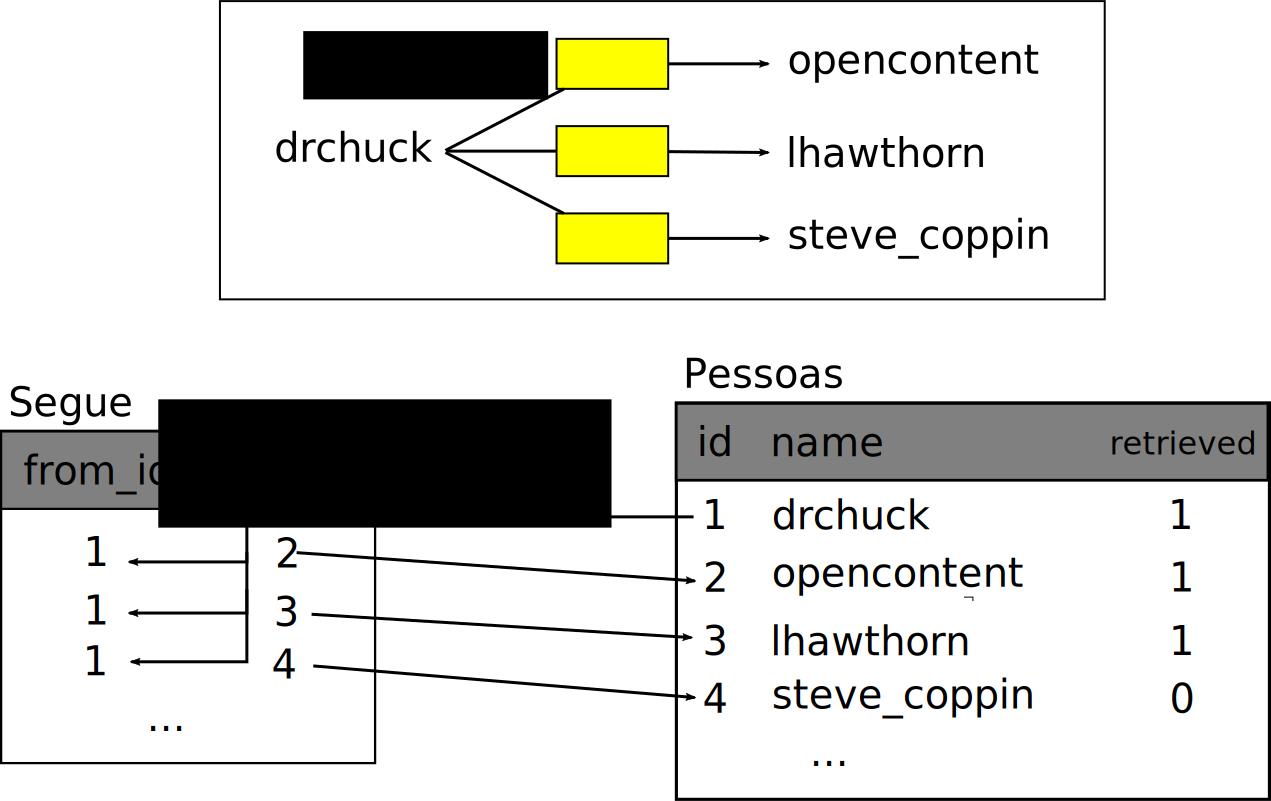
\includegraphics[height=2.50in]{figs2/twitter.eps}}
\afterfig


\section{Programming with multiple tables}

We will now redo the Twitter spider program using two tables, the primary
keys, and the key references as described above.  Here is the code for 
the new version of the program:

\beforeverb
\begin{verbatim}
import urllib
import twurl
import json
import sqlite3

TWITTER_URL = 'https://api.twitter.com/1.1/friends/list.json'

conn = sqlite3.connect('friends.sqlitesqlite3')
cur = conn.cursor()

cur.execute('''CREATE TABLE IF NOT EXISTS People 
    (id INTEGER PRIMARY KEY, name TEXT UNIQUE, retrieved INTEGER)''')
cur.execute('''CREATE TABLE IF NOT EXISTS Follows 
    (from_id INTEGER, to_id INTEGER, UNIQUE(from_id, to_id))''')

while True:
    acct = raw_input('Enter a Twitter account, or quit: ')
    if ( acct == 'quit' ) : break
    if ( len(acct) < 1 ) :
        cur.execute('''SELECT id, name FROM People 
            WHERE retrieved = 0 LIMIT 1''')
        try:
            (id, acct) = cur.fetchone()
        except:
            print 'No unretrieved Twitter accounts found'
            continue
    else:
        cur.execute('SELECT id FROM People WHERE name = ? LIMIT 1', 
            (acct, ) )
        try:
            id = cur.fetchone()[0]
        except:
            cur.execute('''INSERT OR IGNORE INTO People (name, retrieved) 
                VALUES ( ?, 0)''', ( acct, ) )
            conn.commit()
            if cur.rowcount != 1 : 
                print 'Error inserting account:',acct
                continue
            id = cur.lastrowid

    url = twurl.augment(TWITTER_URL, 
       {'screen_name': acct, 'count': '20'} )
    print 'Retrieving account', acct
    connection = urllib.urlopen(url)
    data = connection.read()
    headers = connection.info().dict
    print 'Remaining', headers['x-rate-limit-remaining']

    js = json.loads(data)
    # print json.dumps(js, indent=4)

    cur.execute('UPDATE People SET retrieved=1 WHERE name = ?', (acct, ) )

    countnew = 0
    countold = 0
    for u in js['users'] :
        friend = u['screen_name']
        print friend
        cur.execute('SELECT id FROM People WHERE name = ? LIMIT 1', 
            (friend, ) )
        try:
            friend_id = cur.fetchone()[0]
            countold = countold + 1
        except:
            cur.execute('''INSERT OR IGNORE INTO People (name, retrieved) 
                VALUES ( ?, 0)''', ( friend, ) )
            conn.commit()
            if cur.rowcount != 1 :
                print 'Error inserting account:',friend
                continue
            friend_id = cur.lastrowid
            countnew = countnew + 1
        cur.execute('''INSERT OR IGNORE INTO Follows (from_id, to_id) 
            VALUES (?, ?)''', (id, friend_id) )
    print 'New accounts=',countnew,' revisited=',countold
    conn.commit()

cur.close()
\end{verbatim}
\afterverb
%
This program is starting to get a bit complicated, but it illustrates
the patterns that we need to use when we are
using integer keys to link tables. The basic patterns are:

\begin{enumerate}

\item Create tables with primary keys and constraints.

\item When we have a logical key for a person (i.e., account
name) and we need the {\tt id} value for the person,
depending on whether or not the person is already
in the {\tt People} table we either need to: 
(1) look up the person in the {\tt People} table and 
retrieve the {\tt id} value for the person 
or (2) add the person to the {\tt People} table and get the 
{\tt id} value for the newly added row.

\item Insert the row that captures the ``follows'' relationship.

\end{enumerate}

We will cover each of these in turn.

\subsection{Constraints in database tables}

As we design our table structures, we can tell the database system 
that we would like it to enforce a few rules on us.   These rules
help us from making mistakes and introducing incorrect data into 
out tables.   When we create our tables:

\beforeverb
\begin{verbatim}
cur.execute('''CREATE TABLE IF NOT EXISTS People 
    (id INTEGER PRIMARY KEY, name TEXT UNIQUE, retrieved INTEGER)''')
cur.execute('''CREATE TABLE IF NOT EXISTS Follows 
    (from_id INTEGER, to_id INTEGER, UNIQUE(from_id, to_id))''')
\end{verbatim}
\afterverb
%
We indicate that the {\tt name} column in the {\tt People} table must be
{\tt UNIQUE}.   We also indicate that the combination of the two numbers
in each row of the {\tt Follows} table must be unique.  These constraints
keep us from making mistakes such as adding the same relationship more than
once.

We can take advantage of these constraints in the following code:

\beforeverb
\begin{verbatim}
cur.execute('''INSERT OR IGNORE INTO People (name, retrieved) 
    VALUES ( ?, 0)''', ( friend, ) )
\end{verbatim}
\afterverb
%
We add the {\tt OR IGNORE} clause to our {\tt INSERT} statement to indicate
that if this particular {\tt INSERT} would cause a violation of the
``{\tt name} must be unique'' rule, the database system is allowed to ignore the 
{\tt INSERT}.  We are using the database constraint as a safety net
to make sure we don't inadvertently do something incorrect.

Similarly, the following code ensures that we don't add the 
exact same {\tt Follows} relationship twice.

\beforeverb
\begin{verbatim}
cur.execute('''INSERT OR IGNORE INTO Follows 
    (from_id, to_id) VALUES (?, ?)''', (id, friend_id) )
\end{verbatim}
\afterverb
%
Again, we simply tell the database to ignore our attempted 
{\tt INSERT} if it would violate the uniqueness constraint
that we specified for the {\tt Follows} rows.

\subsection{Retrieve and/or insert a record}

When we prompt the user for a Twitter account, if the account 
exists, we must look up its {\tt id} value.  If the account
does not yet exist in the {\tt People} table, we must insert 
the record and get the {\tt id} value from the inserted
row.

This is a very common pattern and is done twice in the program above.
This code shows how we look up the {\tt id} for a 
friend's account when we have extracted a \verb"screen_name"
from a {\tt user} node in the retrieved Twitter JSON.

Since over time it will be increasingly likely that the account
will already be in the database, we first check to see if the
{\tt People} record exists using a {\tt SELECT} statement.

If all goes well\footnote{In general, when a sentence starts 
with ``if all goes well'' you will find that the code needs
to use try/except.} inside the {\tt try} section, we retrieve the
record using {\tt fetchone()} and then retrieve the
first (and only) element of the returned tuple and store it in 
\verb"friend_id".

If the {\tt SELECT} fails, the {\tt fetchone()[0]} code will fail
and control will transfer into the {\tt except} section.

\beforeverb
\begin{verbatim}
        friend = u['screen_name']
        cur.execute('SELECT id FROM People WHERE name = ? LIMIT 1',
            (friend, ) )
        try:
            friend_id = cur.fetchone()[0]
            countold = countold + 1
        except:
            cur.execute('''INSERT OR IGNORE INTO People (name, retrieved) 
                VALUES ( ?, 0)''', ( friend, ) )
            conn.commit()
            if cur.rowcount != 1 :
                print 'Error inserting account:',friend
                continue
            friend_id = cur.lastrowid
            countnew = countnew + 1
\end{verbatim}
\afterverb
%
If we end up in the {\tt except} code, it simply means that the row
was not found, so we must insert the row.  We use {\tt INSERT OR 
IGNORE} just to avoid errors and then call {\tt commit()} to 
force the database to really be updated.  After the write is done, we can 
check the {\tt cur.rowcount} to see how many rows were affected.  Since
we are attempting to insert a single row, if the number of 
affected rows is something other than 1, it is an error.  

If the {\tt INSERT} is successful, we can look at {\tt cur.lastrowid} 
to find out what value the database assigned to the {\tt id} column in 
our newly created row.

\subsection{Storing the friend relationship}

Once we know the key value for both the Twitter user
and the friend in the JSON, it is a simple matter to insert
the two numbers into the {\tt Follows} table
with the following code:

\beforeverb
\begin{verbatim}
cur.execute('INSERT OR IGNORE INTO Follows (from_id, to_id) VALUES (?, ?)',
    (id, friend_id) )
\end{verbatim}
\afterverb
%
Notice that we let the database take care of keeping us from ``double-inserting''
a relationship by creating the table with a uniqueness constraint and then
adding {\tt OR IGNORE} to our {\tt INSERT} statement.

Here is a sample execution of this program:

\beforeverb
\begin{verbatim}
Enter a Twitter account, or quit: 
No unretrieved Twitter accounts found
Enter a Twitter account, or quit: drchuck
Retrieving http://api.twitter.com/1.1/friends ...
New accounts= 20  revisited= 0
Enter a Twitter account, or quit: 
Retrieving http://api.twitter.com/1.1/friends ...
New accounts= 17  revisited= 3
Enter a Twitter account, or quit: 
Retrieving http://api.twitter.com/1.1/friends ...
New accounts= 17  revisited= 3
Enter a Twitter account, or quit: quit
\end{verbatim}
\afterverb
%
We started with the {\tt drchuck} account and then let the program
automatically pick the next two accounts to retrieve and add to 
our database.

The following is the first few rows in the {\tt People} 
and {\tt Follows} tables after this run is completed:

\beforeverb
\begin{verbatim}
People:
(1, u'drchuck', 1)
(2, u'opencontent', 1)
(3, u'lhawthorn', 1)
(4, u'steve_coppin', 0)
(5, u'davidkocher', 0)
55 rows.
Follows:
(1, 2)
(1, 3)
(1, 4)
(1, 5)
(1, 6)
60 rows.
\end{verbatim}
\afterverb
%
You can see the {\tt id}, {\tt name}, and {\tt visited} fields in the 
{\tt People} table and you see the numbers of both ends of 
the relationship in the {\tt Follows} table.   
In the {\tt People} table, we can see that the first three people
have been visited and their data has been retrieved.
The data in the {\tt Follows} table indicates that
{\tt drchuck} (user 1) is a friend to all of the people shown in the first
five rows.  This makes sense because
the first data we retrieved and stored was the Twitter friends of
{\tt drchuck}.  If you were to print more rows from the {\tt Follows} table,
you would see the friends of users 2 and 3 as well.

\section{Three kinds of keys}

Now that we have started building a data model putting our
data into multiple linked tables and linking the rows in those
tables using {\bf keys}, we need to look at some terminology 
around keys.  There are generally three kinds of keys used 
in a database model.

\begin{itemize}

\item A {\bf logical key} is a key that the ``real world'' might use
to look up a row.   In our example data model, the {\tt name}
field is a logical key.  It is the screen name for the user 
and we indeed look up a user's row several times in the program
using the {\tt name} field.  You will often find that it makes
sense to add a {\tt UNIQUE} constraint to a logical key.  Since the 
logical key is how we look up a row from the outside world, it makes
little sense to allow multiple rows with the same value in the table.

\item A {\bf primary key} is usually a number that is assigned
automatically by the database.  It generally has no meaning outside
the program and is only used to link rows from different tables
together.  When we want to look up a row in a table, usually 
searching for the row using the primary key is the fastest 
way to find the row.  Since primary keys are integer numbers, they 
take up very little storage and can be compared or sorted very quickly.
In our data model, the {\tt id} field is an example of a primary key.

\item A {\bf foreign key} is usually a number that points to the primary key
of an associated row in a different table.  An example of a foreign
key in our data model is the \verb"from_id".  

\end{itemize}

We are using a
naming convention of always calling the primary key field name
{\tt id} and appending the suffix \verb"_id" to any field name
that is a foreign key.


\section{Using JOIN to retrieve data}

Now that we have followed the rules of database normalization
and have data separated into two tables, linked together using
primary and foreign keys, we need to be able to build a 
{\tt SELECT} that reassembles the data across the tables.

SQL uses the {\tt JOIN} clause to reconnect these tables.  
In the {\tt JOIN} clause you specify the fields that are used 
to reconnect the rows between the tables.

The following is an example of a {\tt SELECT} with a 
{\tt JOIN} clause:

\beforeverb
\begin{verbatim}
SELECT * FROM Follows JOIN People 
    ON Follows.from_id = People.id WHERE People.id = 1
\end{verbatim}
\afterverb
%
The {\tt JOIN} clause indicates that the fields we are selecting
cross both the {\tt Follows} and {\tt People} tables.  The {\tt ON}
clause indicates how the two tables are to be joined:  Take the rows
from {\tt Follows} and append the row from {\tt People} where the
field \verb"from_id" in {\tt Follows} is the same the {\tt id} value
in the {\tt People} table.

\beforefig
\centerline{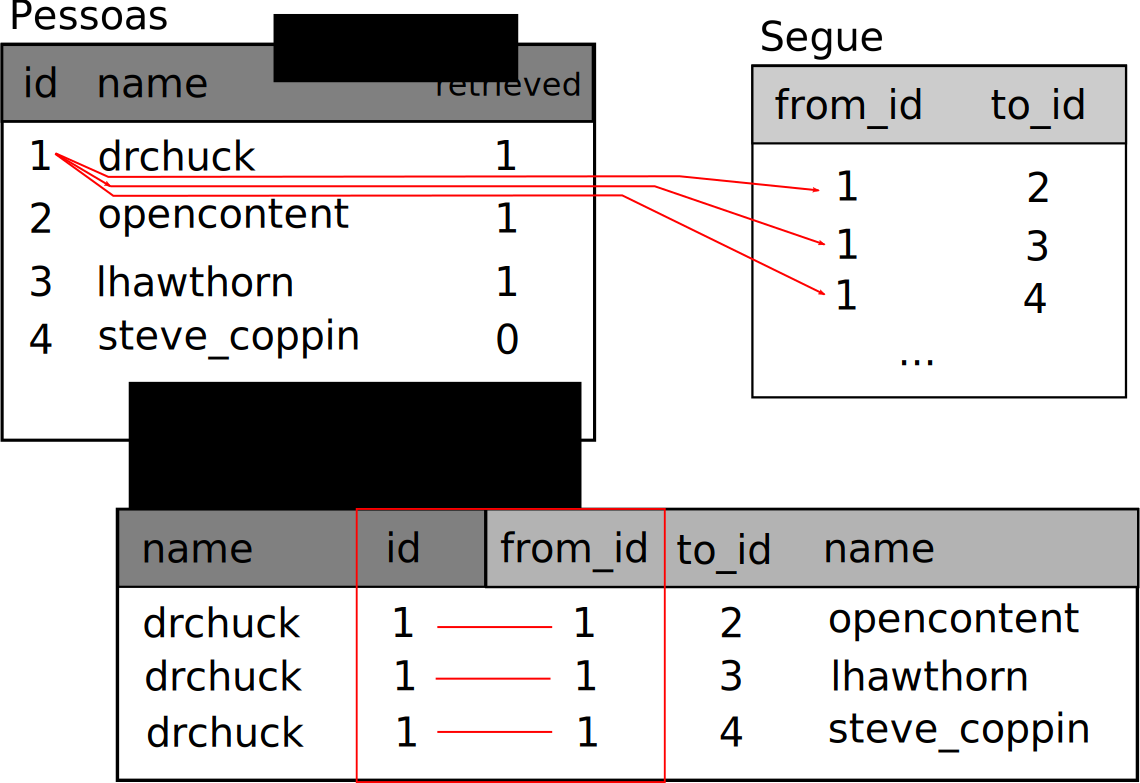
\includegraphics[height=2.50in]{figs2/join.eps}}
\afterfig

The result of the JOIN is to create extra-long ``metarows'' which have both 
the fields from {\tt People} and the matching fields from {\tt Follows}.
Where there is more than one match between the {\tt id} field from {\tt People}
and the \verb"from_id" from {\tt People}, then JOIN creates a metarow 
for \emph{each} of the matching pairs of rows, duplicating data as needed.

The following code demonstrates the data that we will have in the 
database after the multi-table Twitter spider program (above) has
been run several times.

\beforeverb
\begin{verbatim}
import sqlite3

conn = sqlite3.connect('spider.sqlite3')
cur = conn.cursor()

cur.execute('SELECT * FROM People')
count = 0
print 'People:'
for row in cur :
   if count < 5: print row
   count = count + 1
print count, 'rows.'

cur.execute('SELECT * FROM Follows')
count = 0
print 'Follows:'
for row in cur :
   if count < 5: print row
   count = count + 1
print count, 'rows.'

cur.execute('''SELECT * FROM Follows JOIN People 
    ON Follows.to_id = People.id WHERE Follows.from_id = 2''')
count = 0
print 'Connections for id=2:'
for row in cur :
   if count < 5: print row
   count = count + 1
print count, 'rows.'

cur.close()
\end{verbatim}
\afterverb
%
In this program, we first dump out the {\tt People}
and {\tt Follows} and then dump out a subset of the
data in the tables joined together.

Here is the output of the program:

\beforeverb
\begin{verbatim}
python twjoin.py 
People:
(1, u'drchuck', 1)
(2, u'opencontent', 1)
(3, u'lhawthorn', 1)
(4, u'steve_coppin', 0)
(5, u'davidkocher', 0)
55 rows.
Follows:
(1, 2)
(1, 3)
(1, 4)
(1, 5)
(1, 6)
60 rows.
Connections for id=2:
(2, 1, 1, u'drchuck', 1)
(2, 28, 28, u'cnxorg', 0)
(2, 30, 30, u'kthanos', 0)
(2, 102, 102, u'SomethingGirl', 0)
(2, 103, 103, u'ja_Pac', 0)
20 rows.
\end{verbatim}
\afterverb
%
You see the columns from the {\tt People} and {\tt Follows} tables and the last
set of rows is the result of the {\tt SELECT} with the {\tt JOIN} clause.

In the last select, we are looking for accounts that are friends of 
``opencontent'' (i.e., {\tt People.id=2}).

In each of the ``metarows'' in the last select, the first two columns are
from the {\tt Follows}
table followed by columns three through five from the {\tt People} table.  You can also
see that the second column (\verb"Follows.to_id") matches the third column
({\tt People.id}) in each of the joined-up ``metarows''.

\section{Summary}

This chapter has covered a lot of ground to give you an overview of the basics
of using a database in Python.   It is more complicated to write the code to use 
a database to store data than Python dictionaries or flat files so there is 
little reason to use a database unless your application truly needs the capabilities
of a database.  The situations where a database can be quite useful are: 
(1) when your application needs to make small many random updates within a large data set,
(2) when your data is so large it cannot fit in a dictionary and you need to 
look up information repeatedly, or (3) when you have a long-running process that you
want to be able to stop and restart and retain the data from one run to the next.

You can build a simple database with a single table to suit many application 
needs, but most problems will require several tables and links/relationships
between rows in different tables.   When you start making links between 
tables, it is important to do some thoughtful design and follow the 
rules of database normalization to make the best use of the database's
capabilities.  Since the primary motivation for using a database
is that you have a large amount of data to deal with, it is important
to model your data efficiently so your programs run as fast as possible.

\section{Debugging}

One common pattern when you are developing a Python program to connect to
an SQLite database will be to run a Python program and check the
results using the SQLite Database Browser.  The browser allows you 
to quickly check to see if your program is working properly.

You must be careful because SQLite takes care to keep two programs
from changing the same data at the same time.   For example, if
you open a database in the browser and make a change to the database
and have not yet pressed the ``save'' button in the browser, the 
browser ``locks'' the database file and keeps any other program
from accessing the file.  In particular, your Python program
will not be able to access the file if it is locked.

So a solution is to make sure to either close the database browser 
or use the {\bf File} menu to close the database in the browser
before you attempt to access the database from Python to avoid
the problem of your Python code failing because the database is
locked.

\section{Glossary}

\begin{description}

\item[attribute:] One of the values within a tuple.  More commonly
called a ``column'' or ``field''.
\index{attribute}

\item[constraint:] 
When we tell the database to enforce a rule on a field or a row
in a table.  A common constraint is to insist that there can be no
duplicate values in a particular field (i.e., all the values must be unique).
\index{constraint}

\item[cursor:] A cursor allows you to execute SQL commands in a database
and retrieve data from the database.  A cursor is similar to 
a socket or file handle for network connections and files, respectively.
\index{cursor}

\item[database browser:] 
A piece of software that allows you to directly connect to a database 
and manipulate the database directly without writing a program.
\index{database browser}

\item[foreign key:] A numeric key that points to the primary key of 
a row in another table.  Foreign keys establish relationships between rows
stored in different tables.
\index{foreign key}

\item[index:] Additional data that the database software maintains as rows
and inserts into a table to make lookups very fast.
\index{index}

\item[logical key:] A key that the ``outside world'' uses to look up a particular
row.  For example in a table of user accounts, a person's email address
might be a good candidate as the logical key for the user's data. 
\index{logical key}

\item[normalization:] Designing a data model so that no data
is replicated.  We store each item of data at one place in the database
and reference it elsewhere using a foreign key.
\index{normalization}
\index{database normalization}

\item[primary key:] A numeric key assigned to each row that is used to 
refer to one row in a table from another table.  Often the database
is configured to automatically assign primary keys as rows are inserted.
\index{primary key}

\item[relation:] An area within a database that contains tuples and 
attributes.  More typically called a ``table''.
\index{relation}

\item[tuple:] A single entry in a database table that is a set 
of attributes.  More typically called ``row''.
\index{tuple}

\end{description}


% TODO % The contents of this file is 
% Copyright (c) 2009-  Charles R. Severance, All Righs Reserved

\chapter{Visualizando dados}
%\chapter{Visualizing data}

Até agora, nós aprendemos a linguagem Python, como utilizá-la,
para trabalhar com redes e banco de dados para manipular dados.
%So far we have been learning the Python language and then 
%learning how to use Python, the network, and databases 
%to manipulate data.

Neste capítulo, serão apresentadas três aplicações completas
que utilizarão todos estes conceitos para gerenciar e visualizar
dados. Você pode utilizar estas aplicações como exemplo de código
que podem ajudar na solução de problemas reais. 
%In this chapter, we take a look at three 
%complete applications that bring all of these things together
%to manage and visualize data.  You  might use these applications 
%as sample code to help get you started in solving a
%real-world problem.

Cada uma das aplicações é um arquivo ZIP que você pode fazer
download, extrair para o seu computador e executar.
%Each of the applications is a ZIP file that you can download
%and extract onto your computer and execute.

\section{Construindo um mapa no Google a partir de dados geocodificados}
\index{Google!map}
\index{Visualização!mapas}
%\section{Building a Google map from geocoded data}
%\index{Google!map}
%\index{Visualization!map}

Neste projeto, nós utilizaremos a API de geocodificação do
Google para obter algumas localizações geográficas informadas
pelos usuários de nomes de universidades e colocar os dados
em um mapa no Google.
%In this project, we are using the Google geocoding API
%to clean up some user-entered geographic locations of 
%university names and then placing the data on a Google
%map.  

\beforefig
\centerline{\includegraphics[height=2.25in]{figs2/google-map.eps}}
\afterfig
%\beforefig
%\centerline{\includegraphics[height=2.25in]{figs2/google-map.eps}}
%\afterfig

Para iniciar, faça o download da aplicação em:
%To get started, download the application from:

\url{www.py4inf.com/code/geodata.zip}

O primeiro problema a ser resolvido é que a API gratuita de 
geocodificação do Google limita o número de requisições por dia.
Se você tiver muitos dados, você pode precisar parar e reiniciar
o processo de busca muitas vezes. Nós podemos quebrar o problema
em duas fases.
%The first problem to solve is that the free Google geocoding
%API is rate-limited to a certain number of requests per day.  If you have
%a lot of data, you might need to stop and restart the lookup
%process several times.  So we break the problem into two
%phases.  

\index{cache}
Na primeira fase nós faremos uma ``'pesquisa'' nos dados do arquivo
{\bf where.data} e então ler uma linha por vez, retornando a informação
geocodificada do Google e armazenar em um banco de dados {\bf geodata.sqlite}.
Antes de efetuar a pesquisa no Google, utilizando a API, para cada localização
informada pelo usuário, nós vamos checar para ver se já existe este dado
para a localização informada. O banco de dados está funcionando como um
``cache'' local dos nossos dados de localização para ter certeza que nunca
buscaremos no Google duas vezes pelo mesmo dado.
%\index{cache}
%In the first phase we take our input ``survey'' data in the file
%{\bf where.data} and read it one line at a time, and retrieve the
%geocoded information from Google and store it 
%in a database {\bf geodata.sqlite}.
%Before we use the geocoding API for each user-entered location, 
%we simply check to see if we already have the data for that 
%particular line of input.  The database is functioning as a 
%local ``cache'' of our geocoding data to make sure we never ask 
%Google for the same data twice.

Você pode reiniciar o processo a qualquer hora deletando o arquivo 
{\bf geodata.sqlite}.
%You can restart the process at any time by removing the file
%{\bf geodata.sqlite}.

Execute o programa {\bf geoload.py}. Este programa fará a leitura das linhas
do arquivo {\bf where.data} e para cada linha checar se o dado já existe no
banco de dados. Se nós não tivermos o dado para a localização, será utilizada
a API para retornar o dado e armazená-lo no banco de dados.  
%Run the {\bf geoload.py} program.   This program will read the input
%lines in {\bf where.data} and for each line check to see if it is already
%in the database.  If we don't have the data for the location, it will
%call the geocoding API to retrieve the data and store it in 
%the database.

Aqui está uma simples execução após a coleta de alguns dados no
banco de dados:
%Here is a sample run after there is already some data in the 
%database:

\beforeverb
\begin{verbatim}
Found in database  Northeastern University
Found in database  University of Hong Kong, ...
Found in database  Technion
Found in database  Viswakarma Institute, Pune, India
Found in database  UMD
Found in database  Tufts University

Resolving Monash University
Retrieving http://maps.googleapis.com/maps/api/
    geocode/json?sensor=false&address=Monash+University
Retrieved 2063 characters {    "results" : [  
{u'status': u'OK', u'results': ... }

Resolving Kokshetau Institute of Economics and Management
Retrieving http://maps.googleapis.com/maps/api/
    geocode/json?sensor=false&address=Kokshetau+Inst ...
Retrieved 1749 characters {    "results" : [  
{u'status': u'OK', u'results': ... }
...
\end{verbatim}
\afterverb
%

As primeiras cinco execuções já estão no banco de dados e então serão
ignoradas. O programa encontra o ponto onde parou e então continua
o trabalho recuperando novas informações.
%The first five locations are already in the database and so they 
%are skipped.  The program scans to the point where it finds new
%locations and starts retrieving them.

O programa {\bf geoload.py} pode ser parado a qualquer hora, e há um
contador que você pode utilizar para limitar o número de chamadas para a
API de geocodificação a cada execução. Dado o arquivo {\bf where.data}, que
possui algumas centenas de itens, você não consegue ultrapassar o limite diário,
mas pode fazer várias execuções em vários dias diferentes para ir pegando
aos poucos todos os dados que você precisa.
%The {\bf geoload.py} program can be stopped at any time, and there is a counter 
%that you can use to limit the number of calls to the geocoding
%API for each run.  Given that the {\bf where.data} only has a few hundred
%data items, you should not run into the daily rate limit, but if you 
%had more data it might take several runs over several days to 
%get your database to have all of the geocoded data for your input.

Uma vez que você tiver alguns dados carregados em {\bf geodata.sqlite},
você pode visualizar os dados utilizando o programa {\bf geodump.py}.
Este programa lê o banco de dados e escreve no arquivo {\bf where.js}
com a localização de latitude e longitude em um formato de código 
JavaScript.
%Once you have some data loaded into {\bf geodata.sqlite}, you can 
%visualize the data using the {\bf geodump.py} program.  This
%program reads the database and writes the file {\bf where.js}
%with the location, latitude, and longitude in the form of
%executable JavaScript code.   

Segue uma execução do programa {\bf geodump.py}:
%A run of the {\bf geodump.py} program is as follows:

\beforeverb
\begin{verbatim}
Northeastern University, ... Boston, MA 02115, USA 42.3396998 -71.08975
Bradley University, 1501 ... Peoria, IL 61625, USA 40.6963857 -89.6160811
...
Technion, Viazman 87, Kesalsaba, 32000, Israel 32.7775 35.0216667
Monash University Clayton ... VIC 3800, Australia -37.9152113 145.134682
Kokshetau, Kazakhstan 53.2833333 69.3833333
...
12 records written to where.js
Open where.html to view the data in a browser
\end{verbatim}
\afterverb
%

O arquivo {\bf where.html} consiste de um HTML e um JavaScript para visualizar
um mapa Google. Ele lê os dados mais recentes em {\bf where.js} para pegar
os dados a serem visualizados. Aqui está um formato do arquivo {\bf where.js}.
%The file {\bf where.html} consists of HTML and JavaScript to visualize 
%a Google map.  It reads the most recent data in {\bf where.js} to get 
%the data to be visualized.  Here is the format of the {\bf where.js} file:

\beforeverb
\begin{verbatim}
myData = [
[42.3396998,-71.08975, 'Northeastern Uni ... Boston, MA 02115'],
[40.6963857,-89.6160811, 'Bradley University, ... Peoria, IL 61625, USA'],
[32.7775,35.0216667, 'Technion, Viazman 87, Kesalsaba, 32000, Israel'],
   ...
];
\end{verbatim}
\afterverb
%

Esta é uma variável JavaScript que contém uma lista de listas.
A sintaxe para representação de listas em JavaScript é muito similar
ao Python, sendo assim, deve ser familiar para você também.
%This is a JavaScript variable that contains a list of lists.  
%The syntax for JavaScript list constants is very similar to 
%Python, so the syntax should be familiar to you.

Simplemente abra o arquivo {\bf where.html} em um browser para ver as
localizações. Você pode passar o mouse por cima de cada um dos pontos 
do mapa para encontrar a localização que a API de geocodificação retornou
para uma entrada do usuário. Se você não puder ver qualquer dado quando
abrir o arquivo {\bf where.html}, você pode querer checar o console do
desenvolvedor (JavaScript) de seu browser e ver se envcontra algum erro.
%Simply open {\bf where.html} in a browser to see the locations.  You 
%can hover over each map pin to find the location that the 
%geocoding API returned for the user-entered input.  If you 
%cannot see any data when you open the {\bf where.html} file, you might 
%want to check the JavaScript or developer console for your browser.

\section{Visualizando redes e interconexões}
\index{Google!page rank}
\index{Visualização!redes}
\index{Visualização!page rank}
%\section{Visualizing networks and interconnections}
%\index{Google!page rank}
%\index{Visualization!networks}
%\index{Visualization!page rank}

Nesta aplicação, vamos realizar algumas das funções de um motor de busca.
Nós primeiramente vamos extrair um pequeno pedaço da web e rodar
uma versão simplificada do algoritmo de page rank do Google para determinar
quais páginas estão altamente conectadas, e então visualizar o page rank
e a conectividade de nosso pequeno pedaço da web.
Utilizaremos a biblioteca de visualização JavaScript D3 \url{http://d3js.org/}
para produzir a saída da visualização.
%In this application, we will perform some of the functions of a search
%engine.   We will first spider a small subset of the web and run
%a simplified version of the Google page rank algorithm to
%determine which pages are most highly connected, and then visualize
%the page rank and connectivity of our small corner of the web.
%We will use the D3 JavaScript visualization library 
%\url{http://d3js.org/} to produce the visualization output.

Você pode fazer download e extrair esta aplicação de:
%You can download and extract this application from:

\url{www.py4inf.com/code/pagerank.zip}

\beforefig
\centerline{\includegraphics[height=2.25in]{figs2/pagerank.eps}}
\afterfig

O primeiro programa ({\bf spider.py}) vasculha páginas web e grava
uma série de páginas no banco de dados ({\bf spider.sqlite}), gravando
as ligações entre as páginas. Você pode reiniciar o processo a qualquer
hora deletando o arquivo {\bf spider.sqlite} e reexecutando o {\bf spider.py}.
%The first program ({\bf spider.py}) program crawls a web 
%site and pulls a series of pages into the
%database ({\bf spider.sqlite}), recording the links between pages.
%You can restart the process at any time by removing the 
%{\bf spider.sqlite} file and rerunning {\bf spider.py}.

\beforeverb
\begin{verbatim}
Enter web url or enter: http://www.dr-chuck.com/
['http://www.dr-chuck.com']
How many pages:2
1 http://www.dr-chuck.com/ 12
2 http://www.dr-chuck.com/csev-blog/ 57
How many pages:
\end{verbatim}
\afterverb
%

Neste exemplo de execução, nós pedimos ao programa para extrair e 
retornar duas páginas. Se você reiniciar o programa e pedir a ele para
obter mais páginas, não irá pegar novamente as mesmas páginas que já
estão no banco de dados. Após o restart ele vai sortear randomicamente
páginas e começar de lá. Assim, cada execução sucessiva do {\bf spider.py}
é um aditivo.
%In this sample run, we told it to crawl a website and retrieve two 
%pages.  If you restart the program and tell it to crawl more
%pages, it will not re-crawl any pages already in the database.  Upon 
%restart it goes to a random non-crawled page and starts there.  So 
%each successive run of {\bf spider.py} is additive.

\beforeverb
\begin{verbatim}
Enter web url or enter: http://www.dr-chuck.com/
['http://www.dr-chuck.com']
How many pages:3
3 http://www.dr-chuck.com/csev-blog 57
4 http://www.dr-chuck.com/dr-chuck/resume/speaking.htm 1
5 http://www.dr-chuck.com/dr-chuck/resume/index.htm 13
How many pages:
\end{verbatim}
\afterverb
%

Você pode ter múltiplos pontos de start no mesmo banco de dados, dentro
do programa, eles são chamados ``webs''. O programa escolhe randomicamente
um dos links que ainda não foi visitado através de toda a web como sendo
a próxima página a ser visitada.
%You can have multiple starting points in the same database---within
%the program, these are called ``webs''.   The spider
%chooses randomly amongst all non-visited links across all
%the webs as the next page to spider.

Se você quer visualizar o conteúdo do arquivo {\bf spider.sqlite}, você pode
rodar o programa {\bf spdump.py}, como segue:
%If you want to dump the contents of the {\bf spider.sqlite} file, you can 
%run {\bf spdump.py} as follows:

\beforeverb
\begin{verbatim}
(5, None, 1.0, 3, u'http://www.dr-chuck.com/csev-blog')
(3, None, 1.0, 4, u'http://www.dr-chuck.com/dr-chuck/resume/speaking.htm')
(1, None, 1.0, 2, u'http://www.dr-chuck.com/csev-blog/')
(1, None, 1.0, 5, u'http://www.dr-chuck.com/dr-chuck/resume/index.htm')
4 rows.
\end{verbatim}
\afterverb
%

Isto mostra o número de links visitados, o antigo page rank, o novo page
rank, o id da página, e a url da página. O programa {\bf spdump.py} somente
mostra páginas que tem pelo menos um link já visitado.
%This shows the number of incoming links, the old page rank, the new page
%rank, the id of the page, and the url of the page.  The {\bf spdump.py} program
%only shows pages that have at least one incoming link to them.

Uma vez que você tem algumas páginas no banco de dados, você pode rodar o page 
rank nas páginas usando o programa {\bf sprank.py}. Você apenas diz quantas
iterações de páginas devem ser executadas.
%Once you have a few pages in the database, you can run page rank on the
%pages using the {\bf sprank.py} program.  You simply tell it how many page
%rank iterations to run.

\beforeverb
\begin{verbatim}
How many iterations:2
1 0.546848992536
2 0.226714939664
[(1, 0.559), (2, 0.659), (3, 0.985), (4, 2.135), (5, 0.659)]
\end{verbatim}
\afterverb
%
Você pode analisar o banco de dados novamente para ver se o page rank foi
atualizado:
%You can dump the database again to see that page rank has been updated:

\beforeverb
\begin{verbatim}
(5, 1.0, 0.985, 3, u'http://www.dr-chuck.com/csev-blog')
(3, 1.0, 2.135, 4, u'http://www.dr-chuck.com/dr-chuck/resume/speaking.htm')
(1, 1.0, 0.659, 2, u'http://www.dr-chuck.com/csev-blog/')
(1, 1.0, 0.659, 5, u'http://www.dr-chuck.com/dr-chuck/resume/index.htm')
4 rows.
\end{verbatim}
\afterverb
%

Você pode rodar o {\bf sprank.py} quantas vezes quiser, isto irá apenas refinar
o page rank cada vez que você executar. Pode até mesmo rodar o {\bf sprank.py} um
pequeno número de vezes e então recuperar mais algumas páginas com o {\bf spider.py} 
e então rodar o {\bf sprank.py} para recuperar os valores do page rank. Um motor de
pesquisa geralmente roda os programas de recuperação e rankeamento ao mesmo tempo.
%You can run {\bf sprank.py} as many times as you like and it will simply refine
%the page rank each time you run it.  You can even run {\bf sprank.py} a few times
%and then go spider a few more pages sith {\bf spider.py} and then run {\bf sprank.py}
%to reconverge the page rank values.  A search engine usually runs both the crawling and 
%ranking programs all the time.

Se você quiser reiniciar os cálculos de page rank sem fazer a extração das páginas
web novamente, você pode usar o {\bf spreset.py} e então reiniciar o {\bf sprank.py}.
%If you want to restart the page rank calculations without respidering the 
%web pages, you can use {\bf spreset.py} and then restart {\bf sprank.py}.

\beforeverb
\begin{verbatim}
How many iterations:50
1 0.546848992536
2 0.226714939664
3 0.0659516187242
4 0.0244199333
5 0.0102096489546
6 0.00610244329379
...
42 0.000109076928206
43 9.91987599002e-05
44 9.02151706798e-05
45 8.20451504471e-05
46 7.46150183837e-05
47 6.7857770908e-05
48 6.17124694224e-05
49 5.61236959327e-05
50 5.10410499467e-05
[(512, 0.0296), (1, 12.79), (2, 28.93), (3, 6.808), (4, 13.46)]
\end{verbatim}
\afterverb
%

Para cada iteração do algoritmo de page rank, ele imprime a média
de modificações no page rank por página. A rede inicia-se
desbalanceada e então os valores do page rank individual mudam
com velocidade entre as iterações. Mas em poucas iterações, o page rank 
coverge. Você deve rodar o {\bf prank.py} por tempo suficiente para
que os valores de page rank possam convergir.
%For each iteration of the page rank algorithm it prints the average
%change in page rank per page.   The network initially is quite
%unbalanced and so the individual page rank values change wildly between
%iterations. But in a few short iterations, the page rank converges.  You
%should run {\bf prank.py} long enough that the page rank values converge.

Se você quer visualizar as primeiras páginas no rank, rode o {\bf spjson.py}
para ler o banco de dados e escrever os dados dos links com maior pontuação
no formato JSON para serem vistos no web browser.
%If you want to visualize the current top pages in terms of page rank,
%run {\bf spjson.py} to read the database and write the data for the 
%most highly linked pages in JSON format to be viewed in a
%web browser.

\beforeverb
\begin{verbatim}
Creating JSON output on spider.json...
How many nodes? 30
Open force.html in a browser to view the visualization
\end{verbatim}
\afterverb
%\beforeverb
%\begin{verbatim}
%Creating JSON output on spider.json...
%How many nodes? 30
%Open force.html in a browser to view the visualization
%\end{verbatim}
%\afterverb
%

Você pode visualizar este dado abrindo o arquivo {\bf force.html} em seu web 
browser. Isto mostra um layout automático de nós e links. Você pode clicar e
arrastar qualquer nó e também dar um duplo clique no nó para encontrar a URL
que ele representa.
%You can view this data by opening the file {\bf force.html} in your web browser.  
%This shows an automatic layout of the nodes and links.  You can click and 
%drag any node and you can also double-click on a node to find the URL
%that is represented by the node.

Se você rodar novamente
%If you rerun the other utilities, rerun {\bf spjson.py} and
%press refresh in the browser to get the new data from {\bf spider.json}.

\section{Visualizing mail data}

Up to this point in the book, you have become quite familiar with our 
{\bf mbox-short.txt} and {\bf mbox.txt} data files.   Now it is time to take
our analysis of email data to the next level.  

In the real world, sometimes you have to pull down mail data from servers.
That might take quite some time and the data might be inconsistent, 
error-filled, and need a lot of cleanup or adjustment.  In this section, we
work with an application that is the most complex so far and pull down nearly a 
gigabyte of data and visualize it.

\beforefig
\centerline{\includegraphics[height=2.50in]{figs2/wordcloud.eps}}
\afterfig

You can download this application from:

\url{www.py4inf.com/code/gmane.zip}

We will be using data from a free email list archiving service called 
\url{www.gmane.org}.  This service is very popular with open source
projects because it provides a nice searchable archive of their 
email activity.  They also have a very liberal policy regarding accessing 
their data through their API.  They have no rate limits, but ask that you 
don't overload their service and take only the data you need.  You can read
gmane's terms and conditions at this page:

\url{http://gmane.org/export.php}

{\em It is very important that you make use of the gmane.org data
responsibly by adding delays to your access of their services and spreading
long-running jobs over a longer period of time.  Do not abuse this free service
and ruin it for the rest of us.}

When the Sakai email data was spidered using this software, it produced nearly 
a Gigabyte of data and took a number of runs on several days.
The file {\bf README.txt} in the above ZIP may have instructions as to how
you can download a pre-spidered copy of the {\bf content.sqlite} file for 
a majority of the Sakai email corpus so you don't have to spider for 
five days just to run the programs.  If you download the pre-spidered
content, you should still run the spidering process to catch up with 
more recent messages.

The first step is to spider the gmane repository.  The base URL 
is hard-coded in the {\bf gmane.py} and is hard-coded to the Sakai
developer list.  You can spider another repository by changing that
base url.   Make sure to delete the {\bf content.sqlite} file if you 
switch the base url.  

The {\bf gmane.py} file operates as a responsible caching spider in 
that it runs slowly and retrieves one mail message per second so 
as to avoid getting throttled by gmane.   It stores all of
its data in a database and can be interrupted and restarted 
as often as needed.   It may take many hours to pull all the data
down.  So you may need to restart several times.

Here is a run of {\bf gmane.py} retrieving the last five messages of the
Sakai developer list:

\beforeverb
\begin{verbatim}
How many messages:10
http://download.gmane.org/gmane.comp.cms.sakai.devel/51410/51411 9460
    nealcaidin@sakaifoundation.org 2013-04-05 re: [building ...
http://download.gmane.org/gmane.comp.cms.sakai.devel/51411/51412 3379
    samuelgutierrezjimenez@gmail.com 2013-04-06 re: [building ...
http://download.gmane.org/gmane.comp.cms.sakai.devel/51412/51413 9903
    da1@vt.edu 2013-04-05 [building sakai] melete 2.9 oracle ...
http://download.gmane.org/gmane.comp.cms.sakai.devel/51413/51414 349265
    m.shedid@elraed-it.com 2013-04-07 [building sakai] ...
http://download.gmane.org/gmane.comp.cms.sakai.devel/51414/51415 3481
    samuelgutierrezjimenez@gmail.com 2013-04-07 re: ...
http://download.gmane.org/gmane.comp.cms.sakai.devel/51415/51416 0

Does not start with From 
\end{verbatim}
\afterverb
%
The program scans {\bf content.sqlite} from one up to the first message number not
already spidered and starts spidering at that message.  It continues spidering
until it has spidered the desired number of messages or it reaches a page
that does not appear to be a properly formatted message.

Sometimes \url{gmane.org} is missing a message.  Perhaps administrators can delete messages
or perhaps they get lost.   If your spider stops, and it seems it has hit
a missing message, go into the SQLite Manager and add a row with the missing id leaving
all the other fields blank and restart {\bf gmane.py}.   This will unstick the 
spidering process and allow it to continue.  These empty messages will be ignored in the next
phase of the process.

One nice thing is that once you have spidered all of the messages and have them in 
{\bf content.sqlite}, you can run {\bf gmane.py} again to get new messages as 
they are sent to the list.  

The {\bf content.sqlite} data is pretty raw, with an inefficient data model, 
and not compressed.
This is intentional as it allows you to look at {\bf content.sqlite}
in the SQLite Manager to debug problems with the spidering process.
It would be a bad idea to run any queries against this database, as they 
would be quite slow.

The second process is to run the program {\bf gmodel.py}.  This program reads the raw 
data from {\bf content.sqlite} and produces a cleaned-up and well-modeled version of the 
data in the file {\bf index.sqlite}.  This file will be much smaller (often 10X
smaller) than {\bf content.sqlite} because it also compresses the header and body text.

Each time {\bf gmodel.py} runs it deletes and rebuilds {\bf index.sqlite}, allowing
you to adjust its parameters and edit the mapping tables in {\bf content.sqlite} to tweak the 
data cleaning process. This is a sample run of {\bf gmodel.py}.  It prints a line out each time
250 mail messages are processed so you can see some progress happening, as this program may
run for a while processing nearly a Gigabyte of mail data.

\beforeverb
\begin{verbatim}
Loaded allsenders 1588 and mapping 28 dns mapping 1
1 2005-12-08T23:34:30-06:00 ggolden22@mac.com
251 2005-12-22T10:03:20-08:00 tpamsler@ucdavis.edu
501 2006-01-12T11:17:34-05:00 lance@indiana.edu
751 2006-01-24T11:13:28-08:00 vrajgopalan@ucmerced.edu
...
\end{verbatim}
\afterverb
%

The {\bf gmodel.py} program handles a number of data cleaning tasks.

Domain names are truncated to two levels for .com, .org, .edu, and .net.
Other domain names are truncated to three levels.  So si.umich.edu becomes
umich.edu and caret.cam.ac.uk becomes cam.ac.uk.   Email addresses are also
forced to lower case, and some of the @gmane.org address like the following

\beforeverb
\begin{verbatim}
   arwhyte-63aXycvo3TyHXe+LvDLADg@public.gmane.org
\end{verbatim}
\afterverb
%
are converted to the real address whenever there is a matching real email
address elsewhere in the message corpus.

In the {\bf content.sqlite} database there are two tables that allow
you to map both domain names and individual email addresses that change over 
the lifetime of the email list.  For example, Steve Githens used the following
email addresses as he changed jobs over the life of the Sakai developer list:

\beforeverb
\begin{verbatim}
s-githens@northwestern.edu
sgithens@cam.ac.uk
swgithen@mtu.edu
\end{verbatim}
\afterverb
%
We can add two entries to the Mapping table in {\bf content.sqlite} so 
{\bf gmodel.py} will map all three to one address:

\beforeverb
\begin{verbatim}
s-githens@northwestern.edu ->  swgithen@mtu.edu
sgithens@cam.ac.uk -> swgithen@mtu.edu
\end{verbatim}
\afterverb
%
You can also make similar entries in the DNSMapping table if there are multiple
DNS names you want mapped to a single DNS.  The following mapping was added to the Sakai data:

\beforeverb
\begin{verbatim}
iupui.edu -> indiana.edu
\end{verbatim}
\afterverb
%
so all the accounts from the various Indiana University campuses are tracked together.

You can rerun the {\bf gmodel.py} over and over as you look at the data, and add mappings
to make the data cleaner and cleaner.   When you are done, you will have a nicely
indexed version of the email in {\bf index.sqlite}.   This is the file to use to do data
analysis.   With this file, data analysis will be really quick.

The first, simplest data analysis is to determine "who sent the most mail?" and "which 
organization sent the most mail"?  This is done using {\bf gbasic.py}:

\beforeverb
\begin{verbatim}
How many to dump? 5
Loaded messages= 51330 subjects= 25033 senders= 1584

Top 5 Email list participants
steve.swinsburg@gmail.com 2657
azeckoski@unicon.net 1742
ieb@tfd.co.uk 1591
csev@umich.edu 1304
david.horwitz@uct.ac.za 1184

Top 5 Email list organizations
gmail.com 7339
umich.edu 6243
uct.ac.za 2451
indiana.edu 2258
unicon.net 2055
\end{verbatim}
\afterverb
%
Note how much more quickly {\bf gbasic.py} runs compared to {\bf gmane.py}
or even {\bf gmodel.py}. They are all working on the same data, but 
{\bf gbasic.py} is using the compressed and normalized data in 
{\bf index.sqlite}.  If you have a lot of data to manage, a multistep
process like the one in this application may take a little longer to develop,
but will save you a lot of time when you really start to explore
and visualize your data.

You can produce a simple visualization of the word frequency in the subject lines
in the file {\bf gword.py}:

\beforeverb
\begin{verbatim}
Range of counts: 33229 129
Output written to gword.js
\end{verbatim}
\afterverb
%

This produces the file {\bf gword.js} which you can visualize using
{\bf gword.htm} to produce a word cloud similar to the one at the beginning 
of this section.

A second visualization is produced  by {\bf gline.py}.  It computes email 
participation by organizations over time.

\beforeverb
\begin{verbatim}
Loaded messages= 51330 subjects= 25033 senders= 1584
Top 10 Oranizations
['gmail.com', 'umich.edu', 'uct.ac.za', 'indiana.edu', 
'unicon.net', 'tfd.co.uk', 'berkeley.edu', 'longsight.com', 
'stanford.edu', 'ox.ac.uk']
Output written to gline.js
\end{verbatim}
\afterverb
%
Its output is written to {\bf gline.js} which is visualized using {\bf gline.htm}.

\beforefig
\centerline{\includegraphics[height=2.50in]{figs2/mailorg.eps}}
\afterfig

This is a relatively complex and sophisticated application and 
has features to do some real data retrieval, cleaning, and visualization.

% TODO % The contents of this file is 
% Copyright (c) 2009-  Charles R. Severance, All Righs Reserved

\chapter{Automação de tarefas comuns no seu computador}
%\chapter{Automating common tasks on your computer}

Temos lido dados de arquivos, redes, serviços e banco de dados.
Python também pode navegar através de todas as pastas e diretórios 
no seu computador e ler os arquivos também.
%We have been reading data from files, networks, services,
%and databases.   Python can also go through all of the 
%directories and folders on your computers and read those files
%as well.

Neste capítulo, nós iremos escrever programas que analisam o seu computador e executam algumas operações em seus arquivos. Arquivos são organizados em diretórios (também chamados de pastas).
Scripts Python simples podem fazer o trabalho de tarefas simples que devem ser feitas em
centenas ou milhares de arquivos espalhados por uma árvore de diretórios ou todo o seu computador.
%In this chapter, we will write programs that scan 
%through your computer and 
%perform some operation on each file.  
%Files are organized into directories (also called ``folders'').
%Simple Python scripts
%can make short work of simple tasks that must be done to 
%hundreds or thousands of files
%spread across a directory tree or your entire computer.

Para navegar através de todos os diretórios e arquivos em uma árvore nós utilizamos 
{\tt os.walk} e um laço de repetição {\tt for}. Isto é similar ao comando {\tt open} e nos permite escrever um laço de repetição para ler o conteúdo de um arquivo, {\tt socket} nos permite escrever um laço de repetição para ler o conteúdo de uma conexão e {\tt urllib} nos permite abrir um documento web e navegar por meio de um laço de repetição no seu conteúdo. 
%To walk through all the directories and files in a tree we use 
%{\tt os.walk} and a {\tt for} loop.  This is similar to how 
%{\tt open} allows us to write a loop to read the contents of a file,
%{\tt socket} allows us to write a loop to read the contents of a network connection, and
%{\tt urllib} allows us to open a web document and loop through its contents.

\section{Nomes e caminhos de arquivos}
\label{paths}
%\section{File names and paths}
%\label{paths}

\index{file name}
\index{path}
\index{directory}
\index{folder}
%\index{file name}
%\index{path}
%\index{directory}
%\index{folder}

{\it Todo programa em execução tem um ``diretório atual'' que é o diretório padrão para a maioria das operações. Por exemplo, quando você abre um arquivo para leitura, o Python o procura no diretório atual.}
%Every running program has a ``current directory,'' which is the
%default directory for most operations.  For example, when you open a file
%for reading, Python looks for it in the current directory.

\index{os module}
\index{module!os}
%\index{os module}
%\index{module!os}

O módulo {\tt os} disponibiliza funções para trabalhar com arquivos e diretórios ({\tt os} do inglês "operating system" que significa sistema operacional).  
{\tt os.getcwd} retorna o nome do diretório atual:
%The {\tt os} module provides functions for working with files and
%directories ({\tt os} stands for ``operating system'').  {\tt os.getcwd}
%returns the name of the current directory:

\index{getcwd function}
\index{function!getcwd}
%\index{getcwd function}
%\index{function!getcwd}

\beforeverb
\begin{verbatim}
>>> import os
>>> cwd = os.getcwd()
>>> print cwd
/Users/csev
\end{verbatim}
\afterverb
%\beforeverb
%\begin{verbatim}
%>>> import os
%>>> cwd = os.getcwd()
%>>> print cwd
%/Users/csev
%\end{verbatim}
%\afterverb
%
{\tt cwd} significa {\bf diretório atual de trabalho}. O resultado neste exemplo é 
{\tt /Users/csev}, que é o diretório home do usuário chamado {\tt csev}.
%{\tt cwd} stands for {\bf current working directory}.  The result in
%this example is {\tt /Users/csev}, which is the home directory of a
%user named {\tt csev}.

\index{working directory}
\index{directory!working}
%\index{working directory}
%\index{directory!working}

Uma string {\tt cwd} que identifica um arquivo é chamado de path.
Um {\bf caminho relativo} é relativo ao diretório atual (corrente);
Um {\bf caminho absoluto} tem inicio no diretório raiz do sistema de arquivos.
%A string like {\tt cwd} that identifies a file is called a path.
%A {\bf relative path} starts from the current directory;
%an {\bf absolute path} starts from the topmost directory in the
%file system.

\index{relative path}
\index{path!relative}
\index{absolute path}
\index{path!absolute}
%\index{relative path}
%\index{path!relative}
%\index{absolute path}
%\index{path!absolute}

Os caminhos que temos visto até agora são nomes de arquivos simples, por isso são relativos ao diretório atual. Para encontrar o caminho absoluto de um arquivo, você pode usar {\tt os.path.abspath}:
%The paths we have seen so far are simple file names, so they are
%relative to the current directory.  To find the absolute path to
%a file, you can use {\tt os.path.abspath}:

\beforeverb
\begin{verbatim}
>>> os.path.abspath('memo.txt')
'/Users/csev/memo.txt'
\end{verbatim}
\afterverb
%\beforeverb
%\begin{verbatim}
%>>> os.path.abspath('memo.txt')
%'/Users/csev/memo.txt'
%\end{verbatim}
%\afterverb

{\tt os.path.exists} verifica se um determinado arquivo existe:
%{\tt os.path.exists} checks
%whether a file or directory exists:

\index{exists function}
\index{function!exists}
%\index{exists function}
%\index{function!exists}

\beforeverb
\begin{verbatim}
>>> os.path.exists('memo.txt')
True
\end{verbatim}
\afterverb
%\beforeverb
%\begin{verbatim}
%>>> os.path.exists('memo.txt')
%True
%\end{verbatim}
%\afterverb

Se existir, {\tt os.path.isdir} verifica se é um diretório:
%If it exists, {\tt os.path.isdir} checks whether it's a directory:

\beforeverb
\begin{verbatim}
>>> os.path.isdir('memo.txt')
False
>>> os.path.isdir('music')
True
\end{verbatim}
\afterverb
%\beforeverb
%\begin{verbatim}
%>>> os.path.isdir('memo.txt')
%False
%>>> os.path.isdir('music')
%True
%\end{verbatim}
%\afterverb

Da mesma forma, {\tt os.path.isfile} verifica se é um arquivo.
%Similarly, {\tt os.path.isfile} checks whether it's a file.

{\tt os.listdir} retorna uma lista com os arquivos (e outros diretórios) do diretório informado:
%{\tt os.listdir} returns a list of the files (and other directories)
%in the given directory:

\beforeverb
\begin{verbatim}
>>> os.listdir(cwd)
['musicas', 'fotos', 'memo.txt']
\end{verbatim}
\afterverb
%\beforeverb
%\begin{verbatim}
%>>> os.listdir(cwd)
%['music', 'photos', 'memo.txt']
%\end{verbatim}
%\afterverb

\section{Exemplo: Limpando um diretório de fotos}
%\section{Example: Cleaning up a photo directory}

Há algum tempo atrás, desenvolvi um pequeno software tipo Flickr que recebe fotos do meu celular e armazena essas fotos no meu servidor. E escrevi isto antes do Flickr existir e continuo usando por que eu quero manter copias das minhas imagens originais para sempre.
%Some time ago, I built a bit of Flickr-like software that 
%received photos from my cell phone and stored those photos
%on my server.  I wrote this before Flickr existed and kept 
%using it after Flickr existed because I wanted to keep original
%copies of my images forever.

Eu também gostaria de enviar uma simples descrição numa mensagem MMS ou como um título de uma mensagem de e-mail. Eu armazenei essas mensagens em um arquivo de texto no mesmo diretório do arquivo das imagens. Eu criei uma estrutura de diretórios baseada no mês, ano, dia e hora no qual a foto foi tirada, abaixo um exemplo de nomenclatura para uma foto e sua descrição:
%I would also send a simple one-line text description in the MMS message
%or the subject line of the email message.  I stored these messages
%in a text file in the same directory as the image file.   I came up 
%with a directory structure based on the month, year, day, and time the 
%photo was taken.   The following would be an example of the naming for 
%one photo and its existing description:

\beforeverb
\begin{verbatim}
./2006/03/24-03-06_2018002.jpg
./2006/03/24-03-06_2018002.txt
\end{verbatim}
\afterverb
%\beforeverb
%\begin{verbatim}
%./2006/03/24-03-06_2018002.jpg
%./2006/03/24-03-06_2018002.txt
%\end{verbatim}
%\afterverb

Após sete anos, eu tenho muitas fotos e legendas. Ao longo dos anos como eu troquei de celular, algumas vezes, meu código para extrair a legenda para uma mensagem quebrou e adicionou um bando de dados inúteis no meu servidor ao invés de legenda.
%After seven years, I had a lot of photos and captions.  Over the years
%as I switched cell phones, sometimes my code to extract the caption from the message 
%would break and add a bunch of useless data on my server instead of a caption.  

Eu queria passar por estes arquivos e descobrir quais dos arquivos texto eram realmente legendas e quais eram lixo e, em seguida, apagar os arquivos que eram lixo. A primeira coisa a fazer foi conseguir um simples inventário dos arquivos texto que eu tinha em uma das subpastas usando o seguinte programa:
%I wanted to go through these files and figure out which of the 
%text files were really captions and which were junk and then delete the bad
%files.  The first thing to do was to get a simple inventory of 
%how many text files I had in one the subfolders
%using the following program:

\beforeverb
\begin{verbatim}
import os
count = 0
for (dirname, dirs, files) in os.walk('.'):
   for filename in files:
       if filename.endswith('.txt') :
           count = count + 1
print 'Files:', count

python txtcount.py
Files: 1917
\end{verbatim}
\afterverb
%\beforeverb
%\begin{verbatim}
%import os
%count = 0
%for (dirname, dirs, files) in os.walk('.'):
%   for filename in files:
%       if filename.endswith('.txt') :
%           count = count + 1
%print 'Files:', count
%
%python txtcount.py
%Files: 1917
%\end{verbatim}
%\afterverb

O segredo para um código tão pequeno é a utilização da biblioteca {\tt os.walk} do Python. Quando nós chamamos
{\tt os.walk} e inicializamos um diretório, ele "caminha" através de todos os diretórios e subdiretórios recursivamente.
O caractere ""."" indica para iniciar no diretório corrente e navegar para baixo.
Assim que encontra cada diretório, temos três valores em uma tupla no corpo do laço de repetição {\tt for}.
O primeiro valor é o diretório corrente, o segundo é uma lista de sub-diretórios e o terceiro valor é uma lista de arquivos no diretório corrente.
%The key bit of code that makes this possible is the {\tt os.walk}
%library in Python.  When we call {\tt os.walk} and give it a starting
%directory, it will ``walk'' through all of the directories 
%and subdirectories recursively.   The string ``.'' indicates
%to start in the current directory and walk downward.
%As it encounters each directory, we get three values in a tuple in the
%body of the {\tt for} loop.  The first value is the current
%directory name, the second value is the list of subdirectories 
%in the current directory, and the third value is a list of files
%in the current directory.

Nós não temos que procurar explicitamente dentro de cada diretório por que nós podemos contar com {\tt os.walk} para visitar eventualmente todas as pastas mas, nós queremos procurar em cada arquivo, então, escrevemos um simples laço de repetição {\tt for} para examinar cada um dos arquivos no diretório corrente. Vamos verificar se cada arquivo termina com ".txt" e depois contar o número de arquivos através de toda a árvore de diretórios que terminam com o sufixo ".txt".
%We do not have to explicitly look into each of the subdirectories
%because we can count on {\tt os.walk} to visit every 
%folder eventually.  But we do want to look at each file, so 
%we write a simple {\tt for} loop to examine each of the files 
%in the current directory.   We check each file to see if 
%it ends with ``.txt'' and then count the number of 
%files through the whole directory tree that end with the
%suffix ``.txt''.

Uma vez que nós temos uma noção da quantidade de arquivos terminados com ".txt", a próxima coisa a se fazer é tentar determinar  automaticamente no Python quais arquivos são maus e quais são bons. Para isto, escreveremos um programa simples para imprimir os arquivos e seus tamanhos.
%Once we have a sense of how many files end with ``.txt'', the next
%thing to do is try to automatically
%determine in Python which files are bad and which files
%are good.   So we write a simple program to print out the
%files and the size of each file:

\beforeverb
\begin{verbatim}
import os
from os.path import join
for (dirname, dirs, files) in os.walk('.'):
   for filename in files:
       if filename.endswith('.txt') :
           thefile = os.path.join(dirname,filename)
           print os.path.getsize(thefile), thefile
\end{verbatim}
\afterverb
%\beforeverb
%\begin{verbatim}
%import os
%from os.path import join
%for (dirname, dirs, files) in os.walk('.'):
%   for filename in files:
%       if filename.endswith('.txt') :
%           thefile = os.path.join(dirname,filename)
%           print os.path.getsize(thefile), thefile
%\end{verbatim}
%\afterverb

Agora, em vez de apenas contar os arquivos, criamos um nome de arquivo concatenando o nome do diretório com
o nome do arquivo dentro do diretório usando {\tt os.path.join}.
É importante usar o {\tt os.path.join} para concatenar a sequência de caracteres por que no Windows usamos a
barra invertida para construir os caminhos de arquivos e no Linux ou Apple nós usamos a barra (\verb"/") para construir o caminho do arquivo.
O {\tt os.path.join} conhece essas diferenças e sabe qual sistema esta rodando dessa forma, faz a concatenação mais adequada considerando o sistema. Então, o mesmo código em Python roda tando no Windows quanto em sistemas tipo Unix.
%Now instead of just counting the files, we create 
%a file name by concatenating the directory name with
%the name of the file within the directory using
%{\tt os.path.join}.   It is important to use 
%{\tt os.path.join} instead of string concatenation 
%because on Windows we use a backslash
%(\verb"\") to construct file paths and on Linux
%or Apple we use a forward slash (\verb"/") 
%to construct file paths.  The {\tt os.path.join}
%knows these differences and knows what system
%we are running on and it does the proper concatenation
%depending on the system.  So the same Python code
%runs on either Windows or Unix-style systems.

Uma vez que temos o nome completo do arquivo com o caminho do diretório, nós usamos o utilitário {\tt os.path.getsize} para pegar e imprimir o tamanho, produzindo a seguinte saída.  
%Once we have the full file name with directory
%path, we use the {\tt os.path.getsize} utility
%to get the size and print it out, producing the 
%following output:

\beforeverb
\begin{verbatim}
python txtsize.py
...
18 ./2006/03/24-03-06_2303002.txt
22 ./2006/03/25-03-06_1340001.txt
22 ./2006/03/25-03-06_2034001.txt
...
2565 ./2005/09/28-09-05_1043004.txt
2565 ./2005/09/28-09-05_1141002.txt
...
2578 ./2006/03/27-03-06_1618001.txt
2578 ./2006/03/28-03-06_2109001.txt
2578 ./2006/03/29-03-06_1355001.txt
...
\end{verbatim}
\afterverb
%\beforeverb
%\begin{verbatim}
%python txtsize.py
%...
%18 ./2006/03/24-03-06_2303002.txt
%22 ./2006/03/25-03-06_1340001.txt
%22 ./2006/03/25-03-06_2034001.txt
%...
%2565 ./2005/09/28-09-05_1043004.txt
%2565 ./2005/09/28-09-05_1141002.txt
%...
%2578 ./2006/03/27-03-06_1618001.txt
%2578 ./2006/03/28-03-06_2109001.txt
%2578 ./2006/03/29-03-06_1355001.txt
%...
%\end{verbatim}
%\afterverb

Analisando a saída, nós percebemos que alguns arquivos são bem pequenos e muitos dos arquivos são bem grandes e com o mesmo tamanho (2578 e 2565). Quando observamos alguns desses arquivos maiores manualmente, parece que os arquivos grandes são nada mais que HTML genérico idênticos que vinham de e-mails enviados para meu sistema a partir do meu próprio telefone:
%Scanning the output, we notice that some files are pretty short and 
%a lot of the files are pretty large and the same size (2578 and 2565). 
%When we take a look at a few of these larger files by hand, 
%it looks like the large 
%files are nothing but a generic bit of identical HTML that came 
%in from mail sent to my system from my T-Mobile phone:

\beforeverb
\begin{verbatim}
<html>
        <head>
                <title>T-Mobile</title>
...
\end{verbatim}
\afterverb
%\beforeverb
%\begin{verbatim}
%<html>
%        <head>
%                <title>T-Mobile</title>
%...
%\end{verbatim}
%\afterverb

Espiando o conteúdo destes arquivos, parece que não há informações importantes, então provavelmente podemos eliminá-los.
%Skimming through the file, it looks like there is no good information
%in these files so we can probably delete them.

Mas antes de excluir os arquivos, vamos escrever um programa para procurar por arquivos que possuem mais de uma linha  e exibir o conteúdo do arquivo. 
Não vamos nos incomodar mostrando os arquivos que são exatamente 2578 ou 2565 caracteres, pois sabemos que estes não têm informações úteis.
%But before we delete the files, we will write a program to look for files
%that are more than one line long and show the contents of the file.
%We will not bother showing ourselves those files that are exactly
%2578 or 2565 characters long since we know that these files have no useful
%information.

Assim podemos escrever o seguinte programa:
%So we write the following program:

\beforeverb
\begin{verbatim}
import os
from os.path import join
for (dirname, dirs, files) in os.walk('.'):
   for filename in files:
       if filename.endswith('.txt') :
           thefile = os.path.join(dirname,filename)
           size = os.path.getsize(thefile)
           if size == 2578 or size == 2565:
               continue
           fhand = open(thefile,'r')
           lines = list()
           for line in fhand:
               lines.append(line)
           fhand.close()
           if len(lines) > 1:
                print len(lines), thefile
                print lines[:4]
\end{verbatim}
\afterverb
%\beforeverb
%\begin{verbatim}
%import os
%from os.path import join
%for (dirname, dirs, files) in os.walk('.'):
%   for filename in files:
%       if filename.endswith('.txt') :
%           thefile = os.path.join(dirname,filename)
%           size = os.path.getsize(thefile)
%           if size == 2578 or size == 2565:
%               continue
%           fhand = open(thefile,'r')
%           lines = list()
%           for line in fhand:
%               lines.append(line)
%           fhand.close()
%           if len(lines) > 1:
%                print len(lines), thefile
%                print lines[:4]
%\end{verbatim}
%\afterverb


Nós usamos um {\tt continue} para ignorar arquivos com dois "Maus tamanhos", então, abrimos o resto dos arquivos e lemos as linhas do arquivo em uma lista Python, se o arquivo tiver mais que uma linha nós imprimimos a quantidade de linhas e as primeiras três linhas do arquivo.
%We use a {\tt continue} to skip files with the two 
%``bad sizes'', then open the rest of the files
%and read the lines of the file into a Python list
%and if the file has more than one line we print
%out how many lines are in the file and print out
%the first three lines.

Parece que filtrando esses dois tamanhos de arquivo ruins, e supondo
que todos os arquivos de uma linha estão corretos, nós temos abaixo alguns dados bastante limpos:
%It looks like filtering out those two bad file sizes, and assuming
%that all one-line files are correct, we are down to some pretty clean
%data:

\beforeverb
\begin{verbatim}
python txtcheck.py 
3 ./2004/03/22-03-04_2015.txt
['Little horse rider\r\n', '\r\n', '\r']
2 ./2004/11/30-11-04_1834001.txt
['Testing 123.\n', '\n']
3 ./2007/09/15-09-07_074202_03.txt
['\r\n', '\r\n', 'Sent from my iPhone\r\n']
3 ./2007/09/19-09-07_124857_01.txt
['\r\n', '\r\n', 'Sent from my iPhone\r\n']
3 ./2007/09/20-09-07_115617_01.txt
...
\end{verbatim}
\afterverb
%\beforeverb
%\begin{verbatim}
%python txtcheck.py 
%3 ./2004/03/22-03-04_2015.txt
%['Little horse rider\r\n', '\r\n', '\r']
%2 ./2004/11/30-11-04_1834001.txt
%['Testing 123.\n', '\n']
%3 ./2007/09/15-09-07_074202_03.txt
%['\r\n', '\r\n', 'Sent from my iPhone\r\n']
%3 ./2007/09/19-09-07_124857_01.txt
%['\r\n', '\r\n', 'Sent from my iPhone\r\n']
%3 ./2007/09/20-09-07_115617_01.txt
%...
%\end{verbatim}
%\afterverb

Mas existe um ou mais padrões chatos de arquivo:
duas linhas brancas seguidas por uma linha que diz "Sent from my iPhone" que são exceção em meus dados.
Então, fizemos a seguinte mudança no programa para lidar com esses arquivos também.
%But there is one more annoying pattern of files: 
%there are some three-line files that consist of
%two blank lines followed by a line that says
%``Sent from my iPhone'' that have slipped 
%into my data.   So we make the following change
%to the program to deal with these files as well.

\beforeverb
\begin{verbatim}
           lines = list()
           for line in fhand:
               lines.append(line)
           if len(lines) == 3 and lines[2].startswith('Sent from my iPhone'):
               continue
           if len(lines) > 1:
                print len(lines), thefile
                print lines[:4]
\end{verbatim}
\afterverb
%\beforeverb
%\begin{verbatim}
%           lines = list()
%           for line in fhand:
%               lines.append(line)
%           if len(lines) == 3 and lines[2].startswith('Sent from my iPhone'):
%               continue
%           if len(lines) > 1:
%                print len(lines), thefile
%                print lines[:4]
%\end{verbatim}
%\afterverb

Nós simplesmente verificamos se temos um arquivo com três linhas, e se a terceira linha inicia-se com o texto específico, então nós o pulamos. 
%We simply check if we have a three-line file, and if the third 
%line starts with the specified text, we skip it.
%
Agora quando rodamos o programa, vemos apenas quatro arquivos multi-linha restantes e todos esses arquivos parecem fazer sentido:
%Now when we run the program, we only see four remaining 
%multi-line files and all of those files look pretty reasonable:

\beforeverb
\begin{verbatim}
python txtcheck2.py 
3 ./2004/03/22-03-04_2015.txt
['Little horse rider\r\n', '\r\n', '\r']
2 ./2004/11/30-11-04_1834001.txt
['Testing 123.\n', '\n']
2 ./2006/03/17-03-06_1806001.txt
['On the road again...\r\n', '\r\n']
2 ./2006/03/24-03-06_1740001.txt
['On the road again...\r\n', '\r\n']
\end{verbatim}
\afterverb
%\beforeverb
%\begin{verbatim}
%python txtcheck2.py 
%3 ./2004/03/22-03-04_2015.txt
%['Little horse rider\r\n', '\r\n', '\r']
%2 ./2004/11/30-11-04_1834001.txt
%['Testing 123.\n', '\n']
%2 ./2006/03/17-03-06_1806001.txt
%['On the road again...\r\n', '\r\n']
%2 ./2006/03/24-03-06_1740001.txt
%['On the road again...\r\n', '\r\n']
%\end{verbatim}
%\afterverb

Se você olhar para o padrão global deste programa, nós refinamos sucessivamente como aceitamos ou rejeitamos arquivos e uma vez encontrado um padrão que era "ruim" nós usamos {\tt continue} para ignorar os maus arquivos para que pudéssemos refinar nosso código para encontrar mais padrões que eram ruins.
%If you look at the overall pattern of this program,
%we have successively refined how we accept or reject
%files and once we found a pattern that was ``bad'' we used
%{\tt continue} to skip the bad files so we could refine
%our code to find more file patterns that were bad.

Agora estamos nos preparando para excluir os arquivos, nós vamos inverter a lógica e ao invés de imprimirmos os bons arquivos, vamos imprimir os maus arquivos que estamos prestes a excluir.
%Now we are getting ready to delete the files, so 
%we are going to flip the logic and instead of printing out 
%the remaining good files, we will print out the ``bad''
%files that we are about to delete.

\beforeverb
\begin{verbatim}
import os
from os.path import join
for (dirname, dirs, files) in os.walk('.'):
   for filename in files:
       if filename.endswith('.txt') :
           thefile = os.path.join(dirname,filename)
           size = os.path.getsize(thefile)
           if size == 2578 or size == 2565:
               print 'T-Mobile:',thefile
               continue
           fhand = open(thefile,'r')
           lines = list()
           for line in fhand:
               lines.append(line)
           fhand.close()
           if len(lines) == 3 and lines[2].startswith('Sent from my iPhone'):
               print 'iPhone:', thefile
               continue
\end{verbatim}
\afterverb
%\beforeverb
%\begin{verbatim}
%import os
%from os.path import join
%for (dirname, dirs, files) in os.walk('.'):
%   for filename in files:
%       if filename.endswith('.txt') :
%           thefile = os.path.join(dirname,filename)
%           size = os.path.getsize(thefile)
%           if size == 2578 or size == 2565:
%               print 'T-Mobile:',thefile
%               continue
%           fhand = open(thefile,'r')
%           lines = list()
%           for line in fhand:
%               lines.append(line)
%           fhand.close()
%           if len(lines) == 3 and lines[2].startswith('Sent from my iPhone'):
%               print 'iPhone:', thefile
%               continue
%\end{verbatim}
%\afterverb

Podemos ver agora uma lista de possíveis arquivos que queremos apagar e por quê esses arquivos
são eleitos a exclusão.
O Programa produz a seguinte saída:
%We can now see a list of candidate files that we are about
%to delete and why these files are up for deleting.
%The program produces the following output:

\beforeverb
\begin{verbatim}
python txtcheck3.py

...
T-Mobile: ./2006/05/31-05-06_1540001.txt
T-Mobile: ./2006/05/31-05-06_1648001.txt
iPhone: ./2007/09/15-09-07_074202_03.txt
iPhone: ./2007/09/15-09-07_144641_01.txt
iPhone: ./2007/09/19-09-07_124857_01.txt
...
\end{verbatim}
\afterverb

%\beforeverb
%\begin{verbatim}
%python txtcheck3.py
%...
%T-Mobile: ./2006/05/31-05-06_1540001.txt
%T-Mobile: ./2006/05/31-05-06_1648001.txt
%iPhone: ./2007/09/15-09-07_074202_03.txt
%iPhone: ./2007/09/15-09-07_144641_01.txt
%iPhone: ./2007/09/19-09-07_124857_01.txt
%...
%\end{verbatim}
%\afterverb

Podemos verificar pontualmente esses arquivos para nos certificar que não inserimos um bug em nosso programa
ou talvez na nossa lógica, pegando arquivos que não queríamos.
Uma vez satisfeitos de que esta é a lista de arquivos que queremos excluir, faremos a seguinte mudança no programa:
%We can spot-check these files to make sure that we did not inadvertently
%end up introducing a bug in our program or perhaps our logic 
%caught some files we did not want to catch.
%Once we are satisfied that this is the list of files we want to delete,
%we make the following change to the program:

\beforeverb
\begin{verbatim}
           if size == 2578 or size == 2565:
               print 'T-Mobile:',thefile
               os.remove(thefile)
               continue
...
           if len(lines) == 3 and lines[2].startswith('Sent from my iPhone'):
               print 'iPhone:', thefile
               os.remove(thefile)
               continue
\end{verbatim}
\afterverb
%\beforeverb
%\begin{verbatim}
%           if size == 2578 or size == 2565:
%               print 'T-Mobile:',thefile
%               os.remove(thefile)
%               continue
%...
%           if len(lines) == 3 and lines[2].startswith('Sent from my iPhone'):
%               print 'iPhone:', thefile
%               os.remove(thefile)
%               continue
%\end{verbatim}
%\afterverb

Nesta versão do programa, iremos fazer ambos, imprimir o arquivo e remover os arquivos ruins com {\tt os.remove}
%In this version of the program, we will both print the file out 
%and remove the bad files
%using {\tt os.remove}.

\beforeverb
\begin{verbatim}
python txtdelete.py 
T-Mobile: ./2005/01/02-01-05_1356001.txt
T-Mobile: ./2005/01/02-01-05_1858001.txt
...
\end{verbatim}
\afterverb
%\beforeverb
%\begin{verbatim}
%python txtdelete.py 
%T-Mobile: ./2005/01/02-01-05_1356001.txt
%T-Mobile: ./2005/01/02-01-05_1858001.txt
%...
%\end{verbatim}
%\afterverb

Apenas por diversão, rodamos o programa uma segunda vez e o programa não irá produzir nenhuma saída desde que os arquivos ruins não existam.
%Just for fun, run the program a second time and it will produce no output
%since the bad files are already gone.

Se rodar novamente {\tt txtcount.py} podemos ver que removemos 899 arquivos ruins:
%If we rerun {\tt txtcount.py} we can see that we have removed
%899 bad files:

\beforeverb
\begin{verbatim}
python txtcount.py 
Files: 1018
\end{verbatim}
\afterverb
%\beforeverb
%\begin{verbatim}
%python txtcount.py 
%Files: 1018
%\end{verbatim}
%\afterverb

Nesta seção, temos seguido uma sequência onde usamos o Python primeiro para navegar através dos diretórios e arquivos
procurando padrões. Usamos o Python devagar para ajudar a determinar como faríamos para limpar nosso diretório.
Uma vez descoberto quais arquivos são bons e quais não são, nós usamos o Python para excluir os arquivos e executar a limpeza.
%In this section, we have followed a sequence where we use Python 
%to first look through directories and files seeking
%patterns.  We slowly use Python to help determine what we 
%want to do to clean up our directories.  Once we
%figure out which files are good and which files are 
%not useful, we use Python to delete the files and 
%perform the cleanup.

O problema que você precisa resolver pode ser bastante simples 
precisando procurar pelos nomes dos arquivos,
ou talvez você precise ler cada arquivo, procurando por padrões dentro dos mesmos, às vezes 
você precisa ler o conteúdo dos arquivos fazendo alguma mudança em alguns deles, seguindo algum 
tipo de critério. Todos estes são bastante simples uma vez que você entenda como {\ tt os.walk}
e outros utilitários {\tt os} podem ser usados.
%The problem you may need to solve can either be quite simple 
%and might only depend on looking at the names of files,
%or perhaps you need to read every single file and
%look for patterns within the files.  Sometimes 
%you will need to read all the files and make a change 
%to some of the files.  All of these are pretty 
%straightforward once you understand how {\tt os.walk}
%and the other {\tt os} utilities can be used.

\section{Argumentos de linha de comando}
%\section{Command-line arguments}

\index{Argumentos}
%\index{arguments}

Nos capítulos anteriores tivemos uma série de programas que solicitavam
por um nome de arquivo usando \verb"raw_input" e então, liam os dados 
de um arquivo e processavam os dados, como a seguir:
%In earlier chapters, we had a number of programs that prompted
%for a file name using \verb"raw_input" and then read data 
%from the file and processed the data as follows:

\beforeverb
\begin{verbatim}
nome = raw_input('Informe o arquivo:')
handle = open(nome, 'r')
texto = handle.read()
...
\end{verbatim}
\afterverb
%\beforeverb
%\begin{verbatim}
%name = raw_input('Enter file:')
%handle = open(name, 'r')
%text = handle.read()
%...
%\end{verbatim}
%\afterverb

Nós podemos simplificar este programa um pouco pegando o nome do arquivo
a partir de um comando quando iniciamos o Python. Até agora 
nós simplesmente executamos nossos programas em Python e respondemos a
solicitação como segue:
%We can simplify this program a bit by taking the file name
%from the command line when we start Python.  Up to now,
%we simply run our Python programs and respond to the 
%prompts as follows:

\beforeverb
\begin{verbatim}
python words.py
Informe o arquivo: mbox-short.txt
...
\end{verbatim}
\afterverb
%\beforeverb
%\begin{verbatim}
%python words.py
%Enter file: mbox-short.txt
%...
%\end{verbatim}
%\afterverb

Nós podemos colocar strings adicionais depois do nome do arquivo Python na linha de
comando e acessá-los de dentro de um programa Python. Eles são chamados {\bf argumentos de linha
de comando}. Aqui está um simples programa que demonstra a leitura de argumentos a partir de uma 
linha de comando:
%We can place additional strings after the Python file and access
%those {\bf command-line arguments} in our Python program.  Here is a simple program 
%that demonstrates reading arguments from the command line:

\beforeverb
\begin{verbatim}
import sys
print 'Contagem:', len(sys.argv)
print 'Tipo:', type(sys.argv)
for arg in sys.argv:
   print 'Argumento:', arg
\end{verbatim}
\afterverb
%\beforeverb
%\begin{verbatim}
%import sys
%print 'Count:', len(sys.argv)
%print 'Type:', type(sys.argv)
%for arg in sys.argv:
%   print 'Argument:', arg
%\end{verbatim}
%\afterverb

Os conteúdos de {\tt sys.argv} são uma lista de strings onde a primeira string 
contém o nome do programa Python e as outras são argumentos na linha de comando após 
o nome do arquivo Python.
%The contents of {\tt sys.argv} are a list of strings where the first string
%is the name of the Python program and the remaining strings are the arguments
%on the command line after the Python file.

O seguinte mostra nosso programa lendo uma série de argumentos de linha de comando de uma linha de comando:
%The following shows our program reading several command-line arguments from the command
%line:

\beforeverb
\begin{verbatim}
python argtest.py ola alguem
Contagem: 3
Tipo: <type 'list'>
Argumento: argtest.py
Argumento: ola
Argumento: alguem
\end{verbatim}
\afterverb
%\beforeverb
%\begin{verbatim}
%python argtest.py hello there
%Count: 3
%Type: <type 'list'>
%Argument: argtest.py
%Argument: hello
%Argument: there
%\end{verbatim}
%\afterverb

Há três argumentos que são passados ao nosso programa como uma lista de três elementos. 
O primeiro elemento da lista é o nome do arquivo (argtest.py) e os outros são
os dois argumentos de linha de comando após o nome do arquivo.
%There are three arguments are passed into our program as a three-element list.  
%The first element of the list is the file name (argtest.py) and the others are 
%the two command-line arguments after the file name.

Nós podemos reescrever nosso programa para ler o arquivo, obtendo o nome do arquivo
a partir do argumento de linha de comando, como segue:
%We can rewrite our program to read the file, taking the file name 
%from the command-line argument as follows:

\beforeverb
\begin{verbatim}
import sys

name = sys.argv[1]
handle = open(name, 'r')
text = handle.read()
print name, 'is', len(text), 'bytes'
\end{verbatim}
\afterverb
%\beforeverb
%\begin{verbatim}
%import sys
%
%name = sys.argv[1]
%handle = open(name, 'r')
%text = handle.read()
%print name, 'is', len(text), 'bytes'
%\end{verbatim}
%\afterverb

Nós pegamos o segundo argumento da linha de comando, que contém o nome do arquivo (pulando o nome do programa na entrada {\tt [0]}).
Nós abrimos o arquivo e lemos seu conteúdo, como segue:
%We take the second command-line argument as the name of the file (skipping past
%the program name in the {\tt [0]} entry).  We open the file and read 
%the contents as follows:

\beforeverb
\begin{verbatim}
python argfile.py mbox-short.txt
mbox-short.txt is 94626 bytes
\end{verbatim}
\afterverb
%\beforeverb
%\begin{verbatim}
%python argfile.py mbox-short.txt
%mbox-short.txt is 94626 bytes
%\end{verbatim}
%\afterverb

Usar argumentos de linha de comando como entrada, torna o seu programa Python fácil de se reutilizar, 
especialmente quando você somente precisa passar uma ou duas strings.
%Using command-line arguments as input can make it easier to reuse your Python programs, 
%especially when you only need to input one or two strings.

\section{Pipes}
%\section{Pipes}

\index{shell}
\index{pipe}
%\index{shell}
%\index{pipe}

A maioria dos sistemas operacionais oferecem uma interface de linha de comando,
conhecido também como {\bf shell}. Shells normalmente normalmente disponibilizam comandos para
navegar entre arquivos do sistema e executar aplicações. Por exemplo, no Unix, você pode mudar de diretório
com {\tt cd}, mostrar na tela o conteúdo de um diretório com {\tt ls} e rodar um web browser digitando (por exemplo)
{\tt firefox}.
%Most operating systems provide a command-line interface,
%also known as a {\bf shell}.  Shells usually provide commands
%to navigate the file system and launch applications.  For
%example, in Unix, you can change directories with {\tt cd},
%display the contents of a directory with {\tt ls}, and launch
%a web browser by typing (for example) {\tt firefox}.

\index{ls (Unix command)}
\index{Unix command!ls}
%\index{ls (Unix command)}
%\index{Unix command!ls}

Qualquer programa que consiga rodar a partir do shell também pode ser
executado a partir do Python usando um {\bf pipe}. Um pipe é um objeto
que representa um processo em execução.
%Any program that you can launch from the shell can also be
%launched from Python using a {\bf pipe}.  A pipe is an object
%that represents a running process.

Por exemplo, o comando Unix \footnote{Ao usar pipes para interagir com comandos do sistema operacional como {\tt ls},
é importante saber qual sistema operacional você está usando e executar somente comandos pipe que
são suportados pelo seu sistema operacional.}
{\tt ls -l} normalmente mostra o conteúdo do diretório corrente (no modo detalhado). 
Você pode rodar {\tt ls} com {\tt os.open}:
%For example, the Unix command\footnote{When using pipes to talk 
%to operating system commands like {\tt ls}, it is important 
%for you to know which operating system you are using and only
%open pipes to commands that are supported on your operating system.}
%{\tt ls -l} normally displays the
%contents of the current directory (in long format).  You can
%launch {\tt ls} with {\tt os.popen}:

\index{popen function}
\index{function!popen}
%\index{popen function}
%\index{function!popen}

\beforeverb
\begin{verbatim}
>>> cmd = 'ls -l'
>>> fp = os.popen(cmd)
\end{verbatim}
\afterverb
%\beforeverb
%\begin{verbatim}
%>>> cmd = 'ls -l'
%>>> fp = os.popen(cmd)
%\end{verbatim}
%\afterverb

Um argumento é uma string que contém um comando shell. O
valor de retorno é um ponteiro para um arquivo que se comporta exatamente como um arquivo
aberto. Você pode ler a saída do processo {\tt ls} uma
linha de cada vez com o comando {\tt readline} ou obter tudo de uma vez com o comando {\tt read}:
%The argument is a string that contains a shell command.  The
%return value is a file pointer that behaves just like an open
%file.  You can read the output from the {\tt ls} process one
%line at a time with {\tt readline} or get the whole thing at
%once with {\tt read}:

\index{readline method}
\index{method!readline}
\index{read method}
\index{method!read}
%\index{readline method}
%\index{method!readline}
%\index{read method}
%\index{method!read}

\beforeverb
\begin{verbatim}
>>> res = fp.read()
\end{verbatim}
\afterverb
%\beforeverb
%\begin{verbatim}
%>>> res = fp.read()
%\end{verbatim}
%\afterverb

Quando terminar, você fecha o pipe como se fosse um arquivo:
%When you are done, you close the pipe like a file:

\index{close method}
\index{method!close}
%\index{close method}
%\index{method!close}

\beforeverb
\begin{verbatim}
>>> stat = fp.close()
>>> print stat
None
\end{verbatim}
\afterverb
%\beforeverb
%\begin{verbatim}
%>>> stat = fp.close()
%>>> print stat
%None
%\end{verbatim}
%\afterverb

O valor de retorno é o status final do processo {\tt ls};
{\tt None} significa que ele terminou normalmente (sem erros).
%The return value is the final status of the {\tt ls} process;
%{\tt None} means that it ended normally (with no errors).

\section{Glossário}
%\section{Glossary}

\begin{description}
%\begin{description}

\item[absolute path:] Uma string que descreve onde um arquivo ou
diretório é armazenado, começando desde o ``topo da árvore de diretórios''
de modo que ele pode ser usado para acessar o arquivo ou diretório, independentemente
do diretório de trabalho corrente.
\index{path!absolute}
%\item[absolute path:] A string that describes where a file or
%directory is stored that starts at the ``top of the tree of directories''
%so that it can be used to access the file or directory, regardless
%of the current working directory.
%\index{path!absolute}

\item [checksum:] Ver também {\bf hashing}. O termo ``checksum''
vem da necessidade de se verificar se os dados corromperam durante
o envio pelo rede ou quando gravados em um meio de backup. 
Quando os dados são gravados ou enviados, o sistema emissor
calcula o checksum e também o envia. Quando o dado foi
completamente lido ou recebido, o sistema receptor calcula novamente
o checksum com base nos dados recebidos e os compara com o
checksum recebido. Se os checksum's não corresponderem, devemos
assumir que os dados estão corrompidos, uma vez que já finalizou a transmissão.
\index {checksum}
%\item[checksum:] See also {\bf hashing}.  The term ``checksum'' 
%comes from the need to verify if data was garbled as it was 
%sent across a network or written to a backup medium and then
%read back in.  When the data is written or sent, the sending system
%computes a checksum and also sends the checksum.  When the 
%data is read or received, the receiving system re-computes
%the checksum from the received data and compares it to the 
%received checksum.  If the checksums do not match, we must
%assume that the data was garbled as it was transferred.
%\index{checksum}

\item[command-line argument:] Parâmetros na linha de comando após o nome do arquivo Python.
%\item[command-line argument:] Parameters on the command line after the Python file name.

\item[current working directory:] O diretório corrente no qual você está. 
Você pode mudar seu diretório de trabalho usando o
comando {\tt cd}, disponível na maioria dos sistemas operacionais em sua interface de 
linha de comando.
Quando você abre um arquivo em Python usando apenas o nome do arquivo, sem o caminho, o arquivo 
deve estar no diretório de trabalho atual, onde está executando o programa.
\index{directory!current}
\index{directory!working}
\index{directory!cwd}
%\item[current working directory:] The current directory that you 
%are ``in''.  You can change your working directory using the 
%{\tt cd} command on most systems in their command-line interfaces.
%When you open a file in Python using just the file name with no path 
%information, the file must be in the current working directory
%where you are running the program.
%\index{directory!current}
%\index{directory!working}
%\index{directory!cwd}

\item[hashing:] Leitura através de uma grande quantidade de dados,
produzindo um checksum global para os dados. As melhores funções hash
produzem muito poucas ``colisões'', que é quando você passa diferentes 
dados para a função hash e recebe de volta o mesmo hash.
MD5, SHA1 e SHA256 são exemplos de funções hash mais usadas.
\index{hashing}
%\item[hashing:] Reading through a potentially large amount of data
%and producing a unique checksum for the data.  The best hash functions
%produce very few ``collisions'' where you can give two different
%streams of data to the hash function and get back the same hash. 
%MD5, SHA1, and SHA256 are examples of commonly used hash functions.
%\index{hashing}

\item[pipe:] Um pipe é uma conexão com um programa em execução. Usando
um pipe, você pode escrever um programa para enviar os dados para outro programa
ou receber dados a partir desse programa. Um pipe é semelhante a um
{\bf socket}, com exceção de que o pipe só pode ser usado para
conectar programas em execução no mesmo computador (ou seja, não
através de uma rede).
\index {pipe}
%\item[pipe:] A pipe is a connection to a running program.  Using
%a pipe, you can write a program to send data to another program
%or receive data from that program.  A pipe is similar to a 
%{\bf socket} except that a pipe can only be used to 
%connect programs running on the same computer (i.e., not
%across a network).
%\index{pipe}

\item[relative path:] Uma string que descreve onde um arquivo ou
diretório é armazenado em relação ao diretório de trabalho atual.
\index{path!relative}
%\item[relative path:] A string that describes where a file or
%directory is stored relative to the current working 
%directory.
%\index{path!relative}

\item[shell:] Uma interface de linha de comando para um sistema operacional.
Também chamado em alguns sistemas operacionais de ``terminal''.
Nesta interface, você digita um comando com parâmetros em uma única linha e pressiona "enter" 
para executar o comando.
\index{shell}
%\item[shell:] A command-line interface to an operating system.
%Also called a ``terminal program'' in some systems. In this interface
%you type a command and parameters on a line and press ``enter''
%to execute the command.
%\index{shell}

\item[walk:] Um termo que usamos para descrever a noção de visitar
uma árvore inteira de diretórios e sub-diretórios, até que tenhamos
visitado todos eles. Nós chamamos isso de ``caminhar pela árvore de diretórios''.
\index{walk}
%\item[walk:] A term we use to describe the notion of visiting
%the entire tree of directories, sub-directories, sub-sub-directories, 
%until we have visited the all of the directories.  We call this
%``walking the directory tree''.
%\index{walk}

\end{description}
%\end{description}

\section{Exercícios}
%\section{Exercises}

\begin{ex}
%\begin{ex}

\label{checksum}
%\label{checksum}

\index{MP3}
%\index{MP3}

Numa grande coleção de arquivos MP3, pode existir mais de uma 
cópia de um mesmo som, armazenado em diferentes diretórios ou com 
diferentes nomes de arquivo. O objetivo deste exercício é 
procurar por essas duplicatas.
%In a large collection of MP3 files there may be more than one
%copy of the same song, stored in different directories or with
%different file names.  The goal of this exercise is to search for
%these duplicates.
%
\begin{enumerate}
%\begin{enumerate}

\item Escreva um programa que caminhe no diretório e em todos os seus
subdiretórios, procurando por todos os arquivos com o sufixo {\tt .mp3}
e liste o par de arquivos com o mesmo tamanho.
Dica: Use um dicionário onde a chave seja o tamanho
do arquivo do {\tt os.path.getsize} e o valor seja o nome do caminho 
concatenado com o nome do arquivo.
Conforme você for encontrando cada arquivo, verifique se já tem um
arquivo que tem o mesmo tamanho do arquivo atual. Se assim for, você tem um
arquivo duplicado, então imprima o tamanho e os nomes dos dois arquivos
(um a partir do hash e o outro a partir do arquivo que você está olhando no momento).
%\item Write a program that walks a directory and all of its
%subdirectories for all files with a given suffix (like {\tt .mp3})
%and lists pairs of files with that are the same size.
%Hint: Use a dictionary where the key of the dictionary is the size
%of the file from {\tt  os.path.getsize} and the value in the 
%dictionary is the path name concatenated with the file name.  
%As you encounter each file, check to see if you already have a
%file that has the same size as the current file.  If so, you have a
%duplicate size file, so print out the file size and the two file names 
%(one from the hash and the other file you are looking at).

\index{duplicate}
\index{MD5 algorithm}
\index{algorithm!MD5}
\index{checksum}
%\index{duplicate}
%\index{MD5 algorithm}
%\index{algorithm!MD5}
%\index{checksum}

\item Adaptar o programa anterior para procurar arquivos
com conteúdo duplicado usando um hash ou um {\bf checksum}. Por exemplo,
MD5 (Message-Digest algorithm 5) recebe uma ``mensagem'' grande
e retorna um ``checksum'' de 128 bits. A probabilidade
de que dois arquivos com diferentes conteúdos retornem o mesmo checksum
é muito pequena.
%\item Adapt the previous program to look for files that 
%have duplicate content using a hashing or {\bf checksum}
%algorithm.  For example,
%MD5 (Message-Digest algorithm 5) takes an arbitrarily-long
%``message'' and returns a 128-bit ``checksum''.  The probability
%is very small that two files with different contents will
%return the same checksum.

Você pode ler sobre o MD5 em wikipedia.org/wiki/Md5. O
seguinte trecho de código abre um arquivo, o lê, e calcula
o seu checksum.
%You can read about MD5 at \url{wikipedia.org/wiki/Md5}.  The 
%following code snippet opens a file, reads it, and computes
%its checksum.

\beforeverb
\begin{verbatim}
import hashlib 
...
           fhand = open(thefile,'r')
           data = fhand.read()
           fhand.close()
           checksum = hashlib.md5(data).hexdigest()
\end{verbatim}
\afterverb
%\beforeverb
%\begin{verbatim}
%import hashlib 
%...
%           fhand = open(thefile,'r')
%           data = fhand.read()
%           fhand.close()
%           checksum = hashlib.md5(data).hexdigest()
%\end{verbatim}
%\afterverb

Você deve criar um dicionário onde o checksum é a chave
e o nome do arquivo é o valor. Quando você calcular um checksum
e ele já existir no dicionário como uma chave, então você terá
dois arquivos duplicados. Então imprima o arquivo existente no dicionário
e o arquivo que você acabou de ler. Aqui estão algumas saídas
de uma execução sob uma pasta com arquivos de imagens.
%You should create a dictionary where the checksum is the key 
%and the file name is the value.   When you compute a checksum
%and it is already in the dictionary as a key, you have two files with 
%duplicate content, so print out the file in the dictionary
%and the file you just read.  Here is some sample output
%from a run in a folder of image files:

\beforeverb
\begin{verbatim}
./2004/11/15-11-04_0923001.jpg ./2004/11/15-11-04_1016001.jpg
./2005/06/28-06-05_1500001.jpg ./2005/06/28-06-05_1502001.jpg
./2006/08/11-08-06_205948_01.jpg ./2006/08/12-08-06_155318_02.jpg
\end{verbatim}
\afterverb
%\beforeverb
%\begin{verbatim}
%./2004/11/15-11-04_0923001.jpg ./2004/11/15-11-04_1016001.jpg
%./2005/06/28-06-05_1500001.jpg ./2005/06/28-06-05_1502001.jpg
%./2006/08/11-08-06_205948_01.jpg ./2006/08/12-08-06_155318_02.jpg
%\end{verbatim}
%\afterverb

Aparentemente, eu às vezes envio a mesma foto mais de uma vez
ou faço uma cópia de uma foto de vez em quando sem excluir
a original.
%Apparently I sometimes sent the same photo more than once 
%or made a copy of a photo from time to time without deleting
%the original.

\end{enumerate}

\end{ex}

\appendix

% TODO   O conteúdo deste arquivo é
  Copyright (c) 2009-  Charles R. Severance, Todos os direitos reservados
% The contents of this file is 
% Copyright (c) 2009-  Charles R. Severance, All Righs Reserved

\chapter{Programando Python no Windows}
%\chapter{Python Programming on Windows}
%

Neste apêndice, nós demonstraremos os passos para você
conseguir rodar Python no Windows. Existem muitos jeitos
de se fazer e a idéia aqui é escolher um modo que simplifique
o processo.
%In this appendix, we walk through a series of steps
%so you can run Python on Windows. There are many different 
%approaches you can take, and this is just one
%approach to keep things simple.
%

Primeiro, você precisa instalar um editor de programas.
Você pode não querer usar o Notepad ou o editor Microsoft
Word para editar programas Python. Programas devem ser arquivos
texto simples, então você precisará de um bom editor de arquivos
texto.
%First, you need to install a programmer editor.  You
%do not want to use Notepad or Microsoft Word to edit
%Python programs.  Programs must be in "flat-text" files
%and so you need an editor that is good at
%editing text files.
%

Nosso editor recomendado para Windows é o NotePad++, que pode
ser instalado a partir daqui:
%Our recommended editor for Windows is NotePad++ which
%can be downloaded and installed from:
%

\url{https://notepad-plus-plus.org/}
%\url{https://notepad-plus-plus.org/}

Faça o download da versão mais recente do Python 2 a partir
 do site oficial \url{www.python.org}
%Then download a recent version of Python 2 from the
%\url{www.python.org} web site.

\url{https://www.python.org/downloads/}
%\url{https://www.python.org/downloads/}

Uma vez que você instalou o Python, você deve ter uma nova
pasta em seu computador, tal como {\tt C:{\textbackslash}Python27}.
%Once you have installed Python, you should have a new
%folder on your computer like {\tt C:{\textbackslash}Python27}.
%

Para criar um programa Python, execute o NotePad++ a partir do
seu menu iniciar e salve o arquivo com o sufixo ``.py''. Para
este exercício, coloque uma pasta na sua Área de Trabalho chamada
{\tt py4inf}. É melhor utilizar nomes de pasta curtos e não ter 
nenhum tipo de espaço, acento ou caractere especial, seja na pasta
ou no nome do arquivo.
%To create a Python program, run NotePad++ from the Start Menu
%and save the file with a suffix of ``.py''.  For this
%exercise, put a folder on your Desktop named 
%{\tt py4inf}.  It is best to keep your folder names short
%and not to have any spaces in your folder or file name.
%

Vamos fazer o nosso primeiro programa Python:
%Let's make our first Python program be:
%

\beforeverb
\begin{verbatim}
print 'Hello Chuck'
\end{verbatim}
\afterverb

%\beforeverb
%\begin{verbatim}
%print 'Hello Chuck'
%\end{verbatim}
%\afterverb

Com exceção que você deve trocar para o seu nome. Salve o arquivo
em: {\tt Desktop{\textbackslash}py4inf{\textbackslash}prog1.py}.
%Except that you should change it to be your name.  Save the file
%into {\tt Desktop{\textbackslash}py4inf{\textbackslash}prog1.py}.
%

Então abra a janela de linha de comando. Isto varia de acordo com
a versão do Windows que você utiliza:
%Then open a command-line window.  Different versions of Windows
%do this differently:
%

\begin{itemize}
\item Windows Vista e Windows 7: Pressione {\bf Iniciar}
e então na janela de pesquisa que se abre, digite a palavra
{\tt command} e pressione enter.
%\begin{itemize}
%\item Windows Vista and Windows 7: Press {\bf Start}
%and then in the command search window enter the word
%{\tt command} and press enter.
%

\item Windows XP: Pressione {\bf Iniciar}, e {\bf Executar}, e 
então digite {\tt cmd} na caixa de diálogo e pressione {\bf OK}.
\end{itemize}
%\item Windows XP: Press {\bf Start}, then {\bf Run}, and 
%then enter {\tt cmd} in the dialog box and press {\bf OK}.
%\end{itemize}

Você verá uma janela de texto com um prompt que te mostrará
em qual pasta você se encontra.
%You will find yourself in a text window with a prompt that
%tells you what folder you are currently ``in''.  

Windows Vista and Windows-7: {\tt C:{\textbackslash}Users{\textbackslash}csev}\\
Windows XP: {\tt C:{\textbackslash}Documents and Settings{\textbackslash}csev}
%Windows Vista and Windows-7: {\tt C:{\textbackslash}Users{\textbackslash}csev}\\
%Windows XP: {\tt C:{\textbackslash}Documents and Settings{\textbackslash}csev}

Este é o seu ``diretório do usuário''. Agora nós precisamos
caminhar para a pasta onde você salvou o seu programa Python
utilizando os seguintes comandos:
%This is your ``home directory''.  Now we need to move into 
%the folder where you have saved your Python program using
%the following commands:
%

\beforeverb
\begin{verbatim}
C:\Users\csev\> cd Desktop
C:\Users\csev\Desktop> cd py4inf
\end{verbatim}
\afterverb
%\beforeverb
%\begin{verbatim}
%C:\Users\csev\> cd Desktop
%C:\Users\csev\Desktop> cd py4inf
%\end{verbatim}
%\afterverb

Então digite
%Then type 
%

\beforeverb
\begin{verbatim}
C:\Users\csev\Desktop\py4inf> dir 
\end{verbatim}
\afterverb
%\beforeverb
%\begin{verbatim}
%C:\Users\csev\Desktop\py4inf> dir 
%\end{verbatim}
%\afterverb

para listar os seus arquivos. Você verá o {\tt prog1.py} quando
você digitar o comando {\tt dir}.
%to list your files.  You should see the {\tt prog1.py} when 
%you type the {\tt dir} command.
%

Para executar o seu programa, simplesmente digite o nome do seu
arquivo no prompt de comando e pressione enter.
%To run your program, simply type the name of your file at the 
%command prompt and press enter.

\beforeverb
\begin{verbatim}
C:\Users\csev\Desktop\py4inf> prog1.py
Hello Chuck
C:\Users\csev\Desktop\py4inf> 
\end{verbatim}
\afterverb
%\beforeverb
%\begin{verbatim}
%C:\Users\csev\Desktop\py4inf> prog1.py
%Hello Chuck
%C:\Users\csev\Desktop\py4inf> 
%\end{verbatim}
%\afterverb

Você pode editar o arquivo no NotePad++, salvar, e então voltar para
a linha de comando e executar o seu programa de novo apenas digitando
o nome do arquivo na linha de comando.
%You can edit the file in NotePad++, save it, and then switch back
%to the command line and execute the program again by typing
%the file name again at the command-line prompt.
%

Se você estiver confuso na janela de comando, apenas feche e abra
uma nova.
%If you get confused in the command-line window, just close it
%and open a new one.
%

Dica: Você pode pressionar a ``seta para cima'' na linha de comando
para rolar e executar o último comando executado anteriormente.
%Hint: You can also press the ``up arrow'' at the command line to 
%scroll back and run a previously entered command again.
%

Você também deve olhar nas preferências do NotePad++ e configurar
para expandir os caracteres tab para serem quatro espaços. Isto irá
te ajudar bastante e não enfrentar erros de identação.
%You should also look in the preferences for NotePad++ and set it 
%to expand tab characters to be four spaces.  This will save you lots
%of effort looking for indentation errors.
%

Você pode encontrar maiores informações sobre editar e executar
programas Python em \url{www.py4inf.com}.
%You can also find further information on editing and running 
%Python programs at \url{www.py4inf.com}.

% TODO % The contents of this file is 
% Copyright (c) 2009-  Charles R. Severance, All Righs Reserved

\chapter{Python Programming on Macintosh}
\chapter{Programação Python no Macintosh}

%In this appendix, we walk through a series of steps
%so you can run Python on Macintosh.  Since Python is
%already included in the Macintosh Operating system, we only
%need to learn how to edit Python files and run Python programs
%in the terminal window.

Neste apêndice, apresentaremos uma série de passos para que você possa 
executar o Python no Macintosh. Uma vez que Python já está incluso no
Sistema Operacional Macintosh, só precisamos aprender como editar os arquivos 
Python e executar programas Python no terminal.

%There are many approaches you can take to editing and running
%Python programs, and this is just one approach we have found
%to be very simple.

Existem várias abordagens que você pode adotar para edição e execução dos 
programas Python, e esta é somente umas das formas que encontramos, por ser 
muito simples.

%First, you need to install a programmer editor.  You
%do not want to use TextEdit or Microsoft Word to edit
%Python programs.  Programs must be in "flat-text" files
%and so you need an editor that is good at
%editing text files.

Primeiro, você precisará instalar um editor de textos. Você não vai querer 
utilizar o TextEdit ou o Microsoft Word para editar os programas Python. Os 
arquivos de programas devem estar em texto-puro então você precisará de um 
editor que é bom em editar arquivos de texto.

%Our recommended editor for Macintosh is TextWrangler which
%can be downloaded and installed from:

Recomendamos para Macintosh o editor TextWrangler que pode ser baixado e 
instalado através do seguinte endereço:

\url{http://www.barebones.com/products/TextWrangler/}

%To create a Python program, run 
%{\bf TextWrangler} from your {\bf Applications} folder.

Para criar um programa Python, execute {\bf TextWrangler} a partir da sua 
pasta de {\bf Aplicações}.

%Let's make our first Python program be:

Vamos fazer nosso primeiro programa em Python:

\beforeverb
\begin{verbatim}
print 'Hello Chuck'
\end{verbatim}
\afterverb
%
%Except that you should change it to be your name.  
%Save the file in a folder on your Desktop named 
%{\tt py4inf}.  It is best to keep your folder names short
%and not to have any spaces in your folder or file name.
%Once you have made the folder, save the file 
%into {\tt Desktop{\textbackslash}py4inf{\textbackslash}prog1.py}.
%
A única alteração que você deve fazer é referente ao nome, troque {\bf Chuck} 
pelo seu nome. Salve o arquivo em uma pasta chamada {\tt py4inf} em seu 
Desktop. É melhor manter os nomes das suas pastas pequenos e sem espaços, 
seja nas pastas ou nos nomes dos arquivos. Uma vez que você tenha criado a 
pasta, salve o arquivo dentro dela {\tt Desktop{\textbackslash}py4inf{\textbackslash}prog1.py}.

%Then run the {\bf Terminal} program.  The easiest way is to 
%press the Spotlight icon (the magnifying glass) in the upper
%right of your screen, enter ``terminal'', and launch the
%application that comes up.

Então, execute o programa através do {\bf Terminal}. A forma mais fácil de 
fazer isto é utilizando o Spotlight (a lupa) no lado superior direito da sua 
tela, e escreva ``terminal'', e execute a aplicação.

%You start in your ``home directory''.  You can see the current 
%directory by typing the {\tt pwd} command in the terminal window.

Você vai começar no seu diretório ``home''. Você pode ver o seu diretório 
corrente (que você se encontra) através digitando o comando {\tt pwd} na 
janela do terminal

\beforeverb
\begin{verbatim}
67-194-80-15:~ csev$ pwd
/Users/csev
67-194-80-15:~ csev$ 
\end{verbatim}
\afterverb
%
%you must be in the folder that contains your Python program 
%to run the program.  Use the {\tt cd} command to move to a new 
%folder and then the {\tt ls} command to list the files in the 
%folder.
%
você deve estar na pasta que contém seu arquivo de programa Python para 
executá-lo. Utilize o comando {\tt cd} para entrar em uma nova pasta, e 
depois o comando {\tt ls} para listar os arquivos na pasta.

\beforeverb
\begin{verbatim}
67-194-80-15:~ csev$ cd Desktop
67-194-80-15:Desktop csev$ cd py4inf
67-194-80-15:py4inf csev$ ls
prog1.py
67-194-80-15:py4inf csev$ 
\end{verbatim}
\afterverb
%
%To run your program, simply type the {\tt python} command followed
%by the name of your file at the command prompt and press enter.
%
Para executar o programa, digite o comando {\tt python} seguido do nome do 
seu arquivo na linha de comando e pressione enter.

\beforeverb
\begin{verbatim}
67-194-80-15:py4inf csev$ python prog1.py
Hello Chuck
67-194-80-15:py4inf csev$ 
\end{verbatim}
\afterverb
%
%You can edit the file in TextWrangler, save it, and then switch back
%to the command line and execute the program again by typing
%the file name again at the command-line prompt.
%
Você pode editar o arquivo no TextWrangler, salvá-lo, e então voltar para 
a linha de comando e executar o programa novamente, digitando o nome do 
arquivo na linha de comando.

%If you get confused in the command-line window, just close it
%and open a new one.

Se você ficar confuso com a linha de comando, apenas feche-a e abra uma nova 
janela.

%Hint: You can also press the ``up-arrow'' in the command line to 
%scroll back and run a previously entered command again.

Dica: Você também pode pressionar a ``seta para cima'' na linha de comando 
para executar um comando executado anteriormente.

%You should also look in the preferences for TextWrangler and set it 
%to expand tab characters to be four spaces.  It will save you lots
%of effort looking for indentation errors.

Você também deve verificar as preferências do TextWrangler e definir para que 
o caractere {\tt tab} seja substituido por quatro espaço. Isto evitará 
perder tempo procurando por erros de indentação.

%You can also find further information on editing and running 
%Python programs at \url{www.py4inf.com}.

Você também pode encontrar maiores informações sobre como editar e executar 
programas Python no endereço \url{www.py4inf.com}.


% TODO % The contents of this file is 
% Copyright (c) 2009-  Charles R. Severance, All Righs Reserved

%\chapter{Contributions}
%\section*{Contributor List for ``Python for Informatics''}
\chapter{Contribuições}
\section*{Lista de Contribuidores para o ``Python para Informáticos''}

%Bruce Shields for copy editing early drafts,
Bruce Shields por copiar as edições dos primeiros rascunhos
Sarah Hegge,
Steven Cherry,
Sarah Kathleen Barbarow,
Andrea Parker,
Radaphat Chongthammakun,
Megan Hixon,
Kirby Urner,
Sarah Kathleen Barbrow,
Katie Kujala,
Noah Botimer,
Emily Alinder,
Mark Thompson-Kular,
James Perry,
Eric Hofer,
Eytan Adar,
Peter Robinson,
Deborah J. Nelson,
Jonathan C. Anthony,
Eden Rassette,
Jeannette Schroeder,
Justin Feezell,
Chuanqi Li,
Gerald Gordinier,
Gavin Thomas Strassel,
Ryan Clement,
Alissa Talley,
Caitlin Holman,
Yong-Mi Kim,
Karen Stover,
Cherie Edmonds,
Maria Seiferle,
Romer Kristi D. Aranas (RK),
Grant Boyer,
Hedemarrie Dussan,

% CONTRIB

%\section*{Preface for ``Think Python''}
\section*{Prefácio de ``Think Python''}


%\subsection*{The strange history of ``Think Python''}
\subsection*{A estranha história de ``Think Python''}

(Allen B. Downey)

%In January 1999 I was preparing to teach an introductory programming
%class in Java.  I had taught it three times and I was getting
%frustrated.  The failure rate in the class was too high and, even for
%students who succeeded, the overall level of achievement was too low.

Em Janeiro de 1999 estava preparando para dar aulas para uma turma de 
Introdução à Programação em Java. Tinha ensinado por três vezes e estava 
ficando frustrado. O nível de reprovação na matéria estava muito alto e, 
mesmo para estudando que tinha sido aprovado, o nível de aproveitamento foi 
muito baixo.

%One of the problems I saw was the books.  
%They were too big, with too much unnecessary detail about Java, and
%not enough high-level guidance about how to program.  And they all
%suffered from the trap door effect: they would start out easy,
%proceed gradually, and then somewhere around Chapter 5 the bottom would
%fall out.  The students would get too much new material, too fast,
%and I would spend the rest of the semester picking up the pieces.

Um dos problemas que eu percebi, eram os livros. Eles eram muito grande, com 
muitos detalhes desnecessários sobre Java, e orientação insuficiente sobre 
como programar. E todos sofria do efeito alçapão: eles iniciavam fácil, 
continuavam gradualmente, e então em algum lugar em torno do Capítulo 5 o 
chão se desfazia. Os estudantes teriam novos assuntos, muito rápido, e eu 
perderia o resto do semestre juntando as peças.

%Two weeks before the first day of classes, I decided to write my
%own book.
Duas semanas antes do primeiro dia de aula, decidi escrever meu próprio livro.

%My goals were:
Meus objetivos eram:

\begin{itemize}

%\item Keep it short.  It is better for students to read 10 pages
%than not read 50 pages.
\item Mantê-lo curto. É melhor para os estudantes lerem 10 páginas do que 
	estudar 50 páginas.

%\item Be careful with vocabulary.  I tried to minimize the jargon
%and define each term at first use.

\item Ser cuidadoso com o vocabulário. Tentei minimizar os jargões e definir 
	os termos na primeira vez que for utilizar.

%\item Build gradually. To avoid trap doors, I took the most difficult
%topics and split them into a series of small steps. 

\item Evolução gradual. Para evitar o efeito alçapão, peguei os tópicos mais 
	difíceis e dividi em séries de pequenos passos.

%\item Focus on programming, not the programming language.  I included
%the minimum useful subset of Java and left out the rest.

\item Foco em programação, não na linguagem. Eu inclui um subconjunto mínimo 
	de Java e deixei o resto de fora.
\end{itemize}

%I needed a title, so on a whim I chose \emph{How to Think Like
%a Computer Scientist}.

Eu precisava de um título, e por um capricho eu escolhi \emph{Como Pensar como 
um Cientista da Computação}.

%My first version was rough, but it worked.  Students did the reading,
%and they understood enough that I could spend class time on the hard
%topics, the interesting topics and (most important) letting the
%students practice.

Minha primeira versão foi dura, mas funcionou. Os estudantes leram e 
entenderam o suficiente que eu pude dedicar os tempo das aulas nos tópicos 
difíceis, os tópicos interessantes e (mais importantes) deixando os 
estudantes praticarem.

%I released the book under the GNU Free Documentation License,
%which allows users to copy, modify, and distribute the book.

Eu liberei o livro sob a Licença GNU Free Documentation, que permite os 
usuários copiar, modificar e redistribuir o livro.

\index{GNU Free Documentation License}
\index{Free Documentation License, GNU}

%What happened next is the cool part.  Jeff Elkner, a high school
%teacher in Virginia, adopted my book and translated it into
%Python.  He sent me a copy of his translation, and I had the
%unusual experience of learning Python by reading my own book.

O que aconteceu depois disso foi a parte mais legal. Jeff Elkner, um 
professor de escola de ensino médio na Virgínia, adotou meu livro e adaptou 
para Python. Ele me enviou uma cópia da sua adaptação, e então tive a 
experiência de aprender Python lendo meu próprio livro.

%Jeff and I revised the book, incorporated a case study by
%Chris Meyers, and in 2001 we released \emph{How to Think Like
%a Computer Scientist: Learning with Python}, also under
%the GNU Free Documentation License.
%As Green Tea Press, I published the book and started selling
%hard copies through Amazon.com and college book stores.
%Other books from Green Tea Press are available at
%\url{greenteapress.com}.

Eu e Jeff revisamos o livro, incorporando um caso de estudo do Chris Meyers, 
e em 2001 nós liberamos \emph{Como Pensar como um Cientísta da Computação: 
Aprendendo com Python}, também sob a licença GNU Free Documentation.
Pela Green Tea Press, publiquei o livro e comecei a vender cópias físicas 
pela Amazon.com e na livraria da Faculdade. Outros livros da Green Tea Press 
estão disponíveis no endereço \url{greenteapress.com}.

%In 2003 I started teaching at Olin College and I got to teach
%Python for the first time.  The contrast with Java was striking.
%Students struggled less, learned more, worked on more interesting
%projects, and generally had a lot more fun.

Em 2003 eu comecei a lecionar na faculdade de Olin e comecei a ensinar Python 
pela primeira vez. Em contraste com Java foi impressionante. Os estudantes 
lutavam menos e aprendiam mais, trabalhavam com mais interesses nos projetos,
e normalmente se divertiam mais.

%Over the last five years I have continued to develop the book,
%correcting errors, improving some of the examples and
%adding material, especially exercises.  In 2008 I started work
%on a major revision---at the same time, I was
%contacted by an editor at Cambridge University Press who
%was interested in publishing the next edition.  Good timing!

Pelos últimos cinco anos eu continuei a desenvolver o livro, corrigindo erros, 
melhorando alguns dos eemplos e adicionando materiais, especialmente 
exercícios. Em 2008 i comecei a trabalhar em uma nova revisão, ao mesmo 
tempo eu entrei em contato com um editor da Editora da Universidade de 
Cambridge que se interessou em publicar a próxima edição. Ótima oportunidade!

%I hope you enjoy working with this book, and that it helps
%you learn to program and think, at least a little bit, like
%a computer scientist.

Eu espero que você aprecie trabalhar neste livro, e que ele ajude você a 
aprender a programa e pense, pelo menos um pouco, como um cientísta da 
computação.

%\subsection*{Acknowledgements for ``Think Python''}
\subsection*{Reconhecimentos para ``Think Python''}

(Allen B. Downey)

%First and most importantly, I thank Jeff Elkner, who
%translated my Java book into Python, which got this project
%started and introduced me to what has turned out to be my
%favorite language.

Primeiramente e mais importante, eu gostaria de agradecer Jeff Elkner, 
que adaptou meu livro em Java para Python, que pegou este projeto e me 
introduziu no que se tornou a minha linguagem favorita.

%I also thank Chris Meyers, who contributed several sections
%to \emph{How to Think Like a Computer Scientist}.

Eu também quero agradecer Chris Meyers, que contribuiu para muitas seções 
para \emph{Como Pensar como um Cientista da Computação}.

%And I thank the Free Software Foundation for developing
%the GNU Free Documentation License, which helped make
%my collaboration with Jeff and Chris possible.

E eu gostaria de agradecer a Free Software Foundation por desenvolver a 
Licença GNU Free Documentation, que ajudou na minha colaboração entre Jeff 
e Chris possível.

\index{Licença GNU Free Documentation}
\index{Free Documentation License, GNU}

%I also thank the editors at Lulu who worked on
%\emph{How to Think Like a Computer Scientist}.

Gostaria de agradecer aos editores da Lulu que trabalharam no \emph{How to 
Think Like a Computer Scientist}.

%I thank all the students who worked with earlier
%versions of this book and all the contributors (listed
%in an Appendix) who sent in corrections and suggestions.

Agradeço a todos os estudantes que trabalharam nas primeiras versões deste 
livro e todos os contribuidores (listados no apêndice) que enviaram correções 
e sugestões.

%And I thank my wife, Lisa, for her work on this book, and Green
%Tea Press, and everything else, too.

E agradeço a minha esposa, Lisa, pelo seu trabalho neste livro, e a Green 
Tea Press, por todo o resto.

Allen B. Downey \\
Needham MA\\

%Allen Downey is an Associate Professor of Computer Science at 
%the Franklin W. Olin College of Engineering.

Allen Downey é professor associado do curso de Ciência da Computação na 
Faculdade de Engenharia Franklin W. Olin.

%\section*{Contributor List for ``Think Python''}
\section*{Lista de contribuidores para o ``Think Python''}

%\index{contributors}
\index{contribuidores}

(Allen B. Downey)

%More than 100 sharp-eyed and thoughtful readers have sent in
%suggestions and corrections over the past few years.  Their
%contributions, and enthusiasm for this project, have been a
%huge help.

Mais de 100 leitores atentos e dedicados tem enviado sugestões e correções 
nos últimos anos. Suas contribuições e entusiasmo por este projeto, foram de 
grande ajuda.

%For the detail on the nature of each of the contributions from
%these individuals, see the ``Think Python'' text.

Para detalhes sobre a natureza das contribuições de cada uma destas pessoas, 
veja o texto the ``Think Python''.

Lloyd Hugh Allen,
Yvon Boulianne,
Fred Bremmer,
Jonah Cohen,
Michael Conlon,
Benoit Girard,
Courtney Gleason e Katherine Smith,
Lee Harr,
James Kaylin,
David Kershaw,
Eddie Lam,
Man-Yong Lee,
David Mayo,
Chris McAloon,
Matthew J. Moelter,
Simon Dicon Montford,
John Ouzts,
Kevin Parks,
David Pool,
Michael Schmitt,
Robin Shaw,
Paul Sleigh,
Craig T. Snydal,
Ian Thomas,
Keith Verheyden,
Peter Winstanley,
Chris Wrobel,
Moshe Zadka,
Christoph Zwerschke,
James Mayer,
Hayden McAfee,
Angel Arnal,
Tauhidul Hoque e Lex Berezhny,
Dr. Michele Alzetta,
Andy Mitchell,
Kalin Harvey,
Christopher P. Smith,
David Hutchins,
Gregor Lingl,
Julie Peters,
Florin Oprina,
D.~J.~Webre,
Ken,
Ivo Wever,
Curtis Yanko,
Ben Logan,
Jason Armstrong,
Louis Cordier,
Brian Cain,
Rob Black,
Jean-Philippe Rey da Ecole Centrale Paris,
Jason Mader da George Washington University fez uma série
Jan Gundtofte-Bruun,
Abel David e Alexis Dinno,
Charles Thayer,
Roger Sperberg,
Sam Bull,
Andrew Cheung,
C. Corey Capel,
Alessandra,
Wim Champagne,
Douglas Wright,
Jared Spindor,
Lin Peiheng,
Ray Hagtvedt,
Torsten H\"{u}bsch,
Inga Petuhhov,
Arne Babenhauserheide,
Mark E. Casida,
Scott Tyler,
Gordon Shephard,
Andrew Turner,
Adam Hobart,
Daryl Hammond e Sarah Zimmerman,
George Sass,
Brian Bingham,
Leah Engelbert-Fenton,
Joe Funke,
Chao-chao Chen,
Jeff Paine,
Lubos Pintes,
Gregg Lind e Abigail Heithoff,
Max Hailperin,
Chotipat Pornavalai,
Stanislaw Antol,
Eric Pashman,
Miguel Azevedo,
Jianhua Liu,
Nick King,
Martin Zuther,
Adam Zimmerman,
Ratnakar Tiwari,
Anurag Goel,
Kelli Kratzer,
Mark Griffiths,
Roydan Ongie,
Patryk Wolowiec,
Mark Chonofsky,
Russell Coleman,
Wei Huang,
Karen Barber,
Nam Nguyen,
St\'{e}phane Morin,
Fernando Tardio,
%and
e
Paul Stoop.


% TODO % The contents of this file is 
% Copyright (c) 2009-  Charles R. Severance, All Righs Reserved

%\chapter{Copyright Detail}
\chapter{Detalhes sobre Direitos Autorais}
%This work is licensed under a 
%Creative Common
%Attribution-NonCommercial-ShareAlike 3.0 Unported License.
%This license is 
%available at
%\url{creativecommons.org/licenses/by-nc-sa/3.0/}.  

Este livro é licenciado sobre Licença Creative Common
Atribuição-NãoComercial-CompartilhaIgual 3.0. Esta licença está disponível
no endereço: \url{creativecommons.org/licenses/by-nc-sa/3.0/}.

I would have preferred to license the book under the less 
restrictive CC-BY-SA license.   But unfortunately there are
a few unscrupulous
organizations who search for and find freely licensed books,
and then publish and sell virtually unchanged copies of the books on a 
print on demand service such as LuLu or CreateSpace.  CreateSpace
has (thankfully) added a policy that gives the wishes of the actual 
copyright holder preference over a non-copyright holder attempting 
to publish a freely licensed work.  Unfortunately there are many 
print-on-demand services and very few have as well-considered a policy 
as CreateSpace.

Eu preferiria ter licenciado este livro sobre uma licença menos restritiva 
que a licença CC-BY-SA. Mas infelizmente existem algumas organizações sem
escrúpulos que procuram por livros livres de licenças, e então, publicam e 
vendem virtualmente cópias identicadas destes livros em serviços que imprimem
sob demanda, como a LuLu ou a CreateSpace. A CreatSpace tem (agradecidamente)
adicionado uma política que dá aos atuais detendetores dos direitos autorais 
preferências sobre um não-dententor dos direitos autorais que tentar publicar 
um trabalho licenciado livremente. Infelizmente existem muitos serviços de 
impressão-por-demanda e muitos deles tem uma política que considere trabalhos
assim como a CreateSpace.

%Regretfully, I added the NC element to the license
%this book to give me recourse in case someone tries to clone this 
%book and sell it commercially.   Unfortunately, adding NC limits uses
%of this material that I would like to permit.  So I have added this 
%section of the document to describe specific situations where 
%I am giving my permission in advance to use the material in this book
%in situations that some might consider commercial.

Lamentavelmente eu adicionei o elemento NC a licença deste livro para me dar 
recursos em casos em que alguém tente clonar este livro e vendê-lo 
comercialmente. Infelizmente, adicionando o elemento NC, limita o uso deste
material que eu gostaria de permitir. Então eu decidi adicionar esta seção
ao documento para descrever situações específicas onde eu dou a permissão em 
casos específicos para uso do material deste livro, em situações que alguém 
pode considerar comercial.

\begin{itemize}
%\item If you are printing a limited number of copies of all or part of 
%this book for use in a course (e.g., like a coursepack), then 
%you are granted CC-BY license to these materials for that purpose.

\item Se você está imprimindo um número limitado de cópias de todo o livro ou 
parte dele para uso em um curso (e.g., como um pacote de um curso), então
você está permitido pela licença CC-BY deste material para este propósito.

%\item If you are a teacher at a university and you translate this book 
%into a language other than English and teach using the translated book, then 
%you can contact me and I will granted you a CC-BY-SA 
%license to these materials with respect to the publication of your 
%translation. In particular, you will be permitted 
%to sell the resulting translated book commercially.  

\item Se você é um professor em um universidade e você traduziu este livro
para outro idioma, que não seja Inglês e ensina utilizando a versão 
traduzida deste livro, então você pode me contactar e eu vou conceder 
uma licença CC-BY-SA para este material respeitando a publicação da sua
tradução. Em particular, você terá permissão de vender o resultado da sua 
tradução comercialmente.
\end{itemize}

%If you are intending to translate the book, you may want to contact me
%so we can make sure that you have all of the related course materials so 
%you can translate them as well.

Se você prentende traduzir este livro, você pode entrar em contato comigo
e nós teremos certeza que você tem todo o material relacionado ao curso e
então você pode traduzí-los bem.

%Of course, you are welcome to contact me and ask for permission if these
%clauses are not sufficient.  In all cases, permission to reuse and
%remix this material will be granted as long as there is clear added value
%or benefit to students or teachers that will accrue as a result of the 
%new work.

Obviamente, você é bem vindo a me contactar e pedir permissão se estas
cláusulas forem insuficientes. Em todo o caso, permissão para reuso e 
mesclas a este material serão concedidades desde que fique claro os
benefícios para os alunos e professores dos valores adicionados que acumularão
como resultado do novo trabalho.

Charles Severance\\
www.dr-chuck.com\\
Ann Arbor, MI, USA\\
September 9, 2013



\normalsize

\printindex

\clearemptydoublepage


\end{document}


\normalsize

\printindex

\clearemptydoublepage

\end{document}
